\documentclass{article}
\usepackage[utf8]{inputenc}
\usepackage{graphicx}
\usepackage{amsmath}
\usepackage{amsfonts}
\usepackage{mathabx}
\usepackage{hyperref}
\usepackage{listings}
\usepackage{float}
\title{CS203 Collection}
\author{Yiwei Liang\thanks{\href{mailto:yl834@duke.edu}{yl834@duke.edu}}}
\date{2023 Spring term}
\begin{document}
\maketitle
\newpage
\textbf{Preface:}\\
\\
\\
\textbf{The First Edition:}\\
Yiwei's words:\\
I wrote this document because finding the knowledge point and exercises and their solutions is a kind of bother. Therefore, I want to create a file that can help people.\\
It is tough for me to study this course well, but the progress of writing this file really helps me understand the course material, and I sincerely hope this file can help you have a better grade in this course.\\
I finished this document alone, which means I may miss some knowledge points or some solutions may need to be corrected. Please make corrections or tell me by sending an e-mail to yl834@duke.edu.\\
It is my honor to attend this course and make this file, some people may think it is stupid to sacrifice my own time to make this and then share it with others, but I believe I can achieve some values by helping others in this course. (Good luck!)\\
\begin{figure}[H]
    \centering
    
\includegraphics{preface_e1}
    \\
    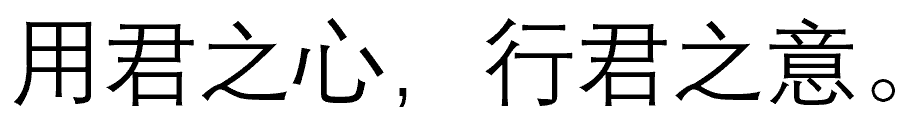
\includegraphics{preface_e1_1}
\end{figure}
\newpage
\tableofcontents
\newpage \section{Week1}
\subsection{Lecture 1}
\subsubsection{Course materials}
\paragraph{Bi-conditional}
$$ P \Leftrightarrow Q =(P \to Q) \land (Q\to P)$$
Which reads P if and only if Q.
\subsubsection{Exercises}
\paragraph{0.2.1}
For each sentence below, decide whether it is an atomic statement, a
molecular statement, or not a statement at all.\newline
(a) Customers must wear shoes.\newline
(b) The customers wore shoes.\newline
(c) The customers wore shoes and they wore socks.\newline
Solution:\newline
(a) This is not a statement. It is an imperative sentence, but is not either
true or false. It doesn’t matter that this might actually be the rule or
not. Note that “The rule is that all customers must wear shoes” is a
statement.\newline
(b) This is a statement, as it is either true or false. It is an atomic statement
because it cannot be divided into smaller statements.\newline
(c) This is again a statement, but this time it is molecular. In fact, it is a
conjunction, as we can write it as “The customers wore shoes and
the customers wore socks.”
\paragraph{0.2.3}
Suppose P and Q are the statements: P: Jack passed math. Q: Jill passed math.\newline
(a) Translate “Jack and Jill both passed math” into symbols.\newline
(b) Translate “If Jack passed math, then Jill did not” into symbols.\newline
(c) Translate “$P \lor Q$” into English.\newline
(d) Translate “$\lnot (P \land Q) \to Q$” into English.\newline
Solution:\newline
(a) $P \land Q$.\newline
(b) $P\to \lnot Q$\newline
(c) Jack passed math or Jill passed math (or both).\newline
(d) If Jack and Jill did not both pass math, then Jill did.\newline
(e) i. Nothing else.\newline
ii. Jack did not pass math either
\paragraph{0.2.4}
Determine whether each molecular statement below is true or false, or
whether it is impossible to determine. Assume you do not know what
my favorite number is (but you do know that 13 is prime).\newline
(a) If 13 is prime, then 13 is my favorite number.\newline
(b) If 13 is my favorite number, then 13 is prime.\newline
(c) If 13 is not prime, then 13 is my favorite number.\newline
(d) 13 is my favorite number or 13 is prime.\newline
(e) 13 is my favorite number and 13 is prime.\newline
(f) 7 is my favorite number and 13 is not prime.\newline
(g) 13 is my favorite number or 13 is not my favorite number\newline
Solution:\newline
(a) It is impossible to tell. The hypothesis of the implication is true.
Thus the implication will be true if the conclusion is true (if 13 is my
favorite number) and false otherwise.\newline
(b) This is true, no matter whether 13 is my favorite number or not. Any
implication with a true conclusion is true.\newline
(c) This is true, again, no matter whether 13 is my favorite number or
not. Any implication with a false hypothesis is true.\newline
(d) For a disjunction to be true, we just need one or the other (or both)
of the parts to be true. Thus this is a true statement.\newline
(e) We cannot tell. The statement would be true if 13 is my favorite
number, and false if not (since a conjunction needs both parts to be
true to be true).
\paragraph{0.2.5}
In my safe is a sheet of paper with two shapes drawn on it in colored
crayon. One is a square, and the other is a triangle. Each shape is
drawn in a single color. Suppose you believe me when I tell you that if
the square is blue, then the triangle is green. What do you therefore know
about the truth value of the following statements?\newline
(a) The square and the triangle are both blue.\newline
(b) The square and the triangle are both green.\newline
(c) If the triangle is not green, then the square is not blue.\newline
(d) If the triangle is green, then the square is blue.\newline
(e) The square is not blue or the triangle is green.\newline
Solution:\newline
The main thing to realize is that we don’t know the colors of these
two shapes, but we do know that we are in one of three cases: We could
have a blue square and green triangle. We could have a square that was
not blue but a green triangle. Or we could have a square that was not blue
and a triangle that was not green. The case in which the square is blue but
the triangle is not green cannot occur, as that would make the statement
false.\newline
(a) This must be false. In fact, this is the negation of the original
implication.\newline
(b) This might be true or might be false.\newline
(c) True. This is the contrapositive of the original statement, which is
logically equivalent to it.\newline
(d) We do not know. This is the converse of the original statement. In
particular, if the square is not blue but the triangle is green, then the
original statement is true but the converse is false.\newline
(e) True. This is logically equivalent to the original statement.
\paragraph{0.2.6}
Again, suppose the statement “if the square is blue, then the triangle
is green” is true. This time however, assume the converse is false.
Classify each statement below as true or false (if possible).\newline
(a) The square is blue if and only if the triangle is green.\newline
(b) The square is blue if and only if the triangle is not green.\newline
(c) The square is blue.\newline
(d) The triangle is green.\newline
Solution:\newline
The only way for an implication $P \to Q$ to be true but its converse
to be false is for Q to be true and P to be false. Thus:\newline
(a) False.\newline
(b) True.\newline
(c) False.\newline
(d) True.
\paragraph{0.2.7}
Consider the statement, “If you will give me a cow, then I will give you
magic beans.” Decide whether each statement below is the converse,
the contrapositive, or neither.\newline
(a) If you will give me a cow, then I will not give you magic beans.\newline
(b) If I will not give you magic beans, then you will not give me a
cow.\newline
(c) If I will give you magic beans, then you will give me a cow.\newline
(d) If you will not give me a cow, then I will not give you magic
beans.\newline
(e) You will give me a cow and I will not give you magic beans.\newline
(f) If I will give you magic beans, then you will not give me a cow.\newline
Solution:\newline
The converse is “If I will give you magic beans, then you will
give me a cow.” The contrapositive is “If I will not give you magic beans,
then you will not give me a cow.” All the other statements are neither the
converse nor contrapositive.
\paragraph{0.2.9}
You have discovered an old paper on graph theory that discusses the
viscosity of a graph (which for all you know, is something completely
made up by the author). A theorem in the paper claims that “if a
graph satisfies condition (V), then the graph is viscous.” Which of
the following are equivalent ways of stating this claim? Which are
equivalent to the converse of the claim?\newline
(a) A graph is viscous only if it satisfies condition (V).\newline
(b) A graph is viscous if it satisfies condition (V).\newline
(c) For a graph to be viscous, it is necessary that it satisfies condition
(V).\newline
(d) For a graph to be viscous, it is sufficient for it to satisfy condition
(V).\newline
(e) Satisfying condition (V) is a sufficient condition for a graph to
be viscous.\newline
(f) Satisfying condition (V) is a necessary condition for a graph to
be viscous.\newline
(g) Every viscous graph satisfies condition (V).\newline
(h) Only viscous graphs satisfy condition (V).\newline
Solution:\newline
(a) Equivalent to the converse.\newline
(b) Equivalent to the original theorem.\newline
(c) Equivalent to the converse.\newline
(d) Equivalent to the original theorem.\newline
(e) Equivalent to the original theorem.\newline
(f) Equivalent to the converse.\newline
(g) Equivalent to the converse.\newline
(h) Equivalent to the original theorem.
\paragraph{0.2.10}
Write each of the following statements in the form, “if . . . , then . . . .”
Careful, some of the statements might be false (which is alright for the
purposes of this question).\newline
(a) To lose weight, you must exercise.\newline
(b) To lose weight, all you need to do is exercise.\newline
(c) Every American is patriotic.\newline
(d) You are patriotic only if you are American.\newline
(e) The set of rational numbers is a subset of the real numbers.\newline
(f) A number is prime if it is not even.\newline
(g) Either the Broncos will win the Super Bowl, or they won’t play
in the Super Bowl.\newline
Solution:\newline
(a) If you have lost weight, then you exercised.\newline
(b) If you exercise, then you will lose weight.\newline
(c) If you are American, then you are patriotic.\newline
(d) If you are patriotic, then you are American.\newline
(e) If a number is rational, then it is real.\newline
(f) If a number is not even, then it is prime. (Or the contrapositive: if a
number is not prime, then it is even.)\newline
(g) If the Broncos don’t win the Super Bowl, then they didn’t play in the
Super Bowl. Alternatively, if the Broncos play in the Super Bowl,
then they will win the Super Bowl.
\subsection{Lecture 2}
\subsubsection{Course materials}
\paragraph{Necessity and Sufficiency}
“P is necessary for Q” means $Q \to P$.\newline
“P is sufficient for Q” means $P \to Q$.\newline
"If P is necessary and sufficient for Q, then $P \Leftrightarrow Q$."
\subsubsection{Exercises}
\paragraph{0.2.14}
For a given predicate P(x), you might believe that the statements $\forall xP(x)$ or $\exists xP(x)$ are either true or false. How would you decide if
you were correct in each case? You have four choices: you could give an example of an element n in the domain for which P(n) is true or for which P(n) if false, or you could argue that no matter what n is, P(n) is true or is false.\newline
(a) What would you need to do to prove $\forall x P(x)$ is true?\newline
(b) What would you need to do to prove $\forall x P(x)$ is false?\newline
(c) What would you need to do to prove $\exists x P(x)$ is true?\newline
(d) What would you need to do to prove $\exists x P(x)$ is false?\newline
\paragraph{0.2.16}
Translate into symbols. Use E(x) for “x is even” and O(x) for “x is
odd.”\newline
(a) No number is both even and odd.\newline
(b) One more than any even number is an odd number.\newline
(c) There is prime number that is even.\newline
(d) Between any two numbers there is a third number.\newline
(e) There is no number between a number and one more than that
number.\newline
Solution:\newline
(a)$\lnot\exists x(E(x)\land O(x)$\newline
(b)$\forall x(E(x)\to O(x+1))$\newline
(c)$\exists x(E(x)\land P(x))$ (where P(x) means “x is prime”)\newline
(d)$\forall x \forall y \exists z (x < z < y \land y < z < x)$\newline
(e)$\forall x \exists y (x<y<x+1)$
\paragraph{0.3.1}
Let A  \{1, 4, 9\} and B  \{1, 3, 6, 10\}. Find each of the following sets.
$ (a) A \cup B$\newline
$ (b) A \cap B$\newline
$ (c) A \backslash B$\newline
$(d) B \backslash A$\newline
Solution:\newline
$(a) \{1, 3, 4, 6, 9, 10\} $\newline
$(b) \{1\}$\newline
$(c) \{4, 9\}$\newline
$(d) \{3, 6, 10\}$\newline
\paragraph{0.3.2}
Find the least element of each of the following sets, if there is one.\newline
(a)$\{n\in N:n^2-3\ge 2\}$\newline
(b)$\{n\in N:n^2-5\in N\}$\newline
(c)$\{n^2+1\in N\}$\newline
(d)$\{n\in N:n=k^2+1 \ for\ some \ K\in N\}$\newline
Solution:\newline
(a) This is the set {3, 4, 5, . . .} since we need each element to be a natural number whose square is at least three more than 2. Since $3^2-3=6$ but $2^2-3=1$we see that the first such natural number is 3.\newline
(b)We get the same set as we did in the previous part, and the smallest
non-negative number for which $n^2-5$ is a natural numbers is 3.\newline
(c)This is the set {1, 2, 5, 10, . . .}, namely the set of numbers that are
the result of squaring and adding 1 to a natural number. Thus the least element of the set is 1.\newline
(d)Now we are looking for natural numbers that are equal to taking some natural number, squaring it and adding 1. That is,
{1, 2, 5, 10, . . .}, the same set as the previous part. So again, the least
element is 1
\paragraph{0.3.3}
Find the following cardinalities:\newline
(a) $\|A\|$ when $A=\{4, 5, 6, . . . , 37\}$.\newline
(b) $\|A\|$ when $A=\{x\in Z : -2 \leq x \leq 100\}$.\newline
(c) $\|A \cap B\|$ when $A=\{x\in N : x \leq 20\}$ and B  $\{x\in N : x is prime\}$.\newline
Solution:\newline
(a) 34. Note that $37-4=33$, but this calculation would not include 4
itself.\newline
(b) 103. Again, you could compute this by $100 - (-2) + 1$, or simply
count: 100 numbers from 1 through 100, plus -2, -1, and 0.\newline
(c) 8. There are 8 primes not greater than 20: $\{2, 3, 5, 7, 11, 13, 17, 19\}$.
\subsection{Lecture 3}
\subsubsection{Course materials}
\paragraph{Knights and Knaves}
Two trolls, A and B, stand before you.\newline
Troll A: If we are cousins, then we are both knaves.\newline
Troll B: We are cousins or we are both knaves.
\newline
Can you finish C, SA and SB so that the table shows exactly one of the two trolls is a knight.\newline
A:A is a knight\newline
B:B is a knight.\newline
C:A and B are both cousins.\newline
SA:$xor(\lnot A,C \to \lnot A \land \lnot B)$\newline
SB:$xor(\lnot B,C\lor \lnot A \land \lnot B)$\newline
Solution:\newline
A|B|C|SA|SB|\newline
T|T|T|F |F |\newline
T|T|F|T |F |\newline
T|F|T|F |F |\newline
T|F|F|T |T |\newline
F|T|T|T |T |\newline
F|T|F|F |F |\newline
F|F|T|F |F |\newline
F|F|F|F |F |
\paragraph{De Morgan’s Laws}:\newline
1:$\lnot (P\land Q)=\lnot P \lor \lnot Q$ \newline
2:$\lnot (P\lor Q)=\lnot P \land \lnot Q$\newline
Prove that the statements $\lnot (P \to Q)$ and $P \land \lnot Q$ are logically equivalent\newline
Prove:\newline
$\lnot (P \to Q)$=$\lnot (\lnot P \lor Q)$\newline
$\Longrightarrow \lnot \lnot P \land \lnot Q$\newline
$\Longrightarrow P \land \lnot Q$\newline
Q.E.D.
\subsubsection{Exercises}
\paragraph{3.1.1}
Consider the statement about a party, “If it’s your birthday or there
will be cake, then there will be cake.”\newline
(a) Translate the above statement into symbols. Clearly state which
statement is P and which is Q.\newline
(b) Make a truth table for the statement.\newline
(c) Assuming the statement is true, what (if anything) can you
conclude if there will be cake?\newline
(d) Assuming the statement is true, what (if anything) can you
conclude if there will not be cake?\newline
(e) Suppose you found out that the statement was a lie. What can
you conclude?\newline
Solution:\newline
(a) P: it’s your birthday; Q: there will be cake. $(P \lor Q) \to Q$\newline
(b)\newline
P|Q|$(P \land Q) \to Q$\newline
T|T|T\newline
T|F|F\newline
F|T|T\newline
F|F|T\newline
(c) Only that there will be cake.\newline
(d) It’s NOT your birthday!\newline
(e) It’s your birthday, but the cake is a lie.
\paragraph{3.1.2}
Make a truth table for the statement $(P \lor Q) \to (P \land Q)$.\newline
Solution:\newline
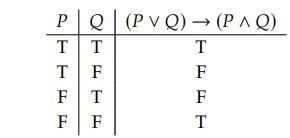
\includegraphics{3.1.2}
\paragraph{3.1.3}
Make a truth table for the statement $\lnot P \land (Q \to P)$. What can you
conclude about P and Q if you know the statement is true?\newline
Solution:\newline
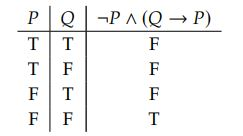
\includegraphics{3.1.3}\newline
If the statement is true, then both P and Q are false.
\paragraph{3.1.8}
Simplify the following statements (so that negation only appears right
before variables).\newline
(a) $\lnot(P \to \lnot Q)$.\newline
(b) $(\lnot P \lor \lnot Q) \to \lnot (\lnot Q \land R)$.\newline
(c) $\lnot((P \to \lnot Q) \lor \lnot(R \land \lnot R))$.\newline
(d) It is false that if Sam is not a man then Chris is a woman, and
that Chris is not a woman.\newline
Solution:\newline
(a) $P \land Q$.\newline
(b) $(\lnot P\lor \lnot R) \to (Q \lor \lnot R)$ or, replacing the implication with a disjunction
first: $(P \land Q) \lor (Q \lor \lnot R)$.\newline
(c) $(P \land Q) \land (R \land \lnot R)$. This is necessarily false, so it is also equivalent
to $P \land \lnot P$.\newline
(d) Either Sam is a woman and Chris is a man, or Chris is a woman.
\paragraph{3.1.12}
Determine if the following deduction rule is valid:
$$P \lor Q$$
$$\lnot P$$
$$\_\_\_\_\_$$
$$\ therefore\ Q$$
Solution:\newline
the deduction rule is valid. To see this, make a truth table which
contains $P \lor Q$ and $\lnot P$ (and P and Q of course). Look at the truth value of
Q in each of the rows that have $P \lor Q$ and $\lnot P$ true.
\subsection{Lecture 4}
\subsubsection{Course materials}
\paragraph{Example 3.1.8}:\newline
$\lnot \exists x \forall y P(x,y)$\newline
$\Longrightarrow \forall x \exists y \lnot P(x,y)$\newline
Idea: $\lnot \exists x \forall y P(x,y) \leftrightarrow \forall x (\lnot(\forall y P(x,y) \leftrightarrow \forall x \exists y \lnot P(x,y)$ 
\paragraph{Example 3.2.2 n is even}
For all integers n, if n is even, then $n^2$ is even.\newline
Proof:\newline
Since n is even, then $\exists i \in Z$, n=2i.\newline
Thus,$n^2=(2i)^2=4i^2=2*(2i^2)$.\newline
Therefore, $n^2$ is even since $(2i^2)$ is an integer.\newline
Q.E.D.
\paragraph{Example 3.2.2 n is odd}
For all integers n, if n is odd, then $n^2$ is odd.\newline
Proof:\newline
Since n is odd, then $\exists i \in Z$, $n=2i+1$.\newline
Thus,$n^2=(2i+1)^2=4i^2+4i+1=2*(2i^2+2i)+1$.\newline
Therefore, $n^2$ is odd since $2(2i^2+2i)+1$ is an odd integer.\newline
Q.E.D.
\paragraph{Example 3.2.4 \& 3.2.5 Prove by contrapositive}:\newline
If $n^2$ is even, then n is even. $\leftrightarrow$ If n is odd, then $n^2$ is odd.\newline
For all integer a and b, if a+b is odd, then a is odd or b is odd.\newline
Idea:\newline
Let P be a+b is odd, Q be a is odd or b is odd. \newline
P $\to$ Q $\Leftrightarrow$ $\lnot Q \to \lnot P$\newline
$\Rightarrow \lnot Q \leftrightarrow \lnot(O(a)\lor O(b))\leftrightarrow E(a)\land E(b)$ \newline
$\lnot P: \lnot O(a+b) \leftrightarrow E(a+b)$\newline
$\lnot Q \to \lnot P \Leftrightarrow E(a)\land E(b) \to E(a+b)$ which is obvious.
\paragraph{Example 3.2.7 \& 3.2.8 Prove by Contradiction}:\newline
Prove that $\sqrt{2}$ is irrational.\newline
Prove:\newline
Assume $\sqrt{2}$ is rational, \newline
thus let i and j be two integers, which means $\exists i,j \in Q$, $\sqrt{2}=\frac{i}{j}$ and that i and j that gcd(i,j)=1.\newline
Tus, $i=\sqrt{2}j^2\to i^2=2j^2$\newline
Thus, i must be even\newline
Thus, $Let \ i=2k$ for some k $\in Z$\newline
Thus $(2k^2)=2j^2 \leftrightarrow j^2=2K^2$ which means j is even.\newline
This is contradiction to gcd(i,j)=1.\newline
Therefore, $\sqrt{2}$ is irrational.\newline
Prove that there are no integers x and y such that $x^2=4y+2$\newline
Prove:\newline
Assume $\exists x,y \in Z$, such that $x^2=4y+2=2(2y+1)$\newline
Thus, x must be a even number.\newline
Thus,$\exists i \in Z$ such that, $x=2i$\newline
Thus, $(2i)^2=2(2y+1) \leftrightarrow 4i^2=2(2y+1) \leftrightarrow 2i^2=2y+1$\newline
which is a contradiction to the assumption.
\paragraph{The Pigeonhole Principle}:\newline
If more than n pigeon fly into n pigeon
holes, then at least one pigeon hole will contain at least two pigeon.
\subsubsection{Exercises}
\paragraph{3.2.1}
Consider the statement “for all integers a and b, if a + b is even, then a
and b are even”\newline
(a) Write the contrapositive of the statement.\newline
(b) Write the converse of the statement.\newline
(c) Write the negation of the statement.\newline
(d) Is the original statement true or false? Prove your answer.\newline
(e) Is the contrapositive of the original statement true or false? Prove
your answer.\newline
(f) Is the converse of the original statement true or false? Prove
your answer.\newline
(g) Is the negation of the original statement true or false? Prove
your answer\newline
Solution:\newline
(a) For all integers a and b, if a or b is not even, then a + b is not even.\newline
(b) For all integers a and b, if a and b are even, then a + b is even.\newline
(c) There are numbers a and b such that a + b is even but a and b are
not both even.\newline
(d) False. For example, a = 3 and b = 5. a + b = 8, but neither a nor b
are even.\newline
(e) False, since it is equivalent to the original statement.\newline
(f) True. Let a and b be integers. Assume both are even. Then a  2k\newline
and b = 2j for some integers k and j. But then a+b = 2k+2j = 2(k+j)
which is even.\newline
(g) True, since the statement is false.
\paragraph{3.2.2}
For each of the statements below, say what method of proof you should
use to prove them. Then say how the proof starts and how it ends.
Bonus points for filling in the middle.
(a) There are no integers x and y such that x is a prime greater than
5 and x = 6y + 3.
(b) For all integers n, if n is a multiple of 3, then n can be written as
the sum of consecutive integers.
(c) For all integers a and b, if $a^2+b^2$
is odd, then a or b is odd.\newline
Solution:\newline
(a) Proof by contradiction. Start of proof: Assume, for the sake of
contradiction, that there are integers x and y such that x is a prime
greater than 5 and x = 6y+3. End of proof: . . . this is a contradiction,
so there are no such integers.\newline
(b) Direct proof. Start of proof: Let n be an integer. Assume n is a
multiple of 3. End of proof: Therefore n can be written as the sum of
consecutive integers.\newline
(c) Proof by contrapositive. Start of proof: Let a and b be integers.
Assume that a and b are even. End of proof: Therefore $a^2+b^2$
is even.
\paragraph{3.2.3}
Consider the statement: for all integers n, if n is even then 8n is even.\newline
(a) Prove the statement. What sort of proof are you using?\newline
(b) Is the converse true? Prove or disprove.\newline
Solution:\newline
(a) Direct proof.
Proof. p:proof:ckO Let n be an integer. Assume n is even. Then
n = 2k for some integer k. Thus 8n = 16k = 2(8k). Therefore 8n is even.\newline 
(b) The converse is false. That is, there is an integer n such that 8n is
even but n is odd. For example, consider n = 3. Then 8n = 24 which
is even but n = 3 is odd.
\paragraph{3.2.4}
The game TENZI comes with 40 six-sided dice (each numbered 1 to 6).\newline
Suppose you roll all 40 dice.\newline
(a) Prove that there will be at least seven dice that land on the same
number.\newline
(b) How many dice would you have to roll before you were guaranteed that some four of them would all match or all be different?
Prove your answer.\newline
Solution:\newline
(a) This is an example of the pigeonhole principle. We can prove it by
contrapositive.\newline
Proof. p:proof:ozg Suppose that each number only came up 6 or
fewer times. So there are at most six 1’s, six 2’s, and so on. That’s a
total of 36 dice, so you must not have rolled all 40 dice. QED\newline
(b) We can have 9 dice without any four matching or any four being all
different: three 1’s, three 2’s, three 3’s. We will prove that whenever
you roll 10 dice, you will always get four matching or all being
different.\newline
Proof. p:proof:UGp Suppose you roll 10 dice, but that there are NOT
four matching rolls. This means at most, there are three of any given
value. If we only had three different values, that would be only 9
dice, so there must be 4 different values, giving 4 dice that are all
different. QED
\paragraph{3.2.7}
Consider the statement: for all integers a and b, if a is even and b is a
multiple of 3, then ab is a multiple of 6.\newline
(a) Prove the statement. What sort of proof are you using?\newline
(b) State the converse. Is it true? Prove or disprove\newline
Idea:\newline
Part (a) should be a relatively easy direct proof. \newline
Look for a counterexample for part (b).
\paragraph{3.2.9}
Prove the statement: For all integers a, b, and c, if $a^2+b^2=c^2$ , then a or b is even\newline
Idea:\newline
A proof by contradiction would be reasonable here, because then
you get to assume that both a and b are odd. Deduce that $c^2$ is even, and therefore a multiple of 4 (why? and why is that a contradiction?).
\paragraph{3.2.13}
Prove that log(7) is irrational.\newline
Idea:\newline
Note that if $log(7)=\frac{a}{b}$
, then $7=10^\frac{a}{b}$. Can any power of 7 be the same as a power of 10?
\newpage \section{Week2}
\subsection{Lecture 5}
\subsubsection{Course materials}
\paragraph{Proposition 2.10}
$\binom{m}{n}=\binom{m}{m-n}$\newline
Combinatorial proof:\newline
LHS: Ways to invite n students out of m students to your party.\newline
RHS: Ways to choose m-n students out of m not to attend your party.
\paragraph{Proposition 2.10 Another Identity}
$n\binom{m}{n}=m\binom{m-1}{n-1}$\newline
Combinatorial proof:\newline
LHS: Ways to choose n students out of m students, then choose one of n students as their leader.\newline
RHS: From m students, we choose 1 as their leader. Then in the rest of m-1 students, we choose the rest n-1 people.
\paragraph{Think-pair-share}
Show that for $0<n<m$, $\binom{m}{n}=\binom{m-1}{n-1}+\binom{m-1}{n}$\newline
Combinatorial proof:\newline
LHS: ways to choose n of m students to form a committee.\newline
RHS: $\binom{m-1}{n-1}$ means assume I was chosen, then choose n-1 students from the rest m-1 students.$\binom{m-1}{n}$ means assume I was not chosen, then chose n people from the rest m-1 people.
\paragraph{Fibonacci number Think-pair-share}
Can you find a combinatorial proof that $F_{2n}=F_n^2+F^2_{n-1} (n\ge 2)$\newline
Combinatorial proof:\newline
LHS: it is the number of ways to tile a 1*2n grid.\newline
RHS: there are two cases, let's denote the middle point of the grid as A.\newline
1. If the middle exists a domino, then there are both n-1 places to be filled at both sides of A, the total ways is$$F_{n-1}\times F_{n-1}=F^2_{n-1}$$
2. If the middle doesn't have a domino, then there are both n places to be filled at both sides of A, the total ways is$$F_{n}\times F_{n}=F^2_{n}$$
Adding the two cases up we have the number of ways in total,  LHS =RHS.
\subsubsection{Exercises}
\paragraph{2.9.1}
The Hawaiian alphabet consists of 12 letters. How many six-character strings can
be made using the Hawaiian alphabet?\newline
Solution:\newline
$12^6$\newline
Label each letter in the Hawaiian alphabet as 1, 2, . . . , 12. Then, each string corresponds
to an element in
$$\underbrace{12\times \cdots \times 12}_{6}$$
\paragraph{2.9.3}
Matt is designing a website authentication system. He knows passwords are most
secure if they contain letters, numbers, and symbols. However, he doesn’t quite understand that this additional security is defeated if he specifies in which positions each
character type appears. He decides that valid passwords for his system will begin with
three letters (uppercase and lowercase both allowed), followed by two digits, followed
by one of 10 symbols, followed by two uppercase letters, followed by a digit, followed
by one of 10 symbols. How many different passwords are there for his website system?
How does this compare to the total number of strings of length 10 made from the alphabet of all uppercase and lowercase English letters, decimal digits, and 10 symbols?\newline
Solution:\newline
$52^3\times 10^3 \times 26^3 \times 10^2$\newline
$72^{10}$
\paragraph{2.9.5}
Suppose we are making license plates of the form $l_1 l_2 l_3 - d_1 d_2 d_3$ where $l_1 l_2 l_3$ are capital letters in the English alphabet and $d_1 d_2 d_3$ are decimal digits. subject to the restriction that at least one digit is nonzero and at least one letter is K. How many license plates can we make? \newline
Solution:\newline
$(26^3-25^3)\cdot (10^3-1)$
\paragraph{2.9.7}
How many string of the form $l_1 l_2 d_1 d_2 d_3 l_3 l_4 d_4 l_5 l_6$ are there where\newline
• for $1 \leq i \leq 6$, $l_i$
is an uppercase letter in the English alphabet;\newline
• for $1 \leq i \leq 4$, $d_i$
is a decimal digit;\newline
• $l_2$ is not a vowel (i.e., $l_2$ not in {A,E,I,O,U}); and the digits $d_1$, $d_2$, and $d_3$ are distinct (i.e., $d1 \neq d2 \neq d3$).\newline
Solution:\newline
$26^5\cdot 21 \cdot 10^2 \cdot 9 \cdot 8$
\paragraph{2.9.9}
A database uses 20-character strings as record identifiers. The valid characters in
these strings are upper-case letters in the English alphabet and decimal digits. (Recall
there are 26 letters in the English alphabet and 10 decimal digits.) How many valid
record identifiers are possible if a valid record identifier must meet all of the following
criteria:\newline
• Letter(s) from the set {A, E, I, O, U} occur in exactly three positions of the string.\newline
• The last three characters in the string are distinct decimal digits that do not appear elsewhere in the string.\newline
• The remaining characters of the string may be filled with any of the remaining
letters or decimal digits.\newline
Solution:\newline
$$\binom{17}{3}\cdot 5^3 \cdot 10 \cdot 9 \cdot 8 \cdot (7+21)^{14}$$
\paragraph{2.9.11}
A donut shop sells 12 types of donuts. A manager wants to buy six donuts, one
each for himself and his five employees.\newline
(a) Suppose that he does this by selecting a specific type of donut for each person.
(He can select the same type of donut for more than one person.) In how many
ways can he do this?\newline
(b) How many ways could he select the donuts if he wants to ensure that he chooses
a different type of donut for each person?\newline
(c) Suppose instead that he wishes to select one donut of each of six different types
and place them in the breakroom. In how many ways can he do this? (The order
of the donuts in the box is irrelevant.)\newline
Solution:\newline
(a)$12^6$\newline
(b)$P(12,6)$\newline
(c)$\binom{12}{6}$
\paragraph{2.9.13}
Twenty students compete in a programming competition in which the top four
students are recognized with trophies for first, second, third, and fourth places.\newline
(a) How many different outcomes are there for the top four places?\newline
(b) At the last minute, the judges decide that they will award honorable mention
certificates to four individuals who did not receive trophies. In how many ways
can the honorable mention recipients be selected (after the top four places have
been determined)? How many total outcomes (trophies plus certificates) are there
then?\newline
Solution:\newline
(a) $P(20,4)$\newline
(b) $\binom{16}{4}$ Total: $P(20,4)\cdot \binom{16}{4}$
\subsection{Lecture 6}
\subsubsection{Course materials}
\paragraph{Example 2.1.7 and 2.1.9}
Prove that $\underbrace{\binom{n}{0}+\cdots+\binom{n}{n}}_{n}=2^n$\newline
Combinatorial proof:\newline
RHS: $2^n$ is the amount of binary string of length n.\newline
LHS: $\binom{n}{k},k\in N^*, k\leq n$ means the ways we set k binary string set (e.g. k=1, others =0) with the length n, k begins with zero, then ends with n. \newline
Then we add them up, which is equal to the amount of the binary string of length n.\newline
$\therefore$ RHS = LHS.\newline
Prove that $$\overbrace{\binom{n}{0}\cdot 2^0 +\cdots +\binom{n}{n}\cdot 2^n}^{n}=3^n$$\newline
Combinatorial proof:\newline
RHS: $3^n$ is the amount of ternary string (e.g.\{"0","1","2"\}) of length n.\newline
LHS: $\binom{n}{k}\cdot 2^k$ is the amount of ternary string containing "0", "0" ($\binom{n}{k}$ means k positions out of n positions) ($2^k$ means the amount of the binary string). While n-k means it does not contain "0","0". We add them up,then we can get the amount of the ternary string.\newline
Therefore, LHS=RHS.\newline
ChatGPT proof:\newline
One way to prove $\binom{n}{0}\cdot 2^0 +\cdots +\binom{n}{n}\cdot 2^n = 3^n$ is to use the combinatorial argument that the left-hand side counts the number of ways to color the elements of a set with two colors, red and blue, and the right-hand side counts the number of ways to color the elements of a set with three colors, red, blue, and green.\newline
To see this, consider an $n$-element set $S = \{s_1, s_2, \dots, s_n\}$. Each way of coloring the elements of $S$ with two colors, red and blue, can be uniquely identified by a binary vector of length $n$ with a $1$ in the $i$-th position if $s_i$ is colored red and a $0$ if $s_i$ is colored blue.\newline
Therefore, there are $2^n$ ways to color the elements of $S$ with two colors, red and blue.\newline
Now, we can color the elements of $S$ with three colors, red, blue and green, each one of the red or blue element can be colored with green, thus for each element in the set we have three options, so the number of ways to color the elements of $S$ with three colors is $3^n$.\newline
Therefore, the number of ways to color the elements of $S$ with two colors, red and blue is equal to the number of ways to color the elements of $S$ with three colors, red, blue, and green, which is $\binom{n}{0}\cdot 2^0 +\cdots +\binom{n}{n}\cdot 2^n =3^n$.
\paragraph{Exanple 2.1.8}
Prove that $\binom{n}{k+1}=\underbrace{\binom{k}{k}+\binom{k+1}{k}+\cdots + \binom{n-1}{k}}_{n-k}$\newline
Combinatorial proof:\newline
ChatGPT proof:\newline
To prove that $\binom{n}{k+1} = \binom{k}{k} + \binom{k+1}{k} + \cdots + \binom{n-1}{k}$, we can use the combinatorial definition of binomial coefficients.\newline
The binomial coefficient $\binom{n}{k}$ counts the number of ways to choose a subset of $k$ elements from a set of $n$ elements.\newline
One way to choose a subset of $k+1$ elements from a set of $n$ elements is to first choose one of the $n$ elements, and then choose a subset of $k$ elements from the remaining $n-1$ elements.\newline
Therefore, the number of ways to choose a subset of $k+1$ elements from a set of $n$ elements is equal to the sum of the number of ways to choose a subset of $k$ elements from a set of $k$ elements, plus the number of ways to choose a subset of $k$ elements from a set of $k+1$ elements, plus the number of ways to choose a subset of $k$ elements from a set of $k+2$ elements, and so on, until the number of ways to choose a subset of $k$ elements from a set of $n-1$ elements.\newline
This can be written mathematically as:
$$\binom{n}{k+1} = \binom{k}{k} + \binom{k+1}{k} + \cdots + \binom{n-1}{k}$$
Where the binomial coefficient $\binom{k}{k}$ counts the number of ways to choose a subset of $k$ elements from a set of $k$ elements, and so on.\newline
Therefore, we have proven that $\binom{n}{k+1} = \binom{k}{k} + \binom{k+1}{k} + \cdots + \binom{n-1}{k}$
\paragraph{Example 2.2.0}
give a Combinatorial proof of $\binom{2n}{n} =\binom{n}{0}^2+\binom{n}{1}^2+\cdots +\binom{n}{n}^2$\newline
ChatGPT proof:\newline
We can use the combinatorial proof method of counting to prove the identity $\binom{2n}{n} =\binom{n}{0}^2+\binom{n}{1}^2+\cdots +\binom{n}{n}^2$.\newline
Consider a set of $2n$ elements. We want to count the number of ways to choose a subset of $n$ elements. We can do this by counting the number of subsets with a certain number of elements, and then summing the counts.\newline
Let's fix the number of elements in the subset to be $k$, where $0 \leq k \leq n$. The number of subsets with $k$ elements is $\binom{n}{k}^2$. This is because for each of the $k$ elements, we have two options: it can be in the subset or not. So there are $2^k$ ways to choose the subset with $k$ elements. Since there are $n$ elements from which to choose, the number of subsets with $k$ elements is $\binom{n}{k}^2$.
\newline
Therefore, the total number of subsets of $n$ elements is $\binom{n}{0}^2+\binom{n}{1}^2+\cdots +\binom{n}{n}^2$. But this is also equal to $\binom{2n}{n}$, which completes the proof.
\paragraph{Bars and balls argument – The formula 1}
Given m identical coin and n distinct people, the number of ways to distribute the coin such that no people is empty-handed. \newline
The formula will be $$\binom{m-1}{n-1}$$
For m coins, we can insert n-1 bars into m-1 gaps.
\paragraph{Integer composition 1}
How many integer solutions are there for
$$x_1+x_2+\cdots+x_n=m, m\in Z$$
solution:
$$\binom{m-1}{n-1}$$
\paragraph{Bars and balls argument - The formula 2}
In how many ways can Amanda distribute her coins, if she is allowed to give no coin to her daughter.\newline
We can count the ways of inserting two blocks in 11 gaps and
allowing that the two blocks is at the same gap.\newline
Solution:\newline
$$\binom{m+n-1}{n-1}$$, which is equal to
$$\binom{m+1}{n-1}+\cdots +\binom{m+1}{1}$$
(This is known as the Hockey Stick Identity)\newline
This is equal to already give every body a coin and then calculate with formula1.
$$\binom{m+n-1}{n-1}$$
\paragraph{Integer composition 2}
How many integer solutions are there for$$x_1+x_2+\cdots+x_n=m, m\in Z$$
solution:\newline
$$\binom{m+n-1}{n-1}$$
\subsubsection{Exercises}
\paragraph{2.9.15}
Suppose that a teacher wishes to distribute 25 identical pencils to Ahmed, Barbara,
Casper, and Dieter such that Ahmed and Dieter receive at least one pencil each, Casper
receives no more than five pencils, and Barbara receives at least four pencils. In how
many ways can such a distribution be made?\newline
Solution:\newline
$$\binom{25+1-3-1}{4-1}-\binom{25-5-3-1}{4-1}$$ which is equal to
$$\binom{22}{3}-\binom{16}{3}$$
\paragraph{2.9.17}
How many integer solutions are there to the equation
$$x_1+x_2+x_3+x_4=132$$
provided that $x1>0, x2,x3,x4\ge 0$ and what if we add the restriction $x4<17$\newline
Solution:\newline
$$\binom{132+3-1}{4-1}=\binom{134}{3}$$
$$\binom{132+3-1}{4-1}-\binom{132+2-16-1}{4-1}=\binom{134}{3}-\binom{117}{3}$$
\paragraph{2.9.19}
A teacher has 450 identical pieces of candy. He wants to distribute them to his class
of 65 students, although he is willing to take some leftover candy home. (He does not
insist on taking any candy home, however.) The student who won a contest in the last
class is to receive at least 10 pieces of candy as a reward. Of the remaining students, 34
of them insist on receiving at least one piece of candy, while the remaining 30 students
are willing to receive no candy.\newline
(a) In how many ways can he distribute the candy?\newline
(b) In how many ways can he distribute the candy if, in addition to the conditions
above, one of his students is diabetic and can receive at most 7 pieces of candy?
(This student is one of the 34 who insist on receiving at least one piece of candy.)\newline
Solution:\newline
(a) $$\binom{450+30-9-1+1}{65-1}=\binom{471}{64}$$
(b)$$\binom{471}{64}-\binom{471-7}{64}=\binom{471}{64}-\binom{464}{64}$$
\paragraph{2.9.21}
Let m and w be positive integers. Give a combinatorial argument to prove that for
integers $k \ge 0$,
$$\sum_{j=0}^{k}{\binom{m}{j}\cdot \binom{w}{k-j}}=\binom{m+w}{k}$$
Solution:\newline
Both sides count the number of ways to choose k people from a group of m + w people. The
right-hand side counts it directly since it is the number of ways to choose a k-element subset
from a set of m + w elements. The left hand side counts it by dividing the m + w people into
two groups: m men and w women. It then counts the number of ways to choose j men and
k - j women (which is k people). Doing this for all j is mutually exclusive, so we may sum
up all these scenarios to count the total number of ways to choose k people from this group.
\subsection{Lecture 7}
\subsubsection{Course material}
\paragraph{Lattice paths}
For string with alphabet $\{U, R\}$ (Up, Right) to correspond to a lattice
path from $(0, 0)$ to $(m, n)$, it must satisfy\newline
its length must be $m+n$ \newline
it contains m R and n U.\newline
the number of lattice paths from (0, 0) to (m,n) is $$\binom{m+n}{m}=\binom{m+n}{n}$$
How many lattice paths from (0,0) to (5,4) are there that do
not pass through (2,3)?
$$\binom{9}{5}-\binom{5}{2}\binom{4}{3}$$
Explanation: $\binom{5}{2}=\binom{3+2}{2}=\binom{3+2}{3}$ and $\binom{4}{3}=\binom{5-2+4-3}{5-2}=\binom{5-2+4-3}{4-3}$
\paragraph{Catalan Numbers - Good paths}:\newline
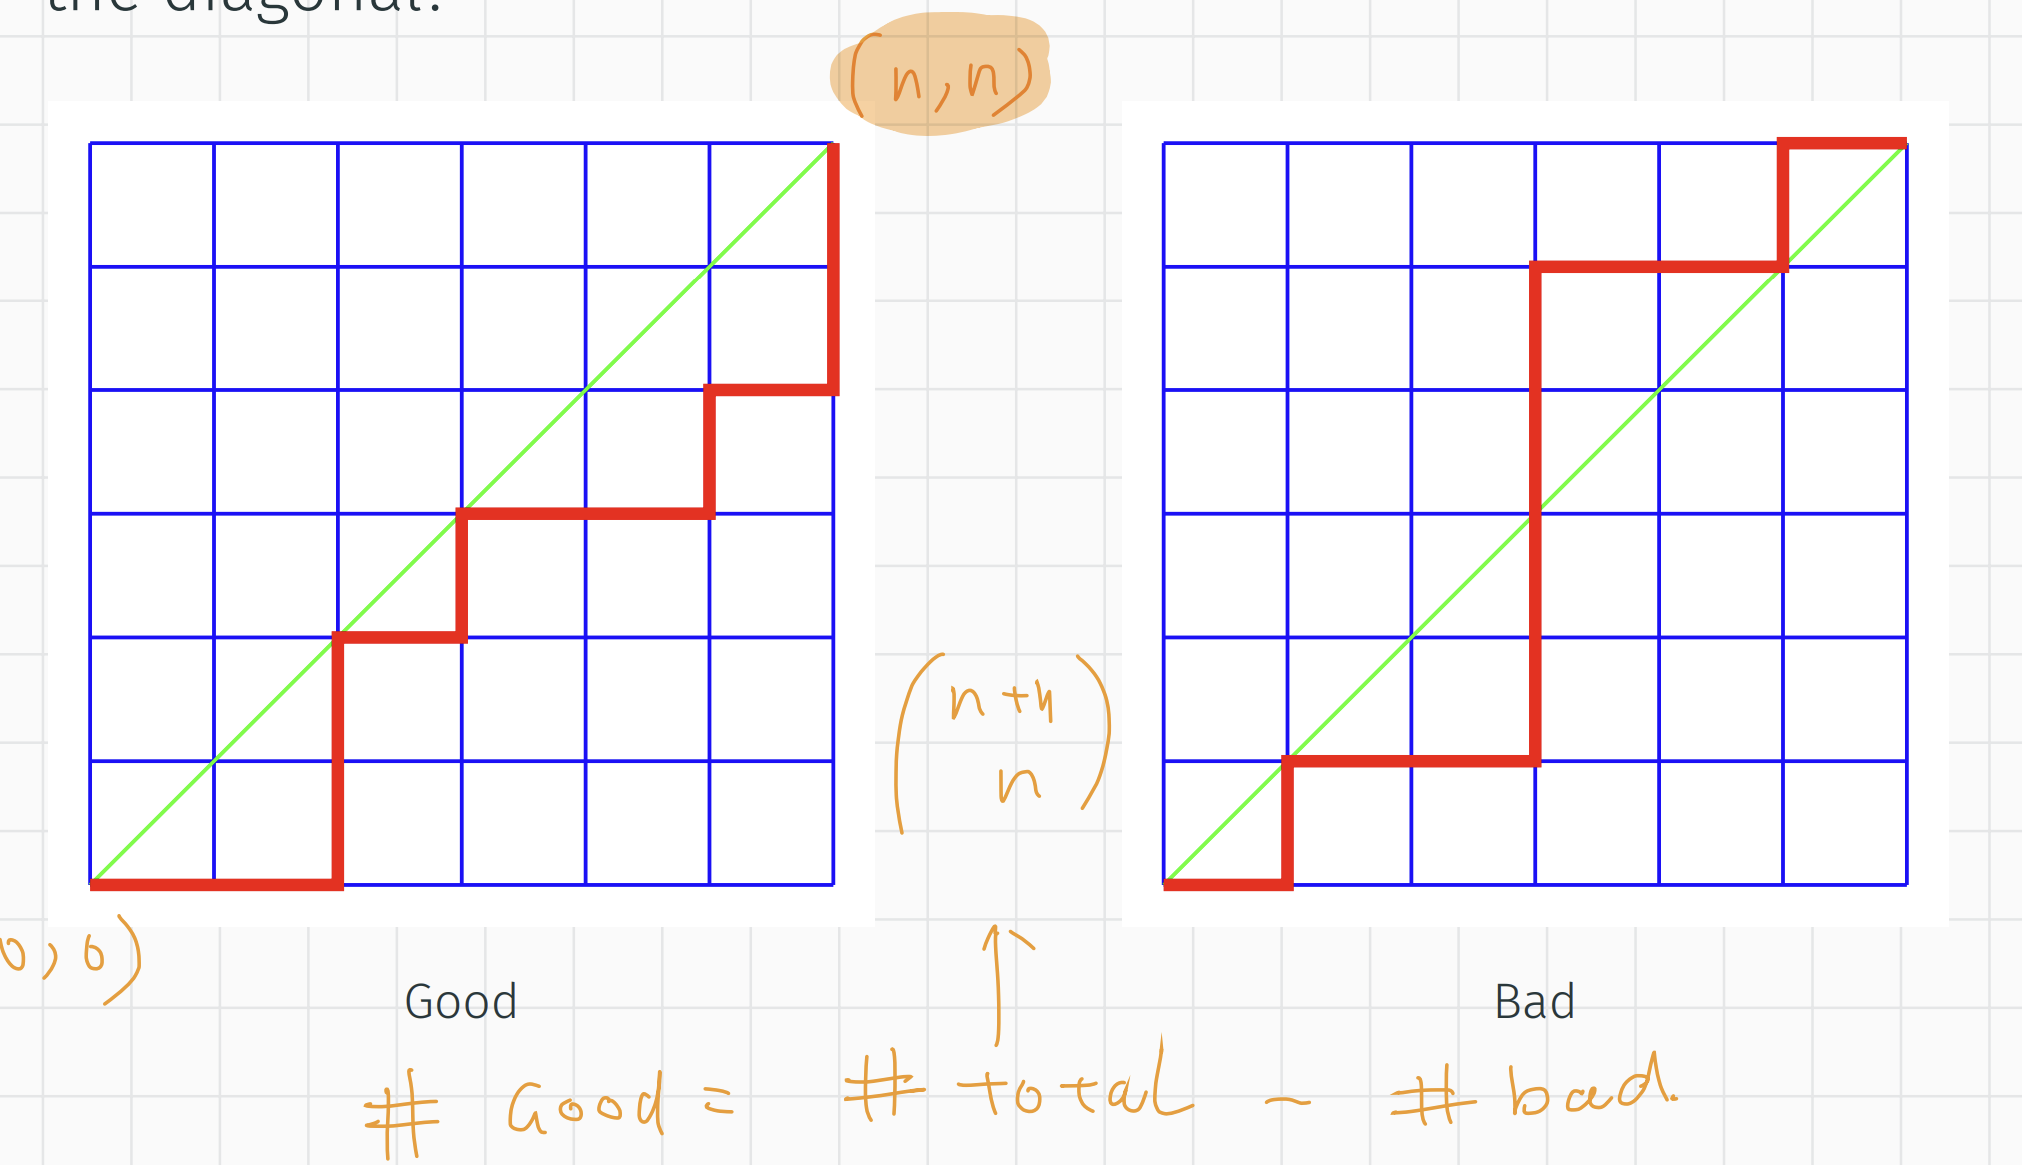
\includegraphics{0001}\newline
Crossing point:\newline
The bad path must first cross the diagonal and arrive at (j, j + 1)
for some j. This is the crossing point.\newline
the number good path is the Catalan Number
$$C(n)=Allpaths-Badpaths=\frac{\binom{2n}{n}}{n+1}$$
\paragraph{Catalan Numbers - Dyck path}:\newline
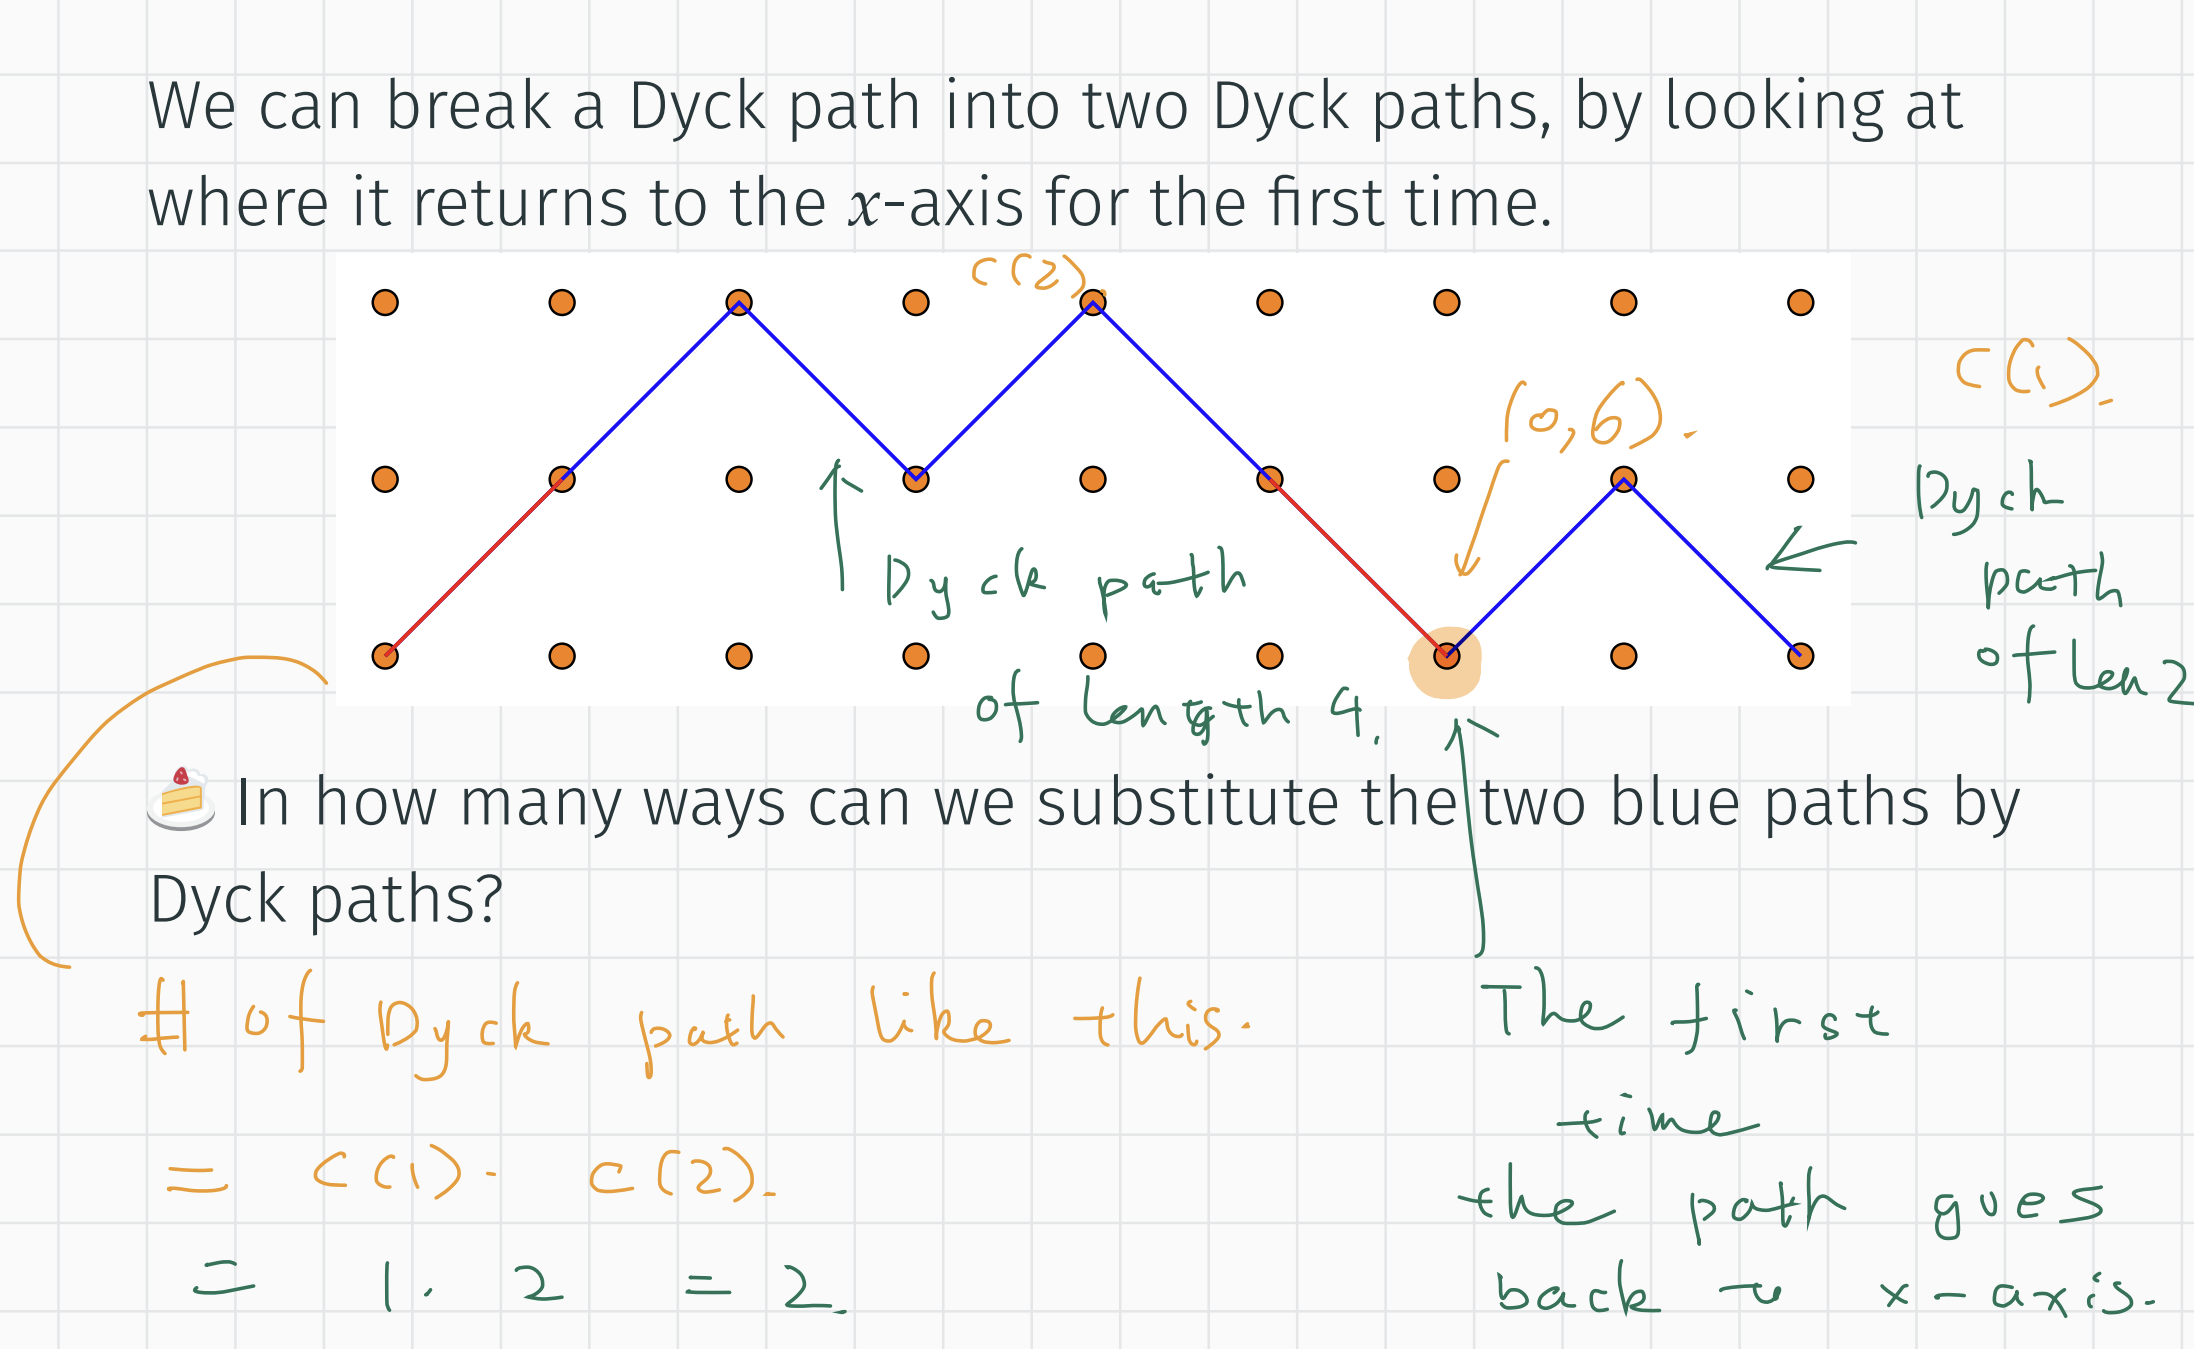
\includegraphics{0002}
$$C(1)*C(2)=2$$ This contributes to a recursion formula $$C_n=\sum_{k=0}^{n-1}C_kC_{n-k-1}$$
\paragraph{Binomial theorem and its implementation}:\newline
$$(x+y)^{n}=\sum_{k=0}^{n}\binom{n}{k}x^ky^{n-k}$$
Example:\newline
the coefficient of $a^{14}b^{18}$ in $(3a^2-5b)^{25}$ is $3^{7}\times 5^{18}\times \binom{25}{7}$\newline
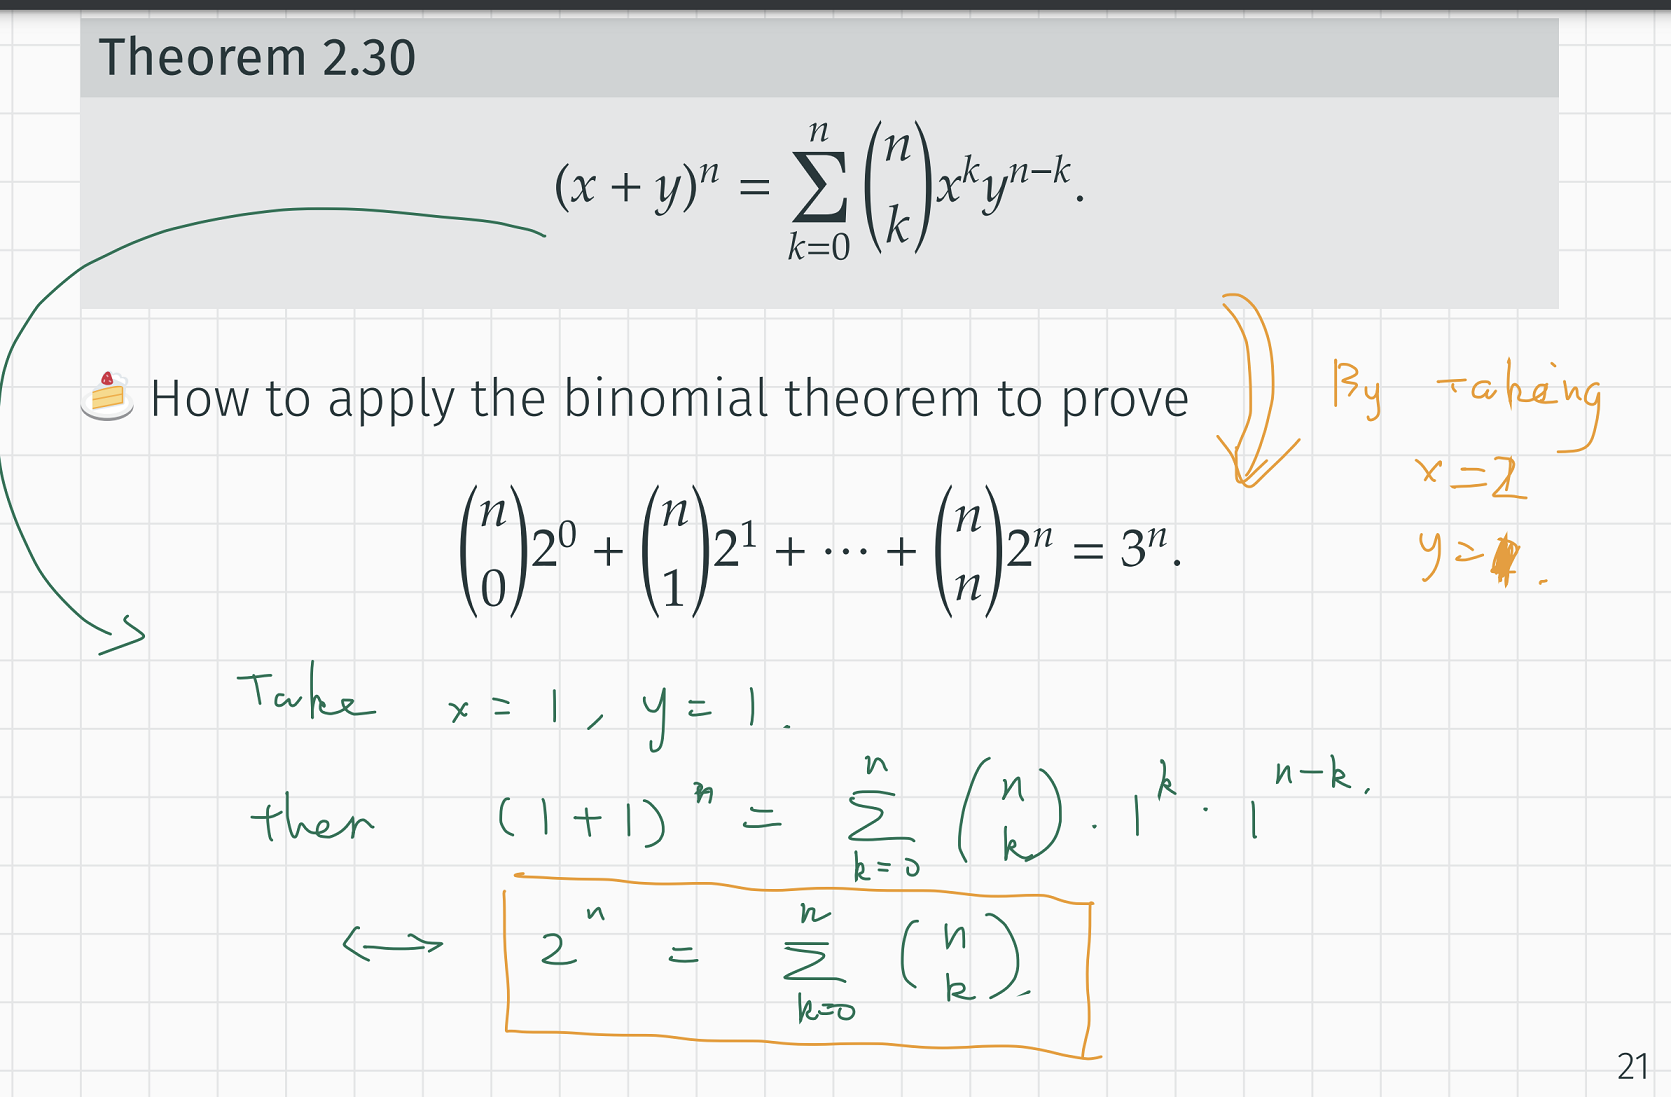
\includegraphics{0003}
\paragraph{Multinomial Coefficients}
Example:\newline
We want n distinct robot with different colors, such that \newline
$k_1$ robots are red\newline
$k_2$ are blue\newline
$k_3=n-k_1-k_2$ are purple\newline
There are 
$$\binom{n}{k_1} \binom{n-k_1}{k_2} \binom{k_3}{k_3}=\frac{n!}{k_1!(n-k_1)!} \frac{(n-k_1)!}{k2!(n-k_1-k_2)!}\cdot 1=\frac{n!}{k_1!k_2!k_3!}$$
choices. \newline
Such numbers are called multinomial coefficients and denoted by
$$\binom{n}{k_1,k_2,\cdots ,k_r}=\frac{n!}{k_1!k_2!\cdots k_r!}$$
Such that
$$(x_1+x_2+\cdots +x_r)^n=\sum_{k_1+k_2+\cdots +k_r=n}\binom{n}{k_1,k_2,\cdots +k_r}x^{k_1}_1 x^{k_2}_2 \cdots x^{k_r}_r$$
\subsubsection{Exercises}
\paragraph{2.9.23}
How many lattice paths are there from (3, 5) to (10, 12)? \newline
Solution:\newline
This problem is equal to how many lattice paths are there from (0,0) to (7,7). Thus, the answer will be:
$$\binom{14}{7}$$
\paragraph{2.9.25}
How many lattice paths from (0, 0) to (17, 12) are there that pass through (7, 6) and
(12, 9)?
\newline
$$\binom{13}{7} \binom{8}{5} \binom{8}{5}$$
\paragraph{2.9.27}A small-town bank robber is driving his getaway car from the bank he just robbed
to his hideout. The bank is at the intersection of 1
st Street and 1
st Avenue. He needs
to return to his hideout at the intersection of 7
th Street and 5
th Avenue. However, one
of his lookouts has reported that the town’s one police officer is parked at the intersection of 4
th Street and 4
th Avenue. Assuming that the bank robber does not want to
get arrested and drives only on streets and avenues, in how many ways can he safely return to his hideout? (Streets and avenues are uniformly spaced and numbered consecutively in this small town.)\newline
Solution:
$$\binom{10}{6}-\binom{6}{3} \binom{4}{3}$$
\paragraph{2.9.29}
Determine the coefficient on $x^{15}y^{120}z^{25}$ in $(2x+3y^2+z)^{100}$\newline
Solution:\newline
$$2^{15}3^{60}\binom{100}{15,60,25}$$
\paragraph{2.9.31}
For each word below, determine the number of rearrangements of the word in
which all letters must be used.\newline
(a) OVERNUMEROUSNESSES \newline
(b) OPHTHALMOOTORHINOLARYNGOLOGY \newline
(c) HONORIFICABILITUDINITATIBUS (the longest word in the English language
consisting strictly of alternating consonants and vowels)\newline
(a) $$\frac{18!}{4!4!2!2!2!2!1!1!}$$
(b)$$\frac{28!}{7!3!3!2!2!2!2!2!2!1!1!1!}$$
(c)$$\frac{27!}{7!3!2!2!2!2!2!}$$
\paragraph{2.9.33}
There are many useful sets that are enumerated by the Catalan numbers. (Volume two of R.P. Stanley’s Enumerative Combinatorics contains a famous (or perhaps infamous) exercise in 66 parts asking readers to find bijections that will show that the
number of various combinatorial structures is C(n), and his web page boasts an additional list of at least 100 parts.) Give bijective arguments to show that each class of
objects below is enumerated by C(n). (All three were selected from the list in Stanley’s
book.) \newline
(a) The number of ways to fully-parenthesize a product of n+1 factors as if the “multiplication” operation in question were not necessarily associative. For example,
there is one way to parenthesize a product of two factors (a1a2), there are two ways
to parenthesize a product of three factors ((a1(a2a3)) and ((a1a2)a3)), and there are
five ways to parenthesize a product of four factors:\newline
(a1(a2(a3a4))), (a1((a2a3)a4)), ((a1a2)(a3a4)), ((a1(a2a3))a4), (((a1a2)a3)a4).\newline
(b) Sequences of n 1’s and n - 1’s in which the sum of the first i terms is nonnegative
for all i.\newline
(c) Sequences $1 \leq a1 \leq \cdots \leq an$ of integers with $ai \leq i$. For example, for n=3, the
sequences are
$$111 112 113 122 123 $$
Solution:\newline
(a) We can show this using a bijection to Dyck paths. An opening bracket is an Up move and a closing
bracket is an Down move.\newline
(b) Again, we can use a bijection to Dyck paths. A “1” corresponds to an Up move and a “-1” corresponds a
Down move.\newline
(c) Subtract one from each number first. Treat the i-th number in the result as the number of boxes below
a lattice path in the i-th column.
\subsection{Lecture 8}
\subsubsection{Course materials}
\paragraph{Sequences}
A sequence is simply an ordered list of infinitely many
numbers. \newline
We can refer whole sequence by
$$(a_n)_{n\in N} \ or \ (a_n)_{n\ge 0}$$
A sequence can be seen as as a function from N to R.
\paragraph{Partial sums}
Given $(a_n)_{n\ge 0}$ we often want to compute the partial sum $$\sum_{i=0}^na_i$$
\paragraph{Induction}
proof by induction:\newline
Let $S_n$ be a statement. To prove $\forall n \in N(S_n)$ is true, we can use induction:\newline
Base case: Show $S_0$ is true.\newline
Induction step:\newline
1.Assume that the statement $S_k$ is true for some integer
$k\ge 0$.\newline
2.Show that $S_{k+1}$ is true.\newline
proof by strong induction:\newline
Let $S_n$ be a statement. To prove $\forall n \in N(S_n)$ is true, we can use induction:\newline
Base case: Show $S_0$ is true.\newline
Induction step:\newline
1.Assume that the statement $S_k$ is true for all
$k\ge 0$ for some integer n.\newline
2.Show that $S_{k+1}$ is true.\newline
Strong induction and induction are logically equivalent. But
sometimes the strong version is a bit more convenient.
\subsubsection{Exercises: Applied Combinatorics (AC)}
\paragraph{3.9.5}
Let S be the set of strings on the alphabet {0, 1, 2, 3} that do not contain 12 or 20 as
a substring. Give a recursion for the number h(n) of strings in S of length n.\newline
Solution:\newline
$$h(n)=4h(n-1)-2h(n-2)+h(n-3),h(1)=4,h(2)=14,h(3)=49$$
Our recursion
involves looking back 3 terms,(h(n-3)) so we need specify 3 initial values. Valid strings
of length n can be formed as follows. Take a valid string of length n-1, and place a 0 or 3
in the front. Since the last n-1 positions do not contain a 12, placing a 0 or a 3 in the first
position preserves this property, and so there are 2h(n-1) valid length n strings starting with
a 0 or a 3. We can also place a 1 or a 2 in the first position, but then we must subtract out
the length n-1  strings that have a 2 or a 0 in their first position respectively. The number of
valid length n-1 strings that have a 2 in the first position is $h(n-2)-h(n-3)$ – it would
be h(n-2) but we cannot have a 0 afterward so we subtract out h(n-3) such strings – and
hence, the number of valid length n strings starting with a 1 is $h(n-1)-(h(n-2)-h(n-3))$. The number of valid length n-1 1 strings that have a 0 in the first position is h(n-2) Hence,
the number of valid length n strings starting with a 2 is h(n-1) -h(n-2) Adding these
disjoint cases together gets the result.
\paragraph{3.9.7}
Find gcd(827, 249) as well as integers a and b such that $827a + 249b=6$\newline
Solution:\newline
gcd(827, 249) = gcd(249, 827 mod 249) = gcd(249, 178) = gcd(178, 249 mod 178) = gcd(178, 71) = gcd(71, 178 mod 71) = gcd(71, 107) = gcd(107, 71) = gcd(71, 107 mod 71) = gcd(71, 36) = gcd(36, 71 mod 36) = gcd(36, 35) = gcd(35, 36 mod 35) = gcd(35, 1) = 1 \newline
Therefore, the gcd of 827 and 249 is 1. \newline
Since the gcd of 827 and 249 is 1, it follows that there exist integers a and b such that 827a + 249b = 1. Multiplying both sides of this equation by 6, we get:\newline
827 * 6a + 249 * 6b = 6\newline
So, a = -10, b = 43 is a solution to the equation 827a + 249b = 6.
Standard solution:\newline
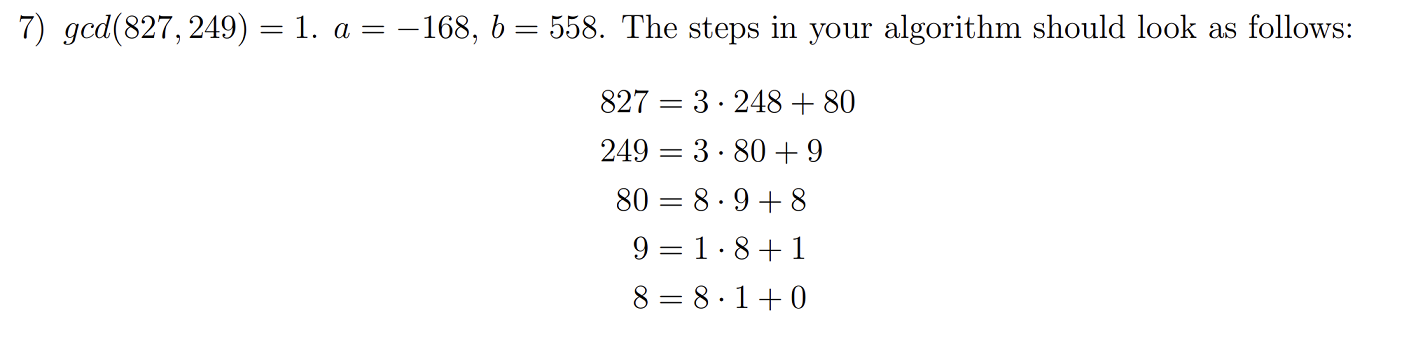
\includegraphics{0008}
\paragraph{3.9.9}(A challenging problem) For each formula, give both a proof using the Principle of
Mathematical Induction and a combinatorial proof. One of the two will be easier while
the other will be more challenging \newline
(a)$$1^2+2^2+3^2+\cdots +n^2=\frac{n(n+1)(2n+1)}{6}$$
(b)$$\binom{n}{0}2^0+\binom{n}{1}2^1+\cdots +\binom{n}{n}2^n=3^n$$
(a) The base case:\newline
$$1^2=\frac{1(1+1)(2\cdot 1+1)}{6}$$
For the inductive step, use the inductive hypothesis to conclude:
$$1^2+2^2+\cdots (n-1)^2+n^2=\frac{(n-1)(n)(2(n-1)+1)}{6}+n^2$$
Basic algebraic manipulations show that the right hand side is equal to $\frac{n(n+1)(2n+1)}{6}$ For a
combinatorial proof, both sides count the number of 3-tuples (x, y, z) where $0\leq x,y<z\leq n$ On the left hand side, if $z=k$ there are $k^2$ choices for x and y – they can each be any number $0,1,\cdots k-1$. Summing up these cases gives the left hand side. For the right hand
side, we divide the problem into two cases.\newline
Case 1: We first consider such triples where x = y. There are $\binom{n+1}{2}$ such triples since we choose 2 distinct elements from $\{0,1,\cdots ,n\}$ , let the larger number be z and the smaller number be x and y.
Case 2:  If x < y, then there are $\binom{n+1}{3}$ such triples. If x $>$ y, there are also $\binom{n+1}{3}$ such triples. Basic algebraic manipulation shows that:
$$\binom{n+1}{2}+2 \binom{n+1}{3}=\frac{n(n+1)(2n+1)}{6}$$
(b)Combinatorial proof:\newline
RHS: $3^n$ is the amount of ternary string (e.g.\{"0","1","2"\}) of length n.\newline
LHS: $\binom{n}{k}\cdot 2^k$ is the amount of ternary string containing "0", "0" ($\binom{n}{k}$ means k positions out of n positions) ($2^k$ means the amount of the binary string). While n-k means it does not contain "0","0". We add them up,then we can get the amount of the ternary string.\newline
Therefore, LHS=RHS.\newline
of. For the inductive proof, we will use Pascal’s formula which we recall for the reader:
$$\binom{n}{k}=\binom{n-1}{k-1}+\binom{n-1}{k}$$
Now, for the base case,
$$\binom{1}{0}2^0+\binom{1}{1}2^1=1+2=3^1$$
For the inductive step,
$$\sum_{k=0}^{n}\binom{n}{k}2^k=\binom{n}{0}+\sum^{n-1}_{k=1}(\binom{n-1}{k-1}+\binom{n-1}{k})\cdot 2^k+\binom{n}{n}2^n$$
$\Longrightarrow$
$$1+2\sum_{k=1}^{n-1}\binom{n-1}{k-1}2^{k-1}+\sum_{k=1}^{n-1}\binom{n-1}{k}2^k+1$$
$\Longleftarrow$
$$2\cdot 3^{n-1}+3^{n-1}=3^n$$
\paragraph{3.9.11}
Show that for all positive integers n,
$$\sum_{i=0}^{n}2^i=2^{n+1}-1$$\newline
Solution:\newline
1) We show this by induction. For the base case of $n=0,2^0=1=2^{0+1}-1$. For the inductive step,
$$\sum_{i=0}^{n}=2^n+\sum_{i=0}^{n-1}2^i=2^n+2^n-1=2^{n+1}-1$$
\paragraph{3.9.13}
Show that for all positive integers $n,9^n-5^n$ is divisible by 4.\newline
For $n=1,9-5=4$. For the inductive step,
$$9^n-5^n=9\cdot 9^{n-1}-5\cdot 5^{n-1}=4\cdot 9^{n-1}+5(9^{n-1}-5^{n-1})$$
,By the induction hypothesis, $9^{n-1}-5^{n-1}=4k$ for some positive integer k. Hence, $$9^n-5^n=4(9^{n-1}+5k)$$
\paragraph{3.9.15}Use mathematical induction to prove that for all integers $n\ge 1$,\newline
$$n^3+(n+1)^3+(n+2)^3$$ is divisible by 9.\newline
Solution:\newline
For n=1:
$$1^3+2^3+3^3=1+8+27=36=4\cdot 9$$
. For the inductive step, first observe that
$$(n-1)^3=n^3-3n^2+3n-1$$
Now,
$$n^3+(n+1)^2+(n+2)^3=n^3+(n+1)^3+n^3+6n^2+12n+8$$
$\Longrightarrow$
$$n^3+(n+1)^3+n^3-3n^2+3n-1+9n^2+9n+9$$
$\Longrightarrow$
$$(n-1)^3+n^3+(n+1)^3+9n^2+9n+9$$
By the induction hypothesis, the sum of the first 3 terms is divisible by 3. The last 3 terms
are obviously divisible by 3, and so this proves the statement.
\paragraph{3.9.17}Consider the recursion given by $f(n)=2f(n-1)-f(n-2)+6$ for $n \ge 2$ with $f(0)=2$ and $f(1)=4$. Use mathematical induction to prove that $f(n)=3n^2-n+2$ for all integers $n\ge 0$.\newline
Solution:\newline
For $n=0$,$3\cdot 0^2-0+2=2=f(0)$, and for n=1, $3\cdot 1^2-1+2=4=f(1)$
For the inductive step, since
$$f(n)= 2f(n - 1) - f(n - 2) + 6$$,
we may apply the inductive hypothesis (we use strong induction here) to conclude
$$f(n)=2(3(n-1)^2-(n-1)+2)-(3(n-2)^2-(n-2)+2)+6$$
Basic algebraic manipulations show that this is equal.\newline
$$3n^2-n+2$$
\paragraph{3.9.19}
Suppose $x\in R$ and $x>-1$. Prove that for all integers $n\ge 0$, $$(1+x)^n\ge 1+nx$$.\newline
Solution:\newline
For n=0, $(1+x)^0=1 \ge 1 +0\cdot x=1$. For the inductive step,
$$(1+x)^n=(1+x)(1+x)^{n-1}\ge (1+x)(1+(n-1)x)$$
$\Longrightarrow$
$$1+(n-1)x+x+(n-1)x^2$$
$\Longrightarrow$
$$1+nx+(n-1)x^2\ge 1+nx$$
\subsubsection{Exercises: Discrete Mathematics}
\paragraph{2.5.11}
Prove that the sum of the interior angles of a convex n-gon is $(n-2)\cdot 180^{\circ}$.
(A convex n-gon is a polygon with n sides for which each interior
angle is less than $180^{\circ}$
.)\newline
Hint:\newline
Start with (k + 1)-gon and divide it up into a k-gon and a triangle.\newline
Solution:\newline
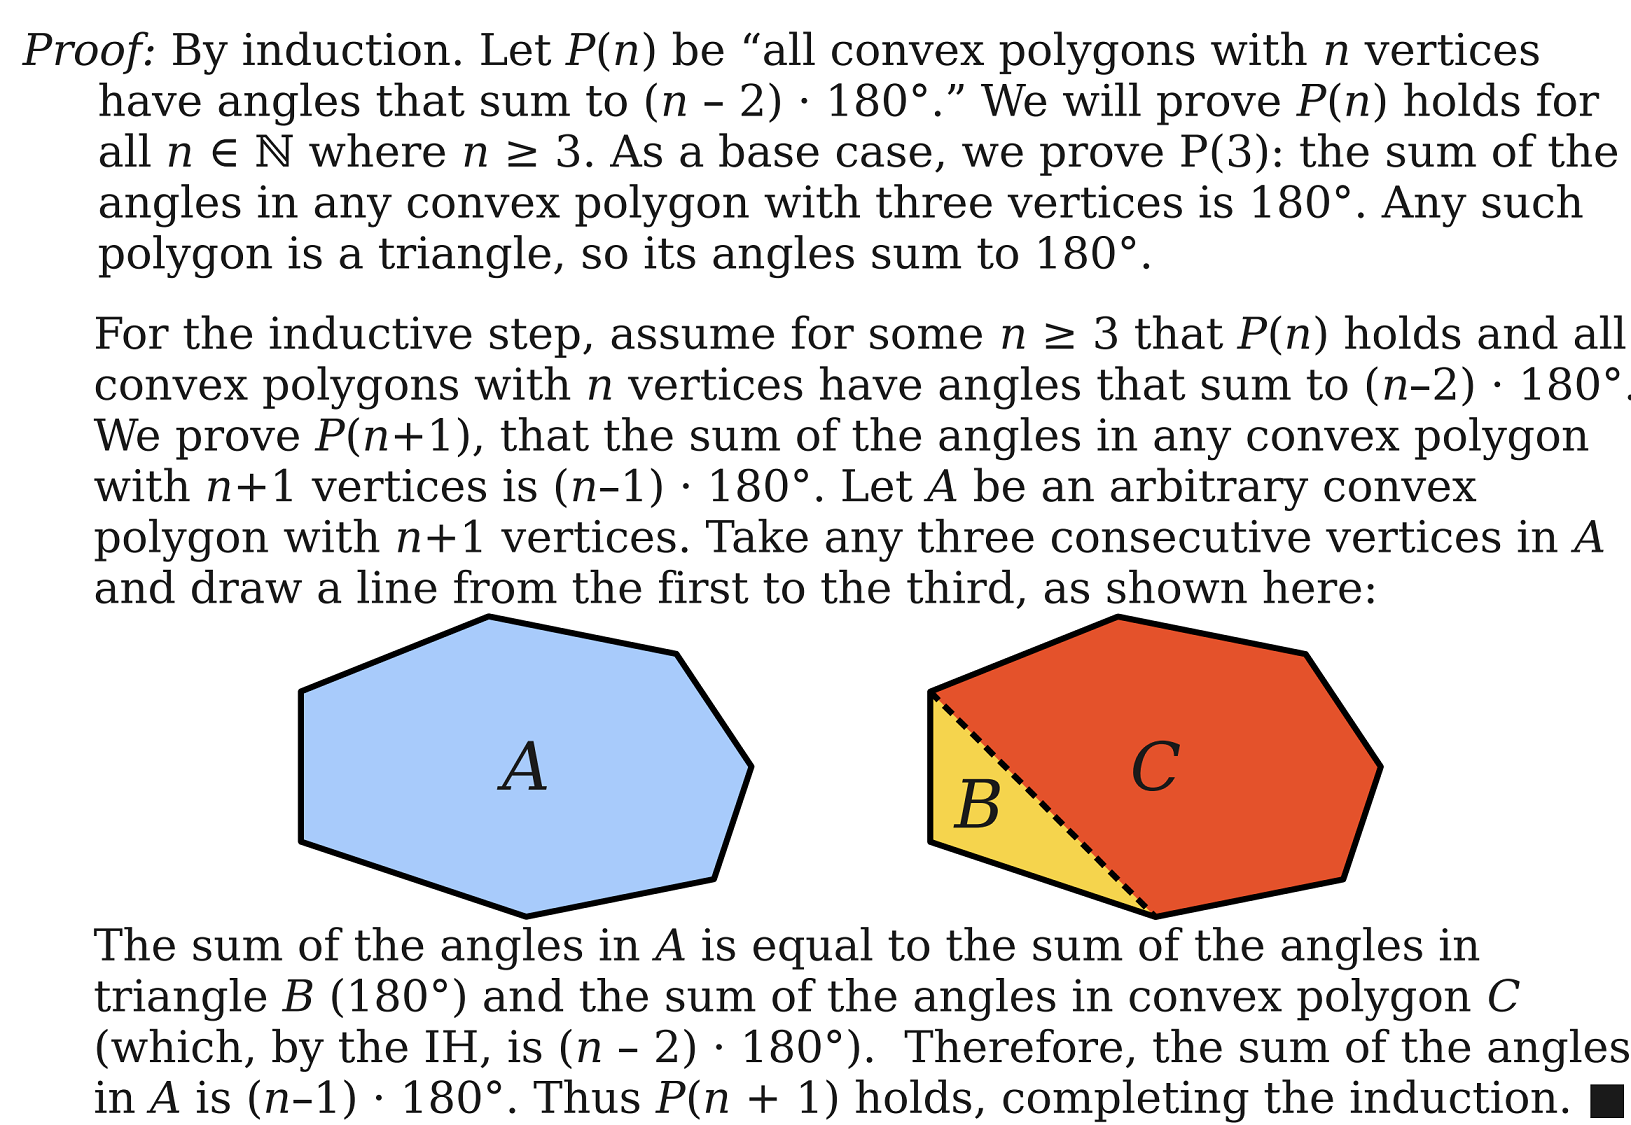
\includegraphics{0010}
\paragraph{2.5.29}
Given a square, you can cut the square into smaller squares by cutting
along lines parallel to the sides of the original square (these lines do
not need to travel the entire side length of the original square)example, by cutting along the lines below, you will divide a square
into 6 smaller squares:\newline
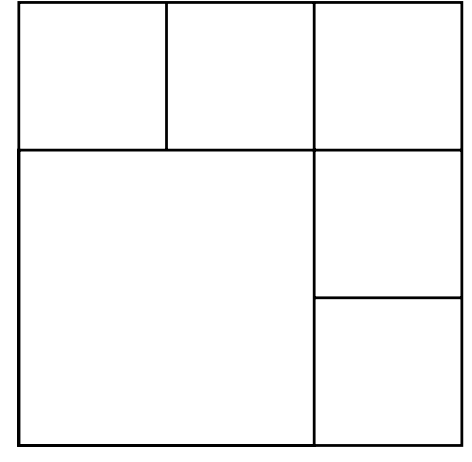
\includegraphics{0009}\newline
Prove, using strong induction, that it is possible to cut a square
into n smaller squares for any $n\ge 6$.\newline
Hint:\newline
You will need three base cases. This is a very good hint actually, as
it suggests that to prove P(n) is true, you would want to use the fact that
P(n - 3) is true. So somehow you need to increase the number of squares
by 3.\newline
solution (by chatGPT):\newline
To prove that it is possible to cut a square into $n$ smaller squares for any $n \ge 6$, we can use strong induction with three base cases.
\newline
Base case 1: $n = 6$. This has been demonstrated in the example given.
\newline
Base case 2: $n = 7$. Draw a diagonal line through one of the squares of the 6 smaller squares. This will divide the square into two smaller squares, one of which is the square we started with. This means that we now have 7 smaller squares.
\newline
Base case 3: $n = 8$. Draw two diagonal lines through two adjacent squares of the 6 smaller squares. This will divide each of the two squares into two smaller squares. This means that we now have 8 smaller squares.
\newline
Inductive step: Assume that it is possible to cut a square into $k$ smaller squares for any $6 \le k \le n$. We will show that it is possible to cut a square into $n + 3$ smaller squares.
\newline
Divide the square into $(n-3)$ smaller squares as per the induction hypothesis. Then draw three diagonal lines through three adjacent squares. The diagonal lines will divide each of the three squares into two smaller squares. This means that we now have $n + 3$ smaller squares.
\newline
By induction, it follows that it is possible to cut a square into $n$ smaller squares for any $n \ge 6$.
\newpage \section{Week3}
\subsection{Lecture 9}
\subsubsection{Course materials}
\paragraph{The number of CS students}:\newline
Let X be the set of 63 students in a discrete math course.
Suppose there are 47 computer science majors and 51 male
students.
Also, we know there are 45 male students majoring in computer
science. \newline
How many students in the class are female students not
majoring in computer science?\newline
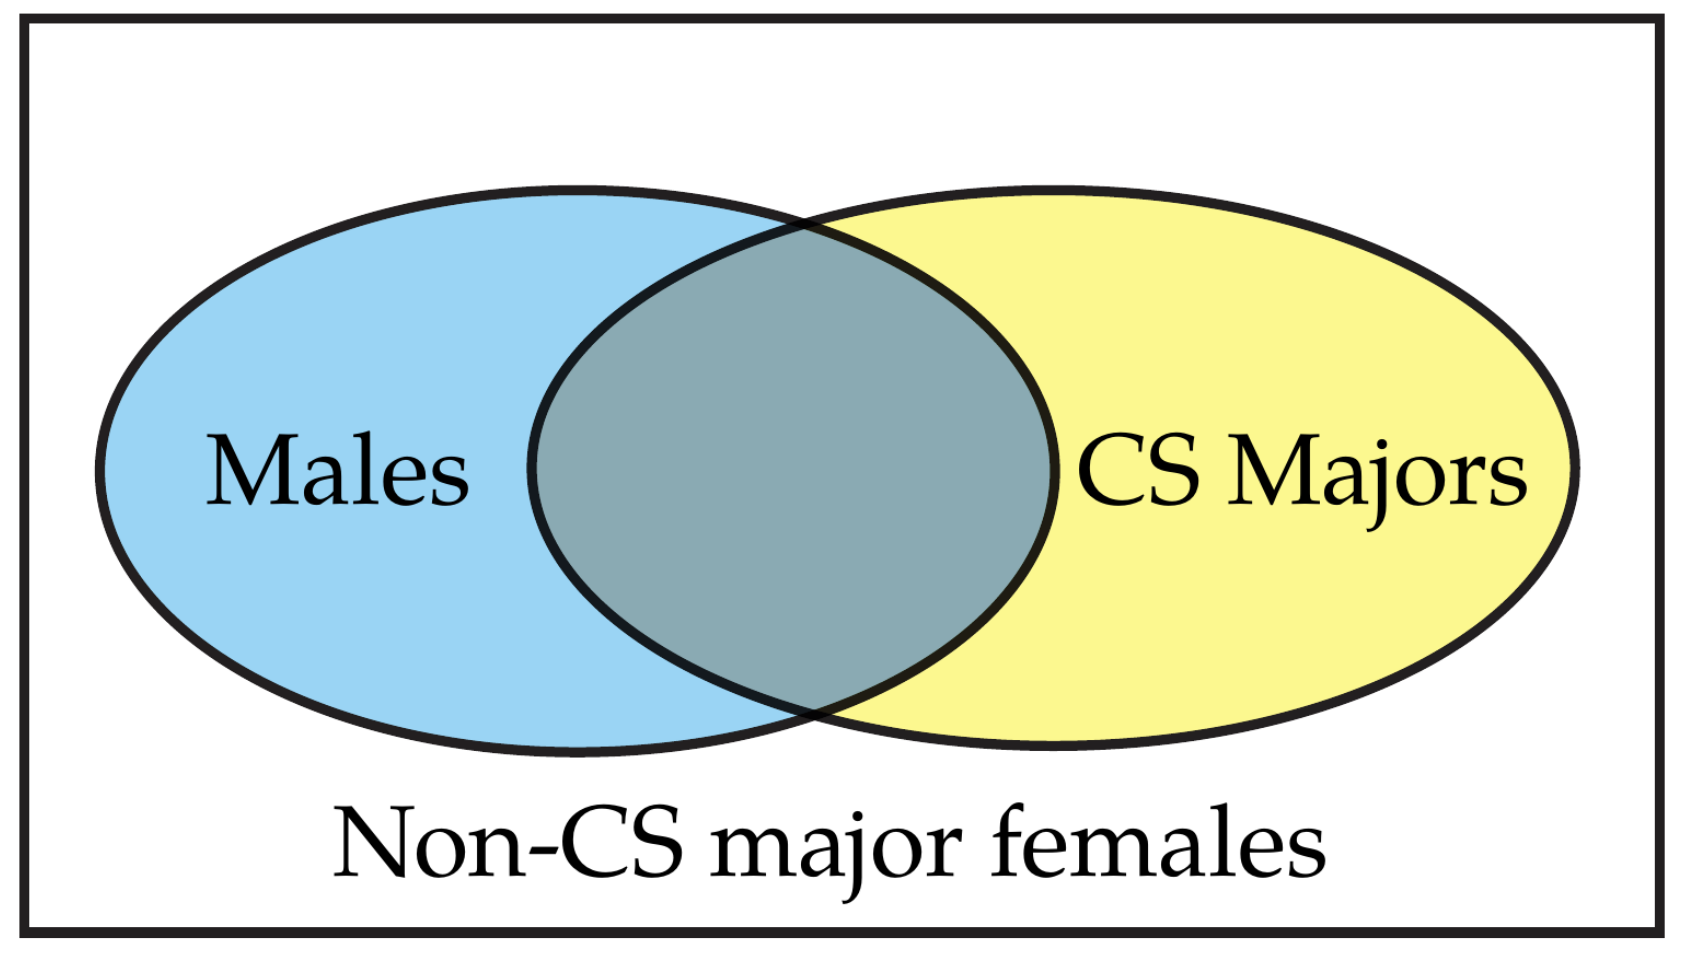
\includegraphics{0004}\newline
Males:51; CS Majors:47; $Males \land CS \ Majors=45$\newline
Solution:\newline
$N=X-Males-CS \ Majors +Males \land CS \ Majors=63-51-47+45=10$
\paragraph{Integer solutions}:\newline
What is the number integer solutions for $x_1+x_2+x_3+x_4=97$ with $x_1,x_2,x_3,x_4 \ge 0, x_3 \leq 7, x_4 \leq 8$ ?\newline
Simplified:\newline
1)$x_1+x_2+x_3+x_4=97$ with $x_1,x_2,x_3,x_4 \ge 0$ contributes to $\binom{97+4-1}{4-1}$ \newline
2)$x_1+x_2+x_3+x_4=97$ with $x_1,x_2,x_3,x_4 \ge 0$ with $x_3>7$ is $\binom{97+3-1-7}{4-1}$ \newline
3)$x_1+x_2+x_3+x_4=97$ with $x_1,x_2,x_3,x_4 \ge 0$ with $x_4>8$ is $\binom{97+3-1-8}{4-1}$ \newline
4)$x_1+x_2+x_3+x_4=97$ with $x_1,x_2,x_3,x_4 \ge 0$ with $3_3>7,x_4>8$ is $\binom{97+2-1-8-7}{4-1}$ \newline
5) Thus, the answer will be $$\binom{97+4-1}{4-1}-\binom{97+3-1-7}{4-1}-\binom{97+3-1-8}{4-1}+\binom{97+2-1-8-7}{4-1}$$
A better idea for 2) is change the question to $x_1+x_2+x_3+x_4=97$ with $x_1,x_2,x_3,x_4 \ge 0$ with $x_3 \ge 8$ is $\binom{97-8+4-1}{4-1}$\newline
A better idea for 3) is change the question to $x_1+x_2+x_3+x_4=97$ with $x_1,x_2,x_3,x_4 \ge 0$ with $x_4 \ge 9$ is $\binom{97-9+4-1}{4-1}$\newline
\paragraph{Principle of inclusion-exclusion}:\newline
Some notations:\newline
For  a subset $S\subseteq [m]$, let N(s) denote the number of elements of X which satisfy property $P_i$ for all $i\in S$.
Theorem 7.7 \newline
The number of elements of X which satisfy none of the
properties in $P = \{p_1,p_2,\cdots,p_m\}$is given by $$\sum_{Y\subseteq [m]}(-1)^{|Y|}N(Y)$$,
where $[m]=\{1,2,\cdots ,m\}$.\newline
1) Proof by induction.\newline
2) What is it when m=1 or m=2.\newline
When m=1:\newline
$$\sum_{Y\subseteq [1]}(-1)^{|Y|}N(Y)=|x|-N(\{1\})$$
\paragraph{The number of surjections}
The number S(n,m) of surjections from [n] to [m] is given by:$$S(n,m)=\sum_{k=0}^m(-1)^k\binom{m}{k}(m-k)^n$$
Proof of Inclusion-Exclusion:\newline
The proof of $$\sum_{Y\subseteq [m]}(-1)^{|Y|}N(Y)$$ is by induction.\newline
Proof - The base case is m=1.\newline
Assume that the equation holds for m=k where $k\ge 1$. Now
consider $m=k+1$.\newline
Split X into\newline
1) $X'$ - elements of X which satisfies $P_{k+1}$\newline
2) $X''$ - elements of X which does not satisfy $P_{k+1}$\newline
Then apply the induction hypothesis to both sets.
\subsubsection{Exercises}
\paragraph{7.7.1}
A school has 147 third graders. The third grade teachers have planned a special treat for the last day of school and brought ice cream for their students. There are three flavors: mint chip, chocolate, and strawberry. Suppose that 60 students like (at least) mint chip, 103 like chocolate, 50 like strawberry, 30 like mint chip and strawberry, 40 like mint chip and chocolate, 25 like chocolate and strawberry, and 18 like all three flavors. How many students don’t like any of the flavors available? \newline
Solution:\newline
Answer=147-60-103-50+30+30+25-18=11
\paragraph{7.7.3}
How many positive integers less than or equal to 100 are divisible by 2? How many
positive integers less than or equal to 100 are divisible by 5? Use this information to
determine how many positive integers less than or equal to 100 are divisible by neither
2 nor 5.\newline

40. There are 50 positive integers less than or equal to 100 that are divisible by 2. They
are $\{2 \cdot k : k = 1, \cdots , 50\}$. There are 20 positive integers less than or equal to 100 that are
divisible by 5. They are $\{5 \cdot k : k = 1,  20\}$. Let A be the first set and B be the second
set. If we can determine $A \cup B$, then the number of positive integers less than or equal to 100
that are not divisible by 2 or 5 will be $100 - |A \cup B|$.
\paragraph{7.7.5}
How many positive integers less than or equal to 1000 are divisible by none of 3, 8,
and 25?\newline
Solution:\newline
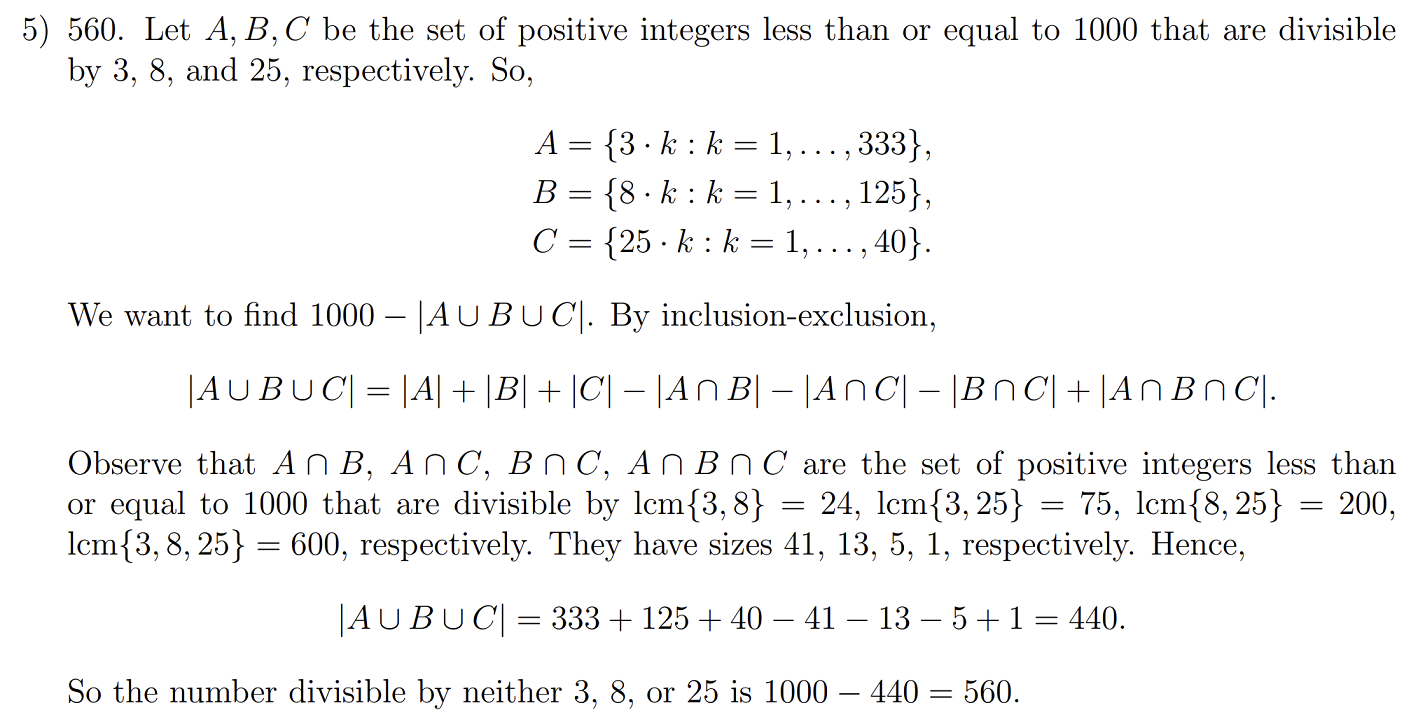
\includegraphics{0011}
\paragraph{7.7.7}
How many integer solutions are there to the equation $x1 + x2 + x3 + x4 = 32$ with
$0 \leq x_i \leq 10$ for $i = 1, 2, 3, 4$?\newline
Solution:\newline
The number of solutions of $x1 + x2 + x3 + x4 = 32$ without solution is that $\binom{32+4-1}{4-1}$. Let $A_i$ denote the set of the solutions $x1 + x2 + x3 + x4 = 32$ with $x_i\ge 10$. Therefore, the number of solutions will be$$\binom{35}{3}-|A_1\cup A_2\cup A_3 \cup A_4|$$
Hence, we use inclusion-exclusion to determine the size of the union of the $A_i$
$$|A_i|=\binom{24}{3}$$
$$|A_i\cap A_j|=\binom{13}{3}$$
$$|A_i\cap A_j \cap A_k|=0$$
$$|A_1\cap A_2 \cap A_3 \cap A_4|=0$$ Hence,
$$|A_1\cup A_2\cup A_3 \cup A_4|=4\binom{13}{3}-6\binom{24}{3}$$
Therefore, the number of solutions will be
$$\binom{35}{3}-[4\binom{13}{3}-6\binom{24}{3}]$$
\paragraph{7.7.9}
A graduate student eats lunch in the campus food court every Tuesday over the
course of a 15-week semester. He is joined each week by some subset of a group of
six friends from across campus. Over the course of a semester, he ate lunch with each
friend 11 times, each pair 9 times, and each triple 6 times. He ate lunch with each group of four friends 4 times and each group of five friends 4 times. All seven of them
ate lunch together only once that semester. Did the graduate student ever eat lunch
alone? If so, how many times?\newline
Solution:\newline
Yes, he ate alone 1 time. Label his friends 1, 2, 3, 4, 5, 6, and let $A_i$ be the set of weeks that
he ate lunch with friend $i$. Since there are 15 weeks in the semester, the number of times he
ate alone is $$15-|\bigcup_{i=1}^6 A_i|$$
By inclusion-exclusion, the size of the union is
$$|\bigcup_{i=1}^6 A_i|=\sum_{i=1}^6|A_i|-\sum|A_i\cap A_j|+ \cdots -|A_1\cap A_2 \cap \cdots \cap A_6|$$
The problem statement gives us the size of each of these intersections, so $$|\bigcup_{i=1}^6 A_i|=6\cdot 11-\binom{6}{2}\cdot 9 +\binom{6}{3}\cdot 6 - \binom{6}{4}\cdot 4 +\binom{6}{5}\cdot 4 -1=14$$
So, he ate alone $15 - 14 = 1$ time.
\paragraph{7.7.11}
As in Example 7.4, let X be the set of functions from [n] to [m] and let a function
$f \in X$ satisfy property $P_i$
if there is no j such that $f (j) = i$.\newline
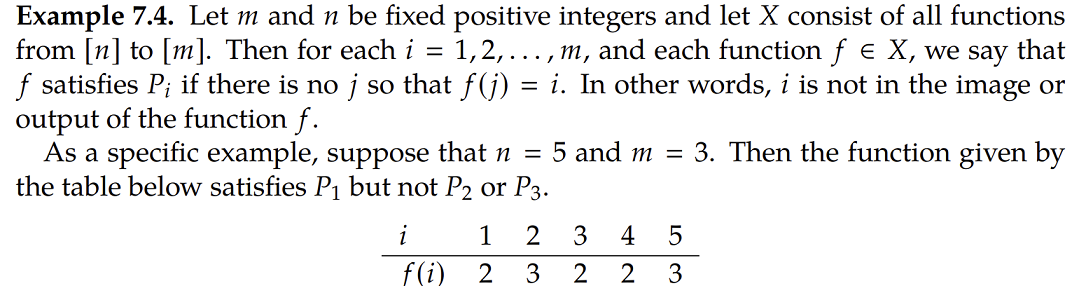
\includegraphics{Example7.4}\newline
(a) Let the function $f : [8] \to [7]$ be defined by Table 7.18. Does f satisfy property
$P_2$? Why or why not? What about property $P_3$? List all the properties $P_i$ (with
$i \leq 7$) satisfied by f.\newline
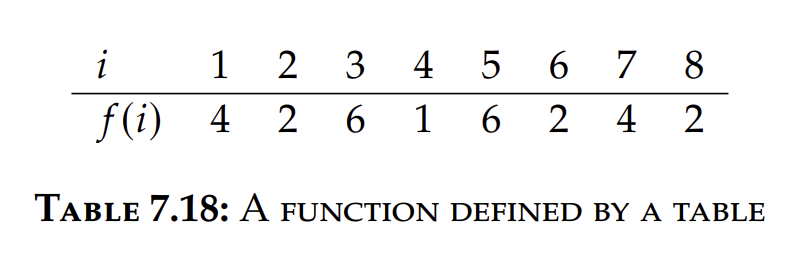
\includegraphics{Table7.18}\newline
(b) Is it possible to define a function 1 : $[8] \to [7]$ that satisfies no property $P_i$
, $i \leq 7$?
If so, give an example. If not, explain why not.\newline
(c) Is it possible to define a function h : $[8] \to [9]$ that satisfies no property $P_i$
, $i \leq 9$?
If so, give an example. If not, explain why not.\newline
Solution:\newline
(a). No, because f(2) = 2 (and also f(6) = 2). Yes, it satisfies $P_3$. It also satisfies $P_5$ and $P_7$.\newline
(b). Yes. Let g(x) = x for 1 $\leq$ x $\leq$ 7 and g(8) = 1. Then g satisfies no $P_i$
for i $\leq$ 7.
(c). No, it is not possible because since 9 $>$ 8, there will always be an element in $\{1, 2, . . . , 9\}$
that does not get mapped to by h.
\paragraph{7.7.13}
As in Example 7.6, let m and n be positive integers and X=[n]. Say that j $\in$ X
satisfies property $P_i$ for an i with 1 $\leq$ i $\leq$ m if i is a divisor of j.\newline
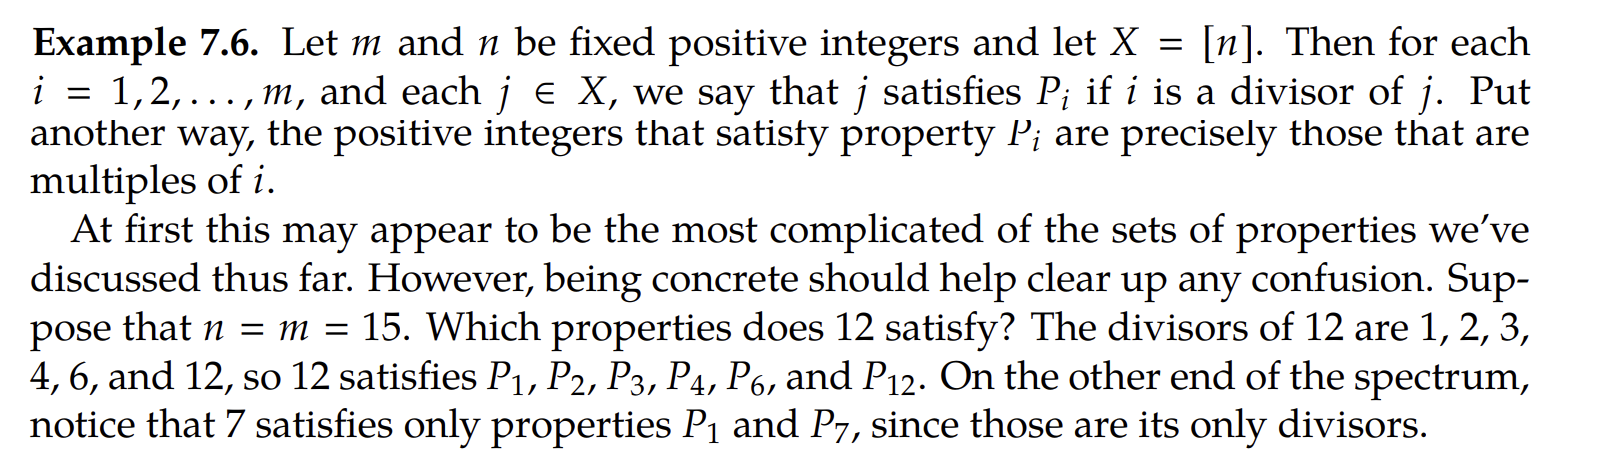
\includegraphics{Example7.6}\newline
(a) Let m = n = 15. Does 12 satisfy property $P_3$? Why or why not? What about
property $P_5$? List the properties $P_i$ with 1 $\leq$ i $\leq$ 15 that 12 satisfies.\newline
(b) Give an example of an integer j with 1 $\leq$ j $\leq$ 15 that satisfies exactly two properties $P_i$ with 1 $\leq$ i $\leq$ 15.\newline
(c) Give an example of an integer j with 1 $\leq$ j $\leq$ 15 that satisfies exactly four properties $P_i$ with 1 $\leq$ i $\leq$ 15 or explain why such an integer does not exist.\newline
(d) Give an example of an integer j with 1 $\leq$ j $\leq$ 15 that satisfies exactly three properties $P_i$ with 1 $\leq$ i $\leq$ 15 or explain why such an integer does not exist.\newline
Solution:\newline
(a). Yes, because 12 $\in$ [15] and 3 divides 12. It does not satisfy $P_5$ since 5 does not divide
12. It also satisfies $P_1$, $P_2$, $P_4$, $P_6$, $P_{12}$.\newline
(b). 2 satisfies only $P_1$ and $P_2$. Any other prime will also work.\newline
(c). 6 satisfies $P_1$, $P_2$, $P_3$, $P_6$.\newline
(d). 4 satisfies $P_1$, $P_2$, $P_4$.
\paragraph{7.7.15}
A teacher has 10 books (all different) that she wants to distribute to John, Paul,
Ringo, and George, ensuring that each of them gets at least one book. In how many
ways can she do this?\newline
Solution:\newline
S(10, 4). This is equal to the number of surjections from a set of 10 elements (the books) to
a set of 4 elements (John, Paul, Ringo, and George). Since we are counting surjections, this
means that each of them will get at least one book.
\paragraph{7.7.17}
A professor is working with six undergraduate research students. He has 12 topics
that he would like these students to begin investigating. Since he has been working
with Katie for several terms, he wants to ensure that she is given the most challenging
topic (and possibly others). Subject to this, in how many ways can he assign the topics
to his students if each student must be assigned at least one topic?\newline
Solution:\newline
S(11, 5)+S(11, 6). Label the students with elements from [6], and label the topics with labels
from [12]. Let Katie be labeled 6, and let the hardest topic be labeled 12. The number of ways
that the professor can assign topics is the number of mappings from [12] to [6] such that the
map is a surjection and 12 gets mapped to 6. If Katie does not receive any extra topics, then
this is equal to the number of surjections from [11] to [5] which is S(11, 5). If Katie receives
some extra topics, then this is equal to the number of surjections from [11] to [6] which is
S(11, 6). Since these cases are disjoint, their sum gives us the total number of mappings.
\subsection{Lecture 10}
\subsubsection{Course material}
\paragraph{Derangement-Hat problem}
Suppose that 20 Swedish students get very excited in their graduation ceremony and throw their hat into the air.\newline
Each student gets a hat back uniformly at random.\newline
What is the probability that no one gets his/her own hat back.\newline
Previous knowledge: Permutation \newline
A permutation can be seen as a surjective function from [n] to [n].\newline
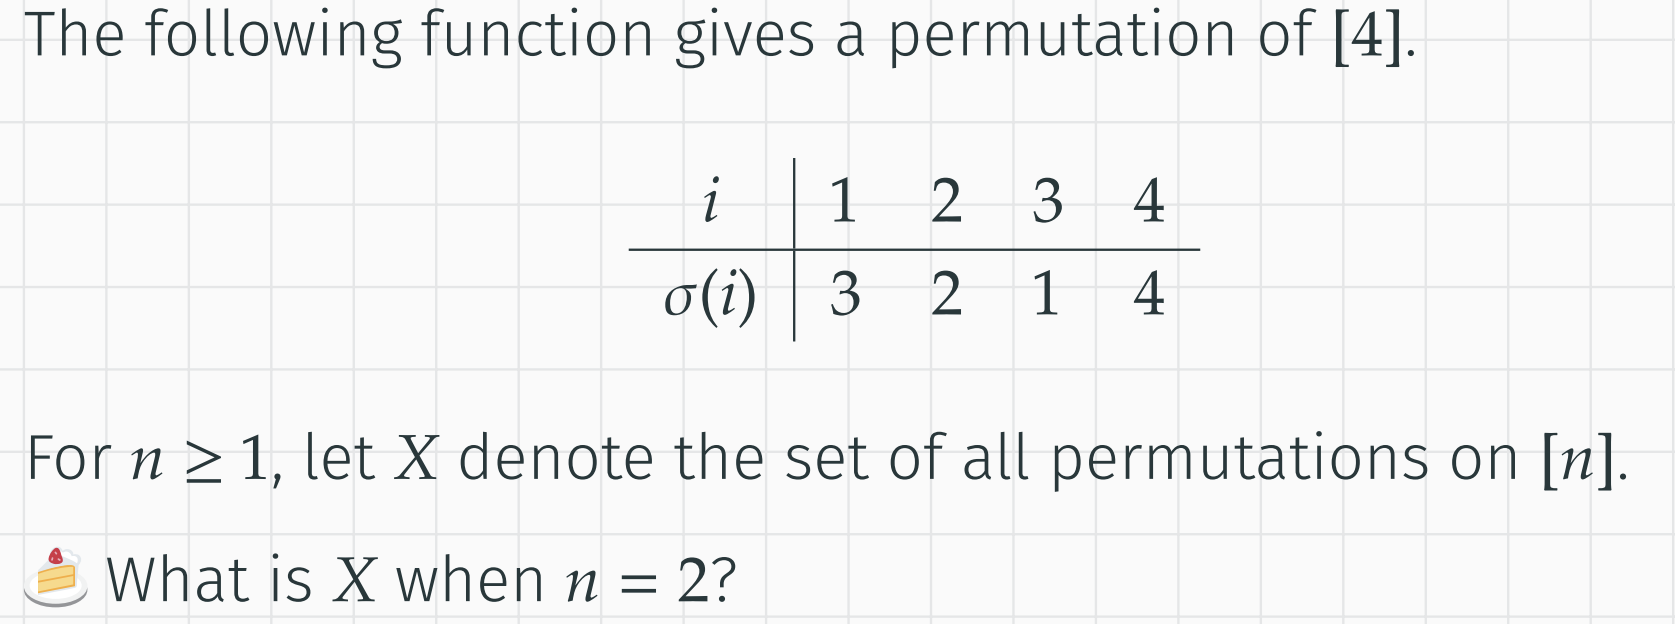
\includegraphics{0005}\newline
When n=2, $X=\{12,21\}$
Therefore, there comes derangement.\newline
Derangement:\newline
A permutation $\sigma \in X$ is called a derangement if $\sigma (i) \neq i$ for all $i\in [n]$\newline
To calculate derangement, here comes an example:\newline
Count N(S) when n=5:\newline
1) Fix 1, we have 4 positions left. Such that we have 4!.\newline
2) Fix 2, we have 4 positions left. Such that we have 4!. \newline
$$\cdots $$
5) Fix 5, we have 4 positions left. Such that we have 4!. \newline
12) Fix 1 and 2, we have 3 positions left. Such that we have 3!.
$$\cdots$$
12345) All fixed, we have 1!.\newline
Therefore, we can find that:\newline
For each subset $S\subseteq [n] \ with \ |S|=k$, we have $$N(S)=(n-k)!$$
Thus, to count derangements: we have \newline
For each positive integer  n, the number $d_n$ of derangements of [n] satisfy $$d_n=\sum^{n}_{k=0}\binom{n}{k}(n-k)!$$
Proof: The inclusion-exclusion. \newline
$$\sum_{Y\subseteq [m]}(-1)^{|Y|}N(Y)$$
$\Longrightarrow$
$$\sum_{k=0}^{n}\sum_{Y\subseteq [n],Y=|k|}(-1)^{|Y|}N(Y)$$
$\Longrightarrow$
$$\sum_{k=0}^{n}\sum_{Y\subseteq [n],Y=|k|}(-1)^{k}(n-k)!$$
$\Longrightarrow$
$$\sum_{k=0}^{n}(-1)^{k}(n-k)!\sum_{Y\subseteq [n],Y=|k|}1$$
$\Longrightarrow$
$$\sum_{k=0}^{n}(-1)^{k}(n-k)!\binom{n}{k}$$
Thus, the answer of the hat problem is
$$\frac{d_{20}}{20!}$$
$20!$ is the number of permutation of 20.
\paragraph{The Limit}
For a positive integer n, let $d_n$ denote the number of derangement of [n]. Then
$$\lim_{n\to \infty}\frac{d_n}{n!}=\frac{1}{e}$$
Recall from calculus that by definition
$$e^x=\lim_{n\to \infty} \sum_{i=i}^{n}\frac{x^i}{i!}$$
$$\frac{dn}{n!}=\sum_{k=0}^n(-1)^k\binom{n}{k}\frac{(n-k)!}{n!}=\sum_{k=0}^n(-1)^k\frac{n!}{k!(n-k)!}\cdot \frac{(n-k)!}{n!}$$
$\Longrightarrow$
$$\sum_{k=0}^n(-1)^k\cdot \frac{1}{k!}\to \frac{1}{e}$$
\paragraph{Example 7.1.3}
Suppose instead of requiring all 20 students to not to have their hat back, we want insist that precisely 5 of them get their
own hat.\newline
How many ways can we do this?
$$\binom{20}{5}\cdot d_{20-5}=\binom{20}{5}\cdot d_{15}$$
\paragraph{TPS1}:\newline
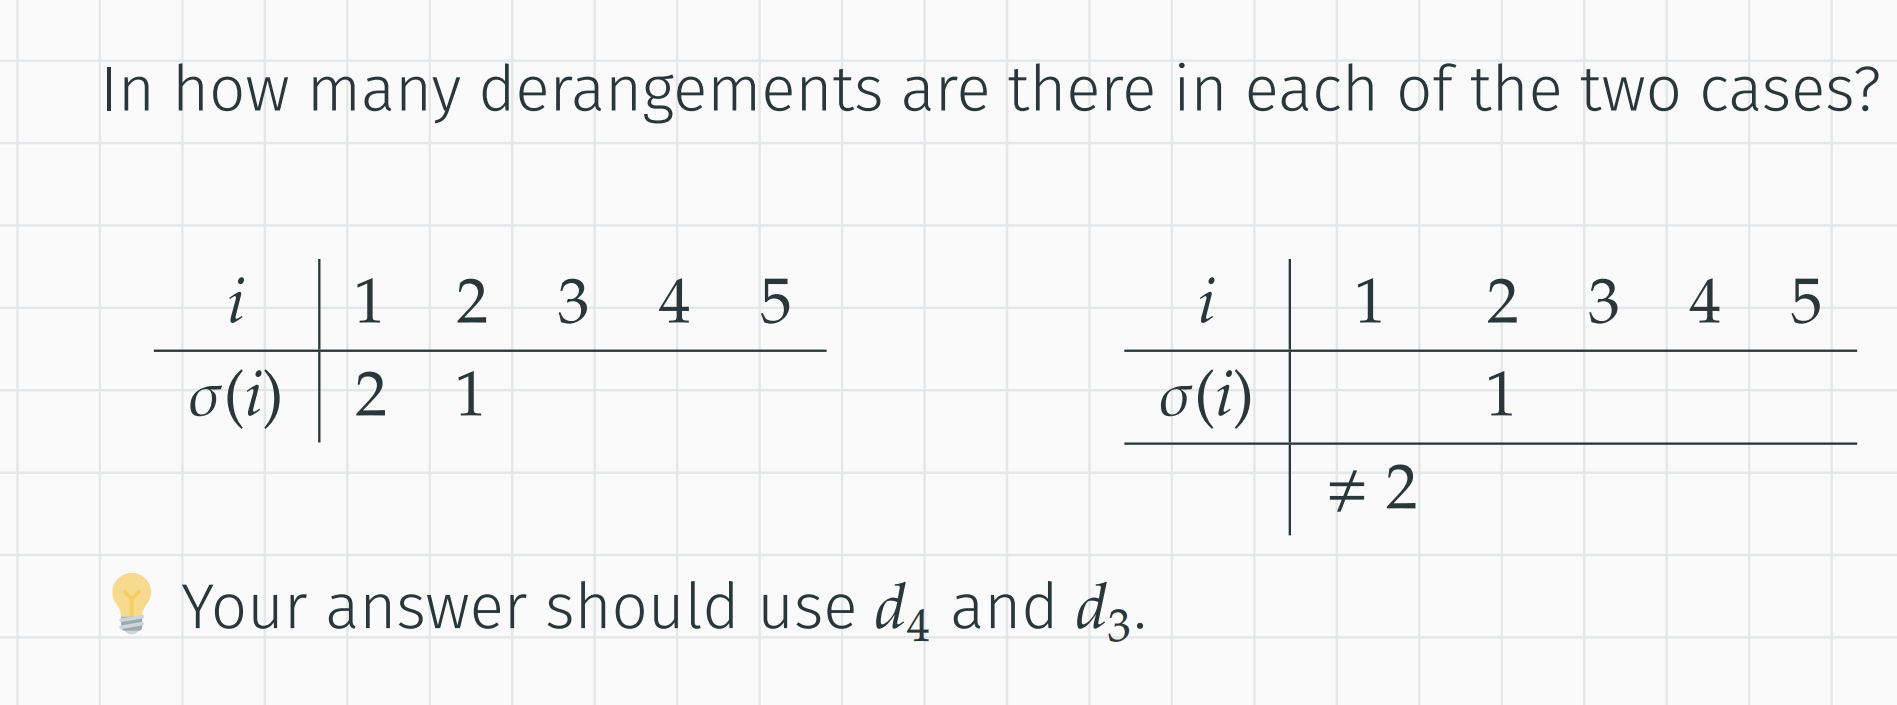
\includegraphics{0006}
For the first, obviously it should be $d_3$\newline
For the second, it should be $d_4$\newline
Explanation:\newline
Solution1:\newline
Simplify the question in to 2 is fixed and position 1 can not have "1" (this is noted as 2) \newline
Thus, it contributes to $d_4$\newline
Solution2:\newline
1) Pretend position 2 fixed, such that we have $d_4$\newline
2) Since position 1 should not be 2, so need to minus the situation that position is 2, which is $d_3$
3) Then we have to put the position 2 back, when position is 1, we have $d_3$ for the rest positions.\newline
4) Therefore, we have $d_4-d_3+d_3=d_4$\newline
\paragraph{A recursive formula of derangement}
We know that $d_1=0$ and $d_2=1$\newline
Give a combinatorial argument that
$$d_n=(n-1)(d_{n-1}+d_{n-2}), for \ n\ge 3$$
For a derangement $\sigma$  consider the integer k with $\sigma (k)=1$\newline
Argue based on the number of choices for k and then two different cases.\newline
$$\sigma (k)=1$$
$$\sigma (k)\neq 1$$
How many derangements are there in each case?
\paragraph{The Euler $\phi$/totient function}
For a positive integer $n \ge 2$, let
$$\phi (n)=|\{m\in [n]:gcd(m,n)=1\}|$$
1) What is $\phi (5)$ and $\phi (9)$\newline
$$\phi (5)=4, \phi(9)=6$$\newline
2) What is $\phi (p)$ when p is prime?\newline
$$\phi(p)=p-1$$\newline
Count multipliers:\newline
Let $n\ge 2,k\ge 1$, and let $p_1,p_2,\cdots p_k$ be distinct primes each of which divide n evenly.\newline
Then the number of integers in [n] which are divisible by each of these k primes is
$$\frac{n}{p_1 p_2 \cdots p_k}$$
Also to an example to compute $\phi (30)$ is 
$$\phi (30)=N(\emptyset)-N(\{1\})-N(\{2\})-N(\{3\})+N(\{1,2\})+N(\{1,3\})+N(\{2,3\})-N(\{1,2,3\})$$
$\Longrightarrow$
$$30-15-10-6+5+2+3-1=8$$
This contributes to a theorem.\newline
Let $n\ge 2$ be a positive integer and suppose that n has m distinct prime factors: $p_1,p_2,\cdots,p_m$. Then
$$\phi (m)=n\prod_{i=1}^m\frac{p_i-1}{p_i}$$
e.g. If $n=7290=2\times 5\times 3^6$, what is $\phi (n)$
$$\phi(7290)=7290\times \frac{1}{2} \times \frac{2}{3} \times \frac{4}{5}=1944$$
\subsubsection{Exercises}
\paragraph{7.7.19}
How many derangements of a nine-element set are there?\newline
Solution:\newline
$$d_9=\sum_{n=0}^9\binom{9}{k}(9-k)!=133496$$
\paragraph{7.7.21}
A careless payroll clerk is placing employees’ paychecks into envelopes that have
been pre-labeled. The envelopes are sealed before the clerk realizes he didn’t match
the names on the paychecks with the names on the envelopes. If there are seven employees, in how many ways could he have placed the paychecks into the envelopes so
that exactly three employees receive the correct paycheck?\newline
Solution:\newline
$$\binom{7}{3}\cdot 4$$
 Label each employee with an element in [7]. There are $\binom{7}{3}$
ways to choose which
employees receive the correct checks. There are $d_4$ ways to arrange the remaining 4 checks so
that no other employee receives their correct check.
\paragraph{7.7.23}
Determine $\phi(18)$ by listing the integers it counts as well as by using the formula of Theorem 7.14.\newline
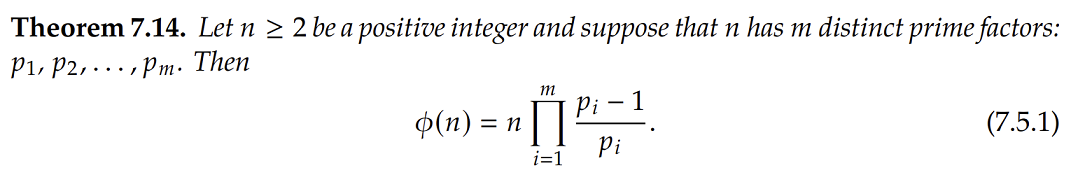
\includegraphics{0012}\newline
Solution:\newline
$$18=2\times 3^2$$
Therefore,
$$\phi (18)=18\cdot \frac{1}{2} \cdot \frac{2}{3}=6$$
\paragraph{7.7.25}Given that
$$1625190883965792=2^5\cdot 3^4\cdot 11^2\cdot 13\cdot 23^3\cdot 181^2$$ compute $\phi(1625190883965792)$\newline
Solution:\newline
$$\phi(1625190883965792)=1625190883965792\times (\frac{1}{2} \cdot \frac{2}{3} \cdot \frac{10}{11} \cdot \frac{12}{13} \cdot \frac{22}{23} \cdot \frac{180}{181})= 4324312852992$$
\paragraph{7.7.27}
At a very small school, there is a class with nine students in it. The students, whom
we will denote as $A, B, C, D, E, F, G, H,$ and $I$, walk from their classroom to the
lunchroom in the order $ABCDEFGHI$. (Let’s say that A is at the front of the line.) On
the way back to their classroom after lunch, they would like to walk in an order so
that no student walks immediately behind the same classmate he or she was behind
on the way to lunch. (For instance, $ACBDIHGFE$ and $IHGFEDCBA$ would meet their
criteria. However, they would not be happy with $CEFGBADHI$ since it contains $FG$
and $HI$, so $G$ is following $F$ again and $I$ is following $H$ again.)\newline
(a) One student ponders how many possible ways there would be for them to line
up meeting this criterion. Help him out by determining the exact value of this
number.\newline
(b) Is this number bigger than, smaller than, or equal to the number of ways they
could return so that no student walks in the same position as before (i.e., A is not
first, B is not second, …, and I is not last)?\newline
(c) What fraction (give it as a decimal) of the total number of ways they could line up
meet their criterion of no student following immediately behind the same student
on the return trip?\newline
Solution:\newline
Let's first try solving a reduced version of this problem. It's always a good idea to solve reduce a problem to a simpler one when you're stuck. Suppose that there are only four students: A, B, C, and D.\newline
\begin{lstlisting}
We can use the Principle of Inclusion-Exclusion to solve this problem. 
1. Case with at least 3 pairs staying the same: ABCD
2. Cases with at least 2 pairs staying the same:
2.1 AB & BC: ABCD, DABC
2.2 AB & CD: ABCD, CDAB
2.3 BC & CD: ABCD, BCDA
3. Cases with at least 1 pair staying the same:
3.1 AB: ABCD, CABD, CDAB, ABDC, DABC, DCAB
3.2 BC: BCAD, ABCD, ADBC, BCDA, DBCA, DABC
3.3 CD: CDAB, ACDB, ABCD, CDBA, BCDA, BACD
4. Cases with at least 0 pairs staying the same:
4!=24 cases.
\end{lstlisting}
So the answer is 24-6-6-6+2+2+2-1=11. \newline
Pattern here:\newline
Do you see a pattern here?

The number of sub-case types: 1, 3, 3, 1.

The number of sub-cases in each type: 1, 2, 6, 24.

Conjecture: For the Lunch Line Problem (yeah I made up that name) with n students, the number of sub-case types within the case with at least k pairs staying the same is $\binom{n-1}{k}$ The number of sub-cases in each type is $(n-k)!$ Therefore the total number of sub-cases where there are at least k pairs staying the same is $$\binom{n-1}{k}(n-k)!=\frac{(n-1)!(n-k)}{k!}$$
Let's prove it. 
\newline
Consider this: if we suppose that two people are together, we can consider them as one person. As an intuitive metaphor, consider them being linked together, forming one "fat man" which can be treated as a whole.
\newline
Therefore, the supposition that one pair stays the same is equivalent to reducing the number of total students by 1. For example, if we know that AB stays the same, this is equivalent to treating AB as a student E and forming the permutations:\newline
$$CDE, CED, DCE, DEC, ECD, EDC$$
Which is exactly the same as the 3-people problem.\newline
Therefore the number of sub-cases is $(n-k)!$ according to the permutations formula.\newline
Regarding the number of sub-case types, there were $n-1$ pairs of students originally. Therefore the number of ways of choosing k pairs should be $\binom{n-1}{k}$\newline
Q.E.D.\newline
With the conjecture proven, the rest is simple. We apply the Principle of Inclusion-Exclusion to get the answer:$$(n-1)!\sum_{k=0}^{n-1}(-1)^k\frac{n-k}{k!}$$
Now plug in $n=9$, the answer is
$$8!\sum_{k=0}^{8}(-1)^k\frac{9-k}{k!}=148329$$
\subsection{Lecture 11}
\subsubsection{Course material}
\paragraph{generating function}
Given an infinite sequence $(a_n)_{n\ge 0}=(a_0,a_1 \cdots)$, we can associate it with a “function”$$
F(x)=\sum_{n\ge 0}a_n X^n$$
called the generating function of $(a_n)_{n\ge 0}$
Be aware that A GF F(x) is not actually a function.\newline
Examples:\newline
What is the GF of $a_0 = 1$, $a_1 = -1$, and $a_n = 0$ for $n\ge 2?$
$$\sum_{n\ge 0}a_n X^n =a_0 X^0+a_1 X^1+\cdots=1-x$$
What is the GF of $a_n = 1$ for $n\ge 0?$
$$\sum_{n\ge 0}a_n X^n =x^0+x^1+\cdots=1+x+x^2+x^3+\cdots =F(x)$$
What is the GF of $a_n = 2^n$ for $n\ge 0?$
$$\sum_{n\ge 0}a_nx^n=2^0\cdot x^0 +2^1\cdot x^1 +\cdots =1+(2x)+(2x)^2+\cdots =F(2x)$$
\paragraph{Multiply GFS}
Multiply polynomials:\newline
$$(1-x)(1+x)=0x^0+(1-1)x^1 (-1)x^2+0x^3=1-x^2$$
Pretend GFS are polynomials:\newline
How should we define the X of GFS such as:
$$(1-x)(1+x+x^2+\cdots)=1-0*x^1+\cdots =1$$
Therefore:\newline
Given two GFS:
$$A(x)=\sum_{n=0}^{\infty}a_n x^n,B(x)=\sum_{n=0}^{\infty}b_n x^n$$,
we define:
$$A(x)B(x)=\sum_{n=0}^{\infty}(\sum_{k=0}^{n}a_kb_{n-k})x^n$$
Multiplicative inverse:\newline
Given $F(x)$, if there exists $G(x)$ such that $G(x)F(x) = 1$, then we
define the multiplicative inverse of $F(x)$ by
$$\frac{1}{F(x)}$$
what is 
$$\frac{1}{1-x}$$
Solution:\newline
Consider that:
$$(1-x)(1+x+x^2+\cdots)=1$$
$\Longrightarrow$
$$\frac{1}{1-x}=(1+x+x^2+\cdots)=\sum_{x=0}^{\infty}x^n$$
Therefore:\newline
Given two GFS:
$$A(x)=\sum_{n=0}^{\infty}a_n x^n,B(x)=\sum_{n=0}^{\infty}b_n x^n$$,
we define:
$$A(x)+B(x)=\sum_{n=0}^{\infty}(\sum_{k=0}^{n}a_n+b_n)x^n$$
More operations of GF:\newline
The derivative $A(x)=\sum_{n=0}^{\infty}a_nx^n$ is defined by
$$\frac{d}{dx}A(x)=\frac{d}{dx}\sum_{n=0}^{\infty}(a_nx^n)=\sum_{n=0}^{\infty}na_nx^{n-1}$$
The integral of $A(x)=\sum_{n=0}^{\infty}a_nx^n$ is defined by
$$\int A(x)dx=\int \sum_{n=0}^{\infty}(a_nx^n)=\sum_{n=0}^{\infty}\frac{1}{n+1}a_nx^{n+1}$$
We also define
$$A(B(x))=\sum_{n=0}^{\infty}a_n{B(x)}^n$$
Shorthand for GFS:\newline
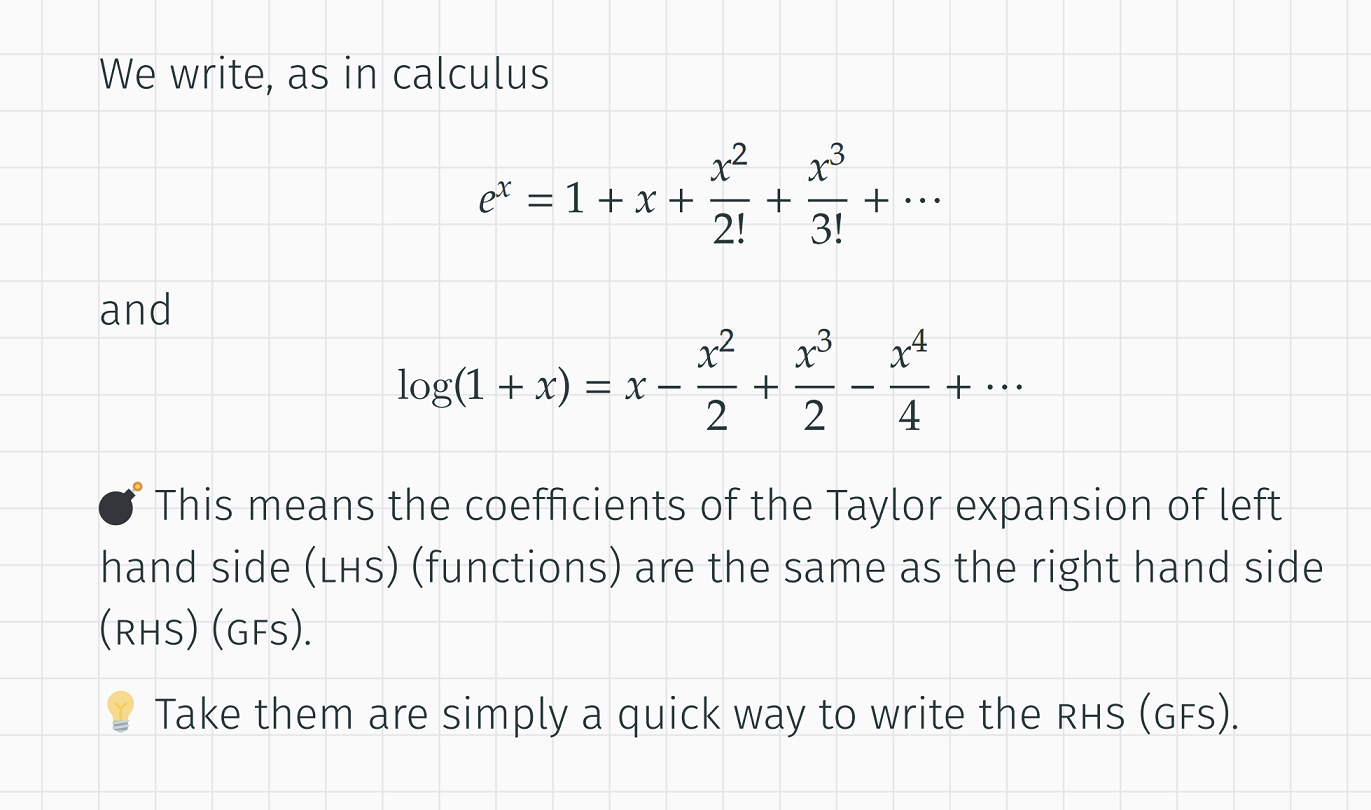
\includegraphics{0007}\newline
Note that as functions:
$$\frac{d}{dx}e^x=e^x$$
and as GFS, we have 
$$\frac{d}{dx}e^x=\frac{d}{dx}\sum_{n=0}^{\infty}\frac{x^n}{n!}=\sum_{n=0}^{\infty}\frac{d}{dx} \frac{x^n}{n!}$$
$\Longrightarrow$
$$\sum_{n=0}^{\infty}\frac{n\cdot x^{n-1}}{n!}=0+\sum_{n=1}^{\infty}\frac{n\cdot x^{n-1}}{n!}$$
$\Longrightarrow$
$$\sum_{n=1}^{\infty}\frac{x^{n-1}}{(n-1)!}=\sum_{n=0}^{\infty}\frac{x^n}{n!}=e^x$$
$$$$
The transfer principle:\newline
If $F(x)=G(x)$ as functions, then F(x)=G(x) as GFS.
\paragraph{TPS-GFS}:\newline
$$(1-x)^n \frac{d^n}{dx^n}\frac{1}{1-x}=n!$$
$$\frac{1}{n!}\frac{d^n}{dx^n}\frac{1}{1-x}=\frac{1}{(1-x)^{n+1}}$$
\paragraph{Different view look at distributions}
n coin, 5 people, everybody at least 1 coin, how many ways \newline
Solution:\newline
$$\binom{n-1}{5-1}$$
Solution with GF:\newline
1) Just one child:\newline
Let $a_n$ be the number of ways to distribute n coins among one
child so that the child has $>$ 0 coin.\newline
Thus,
$$a_n=\begin{cases}0&\text{n=0},\\1&\text{n=1}\end{cases}$$
The GF of $(a_n)_{n\ge 0}$ is 
$$A(x)=\sum_{n\ge 0}a_nx^n=0\cdot x^0+1\cdot x^1+1\cdot x^2+\cdots$$
$\Longrightarrow$
$$=x+x^2+x^3=x\cdot (1+x+x^2+\cdots)$$
$\Longrightarrow$
$$x\cdot \frac{1}{1-x}=\frac{x}{1-x}$$
When there are five children:
Let $b_n$ be the number of ways to distribute n coins among five children so that each child has at least one coin.\newline
We know that
$$b_n=\begin{cases}
0&\text{$n\leq 5$},\\{\binom{n-1}{4}}&\text{$n\ge 5$}\end{cases}$$
So the GF for $(b_n)_{n\ge 0}$ is 
$$B(x) \sum_{n=0}^{\infty}=\sum_{n=5}^{\infty}\binom{n-1}{4}\cdot x^n$$
We notice that
$$A(x)^5=\frac{x^5}{(1-x)^5}=\sum_{n=0}\binom{n-1}{4}x^n=B(x)$$
Proof:
$$\frac{x^5}{(1-x)^5}=\frac{x^5}{4!}\cdot \frac{d^4}{dx^4}\cdot (\frac{1}{1-x})=\frac{x^5}{4!}\cdot \frac{d^4}{dx^4}\cdot x^n$$
$\Longrightarrow$
$$\frac{x^5}{4!}\sum_{n=0}^{\infty}n(n-1)(n-2)(n-3)x^{n-4}$$
$\Longrightarrow$
$$\sum_{n=0}^{\infty}\frac{n(n-1)(n-2)(n-3)}{4!}x^{n+1}=\sum_{n=0}^{\infty}\binom{n}{4}x^{n+1}$$
\subsubsection{Exercises}
\paragraph{8.8.1}
For each finite sequence below, give its generating function.\newline
(a) 1, 4, 6, 4, 1\newline
(b) 1, 1, 1, 1, 1, 0, 0, 1\newline
(c) 0, 0, 0, 1, 2, 3, 4, 5\newline
(d) 1, 1, 1, 1, 1, 1, 1\newline
(e) 3, 0, 0, 1, -4, 7\newline
(f) 0, 0, 0, 0, 1, 2, -3, 0, 1\newline
Solution:\newline
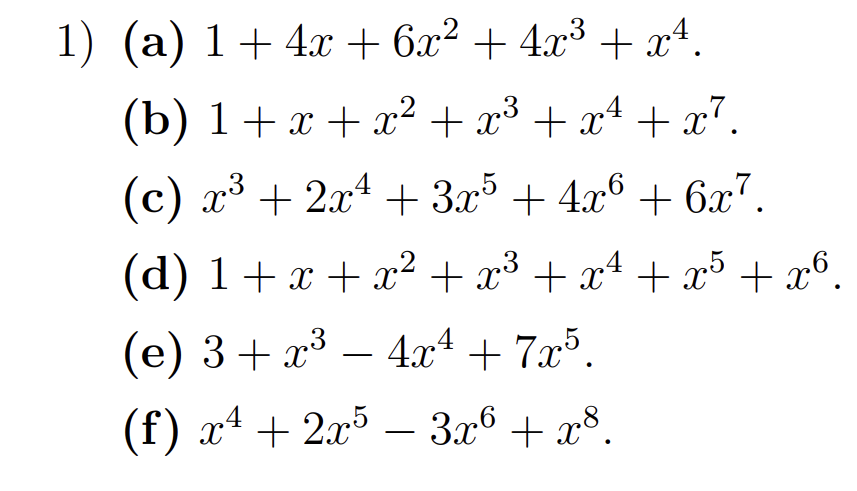
\includegraphics{0013}
\paragraph{8.8.2}
For each infinite sequence suggested below, give its generating function in closed
form, i.e., not as an infinite sum. (Use the most obvious choice of form for the general
term of each sequence.)
\newline
a) 0, 1, 1, 1, 1, 1, $\cdots$\newline
(b) 1, 0, 0, 1, 0, 0, 1, 0, 0, 1, 0, 0, 1, $\cdots$\newline
(c) 1, 2, 4, 8, 16, 32, $\cdots$\newline
(d) 0, 0, 0, 0, 1, 1, 1, 1, 1, 1, 1, 1, 1, 1, 1, $\cdots$\newline
(e) 1, -1, 1, -1, 1, -1, 1, -1, 1, -1, $\cdots$\newline
(f) $2^8$, $2^7\binom{8}{1}$, $2^6\binom{8}{2}$,$\cdots$,$\binom{8}{8}$,0,0\newline
(g) 1, 1, 1, 0, 0, 1, 1, 1, 1, 1, 1, 1, 1, 1, $\cdots$\newline
(h) 0, 0, 0, 1, 2, 3, 4, 5, 6, $\cdots$\newline
(i) 3, 2, 4, 1, 1, 1, 1, 1, 1, $\cdots$\newline
(j) 0, 2, 0, 0, 2, 0, 0, 2, 0, 0, 2, 0, 0, 2, $\cdots$\newline
(k) 6, 0, -6, 0, 6, 0, -6, 0, 6, $\cdots$\newline
(l) 1, 3, 6, 10, 15, $\cdots, \binom{n+2}{2},\cdots$\newline
Solution:\newline
(a)$$\sum_{x=1}^{\infty}=\sum_{x=0}^{\infty}-1=\frac{1}{1-x}-1=\frac{x}{1-x}=-\frac{x}{x-1}$$
(b)$$
\sum_{n=0}^{\infty}x^3=\frac{1}{1-x^3}$$
(c)$$
\sum_{n=0}^{\infty}2^nx^n=\sum_{n=0}^{\infty}(2x)^n=\frac{1}{1-2x}$$
(d)$$\sum_{n=4}^{\infty}x^n=-\frac{x^4}{x-1}$$
(e)$$
\sum_{n=0}^{\infty}(-1)^nx^n=\frac{1}{x+1}$$
(f)$$
\sum_{n=0}^{\infty}2^{8-n}\binom{8}{n}x^n=(x+2)^8$$
(g)$$
\sum_{n=0}^{\infty}x^n-x^4-x^3=-x^4-x^3+\frac{1}{1-x}$$
(h)$$\sum_{n=3}^{\infty}(n-2)x^n=\frac{x^3}{(x-1)^2}$$
(i)$$
\sum_{n=3}^{\infty}x^n+4n^2+2x+3=-\frac{x^3}{x-1}+4x^2=2x+3$$
(j)$$
\sum_{n=0}^{\infty}2x^{3n+1}=\frac{2x}{1-x^3}$$
(k)$$
\sum_{n=0}^{\infty}6x^{4n}+\sum_{n=0}^{\infty}-6x^{4n+2}=\frac{6}{1-x^{4n}}-\frac{6x^2}{1-x^4}$$
(l)$$
\sum_{n=0}^{\infty}\frac{1}{2}(n+1)(n+2)x^n=-\frac{1}{(x-1)^3}$$
\paragraph{8.8.3}
For each generating function below, give a closed form for the $n^th$ term of its associated sequence.\newline
(a)$$(1+x)^{10}$$
(b)$$\frac{1}{1-x^4}$$
(c)$$\frac{x^3}{1-x^4}$$
(d)$$\frac{1-x^4}{1-x}$$
(e)$$\frac{1+x^2-x^4}{1-x}$$
(f)$$\frac{1}{1-4x}$$
(g)$$\frac{1}{1+4x}$$
(h)$$\frac{x^5}{(1-x)^5}$$
(i)$$\frac{x^2+x+1}{1-x^7}$$
(j)$$3x^4+7x^3-x^2+10+\frac{1}{1-x^3}$$
Solution:\newline
(a) By the Binomial Theorem, for $$0\leq n\leq 11, a_n=\binom{10}{11},if \ n\ge 11, a_n=0$$
(b) We have$$\sum_{m=0}^{\infty}x^{4m}=\frac{1}{1-x^4}$$
(c) For $n=4k+3,k\ge 0, c_n=1$, otherwise, $c_n=0$  The generating function looks like
$$x^3(1+x^2+\cdots)=x^3+x^6+\cdots$$
(d)$$\frac{1-x^4}{1-x}=\frac{1}{1-x}-\frac{x^4}{1-x}=\sum_{x^n}^{\infty}-x^4\sum_{n=0}^{\infty}=1+x+x^2+x^3$$
(e) $e_n=1$ for $n\ge 0$ 0 except for n = 3, 4; $e_3 = e_4$ = 2. We combine the following three generating function
$$\frac{1}{1-x}=\sum_{k=0}^{\infty}x^k$$
$$\frac{x^2}{1-x}=\sum_{k=2}^{\infty}x^k$$
$$\frac{x^4}{1-x}=\sum_{k=4}^{\infty}x^k$$
to get that
$$\frac{1+x^2-x^4}{1-x}=1+x+2x^2+2x^3+x^4 +\cdots $$
(f)$$\frac{1}{1-4x}=\sum_{k=0}^{\infty}(4x)^n$$
(g)$$\frac{1}{1+4x}=\sum_{k=0}^{\infty}(-4x)^n$$
(i)$$\sum_{n=0}^{\infty}(x^{7k}+x^{7k+1}+x^{7k+2})$$
\paragraph{8.8.4} Find the coefficient on $x^{10}$ in each of the generating function below.\newline
(a)$$(x^3+x^5+x^6)(x^4+x^5+x^7)(1+x^5+x^10+\cdots)$$
(b)$$(1+x^3)(x^3+x^4+x^5+\cdots)(x^4+x^5+x^6+\cdots)$$
(c)$$(1+x)^{12}$$
(d)$$\frac{x^5}{1-3x^5}$$
(e)$$\frac{1}{(1-x)^3}$$
(f)$$\frac{1}{1-5x^4}$$
(g)$$\frac{x}{1-2x^3}$$
(h)$$\frac{1-x^{14}}{1-x}$$
\subsection{Lecture 12}
\subsubsection{Course materials}
\paragraph{Generating function -coin problem}
n coins, 5 people, everyone at least 2 coins.\newline
Solution:\newline
$$\binom{n-5-1}{5-1}=\frac{1}{24}(n^4-30n^3+335n^2-1650n+3024)$$ for $n\ge 10$ and 0 elsewhere.\newline
GF method:\newline
Just one child: \newline
Let $a_n$ be the number of ways to distribute n coins among one child such that the child has $\ge 2$ coins.\newline
Thus,$$a_n=\begin{cases}0&\text{$n=1$},\\1&\text{$n\ge 2$}\end{cases}$$
The GF of $(a_n)_{n\ge 0}$ is $$
A(x)=\sum_{n=0}a_nx^n=a_0x^0+a_1x^1+a_2x^2\cdots$$
$\Longrightarrow$
$$x^2+x^3+x^4+\cdots=x^2(1+x+x^2+\cdots)$$
$\Longrightarrow$
$$x^2\cdot \frac{1}{1-x}=\frac{x^2}{1-x}$$
When there are five children:\newline
Let $b_n$ be the number of ways to distribute n coins among five children so that each child has $\ge 2$ coins.\newline
Let $B(x)=\sum_{n\ge 0}b_nx^n$.\newline
Thus, by the same argument as before (From Lecture 11)
$$B(x)=A(x)^5=(\frac{x^2}{(1-x)})^5=\sum_{n\ge 0}b_nx^n$$
$\Longrightarrow$
$$(\frac{x^2}{(1-x)})^5=\frac{x^{10}}{(1-x)^5}=x^{10}\cdot \frac{1}{4!}\cdot \frac{d^4}{dx^4}(\frac{1}{(1-x)})=x^{10}\cdot \frac{1}{4!}\cdot \frac{d^4}{dx^4}(\sum_{n=0}^{\infty}x^n)$$
$\Longrightarrow$
$$\frac{x^{10}}{4!}\sum_{n=0}^{\infty}\frac{d^4}{dx^4}x^n=\frac{x^{10}}{4!}\sum_{n=0}^{\infty}n(n-1)(n-2)(n-3)\cdot x^{n-4}$$
$\Longrightarrow$
$$\sum_{n=0}^{\infty}\frac{n(n-1)(n-2)(n-3)}{4!}\cdot x^{n+6}=\sum_{n=0}^{\infty}\binom{n}{4}x^{n+6}$$
$\Longrightarrow$
$$\sum_{n=0+6}^{\infty}\binom{(n+6)-6}{4}x^{n+6}=\sum_{n=6}^{\infty}\binom{n-6}{4}x^n=\sum_{n=0}^{\infty}b_nx^n$$
Thus,
$$b_n=\begin{cases}
    0&\text{$n\leq 5$},\\{\binom{n-6}{4}}&\text{$n > 5$}
\end{cases}$$
\paragraph{A way to get coefficient}
Given$$(\frac{x^2}{(1-x)})^5=\sum_{n\ge 0}b_nx^n$$
Solution:\newline
Base on this formula:
$$\frac{1}{n!}\frac{d^n}{dx^n}\frac{1}{1-x}=\frac{1}{(1-x)^{n+1}}$$
Therefore, we have
$$x{^{10}}\cdot \frac{1}{(1-x)^5}=x^{10}\cdot \frac{1}{4!} \cdot \frac{d^4}{dx^4}(\frac{1}{(1-x)}$$
$\Longrightarrow$
$$$$
$$$$
$$\frac{x^{10}}{4!}\sum_{n=0}^{\infty}n(n-1)(n-2)(n-3)\cdot x^{n-4}$$
\paragraph{Example 8.5}A grocery store is preparing holiday fruit baskets for sale.
Each fruit basket will have n pieces of fruit in it, chosen from apple, banana, carrot, dumpling.\newline
How many different ways can such a basket be prepared if\newline
1. There must be at least one apple in a basket.\newline
2. a basket cannot contain more than three bananas.\newline
3. and the number of carrots must be a multiple of four.\newline
To find the solution:\newline
We can change the problem into 
$$$$
GF for apple:\newline
Let $a_n$ be a number of ways to put in n apples in the basket so
that we have at least one apple.\newline
Thus, the GF for $(a_n)_{n\ge 0}$ is:
$$A(x)=x+x^2+\cdots =\frac{x}{1-x}$$
GF for bananas:\newline
Let $b_n$ be a number of ways to put in n bananas in the basket so
that we have at most 3 bananas.\newline
Thus, the GF for $(b_n)_{n\ge 0}$ is:
$$B(x)=x+x^2+x^3$$
GF for carrots:\newline
Let $c_n$ be a number of ways to put in n carrots in the basket so
that we have a multiple of four carrots.\newline
Thus, the GF for $(c_n)_{n\ge 0}$ is:
$$C(x)=1+x^4+x^8+\cdots =\frac{1}{1-x^4}$$
GF for dumpling:\newline
Let $d_n$ be a number of ways to put in n dumplings in the basket.\newline
Thus, the GF for $(d_n)_{n\ge 0}$ is:
$$D(x)=x+x^2+x^3+\cdots =\frac{1}{1-x}$$
Therefore, here comes the GF for four fruit basket.\newline
Let $e_n$ be the number of ways to put n fruits in the basket so all
conditions are satisfied.
The GF for $(e_n)_{n\ge 0}$ is:
$$\sum_{n=0}^{\infty}=A(x)B(x)C(x)D(x)$$
$\Longrightarrow$
$$\frac{x}{1-x}(1+x+x^2+x^3)\frac{1}{1-x^4}\frac{1}{1-x}$$
$\Longrightarrow$
$$\sum_{n=0}\binom{n+1}{2}x^n$$
\paragraph{Newton's Binomial Theorem: Beginning}
$$2^{2n}=\sum_{k=0}^{n}\binom{2k}{k}\binom{2n-2k}{n-k},(n\in N)$$
1)Can we get this with GF?\newline
2)Can you find one combinatorial proof?\newline
proof:\newline
The LHS counts all possible ways of placing 2n pairs of parentheses, regardless of the partition of the 2n elements into groups.
\newline
The RHS counts the number of ways to partition the 2n elements into k groups of consecutive elements, where each group has either 0 or 2 pairs of parentheses. Each group can be counted using a binomial coefficient: $\binom{2k}{k}$ counts the number of ways to choose the k pairs of parentheses within the first k elements, and $\binom{2n-2k}{n-k}$ counts the number of ways to choose the n-k pairs of parentheses within the last n-k elements. The sum of all such partitions over k gives us the total number of ways to place 2n pairs of parentheses.
\newline
Thus, the combinatorial proof is that both the LHS and RHS of the equation are counting the same quantity, and so they must be equal.\newline
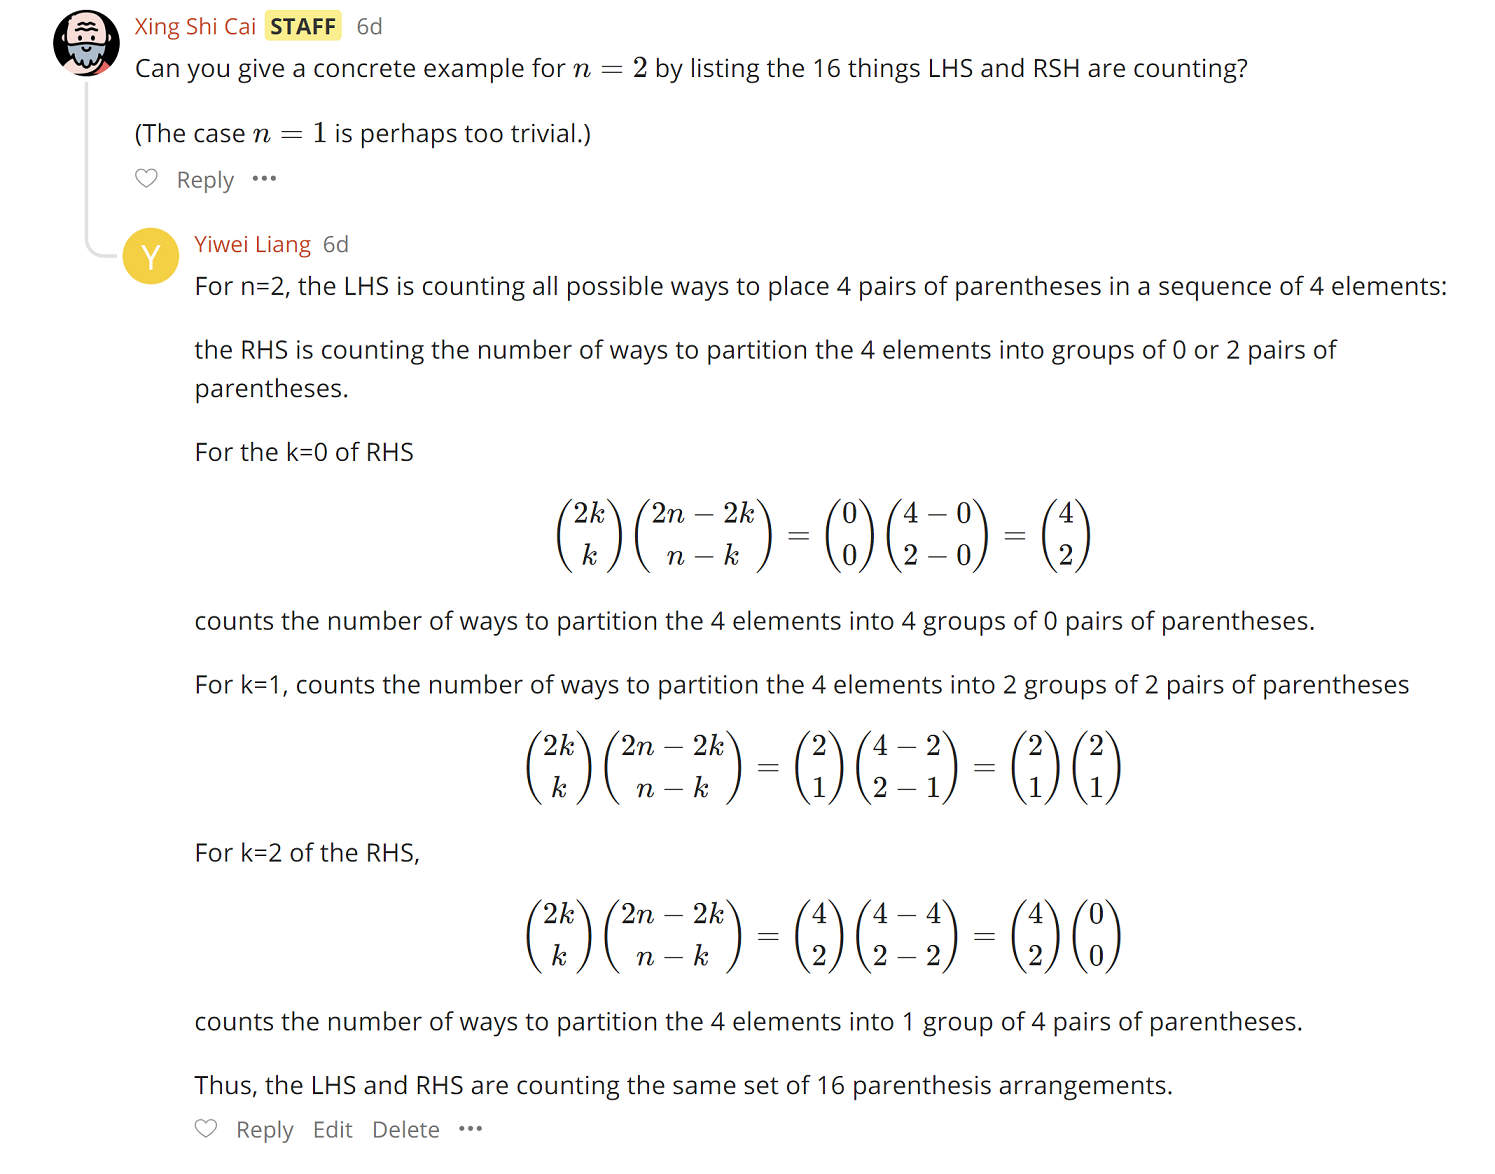
\includegraphics{0023}
\paragraph{Newton's Binomial Theorem: Definition 8.8}
For all $p\in R$ and $k\in N$, the number P(p,k) is defined by\newline
1. P(p,0)=1 for all real number p and,\newline
2. P(p,k)=pP(p-1,k-1) for all real numbers p and integers $k>0$\newline
e.g.\newline
$$P(3,2)=3\cdot P(3-1,2-1)=\cdots=3\cdot 2\cdot 1 =6$$
\paragraph{Newton's Binomial Theorem: Definition 8.9}
For all $p\in R$ and $k\in N$
$$\binom{p}{k}=\frac{P(p,k)}{k!}$$
By Theorem 2.30 (ac): we have \newline
For all $p\in N$ with $p\ge 0$,
$$(1+x)^p=\sum_{n=0}^{p}\binom{p}{n}x^n$$
And here is the Newton-version:
$$(1+x)^p=\sum_{n=0}^{\infty}\binom{p}{n}x^n$$
\paragraph{Applying Newton’s Binomial Theorem} 
Lemma 8.12:\newline
For all integer $k\ge 0$
$$\binom{-\frac{1}{2}}{k}=(-1)^k\frac{\binom{2k}{k}}{2^{2k}}$$
Proof Theorem 8.13(AC)
$$\frac{1}{\sqrt{1-4x}}=\sum_{n\ge 0}\binom{2n}{n}x^n$$
Proof:
$$(1-4x)^{-\frac{1}{2}}=\sum_{n=0}^{\infty}\binom{-\frac{1}{2}}{n}\cdot (-4x)^n=\sum_{n=0}^{\infty}(-1)^n\frac{\binom{2n}{n}}{2^{2n}}\cdot (-4)^n \cdot x^n=\sum_{n=0}^{\infty}\binom{2n}{n}\cdot x^n$$
Corollary 8.14(AC):\newline
For all integer $n\ge 0$
$$4^n=2^{2n}=\sum_{k\ge 0}\binom{2k}{k}\binom{2n-2k}{n-k}=\sum_{k=0}^na_n\cdot a_{n-k}$$
To find a GF:
$$(LHS)^2=(1-4k)^{-1}=\frac{1}{1-4k}=\sum_{n=0}^{\infty}(4^n)x^n$$
$$(RHS)^2=(\sum_{n=0}^{\infty}a_n\cdot x_n)(\sum_{n=0}^{\infty}a_n\cdot x_n)=\sum_{n=0}^{\infty}(\sum_{k=0}^na_n\cdot a_{n-k})x^n$$
\subsubsection{Exercises}
\paragraph{8.8.5}
Find the generating function for the number of ways to create a bunch of n balloons
selected from white, gold, and blue balloons so that the bunch contains at least one
white balloon, at least one gold balloon, and at most two blue balloons. How many
ways are there to create a bunch of 10 balloons subject to these requirements?\newline
Solution:\newline
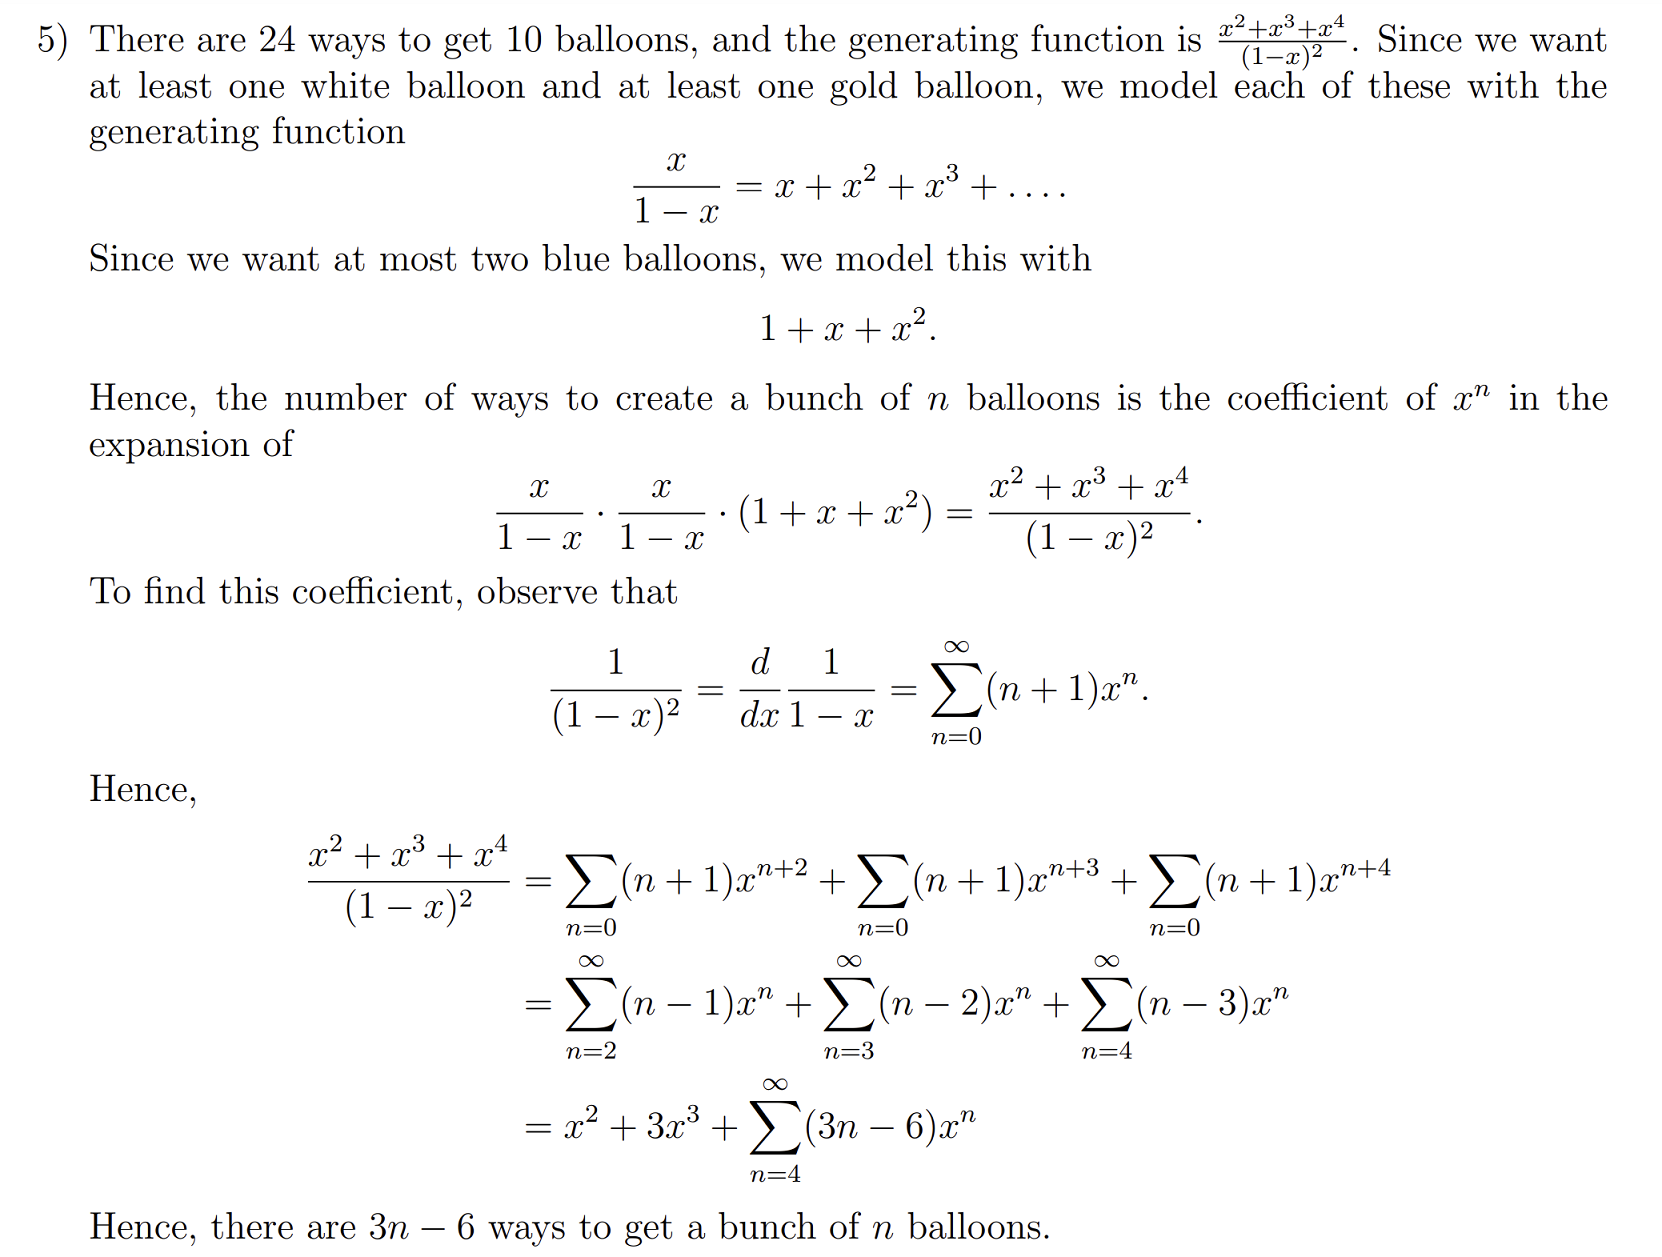
\includegraphics{0015}
\paragraph{8.8.7}
Consider the inequality $$x_1+x_2+x_3+x_4\leq n$$
where $x_1, x_2, x_3, x_4, n$ $\ge$ 0 are all integers. Suppose also that x2 $\ge$ 2, x3 is a multiple of
4, and 0 $\leq$ x4 $\leq$ 3. Let $c_n$ be the number of solutions of the inequality subject to these
restrictions. Find the generating function for the sequence $\{c_n:n\ge 0\}$ and use it to
find a closed formula for $c_n$\newline
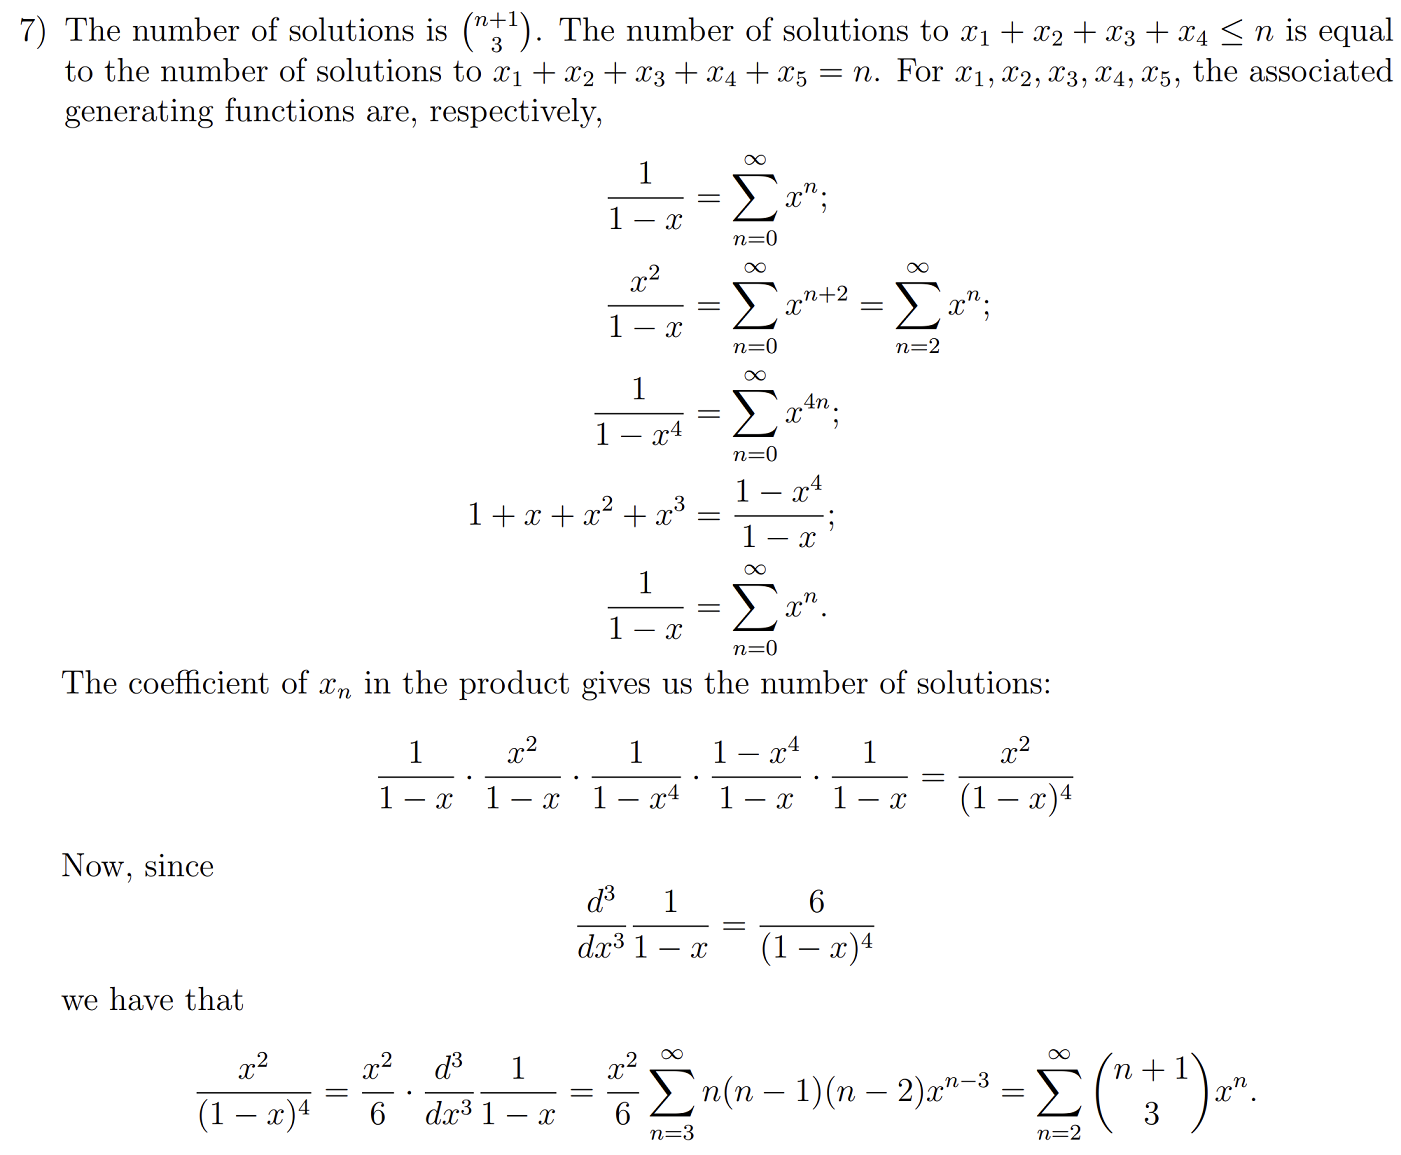
\includegraphics{0016}
\paragraph{8.8.9}
What is the generating function for the number of ways to select a group of n students from a class of p students?\newline
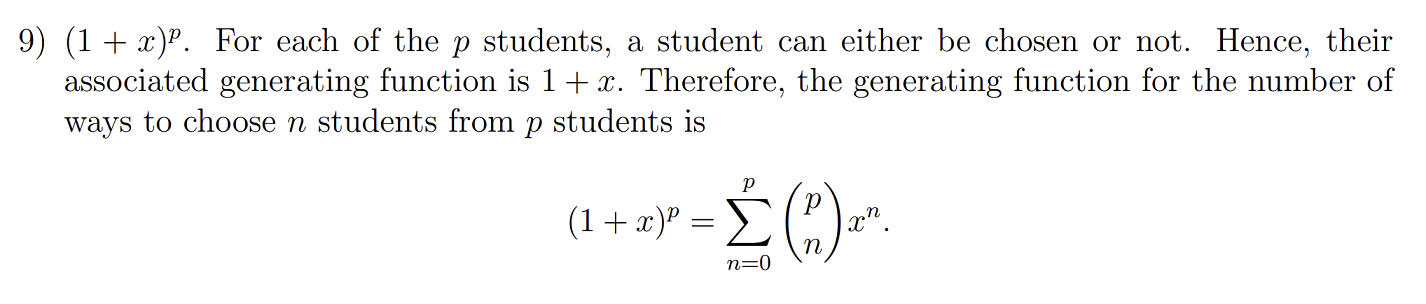
\includegraphics{0017}
\paragraph{8.8.11}
Using generating functions, find the number of ways to make change for a 100
dollar bill using only dollar coins and \$1, \$2, and \$5 bills. \newline
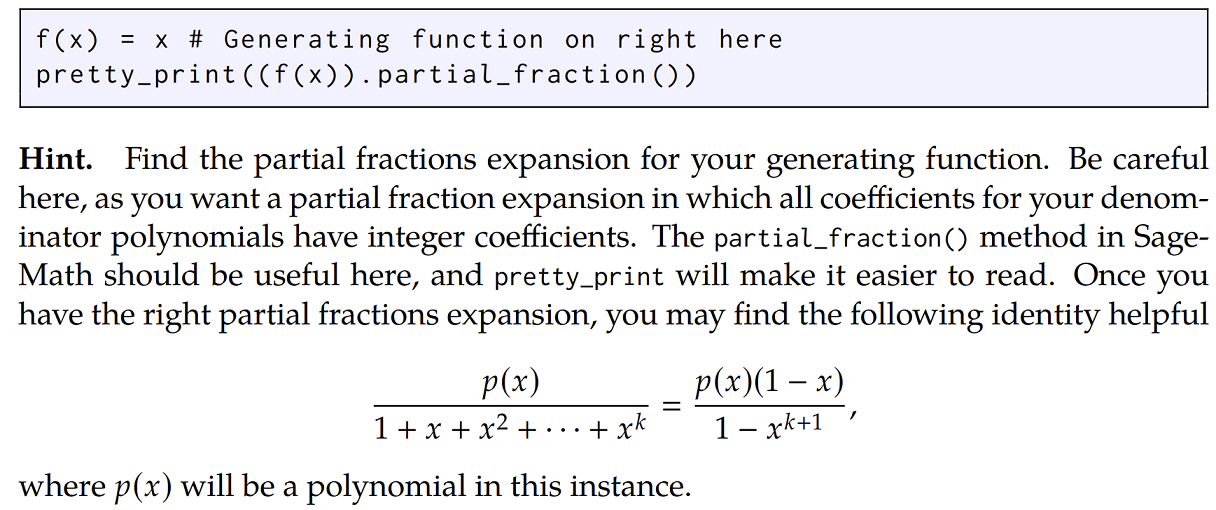
\includegraphics{0014}\newline
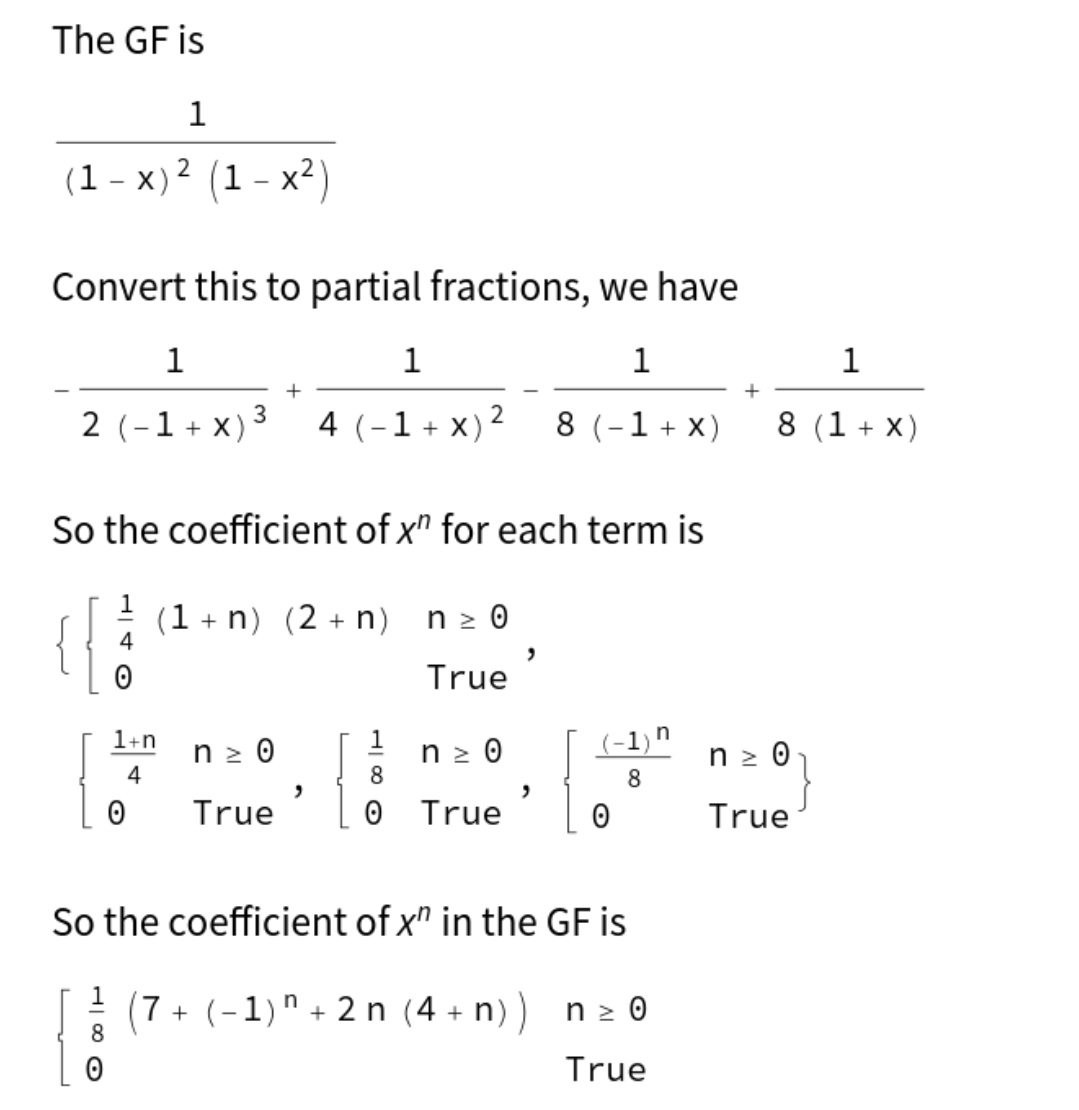
\includegraphics{0018}
\paragraph{8.8.13}
Bags of candy are being prepared to distribute to the children at a school. The
types of candy available are chocolate bites, peanut butter cups, peppermint candies,
and fruit chews. Each bag must contain at least two chocolate bites, an even number of peanut butter cups, and at most six peppermint candies. The fruit chews are available
in four different flavors—lemon, orange, strawberry, and cherry. A bag of candy may
contain at most two fruit chews, which may be of the same or different flavors. Beyond
the number of pieces of each type of candy included, bags of candy are distinguished
by using the flavors of the fruit chews included, not just the number. For example, a
bag containing two orange fruit chews is different from a bag containing a cherry fruit
chew and a strawberry fruit chew, even if the number of pieces of each other type of
candy is the same.\newline
(a) Let $b_n$ be the number of different bags of candy with n pieces of candy that can be
formed subject to these restrictions. Find the generating function for the sequence
${b_n : n \ge 0}$\newline
(b)) Suppose the school has 400 students and the teachers would like to ensure that
each student gets a different bag of candy. However, they know there will be
fights if the bags do not all contain the same number of pieces of candy. What is
the smallest number of pieces of candy they can include in the bags that ensures
each student gets a different bag of candy containing the same number of pieces
of candy?\newline
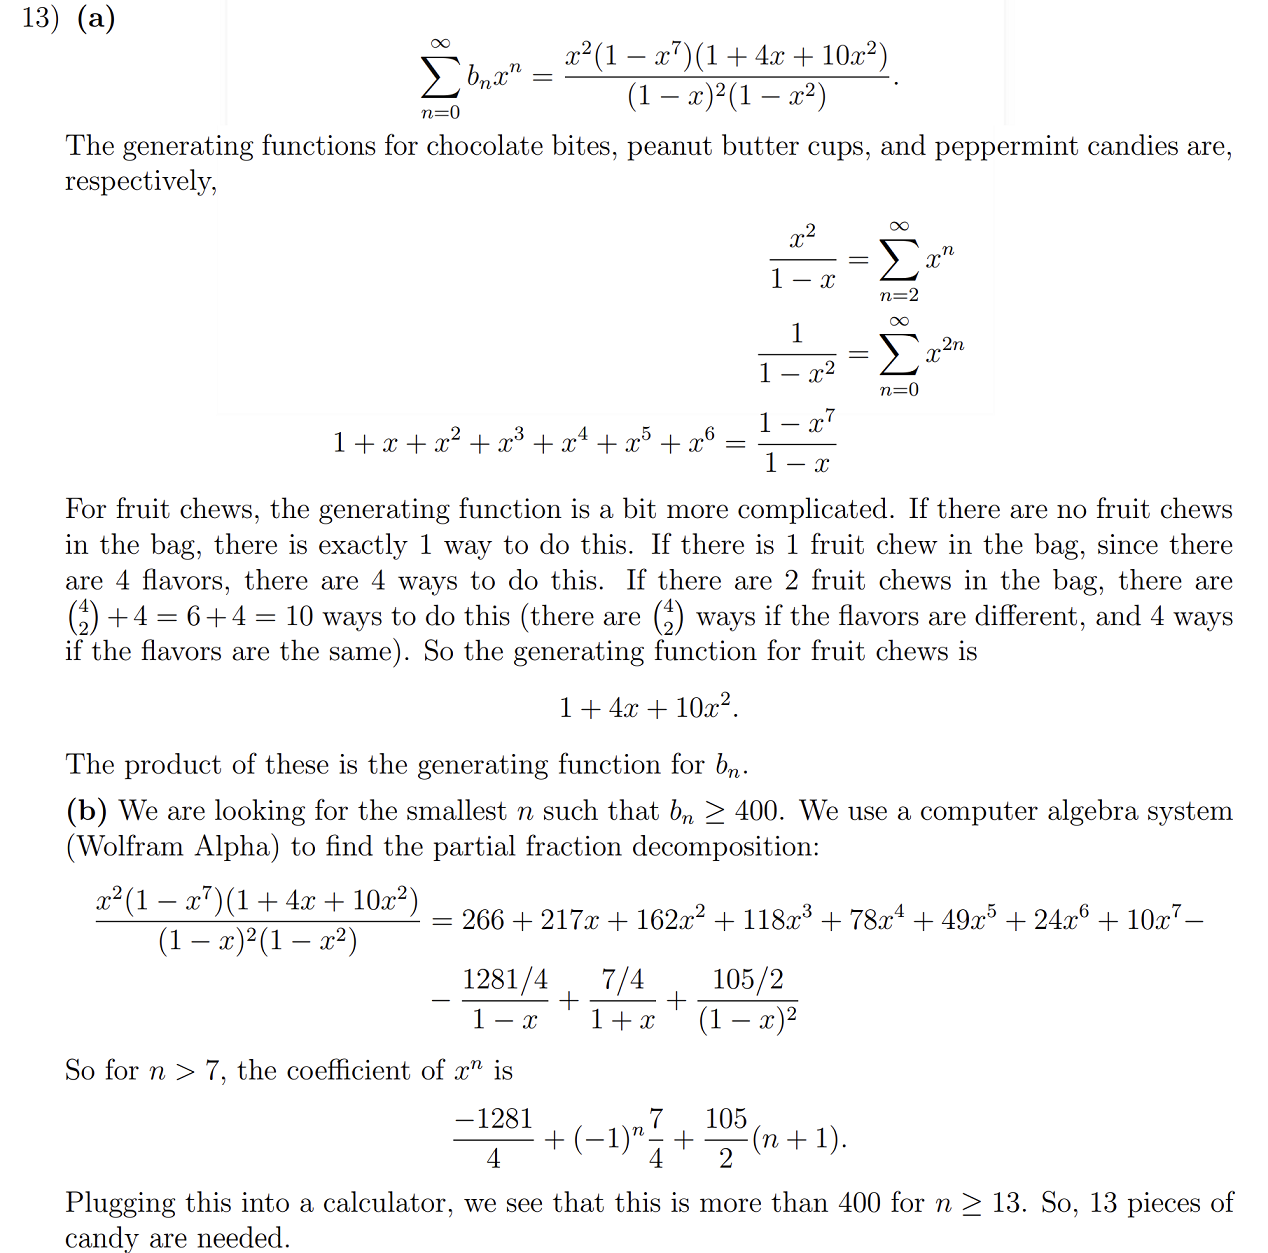
\includegraphics{0019}
\paragraph{8.8.15}Tollbooths in Illinois accept all U.S. coins, including pennies. Carlos has a very
large supply of pennies, nickels, dimes, and quarters in his car as he drives on a tollway. He encounters a toll for \$ 0.95 and wonders how many different ways he could
use his supply of coins to pay the toll without getting change back. (A computer algebra system is probably the best way to get the required coefficient once you have a
generating function, since you’re not asked for the coefficient on $x^n$.)\newline
(a) Use a generating function and computer algebra system to determine the number
of ways Carlos could pay his \$ 0.95 toll by dropping the coins together into the
toll bin. (Assume coins of the same denomination cannot be distinguished from
each other.)\newline
(b) Suppose that instead of having a bin into which motorists drop the coins to pay
their toll, the coins must be inserted one-by-one into a coin slot. In this scenario,
Carlos wonders how many ways he could pay the \$ 0.95 toll when the order the
coins are inserted matters. For instance, in the previous part, the use of three quarters and two dimes would be counted only one time. However, when the coins must be inserted individually into a slot, there are 10  C(5, 2) ways to insert this
combination. Use a generating function and computer algebra system to determine the number of ways that Carlos could pay the \$ 0.95 toll when considering
the order the coins are inserted.\newline
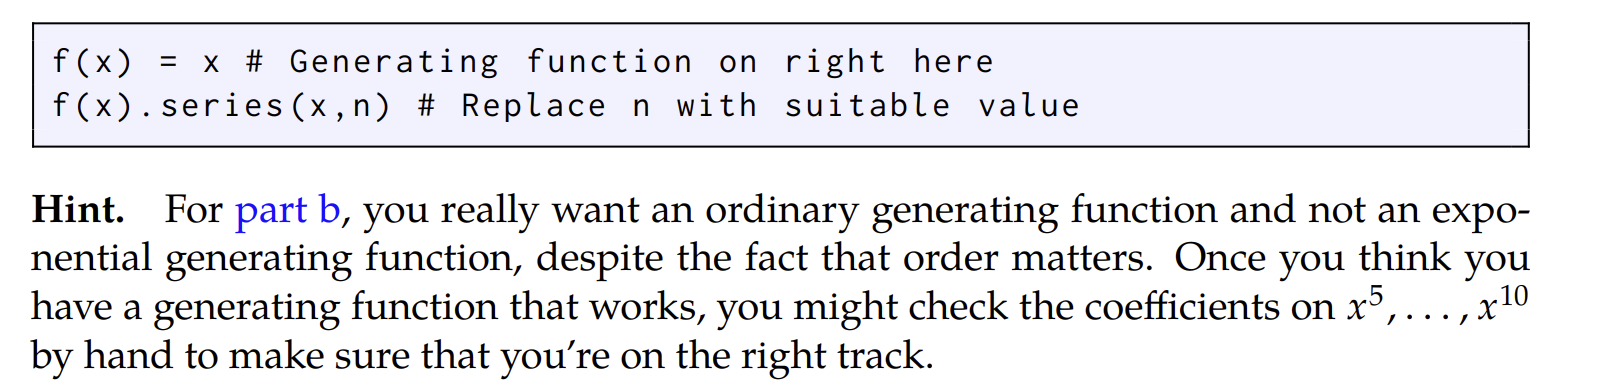
\includegraphics{0020}\newline
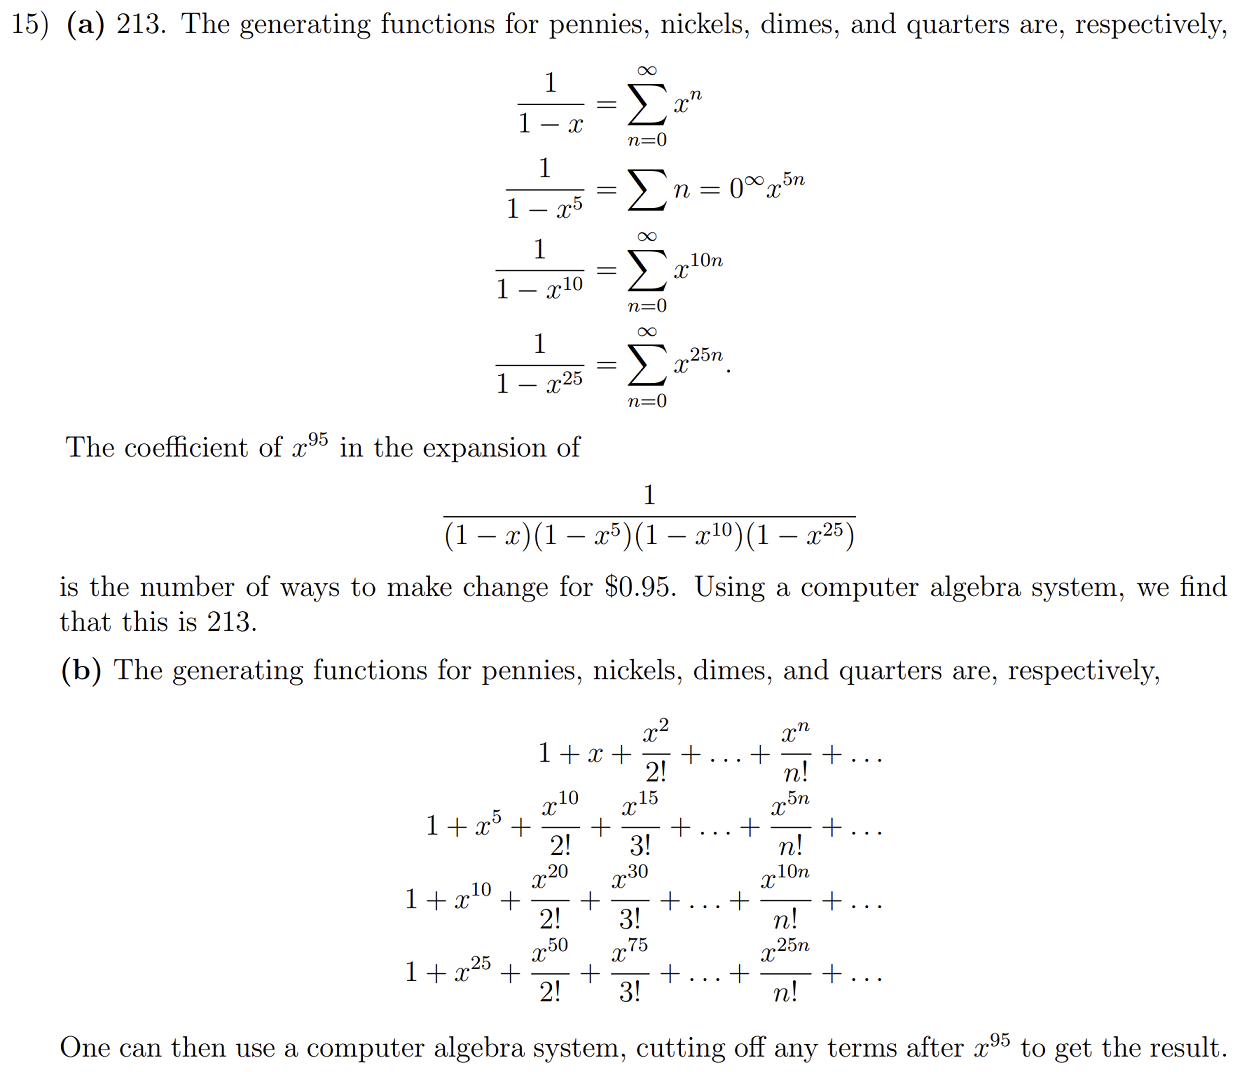
\includegraphics{0021}
\newpage \section{Week4}
\subsection{Lecture 13}
\subsubsection{Course materials}
\paragraph{Paying lunch with cash}
You forgot your phone at home so you have to pay your lunch with
cash.\newline
How many ways can you pay \$100 with \$1, \$2, \$5 bills?\newline
Paying with \$1 bills:\newline
Let $a_{1,n}$ be the number of ways to pay \$n with \$1 bills.\newline
The generating function (GF) $A_1$ of $(a_{1,n})_{n\ge 0}$ is
$$1+x+x^2+\cdots =\frac{1}{1-x}$$
Quick review - How is the = defined here?\newline
$$F(x)\cdot G(x)=1 \Longrightarrow F(x)=\frac{1}{G(x)}$$
Paying with \$2 bills:\newline
Let $a_{2,n}$ be the number of ways to pay \$n with \$1 bills.\newline
The generating function (GF) $A_2$ of $(a_{2,n})_{n\ge 0}$ is
$$1+x^2+x^4+\cdots =\frac{1}{1-x^2}$$
$$b_n=\begin{cases}
    0&\text{n is odd},\\{1}&\text{n is even}
\end{cases}$$
Paying with \$5 bills:\newline
Let $a_{5,n}$ be the number of ways to pay \$n with \$1 bills.\newline
The generating function (GF) $A_5$ of $(a_{5,n})_{n\ge 0}$ is
$$1+x^5+x^{10}+\cdots =\frac{1}{1-x^5}$$
Therefore, let Let $a_n$ be the number of ways to pay \$n with \$1, \$2, \$5 bills.\newline
The GF of $(a_n)_{n\ge 0}$ is
$$A(x)=A_1(x)A_2(x)A_5(x)=\frac{1}{1-x}\frac{1}{1-x^2}\frac{1}{1-x^5}$$
Remind that  There is no closed form for $a_n$.\newline
But it is easy to get that $a_{100}$ is 541.\newline
Paying with \$ m bills:\newline
Let $a_m,n$ be the number of ways to pay \$ n with \$ m bills for some integer m $>$ 0.\newline
The GF $A_m(x)$ of $(a_(m,n))_{n\ge 0}$ is 
$$1+x^m+x^{2m}+\cdots=\frac{1}{1-x^m}$$
Paying lunch with more cash:\newline
the GF will be $$\prod_{m=1}^{\infty}\frac{1}{1-x^m}$$
\paragraph{The integer partition problem}
For $n\in N$, $P_n$
is also the number of integer solutions of
$$a_1+a_2+\cdots+a_k=n$$
for some $k\in N$ such that $a_1\ge a_2\ge \cdots \ge a_k>0$
It has same solution above.
\paragraph{Paying with money of odd values}
Let $o_n$ be the number of ways to pay \$n with \$1, \$3, \$5 …bills.\newline
Then what is the GF of $(o_n)_{n\ge 0}$
$$O(x)=\sum_{n=0}^{\infty}o_nx^n=\prod_{n=0}^{\infty}\frac{1}{1-x^{2n+1}}$$
The first few of $O_n$ are (by OEIS):
$$1, 1, 1, 2, 2, 3, 4, 5, 6, 8, 10, 12, 15$$
\paragraph{Paying with money of distinct values}
Let $d_n$ be the number of ways to pay \$n with \$1, \$3, \$5 …bills.\newline
Then what is the GF of $(d_n)_{n\ge 0}$
$$D(x)=\sum_{n=0}^{\infty}d_nx^n=\prod_{n=0}^{\infty}(1+x^n)$$
The first few of $O_n$ are (by OEIS):
$$1, 1, 1, 2, 2, 3, 4, 5, 6, 8, 10, 12, 15$$

\paragraph{Exponential Generating Function}
Given an infinite sequence $(a_n)_{n\ge 0}=(a_0,a_1,),\cdots$ we associate it
with a “function” F(x) written as $$F(x)=\sum_{n\ge 0}\frac{a_n}{n!}x^n$$
called the exponential generating function (exponential generating function (egf)) of $(a_n)_{n\ge 0}$.\newline
In other words, the EGF of $a_n$ is the GF of $\frac{a_n}{n!}$
\paragraph{Strings consisting of one letters}
Let $a_n$ be the number of strings of length n consisting of only one letter apple.\newline
What is $a_n$?\newline
$a_0=1,a_1=1,a_2=1 \Longrightarrow a_n=1 \ for n\in N$\newline
Let $a_n$ be the number of strings of length n consisting of only one letter.\newline
What is $a_n$?\newline
The exponential generating function of $(a_n)_{n\ge 0}$ is $$A(x)=\sum_{n=0}^{\infty}\frac{a_n}{n!}x^n=1+x+\frac{x^2}{2!}+\cdots +=e^x$$
$\Longrightarrow$
$$=\sum_{n=0}^{\infty}\frac{1}{n!}x^n$$
\paragraph{Strings consisting of two letters}
Let $b_n$ be the number of strings of length n consisting of either letter apple or banana.\newline
What is $b_n$?
$$2^n$$
The exponential generating function of $(b_n)_{n\ge 0}$ is $$B(x)=\sum_{n=0}^{\infty}\frac{b_n}{n!}x^n=1+(2x)+\frac{(2x)^2}{2!}+\frac{(2x)^3}{3!}+\cdots =e^{2x}$$
Note that 
$$A(x)A(x)=e^xe^x=e^{2x}=B(x)$$
There is no coincidence in this class.
\paragraph{Common way to compute EGF}
Let’s compute the coeffcient of, say $x^3$, in the EGF $$A(x)A(x)=(\sum_{n\ge 0}\frac{a_n}{n!}x^n)(\sum_{n\ge 0}\frac{a_n}{n!}x^n)=\cdots+(\sum_{k=0}^3\frac{a_k}{k!}\cdot \frac{a_{n-k}}{(n-k)!}x^3)+\cdots $$
\paragraph{String with even number of carrots}
Let $c_n$ be the number of strings consisting only of even number of carrots.\newline
The exponential generating function of $(c_n)_{n\ge 0}$ is 
$$C(x)=\sum_{n=0}^{\infty}\frac{c_n}{n!}=1+\frac{x^2}{2}+\cdots +\frac{e^x+e^{-x}}{2}$$
\paragraph{Ternary strings with even number of carrots}
Let $d_n$ be the number of ternary strings consisting of apples, bananas and even number of carrots.\newline
The exponential generating function of $(d_n)_{n\ge 0}$ is $$D(x)=C(x)A(x)A(x)=\frac{e^x+e^{-x}}{2}\cdot e^x\cdot e^x$$
So $$d_n=\frac{3^n+1}{2}$$
\subsubsection{Exercises}
\paragraph{8.8.17}
Use generating functions to find the number of ways to partition 10 into odd parts.\newline
Solution:\newline
A partition of 10 into odd parts consists of 1s, 3s, 5s, 7s, and 9s. The generating function for
each of these is, respectively,\newline
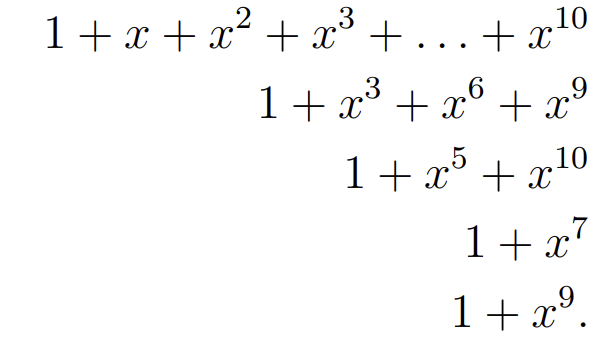
\includegraphics{0042}\newline
Hence, the coefficient of $x^10$ in the product of these gives the answer. Multiplying these
polynomials together with a computer algebra system yields 10 as the coefficient of $x^10$
\paragraph{8.8.19}
What is the generating function for the number of partitions of an integer into even parts?\newline
Solution:\newline
$$\prod_{n=1}^{\infty}\frac{1}{1-x^{2n}}$$
\paragraph{8.8.21}
For each exponential generating function below, give a formula in closed form for the sequence ${a_n:n\ge 0}$ it represents.
$$(a) e^{7x}\ (b)x^2e^{3x}\ (c)\frac{1}{1+x}\ (d)e^{x^4}$$
Solution:\newline
(a) $$a_n=7^n$$ because
$$e^{7x}=1+7x+\frac{(7x)^2}{2!}+\cdots$$
(b) $$a_n=n(n-1)3^{n-2}$$
(c) $$n!(-1)^n$$
(d) Replace $x^4$ by y, we have 
$$e^{x^4}=e^y=\sum_{n=0}^{\infty}\frac{y^n}{k!}=\sum_{n=0}^{\infty}\frac{x^{(4n)}}{n!}$$
\paragraph{8.8.23}Find the exponential generating function for the number of strings of length n
formed from the set $\{a, b, c, d\}$ if there must be at least one a and the number of c’s
must be even. Find a closed formula for the coefficients of this exponential generating
function.\newline
Solution:\newline
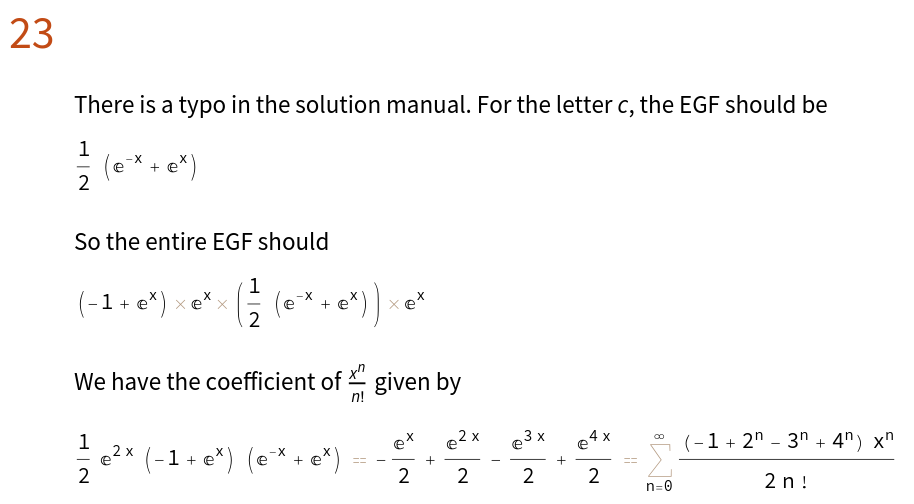
\includegraphics{8.8.23}
\paragraph{8.8.25}
Find the exponential generating function for the number of strings of length n
formed from the set $\{a, b, c, d\}$ if there must be at least one a, the number of b’s must
be odd, and the number of d’s is either 1 or 2. Find a closed formula for the coefficients
of this exponential generating function.\newline
Solution:\newline
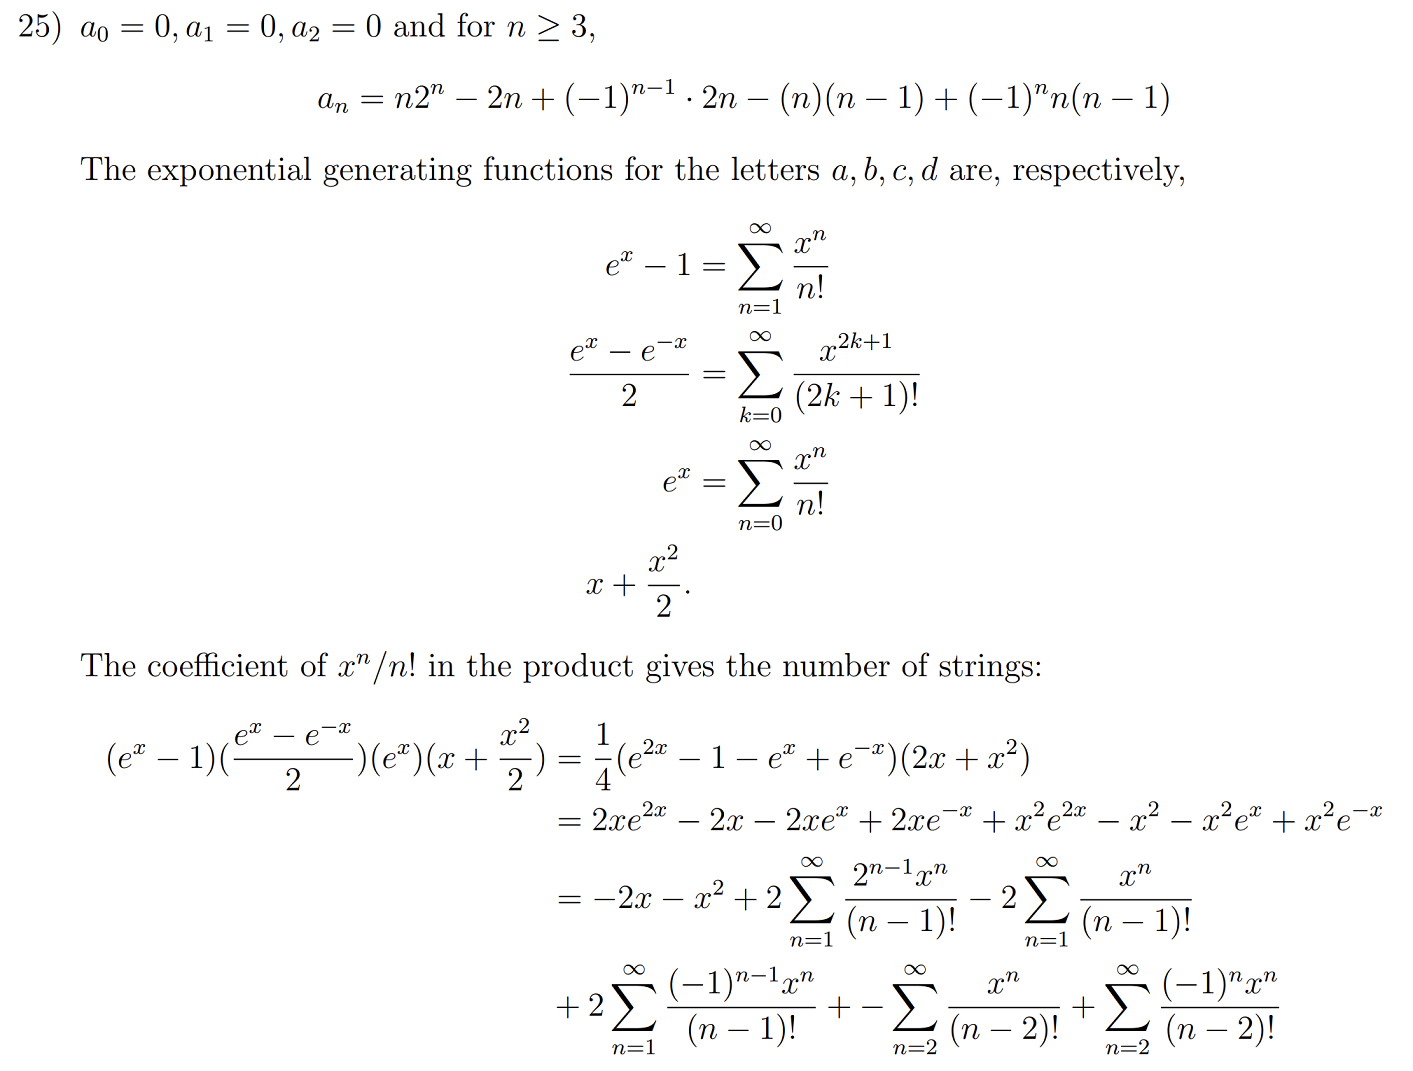
\includegraphics{0044}
\paragraph{8.8.27}
Consider the inequality $$x_1+x_2+x_3+x_4\leq n$$
where $x_1,x_2,x_3,x_4,n\ge 0$ are all integers. Suppose also that $x_2\ge 2$, $x_3$ is multiple of 4, and $1\leq x_4\leq 3$. Let $c_n$ be the number of solutions of the inequality subject to these restrictions. Find the generating function for the sequence $\{c_n: n\ge 0\}$ and use it to find a closed formula for $c_n$. \newline
Hint. Yes, this is very close to Exercise 8.8.7. However, the bounds on $x_4$ are different
here. You might try using a computer algebra system to expedite finding the partial fractions expansion, which will have several terms whose power series you can work with quickly. For the term involving $\frac{1}{(1+x^2)}$, work out the series by hand. You may find that your solution to this problem has two parts—one for when n is even and another for when n is odd.\newline
Solution:\newline

\subsection{Lecture 14}
\subsubsection{Course material}
\paragraph{Closed form vs recurrence}
$$r_n=r{n-1}+n, (n\ge 1)$$
This is called a recurrence equation.
Note that we can also consider the sequence $(r_n)_{n\ge 0}$ as a
function r: $N\longrightarrow N$ and write
$$r(n)=r(n-1)+n, (n\ge 1)$$
Can we find a closed formula for $r_n$?
$$r_n=r_{n-1}+n=r_{n-2}+(n-1)+n=\cdots =r_0+1+2+\cdots =1+\frac{n(n+1)}{2} $$
\paragraph{Linear recurrence equations}
A sequence $(a_n)_{n\ge 0}$ satisfies a linear recurrence if $$c_0a_{n+k}+c_1a_{n+k-1}=\cdots +c_ka_n=g(n)$$
where $k\ge 1$ is an integers, $c_0,c_1,\cdots c_k$ are constants with $c_0,c_k\neq 0$ and g is a function.\newline
The order of the recurrence is k.\newline
Why do we want $c_0,c_k\neq 0$ in the definition?\newline
Because if $c_0=0$, the order will be incorrect. And we want the order k recurrence to have k+1 terms.
\paragraph{Homogeneous and Nonhomogeneous recurrence}
The recursion is homogeneous if $g(n)$ is always 0, like the
Fibonacci sequence -
$$f_{n+2}-f_{n+1}-f(n)=0$$
Otherwise it is nonhomogeneous, like the crown sequence -
$$r_{n+1}-r_n=n+1$$
\paragraph{Advancement operator}
Let $Af(n)=f(n+1)$ and $A^pf(n)=f(n+p)$.
The recursion for Fibonacci sequence
$$f(n+2)-f(n+1)-f(n)=0$$
can be written as 
$$A^2f(n)-Af(n)-A^0f(n)=0$$
We abbreviate this by
$$(A^2-A-1)f=0$$
e.g. $$A^2f=f(n+2)$$
$$A^3=f(n+3)=A(A(A(f)))$$
\paragraph{Polynomials of advancement operator}
If $p(A)=q(A)$ holds as polynomials of the variable A, then
$p(A)f=q(A)f$ as functions.\newline
Example: Since $$(A-2)(A+3)=A^2+A-6$$.
We have $$(A-2)(A+3)f=(A^2+A-6)f$$
Can you check this?
$$RHS: (A^2+A-6)f=A^2+Af-6A^0=f(n+2)+f(n+1)-6f(n)$$
$$LHS:(A+3)f=(A+3A^0)f=Af+3A^0f=f(n+1)+3f(n)$$
$$(A-2)[f(n+1)+3f(n)]=A(f(n+1)+3f(n))-2\cdot (f(n+1)+3f(n))=f(n+2)+3f(n+1)-2f(n+1)-6f(n)$$
Another Fact:\newline
We also have $p(A)(f+g)=p(A)f+p(A)g$\newline
e.g. Can you check $$(A-2)(f+g)=(A-2)f+(A-2)g$$
$$A^3(f+g)=f(n+3)+g(n+3)=A^3f+A^3g$$
\paragraph{Solving advancement operator equations- Homogeneous case}
A trivial example:\newline
Find all solutions for $$(A-2)f(n)=0$$
$$f(n+1)-2f(n)=0$$
$$f(n)-2f(n-1)=0$$
$$f(n)=2\cdot f(n-1)$$
$\Longrightarrow$
$$f(n)=2f(n-1)=2(2(f(n-2)))=\underbrace{2\cdot 2 \cdot 2\cdots 2}_{n}f(0)=2^n\cdot f(0)$$
Example 9.9:\newline
For$$p(A)f=(A^2+A-6)f=(A+3)(A-2)f=0$$
It has 
$$c_12^n+c_2(-3)^n,where \ c_1,c_2\in R$$
\paragraph{Roots of a polynomial}
if for $r_1,r_2,\cdots r_k \in C$, $$p(A)=(A-r_1)\cdots(A-r_k)$$
the numbers $r_1,r_2,\cdots r_k$ are called the roots of p(A).\newline
The Fundamental Theorem of Algebra:A degree n polynomials has n roots.
\paragraph{Theorem 9.21 (AC)}
If $p(A)$ has distinct roots $r_1,\cdots,r_n$
, all the solutions of the form $$c_1r^n_1+c_2r^n_2+\cdots +c_kr^n_k$$
where $c_1,\cdots ,c_k$ are any fixed real numbers.\newline
Fact:The general solution of an order-k linear recurrence equation
has k parameters.
\paragraph{TPS}:\newline
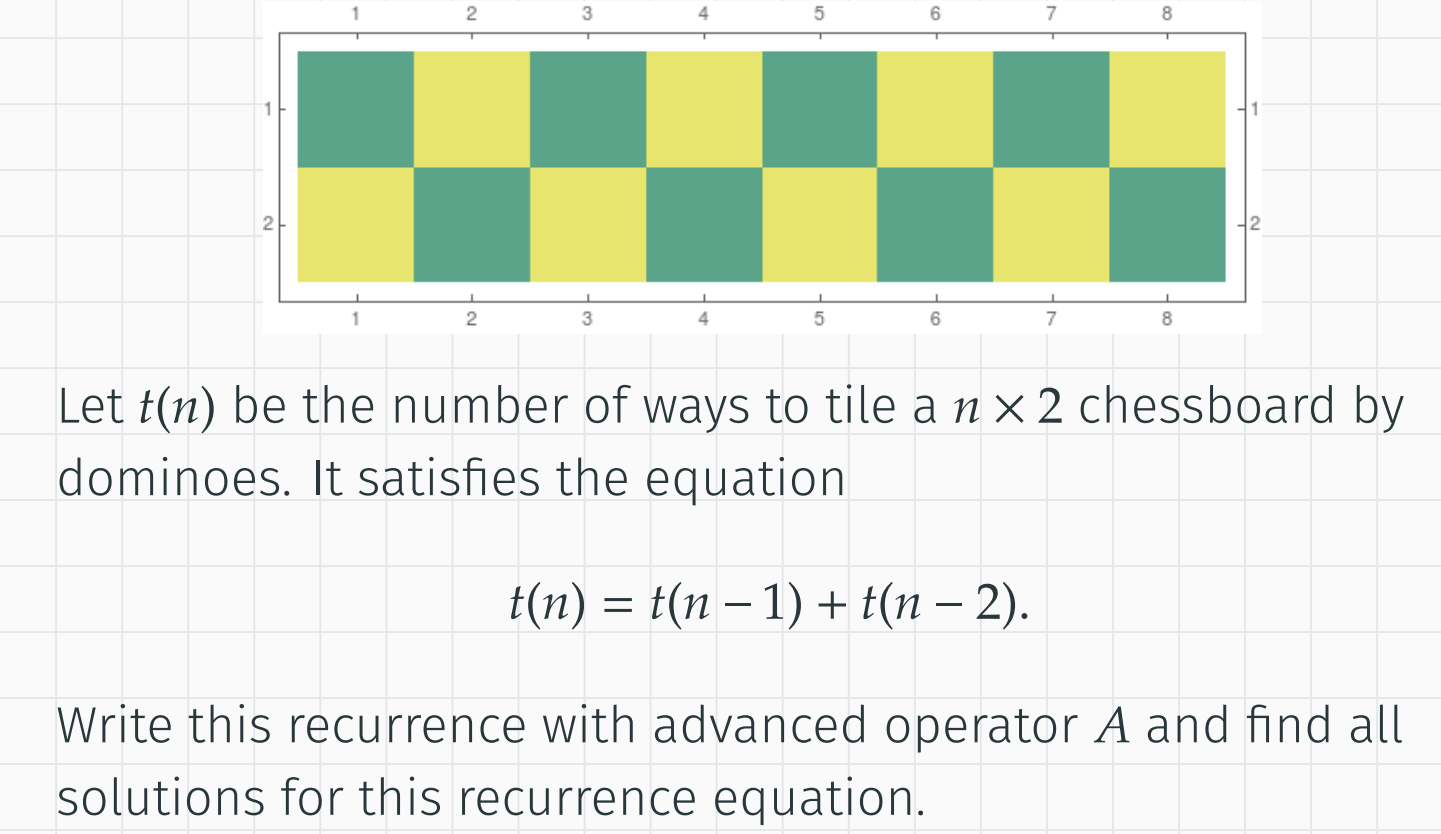
\includegraphics{0022}\newline
$$(A^2-A-1)=0$$
$$(A-\frac{1+\sqrt(5)}{2})(A-\frac{1-\sqrt(5)}{2})=0$$
\paragraph{Example 9.12}
Can we find all solutions to $$(A-2)^2f=0$$
Why $c_12^n+c_22^n$ probably does not give all the solutions?\newline
What if we try $c_2n2^n$
$$(A-2)c_2n2^n=c_2(n+1)2^{n+1}-c_2n2^{n+1}=c_22^{n+1}$$
\subsubsection{Exercises}
\paragraph{9.9.1}
Write each of the following recurrence equations as advancement operator equations.\newline
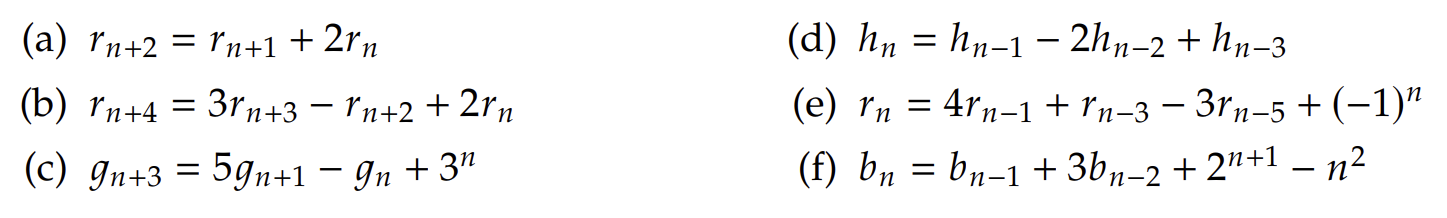
\includegraphics{0032}\newline
Solution:\newline
(a)$$(A^2 - A - 2)f = 0$$
(b)$$(A^4-3A^3+A^2-2)f=0$$
(c)$$(A^3-5A+1)f=0$$
(d)$$(h^3-h^2+2h-1)f=0$$
(e)$$(A^5 - 4A^4 - A^2 + 3)f =(-1)^{n+1}$$
(f)$$(A^2-A-3)f=2^{n+1}-n^2$$
\paragraph{9.9.3}
Find the general solution of the recurrence equation
$$g_{n+2}=3g_{n+1}-2g_n$$
Solution:\newline
$$(A^2-3A+2)f=0$$
$$(A-2)(A-1)f=0$$
Hence, our solutions are $c_12^n$ and $c_21^n = c2$. Combining these to generate the entire family of solutions gives us the general solution $g_n=c_12^n+c_2$
\paragraph{9.9.5}
Find an explicit formula for the $n^{th}$ Fibonacci number $f_n$ (See Subsection 9.1.1.)\newline
Solution:\newline
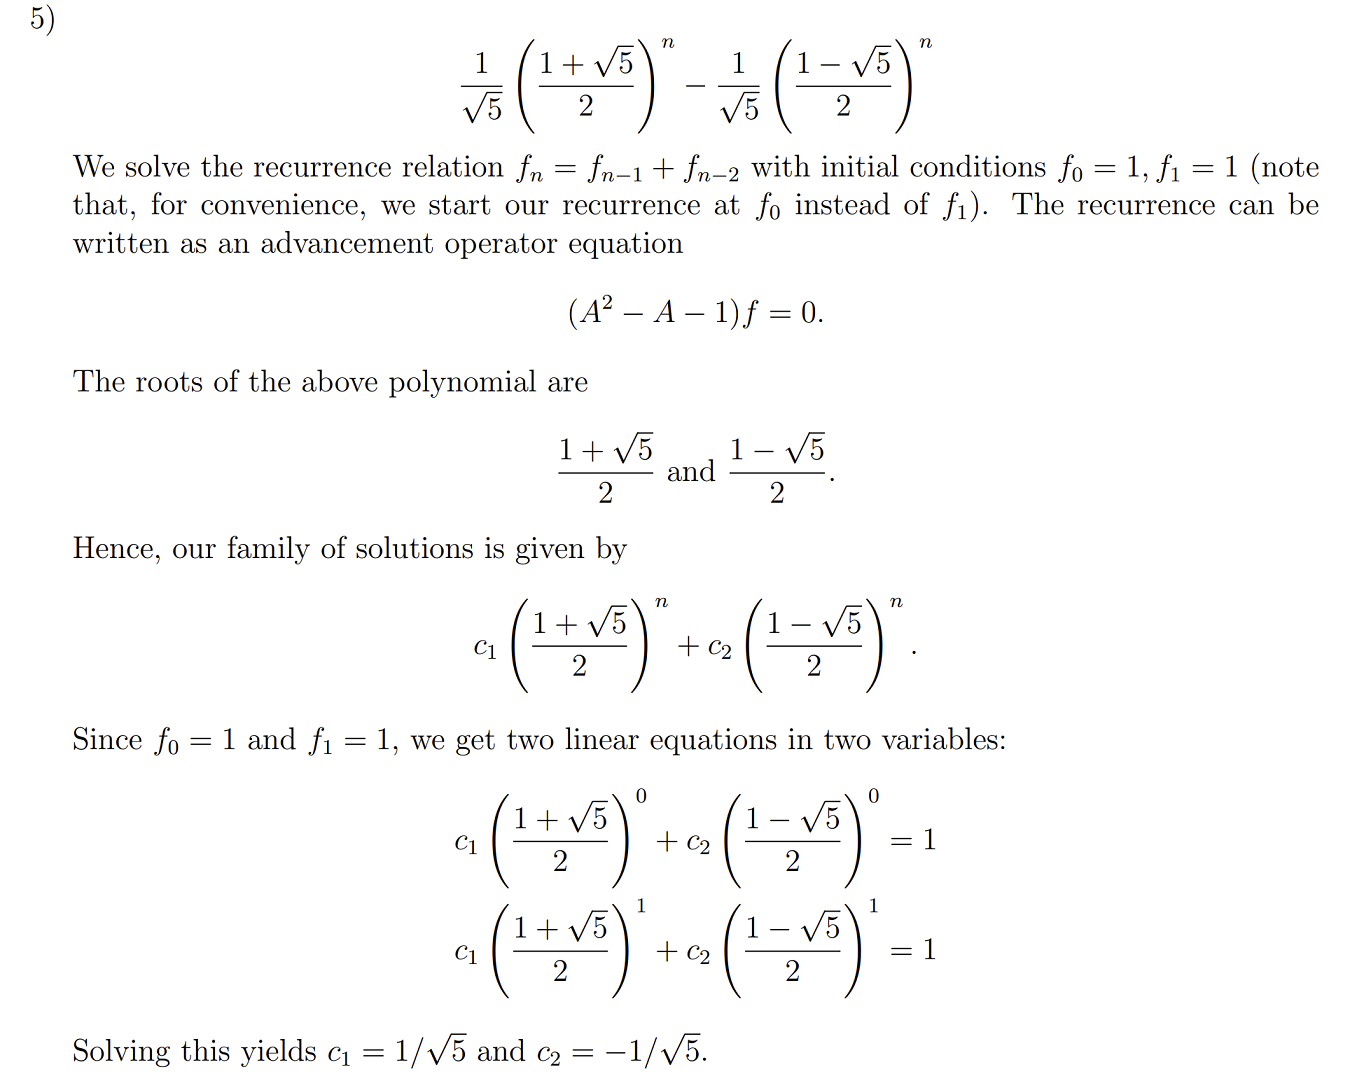
\includegraphics{0045}
\paragraph{9.9.7}
Solve the advancement operator equation $(A^2+3A-10)f=0$ if f(0)=2 and f(1)=10.\newline
Solution:\newline
$$(A^2+3A-10)f=(A+5)(A-2)$$
Such that
$$c_1(-5)^n+c_22^n$$ and we have f(0)=2 and f(1)=10
$$\begin{cases}
    {c_1+c_2=2}\\{-5c_1+2c_2=10}
\end{cases}$$
Solving this yields $c_1=-\frac{6}{7}, c_2=\frac{20}{7}$
\subsection{Lecture 15}
\subsubsection{Course material}
\paragraph{Nonhomogeneous equations}
Consider the homogeneous equation:$$(A+2)(A-6)f=0$$
What is the general solution for this $$f_1(n)=c_1(-2)^n+c_26^n$$
What is the general solution for $$(A+2)(A-6)f=3^n$$
No algorithm is known which grantees a solution of This.\newline
Experience suggests trying something look like the right
hand side (RHS), say, $de^n$, where d is to be decided.
$$(A-6)\cdot d3^n=A(d3^n)-6\cdot (d3^n)=d3^{n+1}-d\cdot 2\cdot 3^{n+1}=-d3^{n+1}$$
$$(A+2)\cdot (-d\cdot 3^{n+1})=A\cdot (-d3^{n+1})+2\cdot (-de^{n+1})=-d3^{n+2}-\frac{2}{3}d^3{n+2}=-\frac{5}{3}d\cdot 3^{n+2}=-15d3^n$$
Thus, we have$$3^n=-15d3^n$$
so we have 
$$d=-\frac{1}{15}$$
This gives one particular solution
$$f_2(n)=-\frac{3^n}{15}$$
All solutions of $f(n)=f_1(n)+f_2(n)$ are of this form - $$f(n)=f_1(n)+f_2(n)$$
e.g. $$c_1(-2)^n+c_26^n$$
$$(A+2)(A-6)(f_1+f_2)=(A+2)(A-6)f_1+(A+2)(A-6)f_2=0+3^n$$
So $f_1+f_2$ is a solution for $$(A+2)(A-6)f=3^n$$ is a solution $$(A+2)(A-6)f=3^n$$
\paragraph{The recipe for Nonhomogeneous equations}
We want to solve solution for 
$$p(A)f=g$$
First we find the general solution $f_1$ for
$$p(A)f=0$$
Second we find (any) particular solution (by guessing) $f_2$ for 
$$p(A)f=g$$
Then the general solution is
$$f(n)=f_1(n)+f_2(n)$$
Example 9.15:\newline
Find the solutions to the equation
$$(A+2)(A-6)=6^n$$
if $f(0)=1$ and $f(1)=5$
Solution:\newline
1.Solve $(A+2)(A-6)f=0$\newline
We can get solution:$f_1(n)=c_1(-2)^n+c_26^n$\newline
2.Find one solution for $(A+2)(A-6)f=6^n$\newline
We try to find a d such that $(A+2)(A-6)f=d6^n$.
$$Step1:\ (A-6)d6^n=d6^{n+1}-d6^{n+1}=0$$
$$Step2:\ (A+2)\cdot 0=0$$
Thus, it is impossible to get $d\cdot 6^n$ \newline
So we try $d\cdot n\cdot 6^n$
$$(A+2)(A-6)\cdot 6d^n\cdot 6^n=?$$
$$(A-6)\cdot dn6^n=d(n+1)6^{n+1}-dn6^{n+1}=d6^{n+1}((n+1)-n)=d6^{n+1}$$
$$(A+2)d6^{n+1}=d6^{n+2}+2d6^{n+1}=6^n\cdot 48d$$
To make this a solution, we want:
$$6^n48d=6^n$$
So we take $d=\frac{1}{48}$
Therefore, a particular solution is 
$$n6^nd=n\frac{6^n}{48}=f_2(n)$$
Thus, the final answer should be 
$$f_1(n)+f_2(n)=c_1(-2)^n+c_26^n+n\frac{6^n}{48}$$
Given that $f(0)=1,f(1)=5$\newline
Then we have 
$$b_n=\begin{cases}
    {c_1(-2)^0+c^26^0+0\cdot \frac{6^0}{48}=1}\\{c_1(-2)^1+c_26^1+1\cdot \frac{6^1}{48}=5}
\end{cases}$$
$$\begin{cases}
    {c_1+c_2=1}\\
    {-2c_1+6c_2+\frac{1}{8}=c}
\end{cases}$$
$$\begin{cases}
    {c_1=\frac{9}{64}}\\
    {c_2=\frac{55}{64}}
\end{cases}$$
Thus,$$f(n)=\frac{9}{64}(-2)^n+\frac{55}{64}6^n+\frac{n\cdot 6^n}{48}$$
\paragraph{Example 9.16}
Find all solutions to the equation
$$r_{n+1}r_n+n+1$$
$$r_{n+1}-r_n=n+1 \Longleftrightarrow (A-1)r_n=n+1$$
$$(A-1)r_n=0$$
Step1: The solution of $f_1(n)=c_1(1)^n=c_1$\newline
Step2: Find a particular solution for
$$(A-1)r_n=n+1$$
Guess =$d_1n^2+d_2n+d_3$
Thus,
$$(A-1)(d_1n^2+d^2n+d^3=d_1(n+1)^2+d^2(n+1)+d_3-(d_1n^2+d_2n+d^3))=2d_1n+d_1+d_2=n+1$$
$\Longrightarrow$
$$d_1=\frac{1}{2},d_2=\frac{1}{2}$$
Therefore, the solution will be
$$c_1+d_1n^2+d_2n+d_3$$
\subsubsection{Exercises}
\paragraph{9.9.9}
For each nonhomogeneous advancement operator equation, find its general solution.\newline
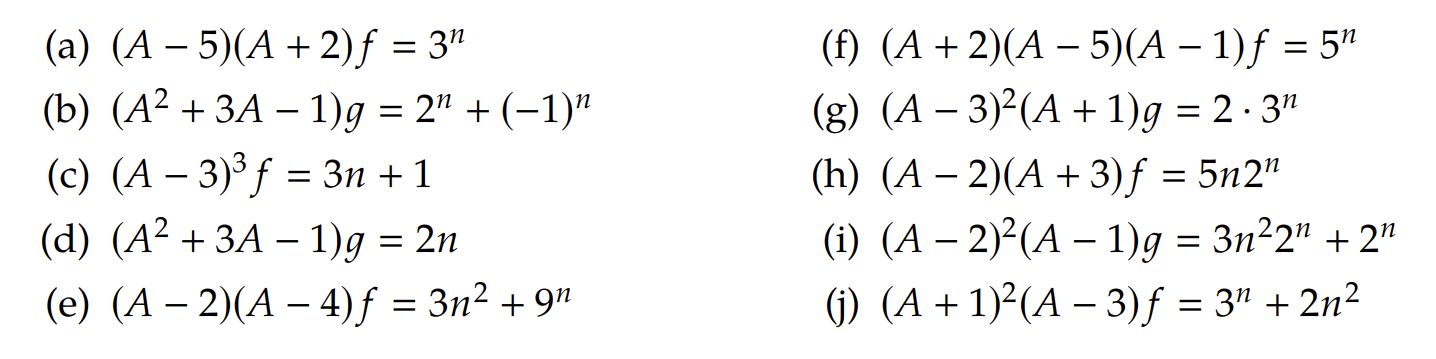
\includegraphics{0033}\newline
Solution:\newline
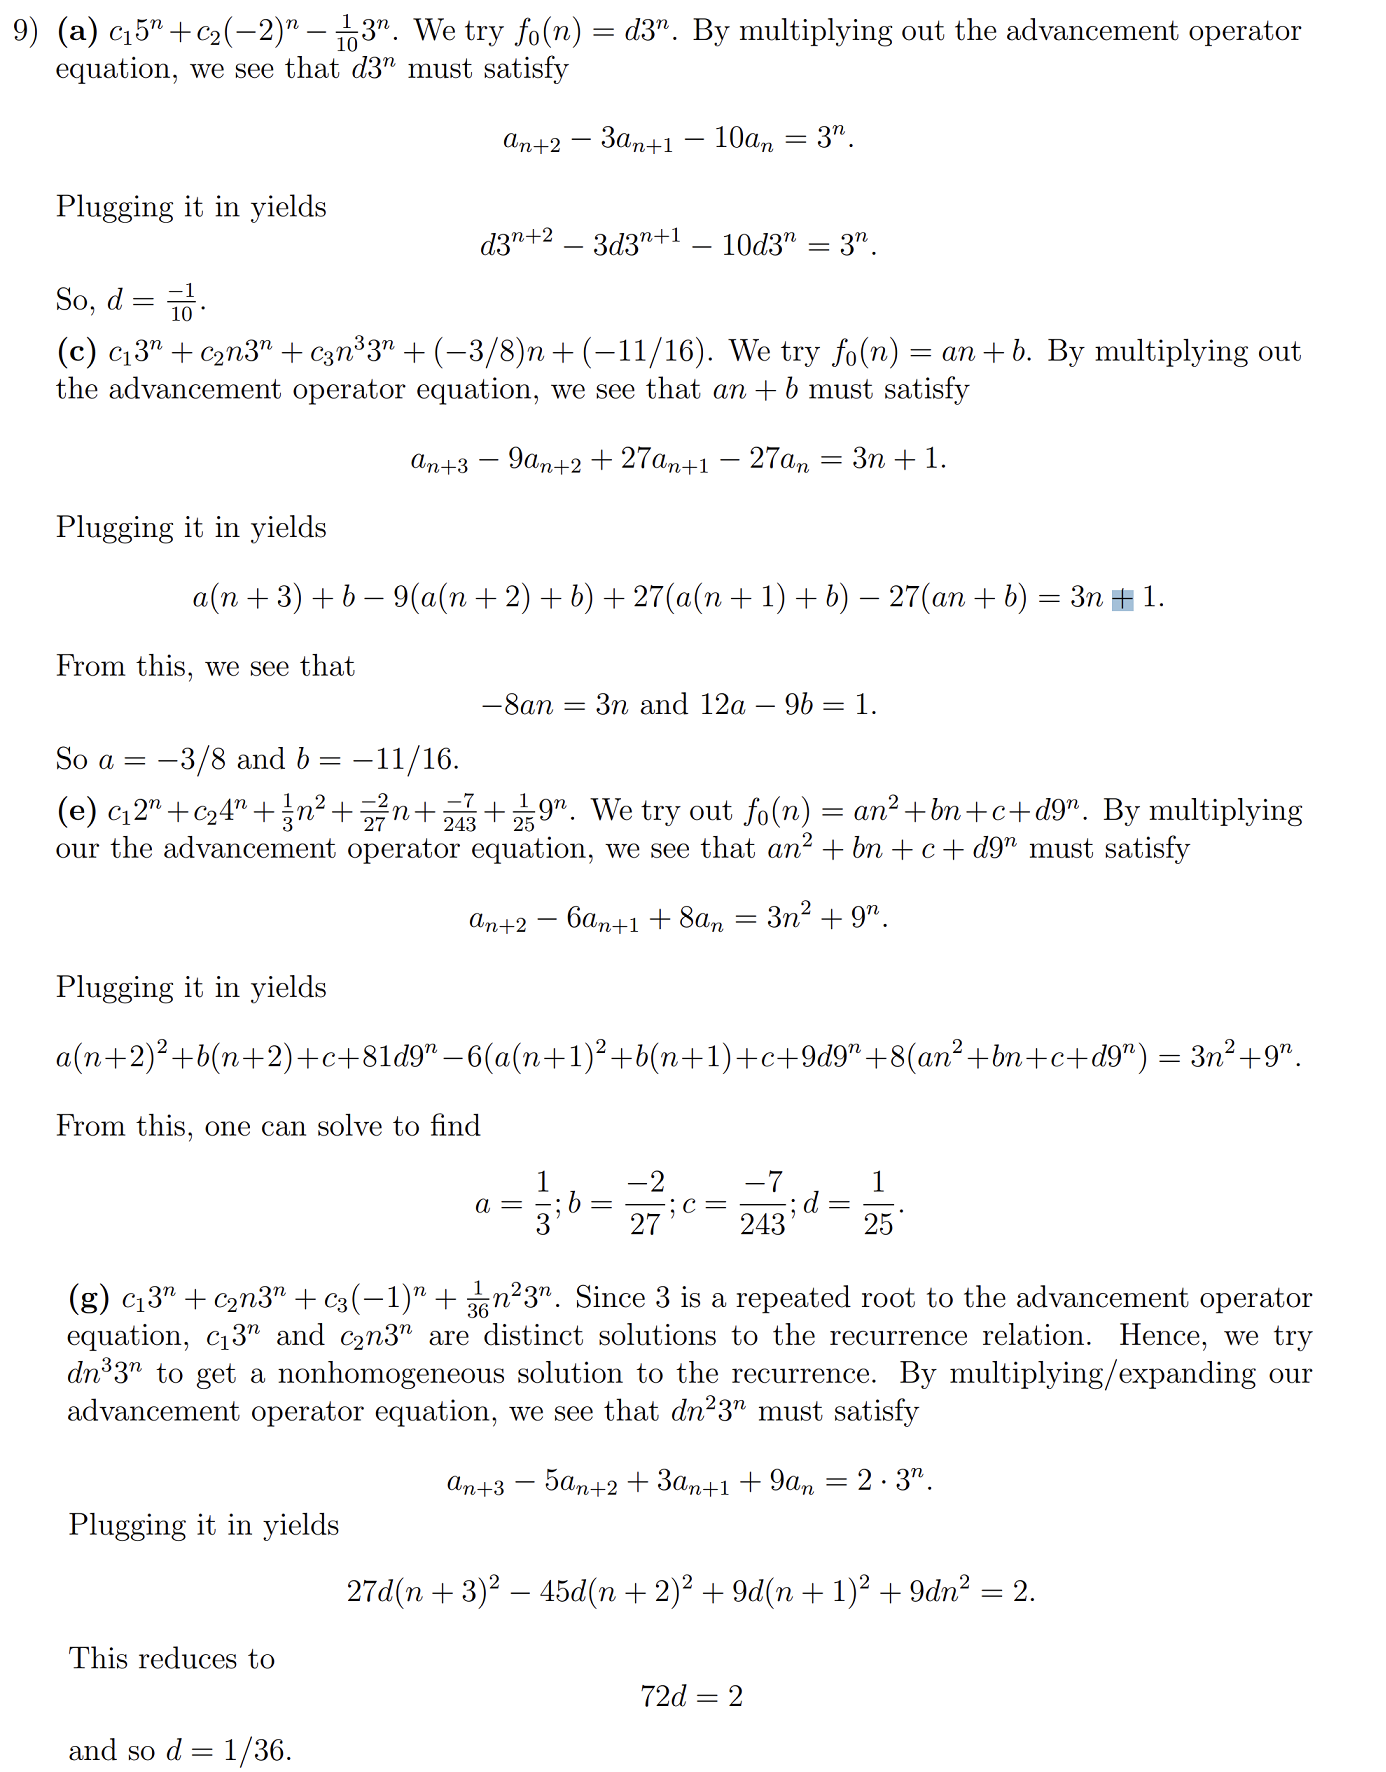
\includegraphics{0046}\newline
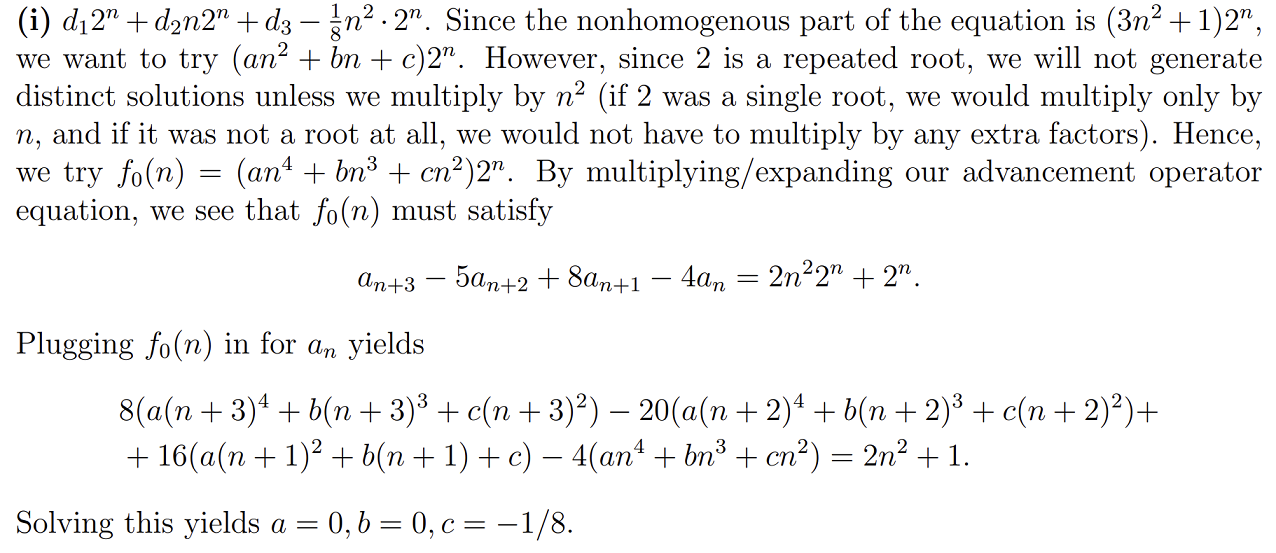
\includegraphics{0046-1}
\paragraph{9.9.11}
There is a famous puzzle called the Towers of Hanoi that consists of three pegs and n circular discs, all of different sizes. The discs start on the leftmost peg, with the largest disc on the bottom, the second largest on top of it, and so on, up to the smallest disc on top. The goal is to move the discs so that they are stacked in this same order on the rightmost peg. However, you are allowed to move only one disc at a time, and you are never able to place a larger disc on top of a smaller disc. Let $t_n$ denote the fewest moves (a move being taking a disc from one peg and placing it onto another) in which you can accomplish the goal. Determine an explicit formula for $t_n$.\newline
Solution:\newline
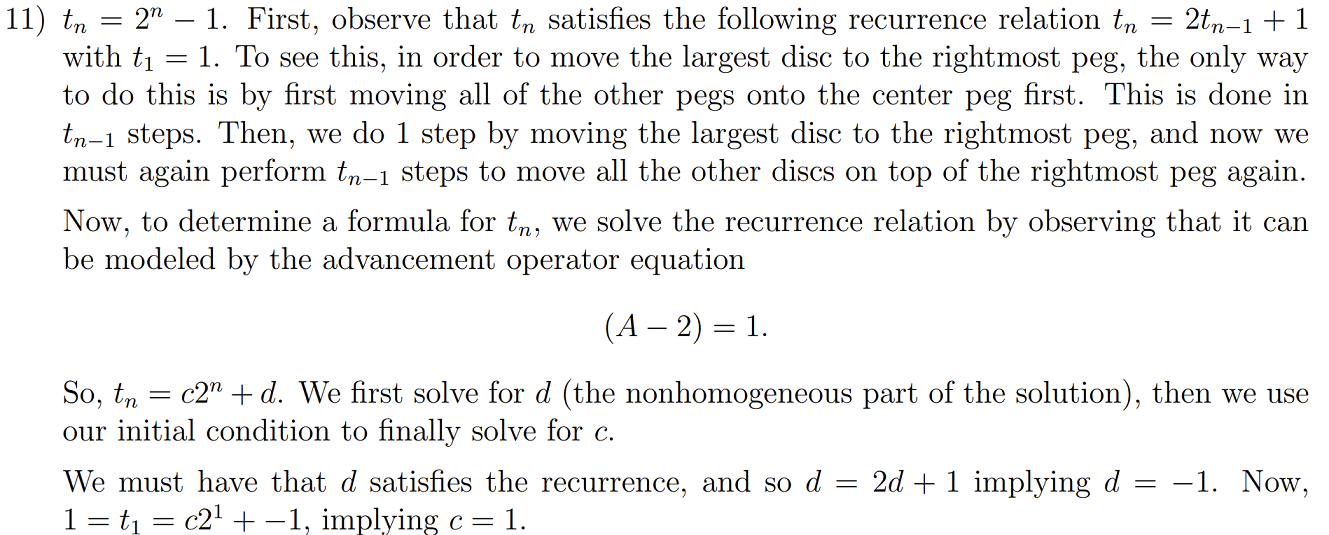
\includegraphics{0047}
\paragraph{9.9.13}
Let $t_n$ be the number of ways to tile a $2\times n$ rectangle using $1\times 1$ tiles and L-tiles. An
L-tile is a $2 \times 2$ tile with the upper-right $1 \times 1$ square deleted. (An L tile may be rotated so that the “missing” square appears in any of the four positions.) Find a recursive formula for $t_n$ along with enough initial conditions to get the recursion started. Use this recursive formula to find a closed formula for $t_n$.\newline
Solution:\newline
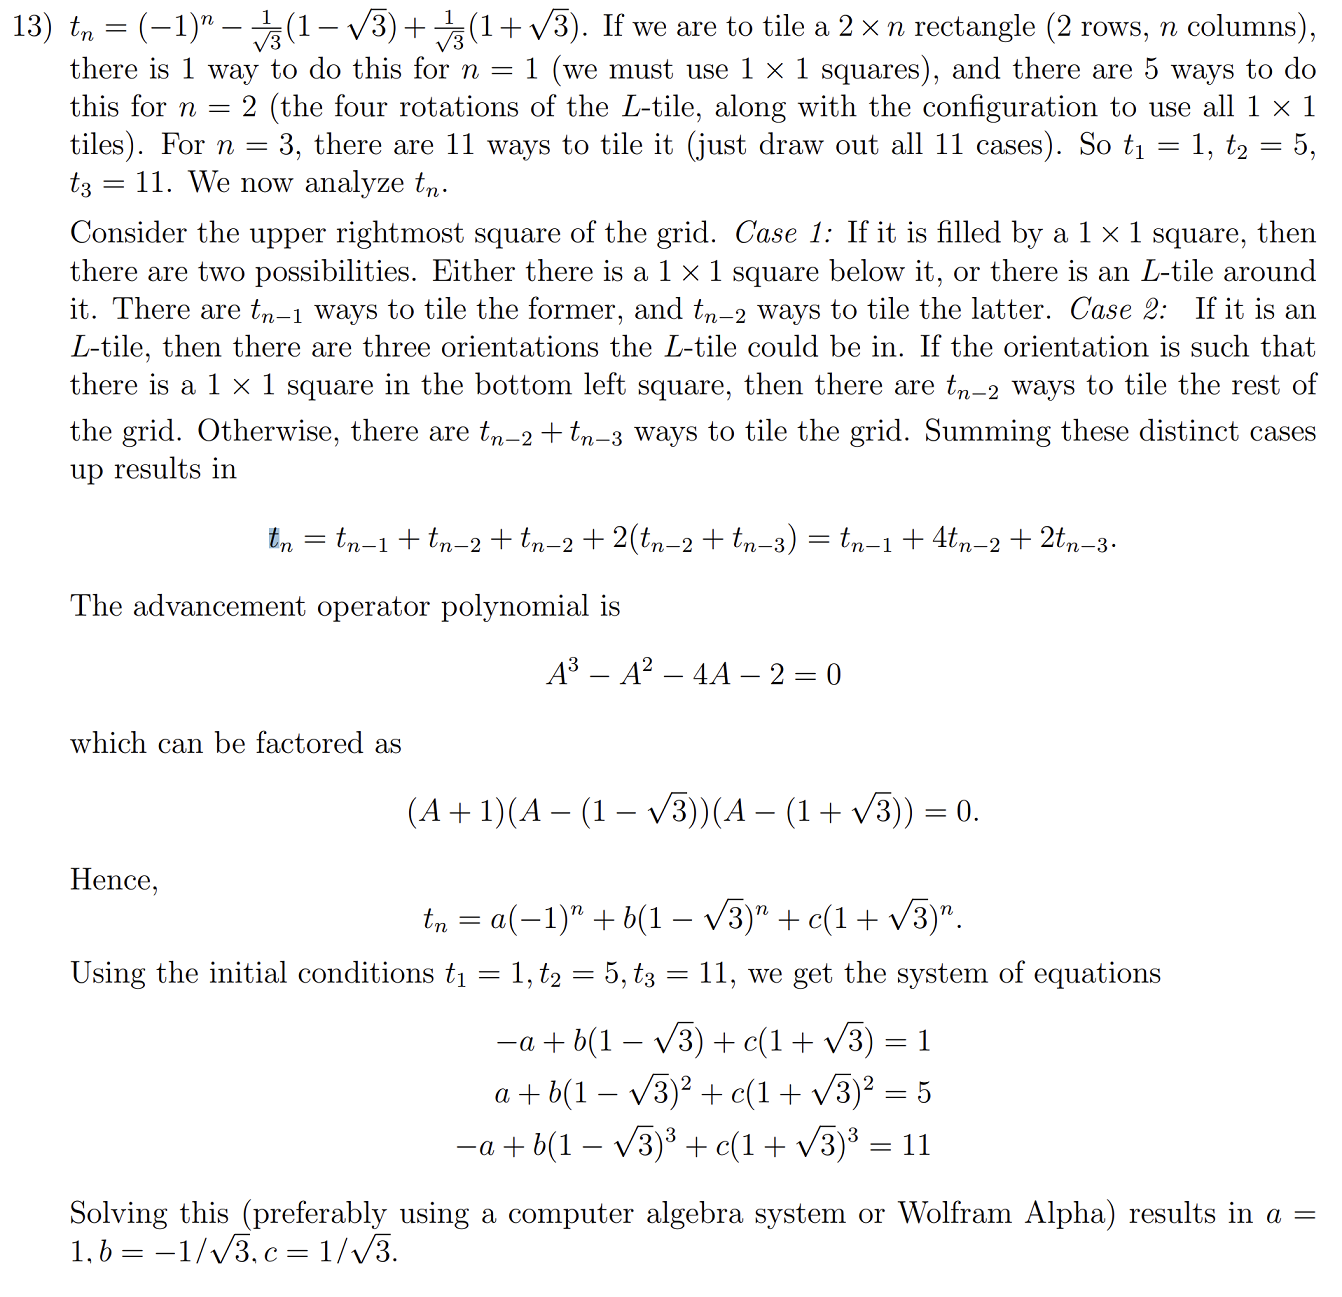
\includegraphics{0048}
\paragraph{9.9.15}
Use generating functions to solve the recurrence equation $r_n=r_{n-1}+6r_{n-2}$ for $n\ge 2$ with $r_0=1$, $r_1=3$.\newline
Solution:\newline
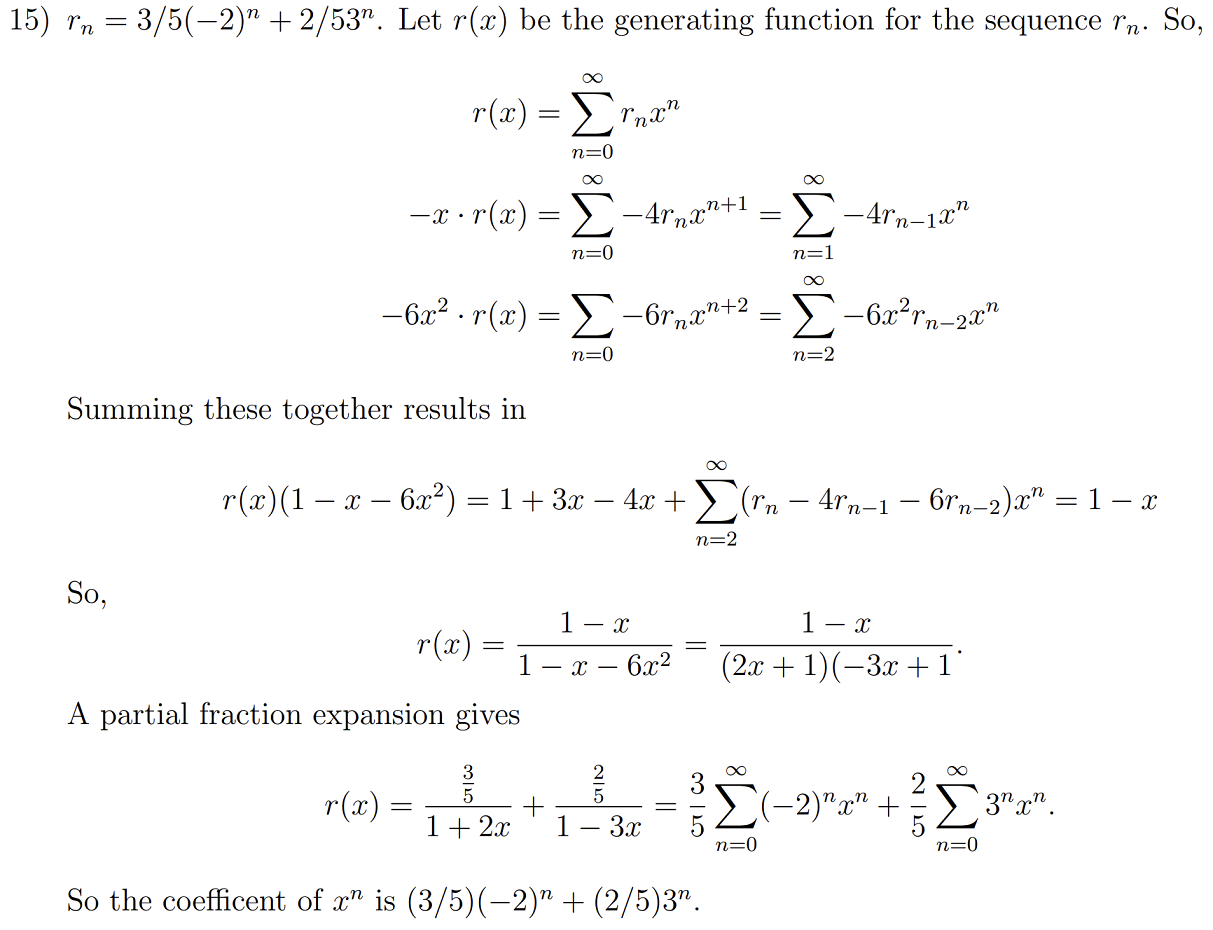
\includegraphics{0049}
\paragraph{9.9.17}
Let $b_0=1, b_2=1, b_3=4$. Use generating functions to solve the recurrence equation $b_{n+3}=4b_{n+2}-b_{n+1}-6b_n+3^n$ for $n\ge 0$\newline
Solution:\newline
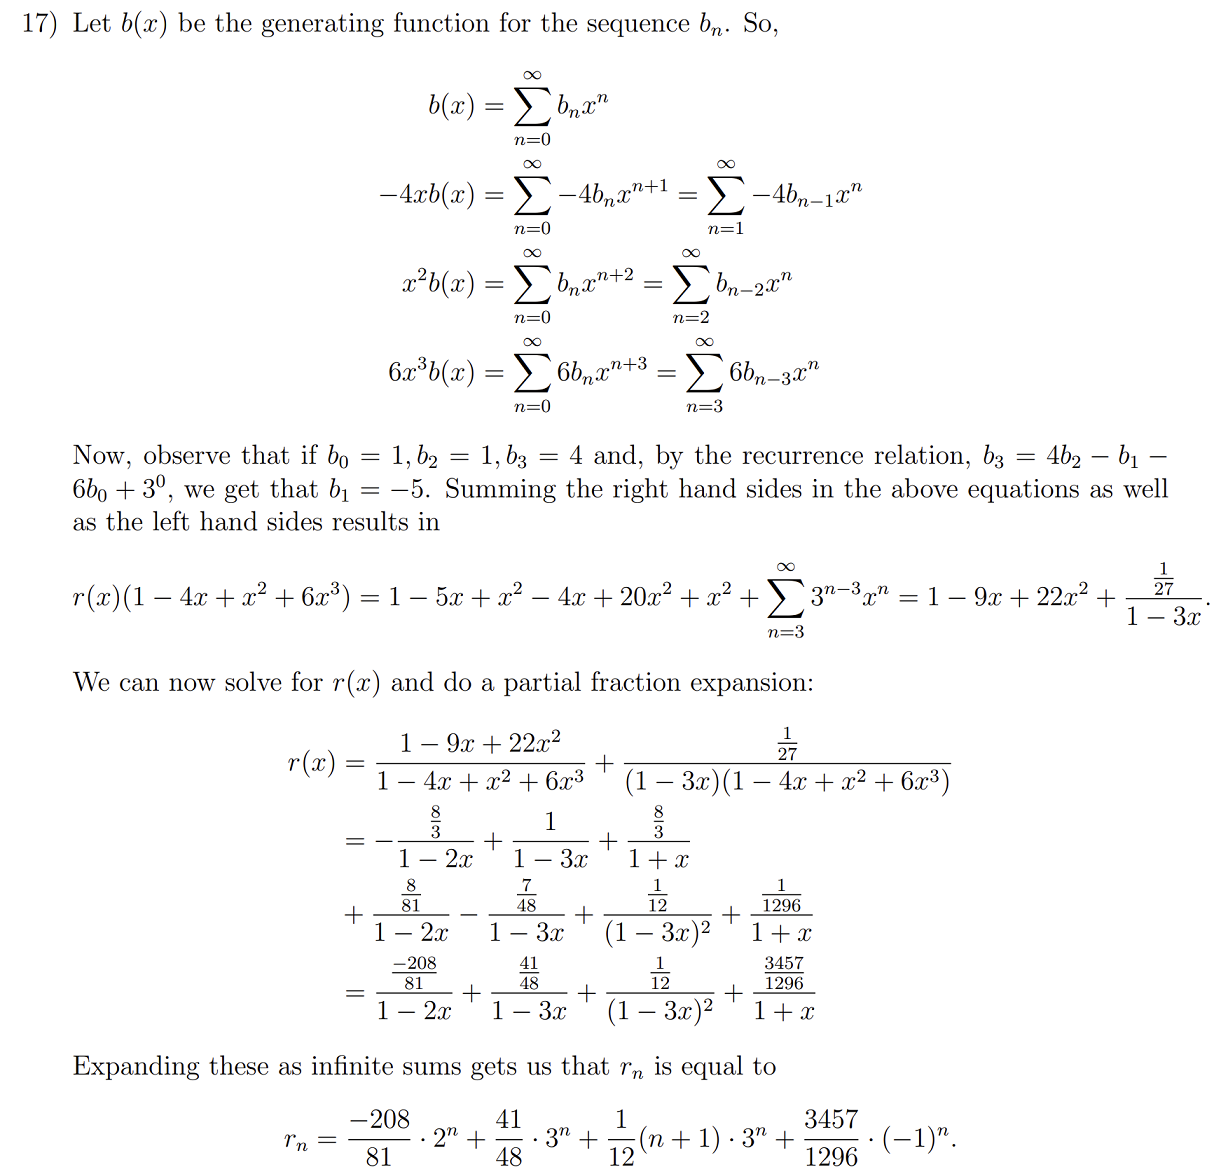
\includegraphics{0050}
\paragraph{9.9.19}
How many rooted, unlabeled, binary, ordered, trees (RUBOTs) with 6 leaves are there? Draw 6 distinct RUBOTs with 6 leaves.\newline
Hint:\newline
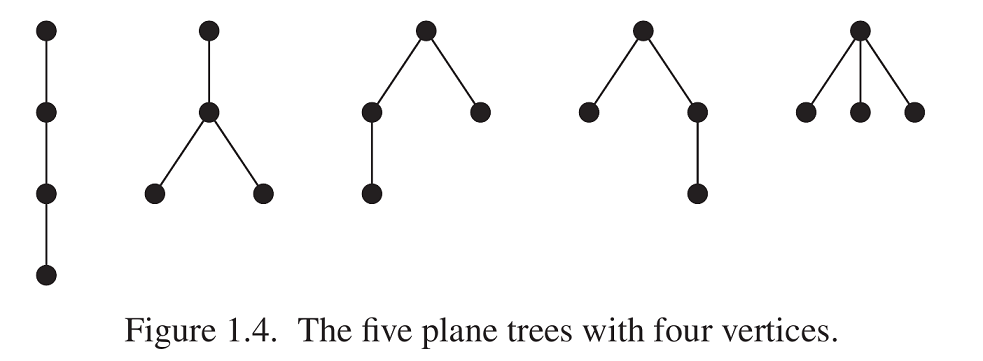
\includegraphics{0051}
Let $r_n$ be the number of RUBOTs of size $n$.
For example, $a_4=5$ as shown in the picture.\newline
Can you compute $a_1,a_2,a_3$\newline.
Search on https://OEIS.org with these numbers, you should get very a good guess of what is $a_6$.\newline
As for a proof, write down a recursion $R(x)=\sum_{n=0}^{\infty}a_nx^n$ should satisfy.\newline
See section 9.7 for an example of similar problem with Catalan numbers $C_n$
\subsection{Lecture 16}
\subsubsection{Course material}
\paragraph{Basic notations and terminologies for graphs:Basics}:\newline
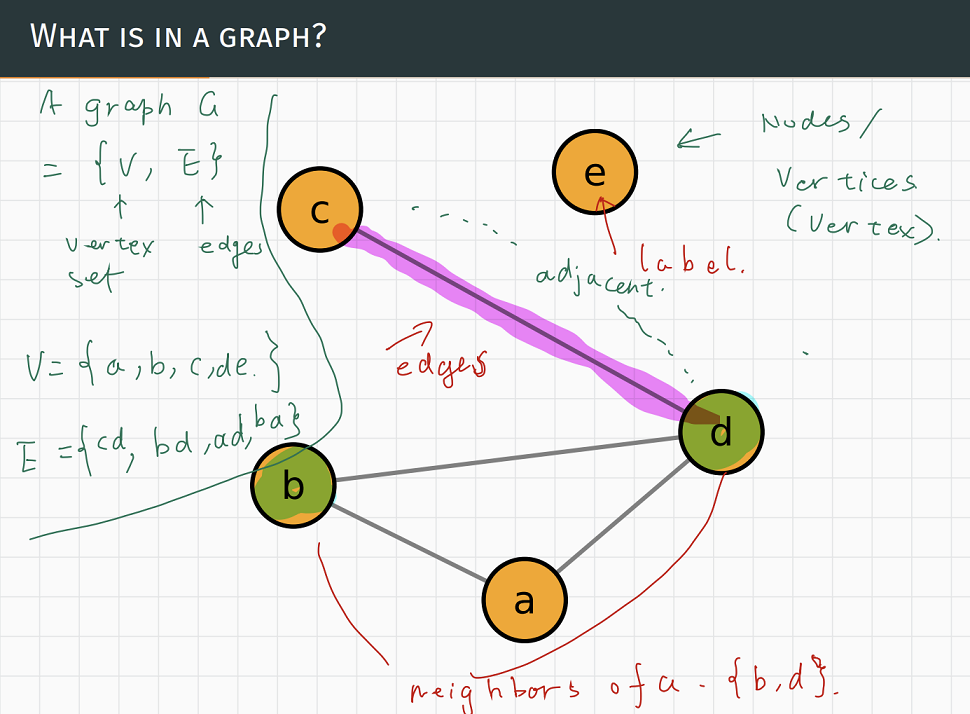
\includegraphics{0034}\newline
What is exactly a graph?\newline
\begin{lstlisting}
A graph G is a pair (V, E) .
V is a set and E is a set of 2-element subsets of V.
Elements of V are called vertices/nodes.
Elements of E are called edges.
We call V the vertex set of G and E is the edge set.
We abbreviate an edge {x, y} by xy.
If xy in E, we say x and y are adjacent, and the edge xy is
incident to x and y.
\end{lstlisting}
Let V=$\{a,b,c,d,e\}$. Let E=$\{\{a,b\},\{c,d\}\{a,d\}\{c,b\}\}$\newline
Which of the following are G=(V,E)?\newline
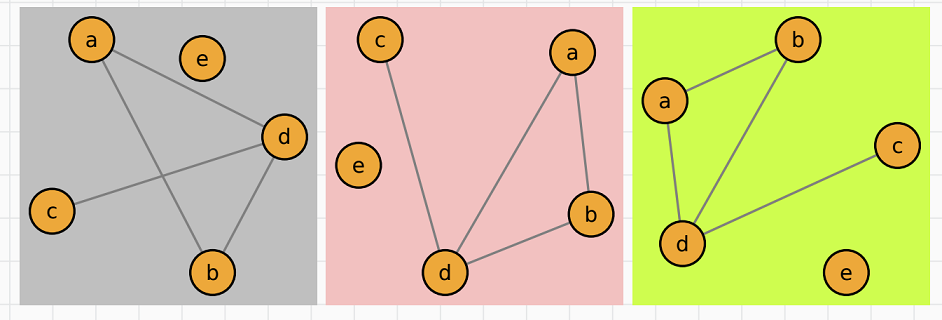
\includegraphics{0024}\newline
Answer: None of them.
\paragraph{Basic notations and terminologies for graphs:Neighbours}
The neighbourhood of a vertex x is the set of vertices adjacent to x.The degree of a vertex x in a graph G denoted $deg_G(v)$.is the number of vertices in its neighbourhood. \newline
What is the neighbourhood and degree of vertex 12?\newline
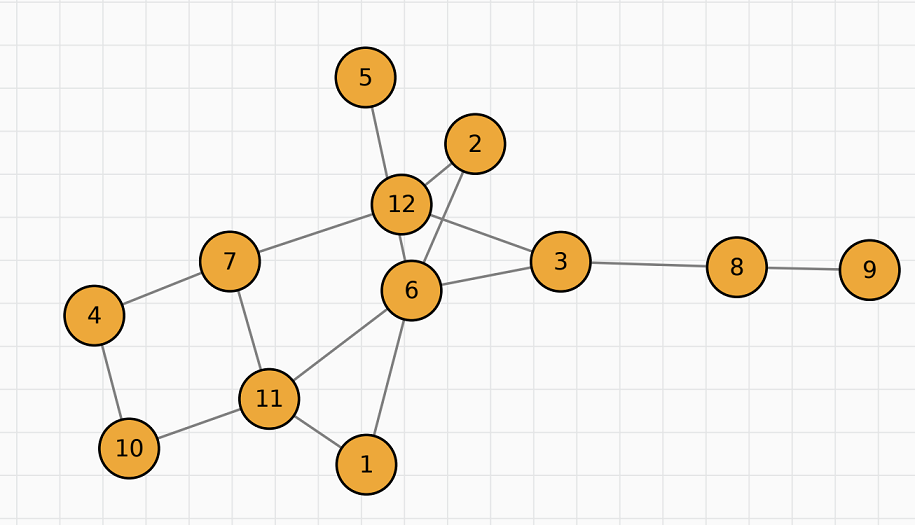
\includegraphics{0025}\newline
$deg_G(12)=5$
\paragraph{Subgraphs}
When G=(V,E) and H=(W,F) are graphs, we say H is a subgraph of G when $W\subseteq V$ and $F\subseteq E$.\newline
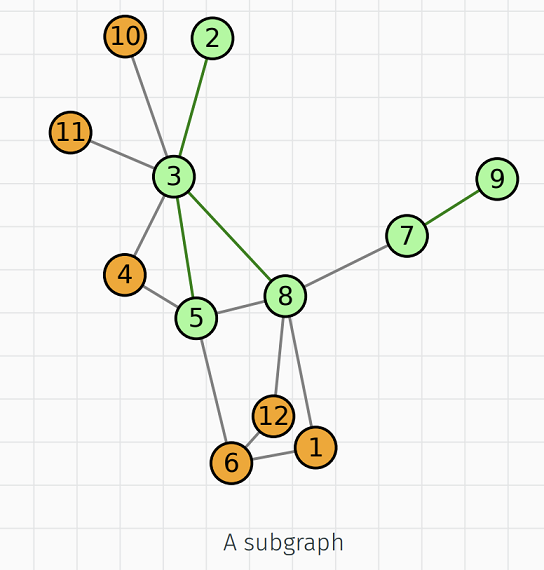
\includegraphics{0026}\newline
e.g. is $H=\{W=\{2,3,5\},F=\{23,35,34\}\}$ a subgraph?\newline
No, F is not a graph,
\paragraph{Spanning subgraphs}
A subgraph $H=(W,F)$, of $G=(V,E)$ is a spanning subgraph when W=V.
\paragraph{Induced subgraphs}
A subgraph $H=(W,F)$, of $G=(V,E)$ is a spanning subgraph if $xy\in E$ and $x,y\in W$ implies that $xy\in F$.\newline
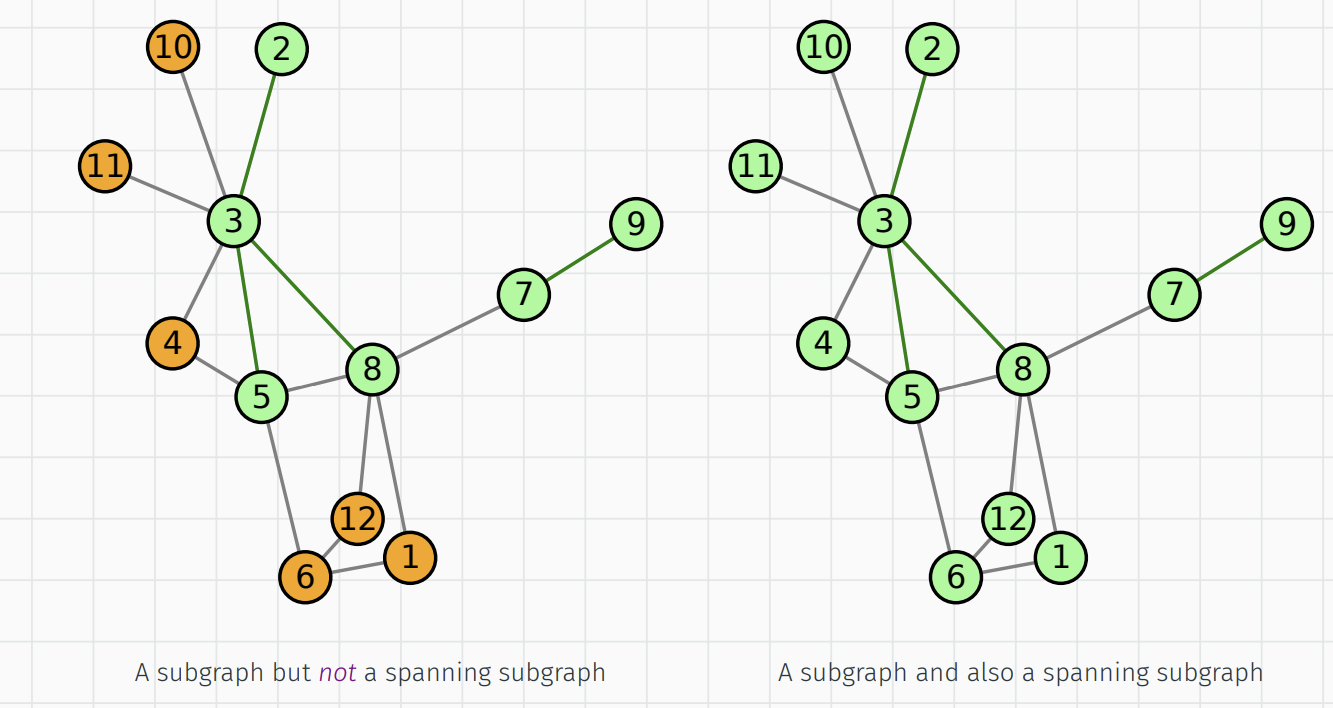
\includegraphics{0027}\newline
\paragraph{Complete graph}
A graph G=(V,E) is called a complete graph when $xy$ is an edge in G for every distinct pair $x,y\in V$.\newline
We let $K_n$ denote the complete graph with n vertices.\newline
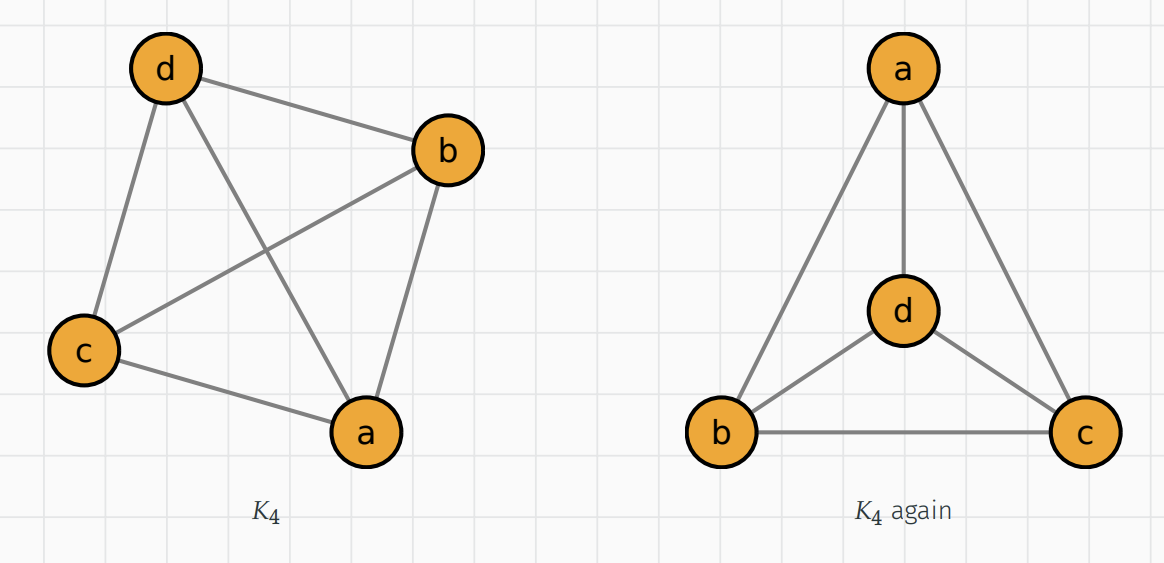
\includegraphics{0028}\newline
How many edges do $K_5$ have? $K_n$?\newline
Answer:$\binom{5}{2},\binom{n}{2}$
\paragraph{Independent graph}
A graph G=(V,E) is called a independent graph when xy is not an edge in G for every distinct pair $x,y\in V$\newline
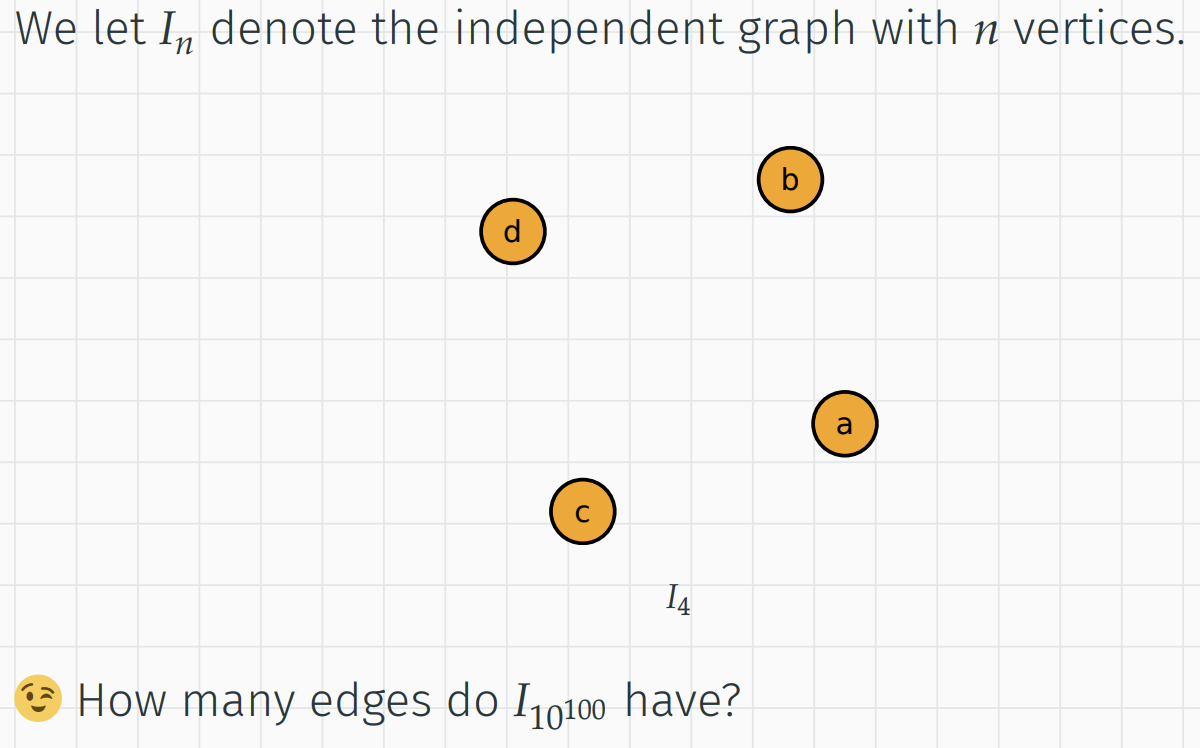
\includegraphics{0029}\newline
0
\paragraph{Walks} A sequence $(x_1,x_2,\cdots,x_n)$ of vertices in a graph G=(V,E) is called a walk when $x_ix_{i+1}$ is an edge for each $i\in [n-1]$\newline

\paragraph{Paths}
A walk which visits each vertex at most once is called a path.
\paragraph{Cycles}
A walk which starts and ends at the same vertex but visits only distinct vertices otherwise is called a cycle.
\paragraph{Graphs isomorphism}
Let $G=(V,E)$ and $H=(W,F)$ be two graphs.If there is way to relabel G's vertices to get H, then we say G is isomorphic to H.\newline
\includegraphics{0030}
\paragraph{Connected graphs}
A graph G is connected when there is a path from x to y, for every $x,y\in V$; Otherwise, we say G is disconnected.\newline
We call a maximal connected subgraph of G a component.\newline
\includegraphics{0031}
\paragraph{Proof of Theorem 5.9 (AC)}
Let $deg_G(v)$ denote the degree of vertex v in graph $G=(V,E)$. Then,
$$\sum_{v\in V}deg_G(v)=2|E|$$
Argument:\newline
The LHS counts each edge twice.
\paragraph{Corollary 5.10}
For any graph, the number of vertices of odd degree is even.\newline
Proof:\newline
We have $$\sum_{v\in V}deg_G(v)=2|E|$$
such that
$$\sum_{v:deg(v)\ is odd}deg(v)+\sum_{v:deg(v)\ is even}deg(v)$$.
Assume that G has odd number of vertices with odd degrees. This means LHS is odd. This is a contradiction.

\paragraph{Trees, forests and leaves}:\newline
A graph is acyclic when it does not contain any cycle.\newline
A connected acyclic graph is called a tree.\newline
Acyclic graphs are also called forests.\newline
Note that: Not to confuse the graph-theory tree with binary trees in combinatorics.
\paragraph{Spanning Trees}
For G = (V, E), a subgraph H = (W, F) of G is called a spanning tree if H is both a spanning subgraph of G and a tree.
\paragraph{Cut-edge}
An edge in a connected graph G is a cut-edge if removing it disconnects the graph.\newline
For example, the edges $\{9, 8\}, \{3, 8\}, \{5, 6\}$ are all cut-edges in the following graph.\newline
\includegraphics{0035}
\paragraph{Multigraphs: Loops and Multiple Edges}
An edge with both endpoints the same is called a loop.\newline
A graph in which loops and multiple edges between two vertices are allowed is calla a multigraph; otherwise it is called a simple graph.\newline
Note that:  In our course, a graph means a simple graph unless otherwise specifed.
\subsubsection{Exercises: Applied Combinatorics (AC)}
\paragraph{5.9.1}
The questions in this exercise pertain to the graph G shown in Figure 5.46.\newline
\includegraphics{0036}\newline
(a) What is the degree of vertex 8?\newline
(b) What is the degree of vertex 10?\newline
(c) How many vertices of degree 2 are there in G?
List them.\newline
(d) Find a cycle of length 8 in G.\newline
(e) What is the length of a shortest path from 3 to
4?\newline
(f) What is the length of a shortest path from 8 to
7?\newline
(g) Find a path of length 5 from vertex 4 to vertex 6.\newline
Solution:\newline
(a) 2.\newline
(b) 4.\newline
(c) There are five vertices of degree two. They are 1, 4, 6, 8, 9.\newline
(d) One cycle of length 8 is 1, 5, 6, 2, 3, 10, 4, 7, 1. There are others.\newline
(e) The length of the shortest path is two: 3, 10, 4. It cannot be length one since $\{3, 4\}$ is not
an edge.\newline
(f) The length of the shortest path is three. One such path is 8, 3, 2, 7. It cannot be length\newline
one since 8 is not adjacent to 7. It cannot be length two since no vertex in the neighborhood
of 8 is adjacent to 7.\newline
(g) Such a path is given by 4, 7, 1, 5, 2, 6.
\paragraph{5.9.3}
Draw a graph with 6 vertices having degrees 5, 4, 4, 2, 1, and 1 or explain why such
a graph does not exist.\newline
Solution:\newline
Such a graph cannot exist since by corollary 5.10, it must have an even number of odd degree
vertices. This graph would have three odd degree vertices which is a contradiction.
\paragraph{5.9.5}
For this exercise, consider the graph G in Figure 5.47.\newline
(a) Let $V_1$ = $\{g, j, c, h, e, f \}$ and $E_1$ = ${ge, jg, ch, ef }$. Is $(V_1, E_1)$ a subgraph of G?
(b) Let $V_2$ = $\{g, j, c, h, e, f \}$ and $E_2$ = $\{ge, j1, ch, ef , cj\}$. Is $(V_2, E_2)$ a subgraph of G?
(c) Let $V_3$ = $\{a, d, c, h, b\}$ and $E_3$ = $\{ch, ac, ad, bc\}$. Is $(V_3, E_3)$ an induced subgraph of G?\newline
(d) Draw the subgraph of G induced by $\{1, j, d, a, c, i\}$.\newline
(e) Draw the subgraph of G induced by $\{c, h, f , i, j\}$.\newline
(f) Draw a subgraph of G having vertex set $\{e, f , b, c, h, j\}$ that is not an induced subgraph.\newline
(g) Draw a spanning subgraph of G with exactly 10 edges.\newline
\includegraphics{0038}
Solution:\newline
(a) Yes.\newline
(b) No. $\{c, j\}$ is not an edge in G.\newline
(c) No. It must have edge {h, d} to be an induced subgraph of G\newline
\paragraph{5.9.7}
Figure 5.48 contains four graphs on six vertices. Determine which (if any) pairs of graphs are isomorphic. For pairs that are isomorphic, give an isomorphism between the two graphs. For pairs that are not isomorphic, explain why.\newline
\includegraphics{0039}\newline
Solution:\newline
$G_1$ and $G_3$ are isomorphic
\subsubsection{Exercises: Discrete Mathematics (DM)}
\paragraph{4.1.1}
If 10 people each shake hands with each other, how many handshakes took place? What does this question have to do with graph theory?\newline
Solution:\newline
This is asking for the number of edges in K10. Each vertex (person)
has degree (shook hands with) 9 (people). So the sum of the degrees is 90.
However, the degrees count each edge (handshake) twice, so there are 45
edges in the graph. That is how many handshakes took place.
\paragraph{4.1.2}
Among a group of 5 people, is it possible for everyone to be friends with exactly 2 of the people in the group? What about 3 of the people in the group?\newline
Solution:\newline
It is possible for everyone to be friends with exactly 2 people. You
could arrange the 5 people in a circle and say that everyone is friends with
the two people on either side of them (so you get the graph $C_5$). However,
it is not possible for everyone to be friends with 3 people. That would lead
to a graph with an odd number of odd degree vertices which is impossible
since the sum of the degrees must be even
\paragraph{4.1.3}
Is it possible for two different (non-isomorphic) graphs to have the same number of vertices and the same number of edges? What if the degrees of the vertices in the two graphs are the same (so both graphs have vertices with degrees 1, 2, 2, 3, and 4, for example)? Draw two such graphs or explain why not.\newline
Solution:\newline
No. This is impossible due to Euler’s formula.
\paragraph{4.1.4}
Are the two graphs below equal? Are they isomorphic? If they are isomorphic, give the isomorphism. If not, explain.\newline
\includegraphics{0040}\newline
Solution:\newline
The graphs are not equal. For example, graph 1 has an edge {a, b}
but graph 2 does not have that edge. They are isomorphic. One possible
isomorphism is $f: G_1 \to G_2$ defined by $f(a)=d, f(b)=c, f(c)=e, f(d)=b, f(e)=a.$
\paragraph{4.1.6}
What is the largest number of edges possible in a graph with 10 vertices? What is the largest number of edges possible in a bipartite graph with 10 vertices? What is the largest number of edges possible in a tree with 10 vertices?\newline
Hint:\newline
The bipartite graph is a little tricky. You will definitely want a
complete bipartite graph, but it could be $K_{5,5}$ or maybe $K_{1,9}$
\paragraph{4.1.7}
Which of the graphs below are bipartite? Justify your `answers.\newline
\includegraphics{0041}\newline
Solution:\newline
The first graph is bipartite, which can be seen by labeling it as follows.\newline
\includegraphics{0052}\newline
Two of the remaining three are also bipartite.
\paragraph{4.1.8}
For which n $\ge$ 3 is the graph $C_n$ bipartite?
Solution:\newline
$C_4$ is bipartite; $C_5$ is not.What about all the other values of n?
\paragraph{4.1.9}
For each of the following, try to give two different unlabeled graphs
with the given properties, or explain why doing so is impossible.\newline
(a) Two different trees with the same number of vertices and the
same number of edges. A tree is a connected graph with no
cycles.\newline
(b) Two different graphs with 8 vertices all of degree 2.\newline
(c) Two different graphs with 5 vertices all of degree 4.\newline
(d) Two different graphs with 5 vertices all of degree 3.\newline
Solution:\newline
(a) For example:\newline
\includegraphics{0053}\newline
(b) This is not possible if we require the graphs to be connected. If not,
we could take $C_8$ as one graph and two copies of $C_4$ as the other.\newline
(c) Not possible. If you have a graph with 5 vertices all of degree 4, then
every vertex must be adjacent to every other vertex. This is the graph
K5.\newline
(d) This is not possible. In fact, there is not even one graph with this
property (such a graph would have 5 · 3/2  7.5 edges).\newline
\paragraph{4.1.10}
Decide whether the statements below about subgraphs are true or
false. For those that are true, briefly explain why (1 or 2 sentences).
For any that are false, give a counterexample.\newline
(a) Any subgraph of a complete graph is also complete.\newline
(b) Any induced subgraph of a complete graph is also complete.\newline
(c) Any subgraph of a bipartite graph is bipartite.\newline
(d) Any subgraph of a tree is a tree.\newline
Solution:\newline
(a) False. (b) True. (c) True. (d) False.
\paragraph{4.1.11}
Let $k_1,k_2,\cdots,k_j$ be a list of positive integers that sum to n (i.e. $\sum_{i=1}^{j}k_i=n.$) Use two graphs containing n vertices to explain why:
$$\sum_{i=1}^j\binom{k_i}{2}\ge \binom{n}{2}$$\newline
Hint:\newline
How many edges does Kn have? One of the two graphs will not
be connected (unless j=1).
\paragraph{4.1.13}
A graph is a way of representing the relationships between elements
in a set: an edge between the vertices x and y tells us that x is related
to y (which we can write as x ~ y). Not all sorts of relationships can
be represented by a graph though. For each relationship described
below, either draw the graph or explain why the relationship cannot
be represented by a graph.\newline
(a) The set V = $\{1, 2, \cdots, 9\}$ and the relationship x ~ y when x - y
is a non-zero multiple of 3.\newline
(b) The set V = $\{1, 2, \cdots , 9\}$ and the relationship x ~ y when y is a
multiple of x.\newline
(c) The set V = $\{1, 2, \cdots , 9\}$ and the relationship x ~ y when
$0 < |x - y| < 3$\newline
Hint:\newline
Be careful to make sure the edges are not “directed.” In a graph, if
a is adjacent to b, then b is adjacent to a. In the language of relations, we
say that the edge relation is symmetric.
\paragraph{4.1.14}
Consider graphs with n vertices. Remember, graphs do not need to be
connected.\newline
(a) How many edges must the graph have to guarantee at least one
vertex has degree two or more? Prove your answer.\newline
(b) How many edges must the graph have to guarantee all vertices
have degree two or more? Prove your answer\newline
Hint:\newline
You might want to answer the questions for some specific values
of n to get a feel for them, but your final answers should be in terms of n.
\paragraph{4.1.15}
Prove that any graph with at least two vertices must have two vertices
of the same degree.\newline
Hint:\newline
Try a small example first: any graph with 8 vertices must have two
vertices of the same degree. If not, what would the degree sequence be?
\paragraph{4.1.16}
Suppose G is a connected graph with n$ > $1 vertices and n - 1 edges.
Prove that G has a vertex of degree 1. \newline
Hint:\newline
Use the handshake lemma 4.1.5. What would happen if all the
vertices had degree 2?\newline
\includegraphics{0054}
\newpage \section{Week5}
\subsection{Lecture 17}
\subsubsection{Course material}
\paragraph{Tree:Introduction}
Which of the following are trees and what about forest?\newline
\includegraphics{0055}\newline
1,2,6 are both tree and forest.\newline
\paragraph{Proposition 4.2.1}
A graph T is a tree if and only if between every pair of distinct vertices of T there is a unique path.\newline
e.g. T is a tree means T is connected and T has no cycle (T is a acyclic)\newline
\textbf{Proof:}\newline
T is connected means there is at least one path between two any vertices.\newline
To show uniqueness:\newline
we proof by contradiction.\newline
We assume that there are $u,v$ that there are 2 distinct path between them.\newline
\includegraphics{0059}\newline
\includegraphics{0060}
\paragraph{Corollary 4.2.2}
A graph F is a forest if and only if between any pair of vertices in F there is at most one path.\newline
\paragraph{Proposition 4.2.3 (DM) Proposition 5.11 (AC)}
Any tree with at least two vertices has at least two vertices of
degree one. Recall that such vertices are called leaves.\newline
Can we prove this by contradiction?\newline
\textbf{Prove}:\newline
Case1:\newline
Assume T is a tree with at least 2 vertices and T has lat most 2 leaves.\newline
Let P be the longest path in T.\newline
\includegraphics{0061}\newline
Then one of u,v has degree $\ge 2$. Let's say it's u\newline
\includegraphics{0062}\newline
case2:\newline
$u'\not\in v$ This is impossible because $p+u'$ is a longer path\newline
\paragraph{Proposition 4.2.4}
If T is a tree with v vertices and m edges, then $e=v-1$\newline
(Patch: Only one  vertice is still a tree)\newline
Proof:\newline
Base case:\newline $v=1,e=0.e=v-1$\newline
Induction case:\newline
Assume true for any tree with $v=k$\newline
We show that it's true for $v=k+1$\newline
Since $v=k+1\ge 2$, T has $\ge 2$ leaves.\newline
Let u be one of the two.\newline
Let u' be the neighbour of u, then remove the edge of uu'\newline
\includegraphics{0064}
\paragraph{A subtle point}
In both the proofs of Proposition 4.2.4 and 4.2.3, the induction
is done by deleting an edge from a larger tree.\newline
Why don’t we get a larger tree by adding an edge?\newline
\paragraph{TPS}
Can you show that every tree with average degree a i.e.,
$$\frac{\sum_{v\in V}deg(v)}{|V|}=a$$
has $\frac{2}{2-a}$ vertices?\newline
Recall that:\newline
A tree of $|V|$ vertices has  edges.\newline
$\sum_{v\in V}deg(v)=$
\subsubsection{Exercises}
\paragraph{4.2.1}
Which of the following graphs are trees?\newline
\includegraphics{0069}\newline
Solution:\newline
(a) This is not a tree since it contains a cycle. Note also that there are too
many edges to be a tree, since we know that all trees with v vertices
have $v - 1$ edges.\newline
(b) This is a tree since it is connected and contains no cycles (which you
can see by drawing the graph). All paths are trees.\newline
(c) This is a tree since it is connected and contains no cycles (draw the
graph). All stars are trees.\newline
(d) This is a not a tree since it is not connected. Note that there are not
enough edges to be a tree.\newline
\paragraph{4.2.2}
For each degree sequence below, decide whether it must always, must never, or could possibly be a degree sequence for a tree. Remember, a degree sequence lists out the degrees (number of edges incident to the vertex) of all the vertices in a graph in non-increasing order.\newline
(a) (4, 1, 1, 1, 1)\newline
(b) (3, 3, 2, 1, 1)\newline
(c) (2, 2, 2, 1, 1)\newline
(d) (4, 4, 3, 3, 3, 2, 2, 1, 1, 1, 1, 1, 1, 1)\newline
Solution:\newline
(a) This must be the degree sequence for a tree. This is because the
vertex of degree 4 must be adjacent to the four vertices of degree 1
(there are no other vertices for it to be adjacent to), and thus we get a
star.\newline
(b) This cannot be a tree. Each degree 3 vertex is adjacent to all but one
of the vertices in the graph. Thus each must be adjacent to one of
the degree 1 vertices (and not the other). That means both degree 3
vertices are adjacent to the degree 2 vertex, and to each other, so that
means there is a cycle.
Alternatively, count how many edges there are!\newline
(c) This might or might not be a tree. The length 4 path has this degree
sequence (this is a tree), but so does the union of a 3-cycle and a
length 1 path (which is not connected, so not a tree).\newline
(d) This cannot be a tree. The sum of the degrees is 28, so there are 14
edges. But there are 14 vertices as well, so we don’t have $v = e + 1$,
meaning this cannot be a tree.
\paragraph{4.2.3}
For each degree sequence below, decide whether it must always, must never, or could possibly be a degree sequence for a tree. Justify your answers.\newline
(a) (3, 3, 2, 2, 2)\newline
(b) (3, 2, 2, 1, 1, 1)\newline
(c) (3, 3, 3, 1, 1, 1)\newline
(d) (4, 4, 1, 1, 1, 1, 1, 1)\newline
Hint:\newline
Careful: the graphs might not be connected\newline
(a)(d) Possible, (b)(c) never.
\paragraph{4.2.4}Suppose you have a graph with v vertices and e edges that satisfies
$v = e + 1$. Must the graph be a tree? Prove your answer.\newline
Solution:\newline
Yes, the graph must be a tree.\newline
To prove this, we can use the fact that a tree is a connected graph with no cycles.\newline
Suppose the given graph is not a tree, meaning it has at least one cycle. Let C be a cycle in the graph. Since C is a cycle, it has at least 3 vertices and 3 edges. Let v be a vertex of C. Since the graph is connected, there exists a path P from v to some other vertex w that is not in C.\newline
Now, consider the graph G' obtained by removing the edge (v,w) from G. Since v and w are not in the same connected component of G', and since G is connected, there must be some other edge (u,x) in G that connects the connected components of v and w in G'.\newline
Let G'' be the graph obtained by adding the edge (v,w) to G'. Notice that G'' is also connected since we can travel from any vertex to any other vertex either along the cycle C or via the path P, and any vertex not in C is still connected to v or w via the edges in G'.\newline
Now, consider the number of vertices and edges in G''.\newline
Number of vertices in G'': v\newline
Number of edges in G'': e - 1\newline
Number of edges added to get from G' to G'': 1\newline
Total number of edges in G'': e\newline
Since G'' has the same number of vertices and edges as the given graph, we have:\newline
$v = e$\newline
But this contradicts the given condition $v = e + 1$. Therefore, our assumption that the given graph has a cycle must be false, and hence, the graph is a tree.
\paragraph{4.2.5}Prove that any graph (not necessarily a tree) with v vertices and e
edges that satisfies $v > e + 1$ will NOT be connected.\newline
Solution:\newline
To prove that any graph with $v$ vertices and $e$ edges that satisfies $v > e + 1$ is not connected, we will use proof by contradiction.
\newline
Suppose that the graph is connected. Then by the definition of a connected graph, there exists a path between any two vertices in the graph. Let $v_1$ and $v_2$ be two vertices in the graph, and let $p$ be a path between them.
\newline
Since the graph has $v$ vertices and $e$ edges, we know that the average degree of each vertex is $\frac{2e}{v}$. Therefore, there must be at least one vertex on the path $p$ that has degree less than 2. Let $v_0$ be the first vertex on the path $p$ that has degree less than 2, and let $v_{-1}$ and $v_1$ be the vertices immediately before and after $v_0$ on the path $p$.
\newline
Since $v_0$ has degree less than 2, it must be connected to at most one vertex that is not on the path $p$. Let $u$ be this vertex, if it exists. Then we can remove the vertex $v_0$ and its incident edge from the graph, and connect $v_{-1}$ and $v_1$ directly with the edge $(v_{-1}, v_1)$, resulting in a new graph with $v-1$ vertices and $e-1$ edges.
\newline
Now we have two cases:
\newline
Case 1: $u$ does not exist. In this case, we simply remove the vertex $v_0$ and its incident edge from the graph, resulting in a new graph with $v-1$ vertices and $e-1$ edges.
\newline
Case 2: $u$ exists. In this case, we remove the vertex $v_0$ and its incident edge from the graph, and add the edge $(v_{-1}, u)$ and $(v_1, u)$, resulting in a new graph with $v-1$ vertices and $e$ edges.
\newline
In either case, the new graph has $v-1$ vertices and at most $e-1$ edges. Therefore, we have:
$$v-1 > (e-1)+1$$
 \paragraph{4.2.6}
If a graph G with v vertices and e edges is connected and has$ v < e +1$,
must it contain a cycle? Prove your answer.\newline
Solution:\newline
Yes. We will prove the contrapositive. Assume G does not contain
a cycle. Then G is a tree, so would have $v = e + 1$, contrary to stipulation.
 \paragraph{4.2.7}
We define a forest to be a graph with no cycles.\newline
(a) Explain why this is a good name. That is, explain why a forest is
a union of trees.\newline
(b) Suppose F is a forest consisting of m trees and v vertices. How
many edges does F have? Explain.\newline
(c) Prove that any graph G with v vertices and e edges that satisfies
$v < e + 1$ must contain a cycle (i.e., not be a forest).\newline
(a) A forest is a good name because a forest is a collection of trees in the sense that it is a graph with no cycles. A tree is a connected graph with no cycles. Thus, a forest is a collection of trees where the trees are the connected components of the graph. In other words, a forest is the union of its trees.\newline
(b) Each tree in the forest has at most $v-1$ edges (since a tree with $v$ vertices has $v-1$ edges). Therefore, the maximum number of edges in the forest is $m(v-1)$. However, since the forest is a graph with $v$ vertices and no cycles, it must have exactly $v-m$ edges. To see why, note that the sum of the degrees of the vertices in the forest is equal to twice the number of edges, since each edge contributes 2 to the sum of the degrees. Since each tree in the forest has $v_i-1$ edges and $v_i$ vertices, the sum of the degrees in each tree is $2(v_i-1)$, and the sum of the degrees in the forest is $\sum_{i=1}^m 2(v_i-1) = 2v-2m$. Therefore, the number of edges in the forest is $\frac{1}{2}(2v-2m) = v-m$.\newline
(c) Suppose that $G$ is a graph with $v$ vertices and $e$ edges that does not contain a cycle. Then $G$ is a forest consisting of $c$ connected components, where $c \leq v$. Each connected component of $G$ is a tree. Therefore, each connected component has at most $v-1$ edges. Thus, the total number of edges in $G$ is at most $(v-1)c$.\newline
However, we know that $v < e+1$. Therefore,\newline
$$\frac{v-1}{e} < \frac{e}{e} = 1$$\newline
Multiplying both sides by $e$, we get:
$$v-1 < e$$
This implies that the total number of edges in $G$ is strictly less than $e$. This contradicts our previous inequality that the total number of edges in $G$ is at most $(v-1)c$. Therefore, our assumption that $G$ is a forest must be false, and hence $G$ must contain a cycle.
 \paragraph{4.2.8}
 Give a careful proof of Corollary 4.2.2: A graph is a forest if and only if there is at most one path between any pair of vertices. Use proof by contrapositive (and not a proof by contradiction) for both directions.\newline
 Corollary 4.2.2: A graph F is a forest if and only if between any pair of vertices
in F there is at most one path.\newline
Solution:\newline
We will prove both directions of the statement by contrapositive.
\newline
First direction: If a graph is not a forest, then there exist two vertices with more than one path between them.
\newline
Suppose that a graph $G$ is not a forest. Then $G$ contains at least one cycle. Let $u$ and $v$ be two vertices on this cycle. Since there is a cycle, there are at least two distinct paths between $u$ and $v$: one that follows the cycle in one direction and another that follows the cycle in the opposite direction. Therefore, if a graph is not a forest, then there exist two vertices with more than one path between them.
\newline
Second direction: If there are two vertices with more than one path between them, then the graph is not a forest.
\newline
Suppose that there exist two vertices $u$ and $v$ in a graph $G$ such that there are at least two distinct paths between them. Let $P$ and $Q$ be two such paths. If $P$ and $Q$ have no common edges, then $G$ contains a cycle, and hence it is not a forest. Otherwise, let $w$ be the first vertex at which $P$ and $Q$ diverge. Then, $P$ and $Q$ form a cycle when concatenated from $u$ to $w$ and back to $u$ along $P$ or $Q$, respectively. Hence, $G$ contains a cycle and is not a forest. Therefore, if there are two vertices with more than one path between them, then the graph is not a forest.
\newline
Combining the two directions, we conclude that a graph is a forest if and only if there is at most one path between any pair of vertices.
 \paragraph{4.2.9}
 Give a careful proof by induction on the number of vertices, that every tree is bipartite.\newline
Solution:\newline
We will prove by induction on the number of vertices $n$ that every tree with $n$ vertices is bipartite.\newline
Base case: For $n = 1$, the tree consists of a single vertex, which is vacuously bipartite.\newline
Inductive step: Assume that every tree with $n$ vertices is bipartite. Let $T$ be a tree with $n+1$ vertices, and let $u$ be a leaf of $T$ (i.e., a vertex with degree $1$).\newline
Since $u$ is a leaf, it is adjacent to exactly one other vertex, say $v$. Remove $u$ and the edge connecting $u$ to $v$ from $T$ to obtain a new tree $T'$ with $n$ vertices. By the inductive hypothesis, $T'$ is bipartite, so its vertices can be partitioned into two sets $V_1$ and $V_2$ such that every edge of $T'$ has one endpoint in $V_1$ and the other in $V_2$.\newline
Now, we can add $u$ back into $T$ and assign it to the opposite set from $v$ (i.e., if $u$ is in $V_1$, then $v$ is in $V_2$, and vice versa). Since $u$ has degree $1$, the only edge incident to $u$ is the edge connecting $u$ to $v$, and this edge connects vertices in different sets, so the bipartite property is preserved. Therefore, $T$ is also bipartite.\newline
By the principle of mathematical induction, we have shown that every tree is bipartite.
 \paragraph{4.2.10}
 Consider the tree drawn below\newline
 \includegraphics{0070}\newline
(a) Suppose we designate vertex e as the root. List the children,
parents and siblings of each vertex. Does any vertex other than
e have grandchildren?\newline
(b) Suppose e is not chosen as the root. Does our choice of root
vertex change the number of children e has? The number of
grandchildren? How many are there of each?\newline
(c) In fact, pick any vertex in the tree and suppose it is not the root.
Explain why the number of children of that vertex does not
depend on which other vertex is the root.\newline
(d) Does the previous part work for other trees? Give an example
of a different tree for which it holds. Then either prove that it
always holds or give an example of a tree for which it doesn’t.\newline
Hint:\newline
Let's say some vertex in some tree has degree 4. Now, when the tree becomes rooted, one of its neighbors will become its parent. What about its other neighbors? How many children would this vertex have?\newline
If e is the root, then b will have three children (a, c, and d), all
of which will be siblings, and have b as their parent. a will not have any
children.\newline
In general, how can you determine the number of children a vertex
will have, if it is not a root?\newline
Solution:\newline
\paragraph{4.2.12}
Unless it is already a tree, a given graph G will have multiple spanning
trees. How similar or different must these be?\newline
(a) Must all spanning trees of a given graph be isomorphic to each
other? Explain why or give a counterexample.\newline
(b) Must all spanning trees of a given graph have the same number
of edges? Explain why or give a counterexample.\newline
(c) Must all spanning trees of a graph have the same number of leaves
(vertices of degree 1)? Explain why or give a counterexample.\newline
Solution:\newline
(a) No, although there are graphs for which this is true. For example, K4
has a spanning tree that is a path (of three edges) and also a spanning
tree that is a star (with center vertex of degree 3).\newline
(b) Yes. For a fixed graph, we have a fixed number v of vertices. Any
spanning tree of the graph will also have v vertices, and since it is a
tree, must have $v - 1$ edges.\newline
(c) No, although there are graph for which this is true (note that if all
spanning trees are isomorphic, then all spanning trees will have
the same number of leaves). Again, $K_4$ is a counterexample. One
spanning tree is a path, with only two leaves, another spanning tree
is a star with 3 leaves.
\paragraph{4.2.14}
Give an example of a graph that has exactly 7 different spanning trees. Note, it is acceptable for some or all of these spanning trees to be isomorphic.\newline
Solution:\newline
One example of a graph that has exactly 7 different spanning trees is the complete graph K4, as shown below:
\begin{lstlisting}
  A---B
  |   |
  C---D
\end{lstlisting}
The 7 different spanning trees of K4 are:\newline
The tree with edges AB, AC, AD\newline
The tree with edges AB, BC, CD\newline
The tree with edges AB, BD, CD\newline
The tree with edges AC, BC, AD\newline
The tree with edges AC, BD, CD\newline
The tree with edges BC, BD, AD\newline
The tree with edges AB, BC, BD\newline
Note that some of these spanning trees may be isomorphic to each other. For example, the first spanning tree is isomorphic to the third and the seventh spanning trees, as they all have the same structure and only differ in the labeling of the nodes.
\paragraph{4.2.15}
Prove that every connected graph which is not itself a tree must have at last three different (although possibly isomorphic) spanning trees.\newline
Solution:\newline
Let G be a connected graph that is not a tree. We need to prove that G has at least three different (although possibly isomorphic) spanning trees.
\newline
Since G is not a tree, it must have at least one cycle. Let C be any cycle in G. We can remove any edge e from C to obtain a spanning tree T1 of G. Since there are at least two edges in C, we can remove a different edge f from C to obtain a different spanning tree T2 of G. Note that T1 and T2 may be isomorphic if the edge e and f have the same endpoints.
\newline
Now, consider the graph G' obtained by removing any two edges e and f from C. Since G is connected, there must exist a path P in G' that connects the two endpoints of e and f. We can add e and f back to P to obtain a cycle C' in G. We can remove any edge from C' to obtain a spanning tree T3 of G. Note that T3 is different from T1 and T2 because it has a different set of edges.
\newline
Therefore, we have constructed three different (although possibly isomorphic) spanning trees T1, T2, and T3 of G. This completes the proof that every connected graph which is not a tree must have at least three different spanning trees.
\paragraph{4.2.16}Consider edges that must be in every spanning tree of a graph. Must every graph have such an edge? Give an example of a graph that has exactly one such edge.\newline
Solution:\newline
A graph may or may not have an edge that must be in every spanning tree.
\newline
If a graph has a bridge (an edge whose removal disconnects the graph), then that edge cannot be in every spanning tree. This is because any spanning tree of the graph must not contain the bridge edge, or else it would not be a spanning tree anymore.
\newline
On the other hand, if a graph is connected and does not have a bridge, then it has at least one edge that must be in every spanning tree. This edge is called a "fundamental edge", and it is any edge that is part of every cycle in the graph.
\newline
As an example of a graph that has exactly one fundamental edge, consider the graph below:\newline
\begin{lstlisting}
A---B---C
    |
    D
\end{lstlisting}
In this graph, the edge BC is a bridge, so it cannot be in every spanning tree. However, the edge AB is a fundamental edge because it is part of every cycle in the graph (i.e., the cycles ABD and ABCD). Any spanning tree of this graph must contain the edge AB.
\subsection{Lecture 18}
\subsubsection{Course material}
\paragraph{Rooted trees}
An rooted tree is a tree in which one vertex is designated as the root. \newline
In a rooted tree, among two adjacent vertices, the one closer to the root is called the parent, the other is called the child The distance from a vertex to the root is call its generation/depth.\newline
The longest distance from a vertex to the root is the height of the tree.
\paragraph{Siblings}
Two vertices with the same parent are called siblings.\newline
Why are siblings never adjacent?\newline
Because this will contribute a cycle of 3 nodes ($C_3$)
\paragraph{Bipartite graph}
A bipartite graph is a graph for which it is possible to divide the vertices into two disjoint sets such that there are no edges between any two vertices in the same set.\newline
Which of the following two is bipartite?\newline
\includegraphics{0056}\newline
The left one. (This is also $K_{3,3}$ Complete bipartite graph)\newline
Note that a subgraph of G is not bipartite, then G is not a bipartite graph.\newline
And a tree is a bipartite graph. (a bipartite graph Should not include $C_3$)
\paragraph{Spanning trees}
Recall that for $G=(V,E)$, a subgraph $H=(W,F)$ of G is called
a spanning subgraph if $W=F.$\newline
If H is both a spanning subgraph of G and a tree, then H is a spanning tree of G.\newline
Can you find two different spanning trees?\newline
\includegraphics{0057}\newline
$\{6,2,1,3 \},\{1,5,7,4 \}$\newline
\paragraph{Connected graphs}
Fact – Any connected graph has at least one spanning tree.\newline
Proof by an algorithm —\newline
1. Let G be a connected graph.\newline
2. If G has cycle, remove one edge from it.$\Longrightarrow$ (Does not disconnect the graph)\newline
3. Repeat 2 until no cycles are left.\newline
4. What remains is a spanning tree of G.\newline
\paragraph{TPS}
Let v(G) and e(G) be the number of vertices in G respectively. Prove that a graph Give v(G)=n, and e(G)=m has at least m-n-1 cycles.\newline
Prove by the following algorithm -\newline
1. If e(G)=v(G)-1, then G is \newline
2. Otherwise, there must exists at least one in G\newline
Then we will modify G by .\newline
3.Go to step 1.\newline
When the algorithm ends, we would have found $m-n-1$ cycles because .
\paragraph{Cayley's formula Theorem 5.39 (AC)}
The number $T_n$ of labelled trees on n vertices is $n^{n-2}$\newline
Can you find the number of rooted trees of size n using Cayley’s formula?\newline
$$n^{n-1}$$
Bijection proof:\newline
One proof of Cayley’s formula uses a bijection between:\newline
1. Tree of size n.\newline
2. And strings of length $n-2$ with alphabet [n].\newline
How many such strings exist?\newline
This contributes to a string of length n and an alphabet [n]\newline
Which shows the number of ways is $n^{n-2}$
\paragraph{Prüfer code}(Connected with the above one)\newline
The bijection is call Prüfer code —\newline
If $T=K_2$ return the empty string.\newline
Else —\newline
    1. Let v be the leaf with the smallest label.\newline
    2. Let u be the unique neighbour of v.($\longrightarrow$ we have at least 3 leaves, so T has two leaves)\newline
    3. Let i be the label of u.\newline
    4. Return (i, prüfer(T-v)).\newline
Why is u unique?\newline
Because otherwise v will other neighbours such that v will not be a leaf.
Example: What is the Prüfer code of this tree?\newline
\includegraphics{0058}
{\begin{table}[H]
\begin{tabular}{|l|l|l|}
\hline
step & v & u(i) \\ \hline
1    & 2 & 6    \\ \hline
2    & 5 & 6    \\ \hline
3    & 6 & 4    \\ \hline
4    & 7 & 3    \\ \hline
5    & 8 & 1    \\ \hline
6    & 1 & 4    \\ \hline
7    & 4 & 3    \\ \hline
\end{tabular}
\end{table}
}
Let S be the set of letters in prüfer(T).\newline
Then the leaves of T are precisely $I=\frac{[n]}{S}$
\paragraph{From code to tree}:\newline
\includegraphics{0065}
\subsubsection{Exercise}
\paragraph{5.9.37}
Determine prüfer(T) for the tree T in Figure 5.56.\newline
\includegraphics{0071}\newline
Figure 5.56\newline
Solution:\newline
$$1,4,6,9,4,9,1,4$$
\paragraph{5.9.38}
Determine prüfer(T) for the tree T in Figure 5.57.\newline
\includegraphics{0072}\newline
Solution:\newline
$$1,5,8,8,3,1$$
\paragraph{5.9.39}
Determine prüfer(T) for the tree T Figure 5.58\newline
\includegraphics{0073}\newline
Solution:\newline
$$9,3,9,5,9,4,5,14,1,6,5,1$$
\paragraph{5.9.40}
Construct the labeled tree T with Prüfer code 96113473.\newline
Solution:\newline
\paragraph{5.9.41}
Construct the labeled tree T with Prüfer code 23134.\newline
Solution:\newline
\paragraph{5.9.42}
Construct the labeled tree T with Prüfer code (using commas to separate symbols
in the string, since we have labels greater than 9) 10, 1, 7, 4, 3, 4, 10, 2, 2, 8.\newline
Solution:\newline
\subsection{Lecture 19}
\subsubsection{Course material}
\paragraph{Eulerian Graphs: Circuits}
In a graph G, a walk ($x_0,x_1,\cdots ,x_t$) is called a circuit if $x_0=x_t$\newline
What is the difference between circuits and cycles?\newline
Can you give an example of a circuit which is not a cycle?\newline
\paragraph{Eulerian graphs}If there is a circuit which traverses each edge of G exactly once, the graph is called an Eulerian graph.\newline
Such a walk is called an eulerian circuit.\newline
\paragraph{Theorem 5.13 (AC) — Euler’s theory}A graph G which has no isolated vertex is eulerian if and only if it is connected and every vertex has even degree.\newline
Proof of necessity:\newline
p$\longrightarrow$ connectivity obvious. $\Longrightarrow$ even degeree. Thus, the number of a eulerian circuit enters a vertex is the same as the amount it goes out, which means the degree of each vertices is  even.\newline
Proof of sufficiency (TL;DR):\newline
We find an algorithm which:\newline
    either returns an eulerian circuit,\newline
    or the graph must have odd degrees,\newline
    or the graph is disconnected.\newline
\par Finding an EuleRian circuit:\newline
\includegraphics{0066}\newline
We gradually extends a circuit until it traverses all edges.\newline
1. (1)\newline
2. (1, 2, 4, 3, 1)\newline
3. (1, 2, 5, 8, 2, 4, 3, 1)\newline
4. $\cdots$\newline
\paragraph{The algorithm to find an eulerian circuit}:\newline
1. Start with the trivial circuit C = (1).\newline
2. If C=$\{x_0,\cdots,x_t\}$ traverses all edges then graph is eulerian.\newline
3. Let i be the least number in [t] in C that $x_i$ edge that is not in C.\newline
4. If no such i exists, then the graph is connected\newline
5. From $u_0=x_i$, we walk along only non-travel edges and we always choosing the vertex with smallest possible label as the next stop. Let's call it $(u_0,u_1,\cdots)$.\newline
6. If we reach $u_s$ with no available edge adjacent to it, then we stop.\newline
7. if $u_s \neq u_0$, then degrees of s must be odd degree.\newline
8. if $u_s=u_0$, then we replace $x_i$ by $u_0,\cdots u_s$ and go step 2.\newline
\includegraphics{0067}
\paragraph{TPS}
Find an eulerian circuit in the graph G using the above algorithm.\newline
\includegraphics{0068}\newline
(1)\newline
(1,6,5,2,4,7,1)\newline
(1,6,7,4,5,8,6,5,2,4,7,1)
\paragraph{Hamiltonian Graphs}
A graph G is hamiltonian if there is a cycle $C=(x_0,\cdots, x_n)$ in G such that every vertices in G appears exactly once in C.\newline
The cycle C is called a hamiltonian cycle.
\paragraph{Theorem 5.18 (AC) — A sufficient condition} If G is a graph on $n\ge 3$ vertices and each vertex in G has at
least [n/2] neighbours, then G is hamiltonian.\newline
Note that this theorem only gives a sufficient condition.\newline
Can you think of a hamiltonian graph with n=5, yet its maximum degree is $2<3=[n/2]$?\newline
$C_5$
\subsubsection{Exercises: Applied Combinatorics (AC)}
\paragraph{5.9.8}
Find an eulerian circuit in the graph G in Figure 5.49 or explain why one does not exist.\newline
\includegraphics{0074}\newline
Solution:\newline
\includegraphics{5.9.49}\\
First expand to the red circuit. $(1,4,8,3,5,6,1)$ \\
Then expand (4) to the green circuit. $( 4 , 9 , 2 , 3 , 9 , 10 , 2 , 7 , 12 , 2 , 11 , 4 )$\\
So the answer is $( 1 , 4 , 9 , 2 , 3 , 9 , 10 , 2 , 7 , 12 , 2 , 11 , 4 , 8 , 3 , 5 , 6 , 1 )$
\paragraph{5.9.9}
Consider the graph G in Figure 5.50. Determine if the graph is eulerian. If it is, find an eulerian circuit. If it is not, explain why it is not. Determine if the graph is hamiltonian. If it is, find a hamiltonian cycle. If it is not, explain why it is not.\newline
\includegraphics{0075}\newline
Solution:\newline
\includegraphics{5.50}
\paragraph{5.9.10}
Explain why the graph G in Figure 5.51 does not have an eulerian circuit, but show that by adding a single edge, you can make it eulerian.\newline
\includegraphics{0076}\newline
Solution:\newline
$12-5$
\paragraph{5.9.11}
An eulerian trail is defined in the same manner as an eulerian circuit (see Section 5.3) except that we drop the condition that $x_0 = x_t$. Prove that a graph has an eulerian trail if and only if it is connected and has at most two vertices of odd degree.\newline
Solution:\\
Suppose G has an Eulerian trail. If G also has an Eulerian circuit, then all the vertices in G
are of even degree, and so at most two are odd. If it does not also have an Eulerian circuit,
we do the following. Take the Eulerian trail and add an edge (possibly parallel) between the
endpoints. This new graph now has an Eulerian circuit and hence every vertex in the new
graph has even degree. Removing the added edge, we see that we only have two odd degree
vertices in G.\\
If a graph is connected and has at most two vertices of odd degree, we consider two cases. If
there are no odd degree vertices, then clearly it has an Eulerian circuit, and hence an Eulerian
trail. It cannot have only one odd degree vertex because of corollary 5.10. If it has two odd
degree vertices, again, add an edge between them (possibly parallel), and the graph has an
Eulerian circuit. Removing this added edge creates an Eulerian trail with endpoints which
are the two odd degree vertices.
\paragraph{5.9.12}
Alice and Bob are discussing a graph that has 17 vertices and 129 edges. Bob argues that the graph is hamiltonian, while Alice says that he’s wrong. Without knowing anything more about the graph, must one of them be right? If so, who and why, and if not, why not?\newline
Hint:
given in TPS in the slides for eulerian circuit (LEC 19).
\subsubsection{Exercise: Discrete Mathematics(DM)}
\paragraph{4.5.1}
You and your friends want to tour the southwest by car. You will visit the nine states below, with the following rather odd rule: you must cross each border between neighboring states exactly once (so, for example, you must cross the Colorado-Utah border exactly once). Can you do it? If so, does it matter where you start your road trip? What fact about graph theory solves this problem?\newline
\includegraphics{0077}\newline
Solution:\newline
This problem can be solved using the concept of Eulerian tours in graph theory.
\newline
First, we can represent the states and their borders as a graph, where each state is a vertex and each border is an edge between two vertices. We can see that this graph is connected, as there is a path between any two states (even if it requires passing through other states).
\newline
To determine if we can cross each border exactly once, we need to check if the graph has an Eulerian tour. An Eulerian tour is a path that visits every edge exactly once and ends at the starting vertex.
\newline
In our case, we can see that the graph does have an Eulerian tour. This is because every vertex in the graph has an even degree (i.e., the number of edges incident to each vertex is even). This is a necessary and sufficient condition for a graph to have an Eulerian tour.
\newline
Therefore, we can plan our road trip to start at any state and visit all states, crossing each border exactly once. It does not matter where we start, as we will end up at the same state we started at.
\paragraph{4.5.2}
Which of the following graphs contain an Euler path? Which contain an Euler circuit?\newline
$$(a) K_4 (b) K_5. (c) K_{5,7} (d) K_{2,7} (e) C_7 (f) P_7$$
Solution:\newline
(a) K4 does not have an Euler path or circuit.\newline
(b) K5 has an Euler circuit (so also an Euler path).\newline
(c) K5,7 does not have an Euler path or circuit.\newline
(d) K2,7 has an Euler path but not an Euler circuit.\newline
(e) C7 has an Euler circuit (it is a circuit graph!)\newline
(f) P7 has an Euler path but no Euler circuit.
\paragraph{4.5.7}
For which m and n does the graph $K_{m,n}$ contain a Hamilton path? A Hamilton cycle? Explain.\newline
Solution:\newline
The graph $K_{m,n}$ is the complete bipartite graph with $m$ vertices in one part and $n$ vertices in the other part, with all possible edges between the two parts. To determine which values of $m$ and $n$ allow for a Hamilton path or cycle in this graph, we need to consider the conditions that must be met for such paths or cycles to exist.\newline
First, let's consider the case of a Hamilton path in $K_{m,n}$. A Hamilton path is a path that visits every vertex in the graph exactly once. To find a Hamilton path in $K_{m,n}$, we need to be able to order the vertices in a sequence such that each vertex is adjacent to the next vertex in the sequence. Since $K_{m,n}$ has $m+n$ vertices, the sequence must have length $m+n$.\newline
If we start with a vertex $v$ in one part of the graph (say, the part with $m$ vertices), we need to be able to find a sequence that includes all $m+n-1$ other vertices in the graph. However, each vertex in the other part of the graph is adjacent to all vertices in the first part, so we cannot skip any of them. Thus, we must include all $n$ vertices in the other part of the graph in our sequence, in some order.\newline
This means that a Hamilton path exists in $K_{m,n}$ if and only if $m \leq n+1$ or $n \leq m+1$. Intuitively, this condition means that one part of the graph can have at most one more vertex than the other part, allowing us to "weave" a path through the two parts.\newline
Now let's consider the case of a Hamilton cycle in $K_{m,n}$. A Hamilton cycle is a cycle that visits every vertex in the graph exactly once. To find a Hamilton cycle in $K_{m,n}$, we need to be able to order the vertices in a sequence such that each vertex is adjacent to the next vertex in the sequence, and the final vertex is adjacent to the first vertex.\newline
If $m$ and $n$ are both greater than or equal to 2, then $K_{m,n}$ has at least four vertices in each part of the graph. In this case, we can't find a Hamilton cycle in $K_{m,n}$ because the graph is bipartite, meaning that each vertex in one part is only adjacent to vertices in the other part, and vice versa. This means that we can't create a cycle that includes all vertices in the graph.\newline
However, if $m=1$ or $n=1$, then we can find a Hamilton cycle in $K_{m,n}$. For example, if $m=1$, then we can start with the single vertex in the first part of the graph, and then follow a Hamilton path through the second part of the graph. This will give us a Hamilton cycle that includes all vertices in the graph.\newline
In summary, a Hamilton path exists in $K_{m,n}$ if and only if $m \leq n+1$ or $n \leq m+1$, while a Hamilton cycle exists in $K_{m,n}$ if and only if either $m=1$ or $n=1$.
\paragraph{4.5.8}
A bridge builder has come to Königsberg and would like to add bridges so that it is possible to travel over every bridge exactly once. How many bridges must be built?\newline
Solution:\newline
If we build one bridge, we can have an Euler path. Two bridges must be built for an Euler circuit\newline
\includegraphics{0088}
\paragraph{4.5.9}
Below is a graph representing friendships between a group of students
(each vertex is a student and each edge is a friendship). Is it possible
for the students to sit around a round table in such a way that every
student sits between two friends? What does this question have to do
with paths?\newline
\includegraphics{0078}\newline
Hint:\newline
If you read off the names of the students in order, you would need
to read each student’s name exactly once, and the last name would need to
be of a student who was friends with the first. What sort of a cycle is this?\newline
This sort of cycle is known as a Hamiltonian cycle, which is a cycle that visits every vertex (in this case, every student) exactly once and ends at the starting vertex (in this case, the first student), while passing through all the other vertices in between.\newline
Solution:\newline
\paragraph{4.5.10}
On the table rest 8 dominoes, as shown below. If you were to line
them up in a single row, so that any two sides touching had matching
numbers, what would the sum of the two end numbers be?\newline
\includegraphics{0079}\newline
Hint:\newline
Draw a graph with 6 vertices and 8 edges. What sort of path
would be appropriate?\newline
Solution:\newline
$4+1$ Because they have odd degrees.
\subsection{Lecture 20}
\subsubsection{Course material}
\paragraph{The chromatic number}
Let $G=(V,E)$ Let C be a set of "colors".\newline
A proper colouring of G is a function $\phi : V\to C$ such that $\phi (x) \neq \phi (y)$ whenever $xy\in E$.\newline
The smallest t for which G has a proper colouring using a set C of t colors is called the chromatic number of G.\newline
We denote it by $\chi (G)$\newline
Which graph has $\chi (G)=0$(empty graph)?\newline
Blank.\newline
\par Independent graphs $\chi (I_n)=1$
\par Complete graphs $\chi (K_n)=n$
\paragraph{Star graphs} Let $S_n$ denote the tree with n+1 nodes and n leaves.\newline
What is $\chi (S_n)=2$
\paragraph{Bipartite graphs: Cycles}
Let $C_m$ denote a cycle of m vertices. What are $\chi (C_n)$
$$\chi (C_{2n})=2, \chi (C_{2n+1})=3$$
\includegraphics{0080}\newline
\includegraphics{0081}\newline
\includegraphics{0082}\newline
A graph G is n-colourable if $\chi (G) \leq n$.\newline
\includegraphics{0083}
\paragraph{Theorem 5.21 (AC) — 2-colourable graphs}
A graph is 2-colourable/bipartite if and only if it does not
contain an odd cycle.\newline
Note that: A tree is 2-colourable\newline
What tree T has $\chi (T)=1$ and what has $\chi (T) =2$?\newline
We let $P=A\ graph\ is\ 2-colourable/bipartite$, and $Q=Does \ not \ contain \ an \ odd \ circle$, we want $P\longleftrightarrow Q$.\newline
\includegraphics{0084}\newline
\includegraphics{0085}\newline
\subsubsection{Exercise:Applied Combinatorics (AC)}
\paragraph{5.9.15}
A pharmaceutical manufacturer is building a new warehouse to store its supply of 10 chemicals it uses in production. However, some of the chemicals cannot be stored in the same room due to undesirable reactions that will occur. The matrix below has a 1 in position (i, j) if and only if chemical i and chemical j cannot be stored in the same room. Develop an appropriate graph theoretic model and determine the smallest number of rooms into which they can divide their warehouse so that they can safely store all 10 chemicals in the warehouse.\newline
$$\begin{bmatrix}
0 &1 &0 &1 &1 &0 &1 &0 &0 &0 \\
1 &0 &0 &1 &1 &0 &0 &0 &0 &1 \\
0 &0 &0 &0 &0 &1 &0 &1 &1 &0 \\
1 &1 &0 &0 &1 &0 &0 &0 &0 &0 \\
1 &1 &0 &1 &0 &0 &0 &0 &1 &0 \\
0 &0 &1 &0 &0 &0 &1 &0 &0 &1 \\
1 &0 &0 &0 &0 &1 &0 &1 &0 &0 \\
0 &0 &1 &0 &0 &0 &1 &0 &0 &0 \\
0 &0 &1 &0 &1 &0 &0 &0 &0 &0 \\
0 &1 &0 &0 &0 &1 &0 &0 &0 &0 \\
\end{bmatrix}$$
Solution:\newline
\includegraphics{0089}
\paragraph{5.9.16}
A school is preparing the schedule of classes for the next academic year. They are concerned about scheduling calculus, physics, English, statistics, economics, chemistry, and German classes, planning to offer a single section of each one. Below are the lists of courses that each of six students must take in order to successfully graduate. Determine the smallest number of class periods that can be used to schedule these courses if each student can take at most one course per class period. Explain why fewer class periods cannot be used.
\begin{table}[H]
\center
\begin{tabular}{|c|c|}
\hline
Student & Courses                       \\ \hline
1       & Chemistry, Physics, Economics \\ \hline
2       & English, German, Statistics   \\ \hline
3       & Statistics, Calculus, German  \\ \hline
4       & Chemistry, Physics            \\ \hline
5       & English, Chemistry            \\ \hline
6       & Chemistry, Economics          \\ \hline
\end{tabular}
\caption{5.9.16}
\end{table}
Solution:\newline
To determine the smallest number of class periods needed to schedule these courses, we can construct a bipartite graph with one set of vertices representing the students and the other set representing the courses. We draw an edge between a student and a course if the student must take that course in order to graduate. The resulting bipartite graph is shown below:\newline
\includegraphics{0090}\newline
We can see that there are 7 courses to be scheduled, and that each course has at least two students who must take it. Therefore, we need at least 7 class periods to schedule all of the courses, since we cannot schedule more than one course per class period.
\newline
To show that fewer than 7 class periods cannot be used, we can use Hall's Marriage Theorem. This theorem states that a bipartite graph has a perfect matching (i.e., a matching that covers all vertices in one set) if and only if for every subset of vertices $S$ in one set, the number of vertices in the other set that are adjacent to $S$ is at least $|S|$.
\newline
In this case, we can consider any subset of courses with $k$ courses, where $1 \leq k \leq 7$. If we have $k$ courses, then there are at most $2k$ students who must take those courses (since each course has at most two students who must take it). Therefore, for a perfect matching to exist, we must have at least $k$ class periods available to schedule those courses.
\newline
For example, if we consider the subset of courses {Chemistry, Physics, English}, we see that there are at most 4 students who must take those courses (Students 1, 4, 5, and 6). Therefore, for a perfect matching to exist, we must have at least 3 class periods available to schedule those courses.
\newline
We can repeat this argument for all subsets of courses with $1 \leq k \leq 7$, and we find that in every case, we need at least as many class periods as there are courses in the subset. Therefore, we need at least 7 class periods to schedule all of the courses, and this is also the smallest number of class periods needed.
\paragraph{5.9.17}
All trees with more than one vertex have the same chromatic number. What is it, and why?\newline
Solution:\newline
If T is a tree on at least 2 vertices, then its chromatic number is two. It is at least 2 since it has two vertices and it is connected. To find a 2-coloring of any tree, root it at an arbitrary vertex and color each level of the tree by alternating colors. Alternatively, one can argue that since trees do not contain cycles, they cannot contain odd cycles. Hence, trees are 2-colorable.
\subsubsection{Exercise:Discrete Mathematics (DM)}
\paragraph{4.4.13}
Suppose you colored edges of a graph either red or blue (not requiring
that adjacent edges be colored differently). What must be true of the
graph to guarantee some vertex is incident to three edges of the same
color? Prove your answer.\newline
Solution:\newline
To guarantee that some vertex is incident to three edges of the same color, the graph must have a triangle (a cycle of length 3).
\\
We can prove this statement using the pigeonhole principle. Consider any vertex $v$ in the graph. Since $v$ is connected to other vertices, there are at least two edges incident to $v$. Without loss of generality, assume that these edges are colored red and blue.
\\
Consider the set of vertices that are connected to $v$ by a red or blue edge. There are at most 5 such vertices, since $v$ and its neighbors have degree at most 2. By the pigeonhole principle, there must be at least 3 vertices in this set that are connected to $v$ by edges of the same color, let's say red. Without loss of generality, assume that the vertices $a$, $b$, and $c$ are connected to $v$ by red edges.
\\
Now consider the triangle formed by vertices $a$, $b$, and $c$. If any of the edges of this triangle is red, then we have found a vertex $v$ that is incident to three red edges. Otherwise, all three edges of this triangle are blue, and we can repeat the argument for blue edges to find a vertex that is incident to three blue edges.
\\
Therefore, to guarantee that some vertex is incident to three edges of the same color, the graph must have a triangle.
\paragraph{4.4.14}
Prove that if you color every edge of $K_6$ either red or blue, you are guaranteed a monochromatic triangle (that is, an all red or an all blue triangle).\newline
Solution:\newline
We can prove this statement using the pigeonhole principle. Consider any vertex $v$ in $K_6$. Since $v$ is connected to 5 other vertices in $K_6$, there are 5 edges incident to $v$. By the pigeonhole principle, at least 3 of these edges must be the same color, let's say red. Without loss of generality, assume that the edges between $v$ and its neighbors $a,b,$ and $c$ are red.
\\
Now consider the triangle formed by vertices $a$, $b$, and $c$. If any of the edges of this triangle is red, then we have a monochromatic red triangle. Otherwise, all three edges of this triangle are blue, and we have a monochromatic blue triangle. Therefore, we have guaranteed the existence of a monochromatic triangle in any coloring of the edges of $K_6$.
\newpage \section{Week6}
\subsection{Lecture 21}
\subsubsection{Course material}
\paragraph{Chromatic number}
The least t for which G has a proper coloring using a set C of t colors is called the chromatic number of G and is denoted $\chi(G)$\\
If H is a subgraph of G, then $\chi (G) \ge \chi (H) $\newline
\paragraph{Cliques in graphs}
A subset of vertices S is a clique if the induced subgraph on S is isomorphic to $K_{|S|}$.\\
The clique number of G is denoted $\omega (G)$, is the size of the
largest clique in G.\\
\includegraphics{0093}
\paragraph{Chromatic number $\ge$ clique number}
Why is $\chi(G)\ge \omega(G)$ for any graph G?
\paragraph{Can $\chi (G) \gg \omega (G)$}
Proposition 5.25 (AC):\\
For every $t\ge 3$ there exists a graph $G_t$ so that $\chi(G_t)=t$ and $\omega (G_t)=2$
\paragraph{Proof of Proposition 5.25 (AC) by J. Mycielski — TL;DR}
Base case: $t=3$. let $C_3=C_5$.\\
What are $\omega(G_3) \ \chi(G_3)$\\
Where $\omega (G_3)=2$ and $\chi (2)=3$\\
Proof:\\
$\chi (G)>3$ TL:DR
Proof by contradiction -
    Assume  $\chi (G)\leq 3$.\\
    Then $G_4$ has a proper colouring $\phi$ using 3 colors.\\
    By modifying $\phi$  we get a proper \\colouring of $G_3$ with only 2 colours.\\
    This contributes to $\chi (G_3)=3$\\
\includegraphics{0094}\\
\includegraphics{0095}\\
\includegraphics{0096}\\
\includegraphics{0097}\\
\subsubsection{Exercise}
\paragraph{5.9.19}
How many vertices does the graph $G_4$ from the Kelly and Kelly proof of Proposition 5.25 have?\\
Proposition 5.25: For every $t\ge 3$ there exists a graph so that $\chi(G_t)=t$ and $\omega(G_t)=2$.\\
Solution:\\
The graph $G_4$ has $$13+5\cdot \binom{13}{5}$$ vertices. This is because we have an independent \textit{I} set of size 13 and for every 5-element subset of \textit{I} – of which there are $\binom{13}{5}$ -  we create a copy of $G_3=C_5$
\paragraph{5.9.21}
Find a recursive formula for the number of vertices $n_t$ in the graph $G_t$ from the Kelly and Kelly proof of Proposition 5.25.\\
Proposition 5.25 For every $t\ge 3$, there exists a graph Gt so that $\chi(G_t) = t$ and $\omega(G_t) = 2$\\
Solution:\\
Let $n_t$ be the number of vertices in the graph $G_t$ from the Kelly and Kelly proof. We have that $n_3 = 5$. In general, $$n_{t+1}=t(n_t-1)+1+n_t\cdot \binom{t\cdot (n_t-1)+1}{n_t}$$
\paragraph{5.9.22}
Let $b_t$ be the number of vertices in the graph $G_t$ from the Mycielski’s proof of Proposition 5.25. Find a recursive formula for $b_t$.\\
Proposition 5.25 For every $t \ge 3$, there exists a graph Gt so that $\chi(G_t) = t$ and $\omega(G_t) = 2$\\
Solution:\\
The recursion is $b_t+1 = 2\cdot b_t + 1$
\paragraph{5.9.23}
The girth of a graph G is the number of vertices in a shortest cycle of G. Find the girth of the graph $G_t$ in the Kelly and Kelly proof of Proposition 5.25 and prove that your answer is correct. As a challenge, see if you can modify the construction of $G_t$ to increase the girth. If so, how far are you able to increase it?\\
Solution:\\
The girth of Gt
is at least 4 since, as seen in the proof of Proposition 5.9, $G_t$ does not contain a triangle. $G_t$ is at most 5 since $G_3 = C_5$, and $G_3 \subseteq G_t$ for all t. We claim that Gt does not contain a 4-cycle. $G_3$ does not contain a 4-cycle. Suppose that Gt does not contain a 4-cycle for all $t < k$ for some $k > 3$. For a contradiction, assume that Gk contains a 4-cycle. By the induction hypothesis, it cannot be contained in Gk-1. Hence, it must use at least one vertex, say v, from the independent set I. Since v is only connected to one vertex in each copy of Gk-1, the 4-cycle must have one edge going from v to a vertex u1 in one copy of Gk-1 and another edge going from v to a vertex u2 in a different copy of Gk-1. Now, the only neighbors of u1 are v and other vertices in that particular copy of Gk-1. Hence, it cannot be connected to a neighbor of u2. Therefore, there is no 4-cycle in Gk, and the girth is 5.
\subsection{Lecture 22}
\subsubsection{Course material}
\paragraph{First-fit algorithm} A algorithm to find a proper colouring $\phi$:\newline
1. Fix an ordering of the vertices $(v_1,v_2,\cdots,v_n)$\\
2. Let $\phi(v_1)=1$\\
3. Given of $\phi (v_1),\phi (v_2),\cdots, \phi(v_i)$, let $\phi (v_{i+1})$ be the smallest integer (color) not have been used on $v_{i+1}$'s neighbours.\\
4. Repeat step 3 until all vertices have a color.\newline
\paragraph{The maximum degree}
Let $\Delta (G)$ be the maximum degree in $G=(V,E)$, i.e,
$$\Delta (G)=max_{v \in V}deg(v) $$
\paragraph{Theorem 4.4.5 (DM) — Brook’s Theorem}
Any graph G satisfy $$\chi (G)\leq \Delta (G)$$, unless G is a complete graph or an odd cycle, in which case $$\chi (G)=\Delta (G)+1$$
\paragraph{Interval graphs} Given a list of intervals $(S_v)_{v\in V}$, the interval graph is the graph with vertex set $V$ and edge set $$E=\{uv:S_u\cap S_v\neq \emptyset\}$$
\paragraph{The independence number} 
The size of the largest induced $I_k$ of $G$
This number, denoted by $\alpha(G)$ is called the independent number of G.\\
What is $\alpha(G)$ and $\chi(G)$? (4,2)\\
Note that if G has n vertices, then $$\alpha(G)\ge \frac{n}{\chi(G)}$$
If G is a tree, what does this imply?\\
\includegraphics{0099}
\paragraph{TPS}
\includegraphics{0100}
\paragraph{Theorem 5.28 (AC)}
If $G=(V,E)$ is an interval graph, then $\chi(G)=\omega(G)$.\\
Proof - Try colouring this interval graph with first-hit\\
\includegraphics{0101}\\
\includegraphics{0102}
\paragraph{Perfect graph}
A graph G is said to be perfect if $\chi (G)=\omega(G)$ for every induced subgraph H.
Note that all interval graph is perfect.
\paragraph{Theorem 5.37 (Four Color Theorem)}
Every planar graph has chromatic number at most
four.
\subsubsection{Exercise: Discrete Mathematics (DM)}
\paragraph{4.4.1}
What is the smallest number of colors you need to properly color the vertices of $k_{4,5}$? That is, find the chromatic number of the graph.\\
Solution:\\
2, since the graph is bipartite. One color for the top set of vertices, another color for the bottom set of vertices.
\paragraph{4.4.2}
Draw a graph with chromatic number 6 (i.e., which requires 6 colors to properly color the vertices). Could your graph be planar? Explain.\\
Solution:\\
For example, $K_6$. If the chromatic number is 6, then the graph is not planar; the 4-color theorem states that all planar graphs can be colored with 4 or fewer colors.
\paragraph{4.4.3}
Find the chromatic number of each of the following graphs.\\
\includegraphics{0113}
Solution:\\
The chromatic numbers are 2, 3, 4, 5, and 3 respectively from left to right.
\paragraph{4.4.5}
What is the smallest number of colors that can be used to color
the vertices of a cube so that no two adjacent vertices are colored
identically?\\
Solution:\\
The cube can be represented as a planar graph and colored with two colors as follows:\\
\includegraphics{0114}\\
Since it would be impossible to color the vertices with a single color, we see that the cube has chromatic number 2 (it is bipartite).
\paragraph{4.4.7}
The two problems below can be solved using graph coloring. For each
problem, represent the situation with a graph, say whether you should
be coloring vertices or edges and why, and use the coloring to solve
the problem.\newline
(a) Your Quidditch league has 5 teams. You will play a tournament
next week in which every team will play every other team once.
Each team can play at most one match each day, but there is
plenty of time in the day for multiple matches. What is the fewest
number of days over which the tournament can take place?\newline
(b) Ten members of Math Club are driving to a math conference in a
neighboring state. However, some of these students have dated
in the past, and things are still a little awkward. Each student
lists which other students they refuse to share a car with; these
conflicts are recorded in the table below. What is the fewest
number of cars the club needs to make the trip? Do not worry
about running out of seats, just avoid the conflicts\newline
\begin{table}[H]
\center
\begin{tabular}{|c|c|c|c|c|c|c|c|c|c|c|}
\hline
Student   & A   & B   & C  & D  & E  & F  & G & H  & I   & J    \\ \hline
Conflicts & BEJ & ADG & HJ & BF & AI & DJ & B & CI & EHJ & ACFI \\ \hline
\end{tabular}
\caption{4.4.7}
\label{tab:my-table}
\end{table}
Solution:\newline
(a) To represent the situation with a graph, we can create a complete graph $K_5$ with 5 vertices representing the 5 teams. Each edge in the graph represents a match between two teams. We want to color the vertices of this graph to find the minimum number of days over which the tournament can take place. Since each team can play at most one match each day, we want to find the minimum number of colors such that no two adjacent vertices (i.e., teams that play each other) have the same color.
\\
By the four color theorem, we know that any planar graph can be colored with at most four colors. Since $K_5$ is a complete graph and is not planar, we need at least 5 colors to color it without any adjacent vertices having the same color. Therefore, the fewest number of days over which the tournament can take place is 5.
\\
(b) To represent the situation with a graph, we can create a graph where the vertices represent the 10 students, and there is an edge between two vertices if the corresponding students refuse to share a car. We want to color the vertices of this graph to find the fewest number of cars needed for the trip. Since each car can only contain students who do not have a conflict with each other, we want to find the minimum number of colors such that no two adjacent vertices (i.e., students who refuse to share a car) have the same color.
\\
This is an example of a graph coloring problem where we need to color the vertices of a graph, and the edges represent conflicts that need to be avoided. We can solve this problem using the greedy algorithm for vertex coloring: we choose an ordering of the vertices, and for each vertex, we color it with the smallest available color that does not conflict with its neighbors. In this case, we can order the vertices arbitrarily and apply the greedy algorithm. We obtain the following coloring:
\begin{lstlisting}
A: 1    B: 2    C: 1
D: 2    E: 3    F: 1
G: 2    H: 3    I: 2
J: 4
\end{lstlisting}
Therefore, we need at least 4 cars for the trip, one for each color class. Note that this is the fewest number of cars we need because there are 4 different color classes, and each color class represents a set of students who do not have conflicts with each other. If we were to use fewer cars, we would have to put some students who have conflicts with each other in the same car, which is not allowed.
\paragraph{4.4.9}
Not all graphs are perfect. Give an example of a graph with chromatic number 4 that does not contain a copy of $K_4$. That is, there should be no 4 vertices all pairwise adjacent.\\
Solution:\\
The wheel graph below has this property. The outside of the wheel forms an odd cycle, so requires 3 colors, the center of the wheel must be different than all the outside vertices.\\
\includegraphics{0115}
\paragraph{4.4.10}
Find the chromatic number of the graph below and prove you are
correct.\newline
\includegraphics{0087}\newline
Solution:\newline
4.
\paragraph{4.4.12}
You have a set of magnetic alphabet letters (one of each of the 26 letters
in the alphabet) that you need to put into boxes. For obvious reasons,
you don’t want to put two consecutive letters in the same box. What is
the fewest number of boxes you need (assuming the boxes are able to
hold as many letters as they need to)?\newline
Solution:\newline
If we drew a graph with each letter representing a vertex, and
each edge connecting two letters that were consecutive in the alphabet, we
would have a graph containing two vertices of degree 1 (A and Z) and the
remaining 24 vertices all of degree 2 (for example, D would be adjacent to
both C and E). By Brooks’ theorem, this graph has chromatic number at
most 2, as that is the maximal degree in the graph and the graph is not a
complete graph or odd cycle. Thus only two boxes are needed.
\subsection{Lecture 23}
\subsubsection{Course material}
\paragraph{Planar graphs}
A planar graph is a graph that can be drawn on the plane in a way that its edges intersect only at their endpoints.\newline
Such a drawing is called a planar embedding.\\
Is $K_4$ a planar graph?\\
(Yes)
\paragraph{The utility problem}
If H is not a planar, then any G containing H as a subgraph is not a planer.
\paragraph{Faces of a planar graph}
A face of a planar drawing of a planar graph is a region bounded by edges and vertices and not containing any other vertices or edges.\\
How many faces does this graph have?\\
\includegraphics{0092}\\
$5$
\paragraph{Planner: Euler's formula}
Theorem 5.32 (ac) — Euler’s Formula:\\
Let f,m,n be the number faces, vertices, and edges of a graph.\\
Then $$n-m+f=2$$
Proof by induction on m:\\
Consider a connected planar graph m with m + 1 edges.\\
Base case -m=0.\\
Induction step - Assume the theorem holds for all planar\\
graphs with $m\ge 0$ edges.\\
Euler's formula:\\
Consider a connected planar graph G with $m+1$ edges.\\
Let G' be G with one edge removed.\\
Case1 : G\ os connected.\\
Thus, $$n'=n,m'=m-1,f'=f-1$$
Such that$$n'-m'+f'=2$$
$$n-(m-1)+(f-1)=2\longrightarrow n-(m+1)+f=2$$
Case2: G' is not connected.\\
\includegraphics{0103}
\paragraph{Edges and faces}
Let (m,F) be an edge m and F be a face adjacent to it.\\
Let p denote be number of such pairs in G\\
What are p,m,f in G?\\
\includegraphics{0104}
\paragraph{Theorem 5.33 (AC)}
A planar graph with $n\ge 3$ vertices has at most $3n-6$ edges.\\
The proof uses the inequality\\
$$3\cdot f\leq p \leq 2\cdot m$$
Where p is the number of (edge,face).\\
Proof by Euler's formula:
$$n-m+f=2\longrightarrow f\leq \frac{2m}{3}$$
$\Longrightarrow$
$$f=2+m-n\longrightarrow 2+m-n\leq \frac{2m}{3}$$
$\Longrightarrow$
$$6+3m-3n\leq 2m\Longrightarrow m\leq 3n-6$$
\paragraph{Proof $k_{3,3}$ is not planar} Proof by contraction:\\
\includegraphics{0105}\\
\includegraphics{0106}
\paragraph{Elementary subdivision}
Given G we get a elementary subdivision of G by splitting one edge into two with a new vertex.\\
\includegraphics{0107}
\paragraph{Homeomorphism}
Two graphs $G_1$ and $G_2$ are homeomorphic if they can be obtained from the same graph G by a series of subdivisions.\\
\includegraphics{0107}
\paragraph{Theorem 5.34 (Kuratowski’s Theorem)}
A graph is planar if and only if it does not contain a subgraph homeomorphic to either $k_5$ or $k_{3,3}$\\
Note that Subgraph, not necessarily induced subgraph, is enough.
\paragraph{TPS}:
Show that Petersen graph is not planar.\\
\includegraphics{0109}
\subsubsection{Exercise Applied Combinatorics (AC)}
\paragraph{5.9.29}
Is the graph in Figure 5.55 planar? If it is, find a drawing without edge crossings. If it is not give a reason why it is not.
\begin{figure}[H]
    \centering
    \includegraphics{0116}
\end{figure}
Solution:\\
This is not a planar graph. It has a subgraph which is homeomorphic to $k_{3,3}$
\paragraph{5.9.31}
Exhibit a planar drawing of an eulerian planar graph with 10 vertices and 21 edges.\\
Solution:\\
\begin{figure}[H]
    \centering
    \includegraphics{0117}
\end{figure}
\paragraph{5.9.33}
Let $G = (V, E)$ be a graph with $V=\{v_1, v_2, . . . , v_n \}$. Its degree sequence is the list of the degrees of its vertices, arranged in nonincreasing order. That is, the degree sequence of G is $(deg_G(v_1), deg_G(v_2), \cdots , deg_G(v_n))$ with the vertices arranged such that $degG(v_1) \ge degG(v_2) \ge \cdots \ge degG(v_n)$. Below are five sequences of integers(along with n, the number of integers in the sequence). Identify\\
• the one sequence that cannot be the degree sequence of any graph;\\
• the two sequences that could be the degree sequence of a planar graph;\\
• the one sequence that could be the degree sequence of a tree;\\
• the one sequence that is the degree sequence of an eulerian graph; and\\
• the one sequence that is the degree sequence of a graph that must be hamiltonian.\\
Explain your answers. (Note that one sequence will get two labels from above.)\\
(a) n = 10: (4, 4, 2, 2, 1, 1, 1, 1, 1, 1)\\
(b) n = 9: (8, 8, 8, 6, 4, 4, 4, 4, 4)\\
(c) n = 7: (5, 4, 4, 3, 2, 1, 0)\\
(d) n = 10: (7, 7, 6, 6, 6, 6, 5, 5, 5, 5)\\
(e) n = 6: (5, 4, 3, 2, 2, 2)\\
Solution:\\
c) cannot be a graph since it has an odd number of odd degree vertices, contradicting
corollary 5.10.\\
• a) and e) could be planar graphs. The other graphs have too many edges to satisfy
Theorem 5.12.\\
• a) could be the degree sequence of a tree. It could not be any others because trees have
at least two leaves (degree 1 vertices).\\
• b) is the degree sequence of an eulerian graph because all vertices have even degree and
it is connected since a graph on 9 vertices with a degree 8 vertex must be connected.\\
• d) is the degree sequence of a graph that must be hamiltonian since it is a graph on 10
vertices with minimum degree 5 (Theorem 5.5).
\paragraph{5.9.34}
Below are three sequences of length 10. One of the sequences cannot be the degree sequence (see Exercise 5.9.33) of any graph. Identify it and say why. For each of the other two, say why (if you have enough information) a connected graph with that degree sequence\\
• is definitely hamiltonian/cannot be hamiltonian;\\
• is definitely eulerian/cannot be eulerian;\\
• is definitely a tree/cannot be a tree; and
• is definitely planar/cannot be planar.\\
(If you do not have enough information to make a determination for a sequence without having specific graph(s) with that degree sequence, write “not enough information” for that property.)\\
(a) (6, 6, 4, 4, 4, 4, 2, 2, 2, 2)\\
(b) (7, 7, 7, 7, 6, 6, 6, 2, 1, 1)\\
(c) (8, 6, 4, 4, 4, 3, 2, 2, 1, 1)\\
Solution:\\
(a) (6, 6, 4, 4, 4, 4, 2, 2, 2, 2)\\
This may or may not be Hamiltonian.\\
This is Eulerian because all degrees are even.\\
This cannot be a tree because there are 18 edges and only 10 vertices.\\
This may be planar.
\begin{figure}[H]
    \centering
    \includegraphics{0118}
\end{figure}
For the two degree sequences in Exercise 5.9.34 that correspond to graphs, there were some properties for which the degree sequence was not sufficient information to determine if the graph had that property. For each of those situations, see if you can draw both a graph that has the property and a graph that does not have the property.\\
Solution:\\
(b) (7, 7, 7, 7, 6, 6, 6, 2, 1, 1)\\
This cannot be Hamiltonian because there are degree 1 vertices.\\
This cannot be Eulerian because there are odd degrees.\\
This cannot be a tree because there are 18 edges and only 10 vertices.\\
This cannot be planar because
$$\frac{1}{2}(7 + 7 + 7 + 7 + 6 + 6 + 6 + 2 + 1 + 1) =25\ge 3\times 10-6$$.\\
(c) (8, 6, 4, 4, 4, 3, 2, 2, 1, 1)\\
This cannot be a degree sequence of any graph because the sum of these numbers is odd.
\paragraph{5.9.35}
For the two degree sequences in Exercise 5.9.34 that correspond to graphs, there were some properties for which the degree sequence was not sufficient information to determine if the graph had that property. For each of those situations, see if you can draw both a graph that has the property and a graph that does not have the property.\\
Solution:\\
a) could be Hamiltonian. \\
Below are two graphs with the degree sequence shown in a) but one is Hamiltonian and the other is not. a) could be planar. Below are two graphs with the degree sequence shown in a) but one is planar and the other is not.
\subsubsection{Discrete Mathematics (DM)}
\paragraph{4.3.1}
Is it possible for a planar graph to have 6 vertices, 10 edges and 5 faces? Explain.\\
Solution:\\
No. A (connected) planar graph must satisfy Euler’s formula:
$$v - e + f = 2.\ Here \ v - e + f = 6 - 10 + 5 = 1.$$
\paragraph{4.3.2}
The graph G has 6 vertices with degrees 2, 2, 3, 4, 4, 5. How many edges does G have? Could G be planar? If so, how many faces would it have. If not, explain.\\
Solution:\\
G has 10 edges, since $10=\frac{2+2+3+4+4+5}{2}$ It could be planar, and then it would have 6 faces, using Euler’s formula $6 - 10 + f = 2$, thus $f=6$
\paragraph{4.3.3}
Is it possible for a connected graph with 7 vertices and 10 edges to be drawn so that no edges cross and create 4 faces? Explain.\\
Solution:\\
No, it is not possible to draw a connected graph with 7 vertices and 10 edges without any edge crossings and only 3 faces.\\
By Euler's formula, for any planar connected graph, the number of faces $f$, vertices $v$, and edges $e$ satisfy the equation $f = e - v + 2$. In this case, we have $v=7$ and $e=10$, so $f = 10 - 7 + 2 = 5$.\\
However, we are asked to draw a graph with only 4 faces. This is not possible because of the following fact: every planar graph with at least three vertices has at least one face of degree at most 5. In other words, every face in a planar graph must have at least 6 edges bounding it. This is easily seen by noting that the sum of the degrees of the faces in a planar graph is equal to twice the number of edges, and there must be at least three faces. If all faces had degree at least 6, the sum of the face degrees would be at least 18, which would imply that the graph has at least 9 edges, a contradiction.\\
Therefore, since we have 5 faces in our graph, and each face has degree at least 6, there must be at least $(6\cdot 5)/2=15$ edges bounding faces. However, we only have 10 edges in the graph, which is a contradiction. Thus, it is impossible to draw a connected graph with 7 vertices and 10 edges without any edge crossings and only 3 faces.
\paragraph{4.3.5}
Is there a connected planar graph with an odd number of faces where every vertex has degree 6? Prove your answer.\\
Solution:\\
No, there is no connected planar graph with an odd number of faces where every vertex has degree 6.\\
Suppose, for the sake of contradiction, that such a graph exists. Let $G$ be a connected planar graph with an odd number of faces, where every vertex has degree 6. Let $v$ be any vertex in $G$, and let $f_1, f_2, \dots, f_k$ be the faces of $G$ incident to $v$. Since $v$ has degree 6, there are exactly 6 edges incident to $v$, which we can label as $e_1, e_2, \dots, e_6$ in clockwise order around $v$. Let $e_i$ and $e_{i+1}$ (where indices are taken modulo 6) be the edges incident to $v$ that separate faces $f_i$ and $f_{i+1}$.\\
Since every face of $G$ has degree at least 3, it follows that $k\geq 3$. By the handshake lemma, we have $\sum_{i=1}^k \text{deg}(f_i) = 2e$, where $\text{deg}(f_i)$ denotes the degree of face $f_i$. Since every face of $G$ has degree at least 3 and $v$ is incident to exactly 6 edges, we have $\text{deg}(f_i)\geq 3$ for all $i$. It follows that $\sum_{i=1}^k \text{deg}(f_i)\geq 3k$. Combining this with the handshake lemma, we obtain $2e\geq 3k$.\\
On the other hand, every edge of $G$ is incident to exactly two faces, so we have $2e = \sum_{i=1}^k \text{deg}(v,f_i) = \sum_{i=1}^k 2 = 2k$. Thus, $2k\geq 3k$, which implies that $k\leq 0$, a contradiction. Therefore, no such graph $G$ exists, and the statement is proved.
\paragraph{4.3.6}
I’m thinking of a polyhedron containing 12 faces. Seven are triangles and four are quadralaterals. The polyhedron has 11 vertices including those around the mystery face. How many sides does the last face have?\\
Solution:\\
Say the last polyhedron has n edges, and also n vertices. The total number of edges the polyhedron has then is
$$\frac{7\cdot 3+4\cdot 4+n}{2}=\frac{37+n}{2}$$
In particular, we know the last face must have an odd number of edges. We also have that $v=11$ By Euler’s formula, we have $$11-\frac{37+n}{2}+12=2$$
and solving for n we get n  5, so the last face is a pentagon.
\paragraph{4.3.8}
Prove Euler’s formula using induction on the number of edges in the graph.\\
Proof:\\
Let P(n) be the statement, “every connected planar graph containing n edges satisfies $v-n+f=2$ We will show P(n) is true for
all $n \ge 0$\\
Base case: there is only one graph with zero edges, namely a single isolated vertex. In this case v  1, f  1 and e  0, so Euler’s formula holds.\\
Inductive case: Suppose P(k) is true for some arbitrary $k \geq 0$. Now consider an arbitrary graph containing k + 1 edges (and v vertices and f faces). No matter what this graph looks like, we can remove a single edge
to get a graph with k edges which we can apply the inductive hypothesis to.\\
There are two cases: either the graph contains a cycle or it does not.\\
If the graph contains a cycle, then pick an edge that is part of this cycle, and remove it. This will not disconnect the graph, and will decrease the number of faces by 1 (since the edge was bordering two distinct faces). So by the inductive hypothesis we will have $v-k+f-1=2$  Adding the edge back will give $v-(k+1)+f=2$ as needed.\\
If the graph does not contain a cycle, then it is a tree, so has a vertex of degree 1. Then we can pick the edge to remove to be incident to such a degree 1 vertex. In this case, also remove that vertex. The smaller graph will now satisfy $v-1-k+f=2$ by the induction hypothesis (removing the edge and vertex did not reduce the number of faces). Adding the edge and vertex back gives $v-(k+1)+f=2$, as required.\\
Therefore, by the principle of mathematical induction, Euler’s formula holds for all planar graphs.
\paragraph{4.3.12}
Prove that any planar graph with v vertices and e edges satisfies $$e\leq 3v-6$$\\
Proof:\\
We know in any planar graph the number of faces f satisfies $3f\leq 2e$ since each face is bounded by at least three edges, but each edge borders two faces. Combine this with Euler’s formula:
$$v-e+f=2$$
$$v-e+\frac{2e}{3}\ge 2$$
$$ev-e\ge 6$$
$$3v-6\ge e$$
\paragraph{4.3.14}
Give a careful proof that the graph below is not planar.\\
\begin{figure}[H]
    \centering
    \includegraphics{0119}
\end{figure}
Proof:\\
\paragraph{4.3.15}
Explain why we cannot use the same sort of proof we did in Exercise 4.3.14 to prove that the graph below is not planar. Then explain how you know the graph is not planar anyway.
\begin{figure}[H]
    \centering
    \includegraphics{0120}
\end{figure}
Solution:\\
\subsection{Lecture 24}
\subsubsection{Course material}
\paragraph{Lemma 11.1 (AC) — A six student lemma}
Let G be any graph with 6 vertices. Then G contains either a $k_3$ or an $I_3$ as induced subgraph.\\
Proof:\\
Take an arbitrary vertex V partition other 5 into $$A=\{u:u~D\}\\B=\{u: u\times D\}$$ where $ ~,\times$ means $$adj,not\ adj$$
We have $$|A|+|B|=5$$
This implies $|A|\ge 3 \ lor\  |B|\ge 3$\\
\includegraphics{0110}
\paragraph{Theorem 11.2 (AC) — Ramsey’s theory for graphs}
For all $m,n\in {1,2,3,\cdots}$, there exists a least positive integer $R(m,n)$ such that if $G$ has at least R(m,n) vertices, then G contains either $K_m$ or $I_n$ as an induced subgraph.\\
(a) What is R(3,3)? 6\\
(b) What is R(1,1)?1\\
(c) What about R(2,1),R(3,1),R(4,1),$\cdots$?1\\
$$R(m,n)\leq \binom{m+n-2}{m-1}$$
Proof:\\
The basis - Trivial to verify for $m+n\leq 5$\\
Induction step — Assume true for $m+n=t-1$\\
\includegraphics{0111}\\
\includegraphics{0112}
\subsubsection{Exercises}
Read carefully of the following proofs:
\paragraph{\textbf{Schur’s Theorem}}
\paragraph{Schur’s Theorem}
\begin{figure}[H]
    \centering
    \includegraphics{0123}
\end{figure}
\paragraph{Ramsey’s Theorem}
\textbf{Ramsey’s Theorem for Graphs:}\\
If m and n are positive integers, then there
exists a least positive integer R(m, n) so that if G is a graph and G has at least R(m, n) vertices, then either G contains a complete subgraph on m vertices, or G contains an independent set of size n.\\
Proof:\\
We show that R(m, n) exists and is at most $\binom{m+n-2}{m-1}$ This claim is trivial when either $m\leq 2$ or $n\leq 2$, , so we may assume that $m,n\ge 3$ From this point, we proceed by induction on $t=m+n$ assuming that the result holds when $t<5$.\\
Now let x be any vertex in G. Then there are at least $\binom{m+n-2}{m-1}-1$ other vertices, which we partition as $S_1\cup S_2$ where $S_1$ are those vertices adjacent to x in G and $S_2$ are those vertices which are not adjacent to s. We recall that the binomial coefficients satisfy
$$\binom{m+n-2}{m-1}=\binom{m+n-3}{m-2}+\binom{m+n-3}{m-1}=\binom{m+n-3}{m-2}+\binom{m+n-3}{n-2}$$
So either $|S_1|\ge \binom{m+n-3}{m-2}$ or $|S_1|\ge \binom{m+n-3}{m-1}$.  If the first option holds, and $S_1$ does not have an independent set of size n, then it contains a complete subgraph of size $m - 1$. It follows that we may add x to this set to obtain a complete subgraph of size m in G.\\
Similarly, if the second option holds, and $S_2$ does not contain a complete subgraph
of size m, then $S_2$ contains an independent set of size $n - 1$, and we may add x to this set to obtain an independent set of size n in G. 
\paragraph{$R(4, 3) = 9$}
Proof1:\\
To show that $R(4,3)=9$, we need to prove that every 2-coloring of the edges of a complete graph on 9 vertices contains either a red $K_4$ or a blue $K_3$.
\\
First, let's consider a complete graph on 8 vertices, denoted $K_8$. We want to show that every 2-coloring of the edges of $K_8$ contains either a red $K_4$ or a blue $K_3$. To do this, we will use the pigeonhole principle.
\\
Pick any vertex of $K_8$ and consider the edges incident to it. Since there are 7 other vertices, this vertex has degree 7. By the pigeonhole principle, either at least 4 of the edges incident to this vertex are red, or at least 4 of them are blue. Without loss of generality, assume that 4 of them are red. Then we have a red $K_4$ formed by this vertex and the other 3 vertices connected to it by red edges.
\\
Alternatively, if at least 4 of the edges incident to the vertex are blue, then we have a blue $K_3$ formed by this vertex and the other 2 vertices connected to it by blue edges.
\\
Now let's add a ninth vertex to the graph to obtain $K_9$. Any 2-coloring of the edges of $K_9$ induces a 2-coloring of the edges of $K_8$ obtained by deleting the ninth vertex. By the argument above, this induced graph contains either a red $K_4$ or a blue $K_3$. If the former, then we have a red $K_4$ in $K_9$. If the latter, then the blue $K_3$ together with the ninth vertex forms a blue $K_3$ in $K_9$. Therefore, we have shown that $R(4,3)=9$.\\
Proof2:\\

\paragraph{$R(4,4)=18$}
To show that $R(4,4) \ge 18$, we can use the same argument as in the case of $R(4,3)$: consider a complete graph $K_{17}$ and color its edges red or blue. We need to show that there exists either a red $K_4$ or a blue $K_4$. To do this, we can partition the 17 vertices into two sets, one with 9 vertices and the other with 8 vertices. By the pigeonhole principle, either the red subgraph induced by the 9 vertices contains a red $K_4$, or the blue subgraph induced by the 8 vertices contains a blue $K_4$. In either case, we have found the desired monochromatic $K_4$, so $R(4,4) \ge 18$.\\
\newpage \section{Week7}
\subsection{Lecture 25}
\subsubsection{Course material}
\paragraph{The Analysis of Quick-sort}:\\
\textbf{Quick-sort:} The quick-sort algorithm sorts a list of numbers by\\
    1. Picking a random pivot number p,\\
    2. Split the list into two lists — these less than p and these greater than p,\\
    3. Sort these two lists with quick-sort.
\begin{figure}[H]
    \centering
    \includegraphics{0121}
\end{figure}
\par The quick-sort is randomized algorithm.
\par Given n inputs, the expected (average) running time of quick-sort is
$$c_n=2(n+1)H_n-4n$$
where
$$H_n:=\sum_{k=1}^{n}\frac{1}{k}$$
is the n-th Harmonic number.\\
How fast does $c_n$ increase as n increases?\\
\paragraph{Big O notation}
In algorithm analysis, we write
$$f(n)=O(g(n))$$
to denote that there exists a constant $C>0$
$$|f(n)|\leq |g(n)| (n\in N)$$
This notation captures how fast the function $f(n)$ increases.
\paragraph{Definition 1.1.1 — Ordered sets}
An ordered set is a set S together with a relation $<$ such that:\\
    Trichotomy - For all $x,y\in S$  exactly one of $x<y,x=y$ or $y<x$ holds.\\
    Transitivity - If $x,y,z\in S$  are such that $x<y$ and $y<z$, then $x<z$.
\paragraph{Definition 1.1.2 — Upper bound}
Let $E\subset S$, where S is an an ordered set.\\
If there exists a $b\in S$ such that $x\leq b$ for all $x\in E$, then E is bounded above and b is an upper bound of E.\\
What are some upper bounds of $$\{1-\frac{1}{n}:n\in N\}$$?
Solution: 1\\
\paragraph{Definition 1.1.2 — Supremum}
If there exists an upper bound $b_0$ of E such that whenever b is an upper bound for E we have $b_0\leq b$ then $b_0$ s called the supremum/least-upper-bound of E and we write $$supE:=b_0$$\\
There is no upper bound of E which is smaller than $supE$\\
\paragraph{Examples of supreme}
What is $$sup\{1-\frac{1}{n}:n\in N\}$$
1.\\
What is $$supN$$
Not exist.
\paragraph{Supreme of a finite set}
What is $$sup\{1-\frac{1}{1},1-\frac{1}{2},1-\frac{1}{3},1-\frac{1}{4},1-\frac{1}{5}\}$$
$$1-\frac{1}{5}$$
\paragraph{Definition 1.1.2 — Lower bound and Infimum}
If there exists a $b\in S$ such that $x\ge b$ for all $x\in E$ then E is bounded below and b is an lower of E.\\
If there exists an lower bound $b_0$ of E such that whenever b is an lower bound for E we have $b_0\ge b$ then $b_0$ s called the infimum/greatest-lower-bound of E and we write $$infE:=b_0$$
There is no lower bound of E which is greater than inf $infE$.
\paragraph{Definition 1.1.3 — Least-upper-bound property}
An ordered set S has the least-upper-bound property if every nonempty subset $E\subset S$ that is bounded above has a least-upper-bound, that is $supE$ exists in S.\\
Q is not good enough!
Let E={$x\in Q$: $x^2<2$}, then
$$sup\{x\in Q:x^2<2\}=\sqrt{2}\notin Q$$
Thus Q does not have least-upper-bound property.\\
\paragraph{Theorem 1.2.1 — What are real numbers?}
There exists a unique ordered field R with the least-upper-bound property such that $Q\subset R$
\paragraph{TPS}
Let D be the ordered set of all possible words using the English alphabet. The order is the lexicographic order as in a dictionary, e.g. $a < an < dog < door$. Let A be the subset of D containing the words whose first letter is ‘a’.\\
What is $supA$ What is your proof?\\
Answer: $supA=b$
\paragraph{Definition 2.1.1 — Sequences}
A sequence (of real numbers) is a function $x:N\rightarrow R$\\
The n-th element in the sequence is denoted by $x_n$\\
The notation $\{x_n\}$, or more precisely $\{x_n\}_{n=1}^{\infty}$ denotes a whole sequence.
\paragraph{Definition 2.1.2 — Convergence}
A sequence $\{x_n\}$ converges to $x\in R$ if for every $\epsilon>0$ there exists an $M\in N$ such that $|x_n-x|<\epsilon$ for all $n\ge M$.\\
The number x is said to be the limit of $\{x_n\}$\\
In the case, we write $$\lim_{n\to \infty}x_n=x$$
A sequence that converges is said to be convergent. Otherwise, it diverges.
\paragraph{Proposition 2.1.6 — Uniqueness of limits}
A convergent sequence has a unique limit.\\
Proof:
\begin{figure}[H]
    \centering
    \includegraphics{0124}
\end{figure}
\paragraph{Proposition 2.1.7 — Boundedness of convergent sequence}
A convergent sequence $\{x_n\}$ is bounded.\\
Proof:\\
The converse is not always true. Can you give an example?
\begin{figure}[H]
    \centering
    \includegraphics{0125}
\end{figure}
\paragraph{Example 2.18}
Is the sequence $\{\frac{n+1}{n+n^2}\}$ convergent? What is the limit?\\
1.
\paragraph{Definition 2.1.9 — Monotone sequences}
A sequence $\{x_n\}$ is monotone increasing if $x_n\leq x_{n+1}$ for all $n\in N$.\\
A sequence $\{x_n\}$ is monotone decreasing if if $x_n\geq x_{n+1}$ for all $n\in N$.\\
If a sequence is either increasing or decreasing, then it is monotone.\\
Give An example of a sequence which is not monotone?\\
$(-1)^n$
\paragraph{Proposition 2.1.10 — Limits of monotone sequences}
A monotone sequence $x_n$ is bounded if and only if it is convergent.
\par Furthermore, if $x_n$ is increasing and bounded, then $$\lim_{n\to \infty}x_n=sup\{x_n:n\in N\}$$
\par If $x_n$ is decreasing and bounded, then $$\lim_{n\to \infty}x_n=inf\{x_n:n\in N\}$$
\paragraph{2.1.11}
Is the sequence $\{\frac{1}{\sqrt{n}}\}$ convergent? What is the limit?\\
Yes, because it is bounded.
\paragraph{Example 2.1.12}
Is the sequence $\{1+\frac{1}{2}+\cdots+\frac{1}{n}\}$ convergent? What is the limit?\\
It is divergent, because it is not bounded.
\paragraph{Proposition 2.1.13}
Let $S\subset R$ be a nonempty bounded set.\\
Then there exist monotone sequences $\{x_n\}$ and $\{y_n\}$ such that $x_n,y_n\in S$ and $$\sup S=\lim_{n\to \infty} x_n$$and
$$\inf S=\lim_{n\to \infty}y_n$$
\subsubsection{Exercise: Basic Analysis I (BAI)}
\paragraph{1.1.1}
Prove part (iii) of Proposition 1.1.8. That is, let F be an ordered field and $x, y,z \in F$. Prove
If $x < 0$ and $y < z$, then $xy > xz$.\\
Solution:\\
To prove that if $x < 0$ and $y < z$, then $xy > xz$ in an ordered field $F$, we can proceed as follows:\\
First, note that $x<0$ implies $-x>0$, and we can multiply both sides of the inequality $y<z$ by $-x$ (which is positive) without changing the direction of the inequality, to get:
$$-xy > -xz$$
Adding $xy$ to both sides, we obtain:
$$xy-xy>-xz+xy$$
Simplifying, we get:
$$0>x(y-z)$$
Since $y<z$, we have $y-z<0$, so $x(y-z)$ is positive, which means we can divide both sides of the inequality by it without changing the direction of the inequality, to get:
$$0<x(y-z)\cdot\frac{1}{x}=-z+y$$
Adding $z$ to both sides, we obtain:
$$z-z+y>x(y-z)+z$$
Simplifying, we get:
$$y>x(y-z)+z$$
And finally, rearranging the terms, we get:
$$xy>xz$$
Therefore, if $x<0$ and $y<z$, then $xy>xz$ in any ordered field $F$.
\paragraph{1.1.2}
Let S be an ordered set. Let $A \subset S$ be a nonempty finite subset. Then A is bounded.
Furthermore, inf A exists and is in A and sup A exists and is in A. Hint: Use induction.\\
Solution:\\
To prove that a nonempty finite subset $A$ of an ordered set $S$ is bounded, and that $\inf A$ and $\sup A$ exist and are in $A$, we can use induction on the number of elements in $A$.\\
Base case: If $A$ contains only one element, say $a$, then $A={a}$ is trivially bounded, with both $\inf A=a$ and $\sup A=a$.\\
Inductive step: Assume that any nonempty finite subset of $S$ with $n$ elements is bounded and has both $\inf$ and $\sup$ in $A$. Now let $A$ be a nonempty finite subset of $S$ with $n+1$ elements, and let $a$ be any element of $A$. Then $B=A\setminus{a}$ is a nonempty finite subset of $S$ with $n$ elements, and by the induction hypothesis, $B$ is bounded with $\inf B$ and $\sup B$ both in $B$. Moreover, since $A$ is finite and $a$ is not in $B$, it follows that $a$ is either an upper bound or a lower bound of $B$.\\
If $a$ is an upper bound of $B$, then $\sup B\leq a$. Also, since $B$ is bounded, there exists a lower bound $x$ of $B$ such that $x\leq\inf B$. Thus, $x\leq b$ for all $b\in B$, which means $x\leq a$ since $a$ is also an upper bound of $B$. Therefore, $x\leq\inf B\leq a$. Hence, $a$ is an upper bound of $B$ with $\inf B\leq a$, so $A$ is bounded above with $\sup A=a$.\\
On the other hand, if $a$ is a lower bound of $B$, then $\inf B\geq a$. Also, since $B$ is bounded, there exists an upper bound $y$ of $B$ such that $y\geq\sup B$. Thus, $b\leq y$ for all $b\in B$, which means $a\leq y$ since $a$ is also a lower bound of $B$. Therefore, $a\leq\sup B\leq y$. Hence, $a$ is a lower bound of $B$ with $\sup B\geq a$, so $A$ is bounded below with $\inf A=a$.\\
Thus, by induction, any nonempty finite subset $A$ of an ordered set $S$ is bounded, and both $\inf A$ and $\sup A$ exist and are in $A$.
\paragraph{1.1.3}
Prove part (vi) of Proposition 1.1.8. That is, let $x, y \in F$, where F is an ordered field, such
that $0 < x < y$. Show that$ x^2 < y^2$.\\
Solution:\\
Since $0<x<y$, we can multiply both sides by $x$ to get $0<x^2<xy$.
Similarly, we can multiply both sides of $0<x<y$ by $-y$ to get $-y^2<-xy<0$.\\
Combining these inequalities, we have:
$$-y^2 < -xy < x^2 < xy < y^2$$
Since $x^2$ and $y^2$ are both positive, we can safely drop the negative terms to obtain:
$$x^2 < xy < y^2$$
Dividing both sides by $y$, which is positive, we get:
$$x < \frac{xy}{y} < y$$
Simplifying, we get:
$$x < x < y$$
Therefore, $x^2 < xy < y^2$, which implies $x^2 < y^2$, as required.
\paragraph{1.1.4}
Let S be an ordered set. Let $B \subset S$ be bounded (above and below). Let $A \subset B$ be a nonempty subset. Suppose all the infs and sups exist. Show that $$\inf B \leq \inf A \leq \sup A \leq \sup B$$
Solution:\\
Since $B$ is bounded, both $\inf B$ and $\sup B$ exist. Since $A$ is nonempty and a subset of $B$, it follows that $\inf B$ and $\sup B$ are both lower and upper bounds of $A$, respectively. Therefore, we have:
$$\inf B \leq \inf A \leq \sup A \leq \sup B$$
To see why this is true, note that $\inf A$ is the greatest lower bound of $A$, so it must be greater than or equal to any lower bound of $A$, including $\inf B$. Similarly, $\sup A$ is the least upper bound of $A$, so it must be less than or equal to any upper bound of $A$, including $\sup B$.\\
Therefore, we have:
$$\inf B \leq \inf A \leq \sup A \leq \sup B$$
as required.
\paragraph{1.1.5}
Let S be an ordered set. Let $A \subset S$ and suppose b is an upper bound for A. Suppose $b \in A$. Show that $b = \sup A$.\\
Solution:\\
Since $b$ is an upper bound of $A$, we know that $a \leq b$ for all $a \in A$. Since $b \in A$, this means that $b \leq b$, so $b$ is an upper bound of $A$ that is in $A$.\\
To show that $b$ is the least upper bound (i.e., the supremum) of $A$, we need to show that if $u$ is any upper bound of $A$, then $b \leq u$. Suppose $u$ is an upper bound of $A$. Since $b$ is the largest element of $A$ (since $b$ is an upper bound and $b \in A$), we have $b \leq u$. Therefore, $b$ is the least upper bound of $A$, i.e., $b = \sup A$.
\paragraph{1.1.6}
Let S be an ordered set. Let $A \subset S$ be nonempty and bounded above. Suppose $\sup A$ exists and $\sup A \notin A$. Show that A contains a countably infinite subset.\\
Solution:\\
Since $\sup A$ exists and is not in $A$, it follows that there exists a sequence of elements $(a_n)$ in $A$ such that $a_n \to \sup A$ as $n \to \infty$. More specifically, for any $\epsilon > 0$, there exists some $N \in \mathbb{N}$ such that $|\sup A - a_n| < \epsilon$ for all $n \geq N$.\\
We can construct a countably infinite subset of $A$ as follows. Let $b_1 = a_1$, and for $n \geq 2$, let $b_n$ be the element of $A$ such that $b_n \neq b_1, b_2, \ldots, b_{n-1}$ and $|\sup A - b_n| < \frac{1}{n}$. We claim that ${b_n : n \in \mathbb{N}}$ is a countably infinite subset of $A$.\\
To see why this is true, note that $\sup A$ is an upper bound of $A$, so each $b_n$ must be less than or equal to $\sup A$. Moreover, we have $|\sup A - b_n| < \frac{1}{n}$, which implies that $b_n \to \sup A$ as $n \to \infty$. Therefore, $\sup A$ is a limit point of ${b_n : n \in \mathbb{N}}$, so this set contains infinitely many elements (in fact, it contains infinitely many distinct elements, since each $b_n$ is distinct by construction). Hence, ${b_n : n \in \mathbb{N}}$ is a countably infinite subset of $A$, as required.
\paragraph{1.1.7}
Find a (nonstandard) ordering of the set of natural numbers N such that there exists a nonempty proper subset $A \subseteq N$ and such that sup A exists in N, but $\sup A \notin A$. To keep things straight it might be a good idea to use a different notation for the nonstandard ordering such as $n \prec m$\\
Solution:\\
We can construct a nonstandard ordering of $\mathbb{N}$ as follows: for any two distinct natural numbers $n$ and $m$, we say that $n \prec m$ if $n$ is a power of 2 and $m = 3n$. In other words, we put all powers of 2 before their corresponding multiple of 3.\\
Let $A$ be the set of all powers of 2, and let $B$ be the set of all multiples of 3. Note that $A$ is a nonempty proper subset of $\mathbb{N}$, since it does not contain any multiples of 3. Moreover, $A$ is bounded above in $\mathbb{N}$, since every natural number is either a power of 2 or a multiple of a power of 2, and the set of powers of 2 is bounded above by any multiple of a power of 2 greater than 1. Therefore, $\sup A$ exists in $\mathbb{N}$.\\
However, we claim that $\sup A \notin A$. To see why, note that any element of $A$ is a power of 2, and any power of 2 is either the smallest element of $A$ (namely, 1) or is greater than some smaller power of 2 in $A$. Therefore, if $\sup A$ were in $A$, it would have to be the smallest element of $A$, namely 3. But 3 is not a power of 2, so it cannot be in $A$. Therefore, $\sup A \notin A$, as required.
\paragraph{2.1.1}
Is the sequence $\{3n\}$ bounded? Prove or disprove.\\
Solution:\\
No, the sequence ${3n}$ is not bounded.\\
To see why, suppose for contradiction that the sequence is bounded, meaning that there exist real numbers $M$ and $m$ such that $m \leq 3n \leq M$ for all natural numbers $n$. Then we can divide both sides of each inequality by 3 to get $m/3 \leq n \leq M/3$ for all $n$. But this implies that there are only finitely many natural numbers $n$ in the range $m/3 \leq n \leq M/3$, contradicting the fact that the natural numbers are infinite. Therefore, the sequence ${3n}$ cannot be bounded.
\paragraph{2.1.2}
Is the sequence $\{n\}$ convergent? If so, what is the limit?\\
Solution:\\
The sequence ${n}$ is not convergent because it does not approach any specific limit as $n$ gets arbitrarily large.\\
To see why, suppose for contradiction that ${n}$ does converge to some limit $L$. Then by definition, for any positive real number $\epsilon$, there exists a natural number $N$ such that $|n - L| < \epsilon$ for all $n \geq N$.\\
But we can choose $\epsilon = 1/2$ and find that there exists a natural number $N$ such that $|n - L| < 1/2$ for all $n \geq N$. In particular, this means that $n > L - 1/2$ for all $n \geq N$. However, we can always find a natural number $n$ such that $n > L$, and in this case we have $|n - L| > 1/2$, which contradicts the assumption that $|n - L| < 1/2$ for all $n \geq N$. Therefore, the sequence ${n}$ does not converge to any limit.
\paragraph{2.1.3}
Is the sequence $\{\frac{(-1)^n}{2n}\}$ convergent? If so, what is the limit?\\
Solution:\\
Yes, the sequence ${\frac{(-1)^n}{2n}}$ is convergent, and its limit is 0.\\
To see why, note that $|\frac{(-1)^n}{2n} - 0| = \frac{1}{2n}$ for all $n \in \mathbb{N}$. Thus, for any positive real number $\epsilon$, if we choose $N$ to be any natural number greater than $\frac{1}{2\epsilon}$, then for all $n \geq N$, we have $|\frac{(-1)^n}{2n} - 0| = \frac{1}{2n} < \epsilon$. Therefore, the sequence converges to 0 as $n$ approaches infinity.
\paragraph{2.1.4}
Is the sequence $\{2^{-n}\}$ convergent? If so, what is the limit?\\
Solution:\\
Yes, the sequence ${2^{-n}}$ is convergent, and its limit is 0.\\
To see why, note that $2^{-n} = \frac{1}{2^n}$ for all $n \in \mathbb{N}$. Thus, for any positive real number $\epsilon$, if we choose $N$ to be any natural number greater than $\log_2(\frac{1}{\epsilon})$, then for all $n \geq N$, we have $|2^{-n} - 0| = \frac{1}{2^n} < \frac{1}{2^N} \leq \epsilon$. Therefore, the sequence converges to 0 as $n$ approaches infinity.
\paragraph{2.1.5}
Is the sequence $\{\frac{n}{n+1}\}$ convergent? If so, what is the limit?\\
Solution:\\
Yes, it is 1.
\paragraph{2.1.6}
Is the sequence $\{\frac{n}{n^2+1}\}$ convergent? If so, what is the limit?\\
Solution:\\
Yes, it is 0.
\paragraph{2.1.7}
Let ${x_n}$ be a sequence.\\
a) Show that $\lim x_n = 0$ (that is, the limit exists and is zero) if and only if $\lim|x_n|=0$.\\
b) Find an example such that $\{|xn|\}$ converges and ${x_n}$ diverges.\\
Solution:\\
a) To show that $\lim x_n = 0$ if and only if $\lim |x_n| = 0$, we need to show both directions.\\
$\Rightarrow$: Assume that $\lim x_n = 0$. Then, for any $\epsilon > 0$, there exists an $N$ such that $|x_n - 0| = |x_n| < \epsilon$ for all $n \geq N$. This implies that $\lim |x_n| = 0$.\\
$\Leftarrow$: Assume that $\lim |x_n| = 0$. Then, for any $\epsilon > 0$, there exists an $N$ such that $||x_n| - 0| = |x_n| < \epsilon$ for all $n \geq N$. This implies that $-\epsilon < x_n < \epsilon$ for all $n \geq N$, which means that $\lim x_n = 0$.\\
b) Let $x_n = (-1)^n$. Then, ${|x_n|}$ converges to 1, but ${x_n}$ diverges since it oscillates between $-1$ and $1$.
\paragraph{2.1.8}
Is the sequence $\{\frac{2^n}{n!}\}$ convergent? If so, what is the limit?\\
Solution:\\
Yes, the sequence ${\frac{2^n}{n!}}$ is convergent, and its limit is 0.\\
To see why, we can use the ratio test. Let $a_n = \frac{2^n}{n!}$. Then,\\
$$\lim_{n \to \infty} \frac{a_{n+1}}{a_n} = \lim_{n \to \infty} \frac{2^{n+1}}{(n+1)!} \cdot \frac{n!}{2^n} = \lim_{n \to \infty} \frac{2}{n+1} = 0$$\\
Since the limit of the ratio is less than 1, the series converges by the ratio test. Therefore, ${\frac{2^n}{n!}}$ is convergent, and its limit is 0.
\paragraph{2.1.9}
Show that the sequence $\{\frac{1}{\sqrt{3}{n}}\}$ is monotone and bounded. Then use Proposition 2.1.10 to find the limit.\\
\begin{figure}[H]
    \centering
    \includegraphics{0148}
\end{figure}
Solution:
To show that the sequence ${\frac{1}{\sqrt{3n}}}$ is monotone, we will show that it is decreasing. Let $a_n = \frac{1}{\sqrt{3n}}$. Then,
$$a_{n+1} - a_n = \frac{1}{\sqrt{3(n+1)}} - \frac{1}{\sqrt{3n}} = \frac{\sqrt{3n} - \sqrt{3(n+1)}}{\sqrt{3n}\sqrt{3(n+1)}}$$
Multiplying the numerator and denominator of the right-hand side by $\sqrt{3n} + \sqrt{3(n+1)}$, we get:
$$a_{n+1} - a_n = \frac{-1}{\sqrt{3n} \sqrt{3(n+1)}(\sqrt{3n} + \sqrt{3(n+1)})} < 0$$
Thus, $a_{n+1} < a_n$, so the sequence is decreasing.
To show that the sequence is bounded, note that for all $n \in \mathbb{N}$, we have:
$$0 < a_n = \frac{1}{\sqrt{3n}} \leq \frac{1}{\sqrt{3}}$$
Thus, the sequence is bounded above by $\frac{1}{\sqrt{3}}$ and bounded below by 0. Therefore, the sequence ${\frac{1}{\sqrt{3n}}}$ is monotone decreasing and bounded, so it is convergent by the monotone convergence theorem.\\
And the limit should be 0.
\paragraph{2.1.10}
Show that the sequence $\{\frac{n+1}{n}\}$ is monotone and bounded. Then use Proposition 2.1.10
to find the limit.\\
Proposition 2.1.10: A monotone sequence {xn} is bounded if and only if it is convergent. Furthermore, if $\{x_n\}$ is monotone increasing and bounded, then
$$\lim_{n\to \infty}x^n=\sup\{x_n:n\in N\}$$
If $\{x_n\}$ is monotone decreasing and bounded, then
$$\lim_{n\to \infty}=\inf\{x_n:n\in N\}$$
Solution:\\
To show that the sequence ${\frac{n+1}{n}}$ is monotone, we can compute the difference of consecutive terms:
$$\frac{(n+1)+1}{n+1} - \frac{n+1}{n} = \frac{n+2}{n+1} - \frac{n}{n} = \frac{1}{n(n+1)} > 0$$
Since the difference is always positive, the sequence is monotone increasing.\\
To show that the sequence is bounded, we can use the fact that for any $n\in \mathbb{N}$, we have $\frac{n+1}{n} > 1$. Therefore, we have
$$1 < \frac{n+1}{n} < \frac{n+1}{1} = n+1$$
This shows that the sequence is bounded below by $1$ and above by $n+1$.\\
Now, using Proposition 2.1.10, since the sequence is monotone increasing and bounded, we have
$$\lim_{n\to \infty} \frac{n+1}{n} = \sup{\frac{n+1}{n} : n \in \mathbb{N}}$$
To find the supremum, we can note that
$$\frac{n+1}{n} = 1 + \frac{1}{n}$$
As $n$ gets larger, $\frac{1}{n}$ gets smaller and approaches $0$. Therefore, the supremum is $1$, and we have
$$\lim_{n\to \infty} \frac{n+1}{n} = 1$$
\paragraph{2.1.11}
Finish the proof of Proposition 2.1.10 for monotone decreasing sequences.\\
Proof:\\
Recall that Proposition 2.1.10 states: A monotone sequence ${x_n}$ is bounded if and only if it is convergent. Furthermore, if ${x_n}$ is monotone increasing and bounded, then
$$\lim_{n\to \infty}x^n=\sup{x_n:n\in N}$$
If ${x_n}$ is monotone decreasing and bounded, then
$$\lim_{n\to \infty}x_n=\inf{x_n:n\in N}$$\\
To prove the second part of the proposition for monotone decreasing sequences, we need to show that if ${x_n}$ is monotone decreasing and bounded, then $\lim_{n\to \infty}x_n=\inf{x_n:n\in N}$.\\
Let ${x_n}$ be a monotone decreasing sequence that is bounded below. Let $s = \inf{x_n:n\in N}$. We will show that $\lim_{n\to \infty}x_n = s$.\\
Let $\epsilon > 0$ be arbitrary. Since $s = \inf{x_n:n\in N}$, there exists some $N\in \mathbb{N}$ such that $s\leq x_N < s+\epsilon$. Since ${x_n}$ is monotone decreasing, we have $s+\epsilon > x_N \geq x_n \geq s$ for all $n\geq N$. Therefore, $|x_n - s| < \epsilon$ for all $n\geq N$, which shows that $\lim_{n\to \infty}x_n = s$.
\paragraph{2.1.12}
Prove Proposition 2.1.13.\\
Proposition 2.1.13: Let $S \subset R$ be a nonempty bounded set. Then there exist monotone sequences $\{x_n\}$ and $\{y_n\}$ such that $x_n, y_n \in S$ and $$\sup S=\lim_{n\to \infty}x_n, \inf S=\lim_{n\to \infty}y_n$$\\
Proof:\\
Since $S$ is nonempty and bounded, it has a supremum $\sup S$ and an infimum $\inf S$.\\
Let $x_1$ be any element of $S$. Then either $\sup S = x_1$ or $\sup S > x_1$. In the first case, the sequence ${x_n}$ defined by $x_n = x_1$ for all $n$ is a constant sequence and clearly monotone. In the second case, we can use induction to construct a monotone increasing sequence ${x_n}$ such that $x_n \in S$ for all $n$ and $\lim_{n \to \infty} x_n = \sup S$.\\
Assume that $x_1, x_2, \ldots, x_{k-1}$ have been chosen such that $x_1 \leq x_2 \leq \cdots \leq x_{k-1}$ and $\lim_{n \to \infty} x_n = \sup S$. Since $x_{k-1} < \sup S$, there exists an element $x_k \in S$ such that $x_k > x_{k-1}$. Then $x_k \leq \sup S$, since otherwise $\sup S$ would not be the least upper bound of $S$. Thus we have $x_{k-1} < x_k \leq \sup S$. It follows that ${x_n}$ is a monotone increasing sequence, and by induction we can choose $x_n \in S$ for all $n$.\\
Similarly, we can choose a monotone decreasing sequence ${y_n}$ such that $y_n \in S$ for all $n$ and $\lim_{n \to \infty} y_n = \inf S$. To do this, we can simply choose $y_1$ to be any element of $S$, and then use induction to construct a monotone decreasing sequence as above.\\
Therefore, we have shown the existence of monotone sequences ${x_n}$ and ${y_n}$ such that $x_n, y_n \in S$ and $\sup S=\lim_{n\to \infty}x_n, \inf S=\lim_{n\to \infty}y_n$, as required.
\paragraph{2.1.13}
Let $\{x_n\}$ be a convergent monotone sequence. Suppose there exists a $k\in N$ such that $$\lim_{n\to \infty}{x_k}$$ Show that $x_n=x_k$ for all $n\geq k$.\\
Solution:\\
Since ${x_n}$ is monotone, it is either increasing or decreasing. Without loss of generality, let us assume that ${x_n}$ is increasing.\\
Since ${x_n}$ is convergent, we know that it is bounded. Therefore, we can say that there exists an $M>0$ such that $x_n\leq M$ for all $n\in \mathbb{N}$.\\
Now, let $\epsilon>0$ be given. Since ${x_n}$ converges to $x_k$, we know that there exists an $N_1\in \mathbb{N}$ such that for all $n\geq N_1$, we have $|x_n-x_k|<\epsilon$.\\
On the other hand, since ${x_n}$ is increasing, we have $x_n\geq x_k$ for all $n\geq k$. Therefore, for any $n\geq k$, we have $$|x_n-x_k|=x_n-x_k\leq M-x_k.$$\\
Let $\epsilon=M-x_k$. Then we have $|x_n-x_k|<\epsilon$ for all $n\geq N_2$, where $N_2$ is some natural number. Therefore, we have $$M-x_k\leq |x_n-x_k|< M-x_k$$ for all $n\geq \max{N_1,N_2}$. This implies that $|x_n-x_k|=0$ for all $n\geq \max{N_1,N_2}$, which in turn implies that $x_n=x_k$ for all $n\geq \max{N_1,N_2}$. Therefore, we have shown that $x_n=x_k$ for all $n\geq k$.
\subsection{Lecture 26}
\subsubsection{Course material}
\paragraph{Definition 2.1.16 — Subsequences}
Let $\{x_n\}$ be a sequence. Let $\{n_i\}$ be a strictly increasing sequence of natural numbers, The sequence $\{x_{n_{i}}\}$ is called a subsequence of ${x_n}$.
\paragraph{Proposition 2.1.17 — Convergence of subsequence}
If $\{x_n\}$ is a convergent sequence, then every subsequence $x_{n_i}$ is also convegent, and $$\lim_{n\to \infty}x_n=\lim_{n\to \infty}x_{n_i}$$
\begin{figure}[H]
    \centering
    \includegraphics{0126}
    \includegraphics{0127}
\end{figure}
If $\{x_n\}$ is a convergent sequence, then every subsequence $x_{n_i}$ is also convergent, and $$\lim_{n\to \infty}x_n=\lim_{n\to \infty}x_{n_i}$$
\paragraph{TPS}:\\
\begin{figure}[H]
    \centering
    \includegraphics{0122}
\end{figure}
\begin{figure}[H]
    \centering
    \includegraphics{0128}
\end{figure}
\begin{figure}[H]
    \centering
    \includegraphics{0129}
\end{figure}
\paragraph{Definition 2.3.1 — Limit superior/inferior}
Let $\{x_n\}$ be bounded. Let $$a_n=sup\{x_k\}^{\infty}_{k=n}$$
Note that $a_n$ and $b_n$ always exist, why?\\
Because $\{x_n\}$ is bounded
Then, if the limits exist, we define
$$\limsup_{n\to \infty}x_n:=\lim_{n\to \infty}a_n$$
and
$$\liminf_{n\to \infty}x_n:=\lim_{n\to \infty}b_n$$
\paragraph{Proposition 2.3.2 — Properties of lim sup and lim inf}
Let $x_n,a_n,b_n$ as before. Then, $\{a_n\}$ is bounded down and $\{b_n\}$ is bounded increasing, so the following exist.
$$\limsup_{n\to \infty}x_n:=\lim_{n\to \infty}a_n,\ \liminf_{n\to \infty}x_n:=\lim_{n\to \infty}b_n$$
2. Also, we have 
$$\limsup_{n\to \infty}x_n=\lim_{n\to \infty}{a_n}=inf\{a_n\}$$
$$\liminf_{n\to \infty}x_n=\lim_{n\to \infty}{b_n}=inf\{b_n\}$$
3. Also 
$$\limsup_{n\to \infty}x_n=\lim_{n\to \infty}b_n\leq \lim_{n\to \infty}a_n=\limsup_{n\to \infty}x_n$$
\paragraph{Example 2.3.3}
$$x_n=\begin{cases}
    \frac{n+1}{n} & \text{if n is odd}\\
    0 & \text{if n is even}
\end{cases}$$
What are $\liminf{x_n}$ and $\limsup{x_n}$?
\begin{figure}[H]
    \centering
    \includegraphics{0130}
    \includegraphics{0131}
\end{figure}
\paragraph{Theorem 2.3.4 — The nice subsequences}
If $\{x_n\}$  is a bounded sequence, then there exists a subsequence $\{x_{n_k}\}$ such that
$$\lim_{k\to \infty}x_{n_k}=\limsup_{n\to \infty} x_n$$
Similarly there exists a subsequence (maybe different) such that,
$$\lim_{k\to \infty}x_{m_k}=\liminf_{m\to \infty} x_m$$
\paragraph{Proposition 2.3.5 - A sandwich theorem}
Let $\{x_n\}$ be a bounded sequence. Then $\{x_n\}$ converges if and only if $$\limsup_{n\to \infty}x_n=\liminf_{n\to \infty}x_n$$
Furthermore, if $\{x_n\}$ converges, then
$$\lim_{n\to \infty}x_n=\limsup_{n\to \infty}x_n=\liminf_{n\to \infty}x_n$$
\begin{figure}[H]
    \centering
    \includegraphics{0132}
\end{figure}
\subsubsection{Exercise: Basic Analysis I (BAI)}
\paragraph{2.1.14}
Find a convergent subsequence of the sequence $\{(-1)^n\}$\\
Solution:\\
The sequence ${(-1)^n}$ is not convergent since it does not approach a specific limit. However, we can find a convergent subsequence by selecting every other term. That is, consider the subsequence ${(-1)^{2n}}$ for $n=1,2,3,...$. This subsequence is simply ${1,1,1,...}$, which is a constant sequence and thus converges to 1.
\paragraph{2.1.15}
Let $\{x_n\}$ be a sequence defined by $$x_n:=\begin{cases}
    n & \text{if n is odd,}\\
    \frac{1}{n} & \text{if n is even.}
\end{cases}$$
a) Is the sequence bounded? (prove or disprove)\\
b) Is there a convergent subsequence? If so, find it.\\
Solution:\\
a) The sequence is bounded. To see this, note that $x_n\leq n$ for all $n$, so the sequence is bounded above by $n$. Also, $x_n\geq 0$ for all $n$, so the sequence is bounded below by 0.\\
b) Yes, there is a convergent subsequence. To find it, note that the even terms of the sequence converge to 0 as $n\to \infty$. Therefore, any subsequence that consists only of even terms converges to 0. In particular, the subsequence ${x_{2n}}$ defined by $x_{2n}=\frac{1}{2n}$ for all $n\in N$ converges to 0.
\paragraph{Proposition 2.3.2}:\\
Let $\{x_n\}$ be a bounded sequence. Let $a_n$ and $b_n$ be as in the definition above.\\
(i) The sequence $\{a_n\}$ is bounded monotone decreasing and $\{b_n\}$ is bounded monotone increasing. In particular, $\liminf x_n$ and $\limsup x_n$ exist.\\
(ii) $\limsup_{n\to \infty}x_n=\inf \{a_n:n\in \mathbb{N}\}$ and $\liminf_{n\to \infty}x_n=\inf \{b_n:n\in \mathbb{N}\}$\\
(iii) $\liminf_{n\to \infty}x_n\leq \limsup_{n\to \infty}x_n$
\paragraph{2.3.1}
Suppose $\{x_n\}$ is a bounded sequence. Define $a_n$ and $b_n$ as in Definition 2.3.1. Show that
$\{a_n\}$ and $\{b_n\}$ are bounded.\\
Definition 2.3.1: Let $\{x_n\}$ be a bounded sequence. Define the sequences $\{a_n\}$ and $\{b_n\}$ by
$a_n := \sup \{x_k: k \geq n\}$ and $b_n := \inf{x_k: k \ge n}$. Define, if the limits exist, $$\limsup_{n\to \infty}x_n:=\lim_{n\to \infty}a_n\\
\liminf_{n\to \infty}x_n:=\lim_{n\to \infty}b_n$$
Proof:
Since ${x_n}$ is bounded, we know that there exists $M > 0$ such that $|x_n| \leq M$ for all $n\in \mathbb{N}$.\\
Now, consider the sequence ${a_n}$. For any $n\in \mathbb{N}$, we have
$$a_n = \sup {x_k : k \geq n} \leq M$$
since $|x_k| \leq M$ for all $k \geq n$. Thus, ${a_n}$ is bounded above by $M$. Similarly, for any $n\in \mathbb{N}$, we have
$$a_n = \sup {x_k : k \geq n} \geq x_n$$
since $x_n$ is an element of the set ${x_k : k \geq n}$. Therefore, ${a_n}$ is bounded below by $\inf {x_n}$. Thus, ${a_n}$ is bounded.\\
Next, consider the sequence ${b_n}$. For any $n\in \mathbb{N}$, we have
$$b_n = \inf {x_k : k \geq n} \geq -M$$
since $|x_k| \leq M$ for all $k \geq n$. Thus, ${b_n}$ is bounded below by $-M$. Similarly, for any $n\in \mathbb{N}$, we have
$$b_n = \inf {x_k : k \geq n} \leq x_n$$
since $x_n$ is an element of the set ${x_k : k \geq n}$. Therefore, ${b_n}$ is bounded above by $\sup {x_n}$. Thus, ${b_n}$ is bounded.\\
Therefore, both ${a_n}$ and ${b_n}$ are bounded, as required
\paragraph{2.3.2}
Suppose $\{x_n\}$ is a bounded sequence. Define $b_n$ as in Definition 2.3.1. Show that $\{b_n\}$ is an increasing sequence.\\
Definition 2.3.1: Let $\{x_n\}$ be a bounded sequence. Define the sequences $\{a_n\}$ and $\{b_n\}$ by
$a_n := \sup \{x_k: k \geq n\}$ and $b_n := \inf{x_k: k \ge n}$. Define, if the limits exist, $$\limsup_{n\to \infty}x_n:=\lim_{n\to \infty}a_n\\
\liminf_{n\to \infty}x_n:=\lim_{n\to \infty}b_n$$
Solution:\\
Since ${x_n}$ is bounded, ${b_n}$ is also bounded. To show that ${b_n}$ is increasing, we need to show that $b_{n+1}\geq b_n$ for all $n\in \mathbb{N}$.\\
Fix $n\in\mathbb{N}$. By definition, $b_{n}=\inf{x_k:k\geq n}$ and $b_{n+1}=\inf{x_k:k\geq n+1}$. Since $n+1\geq n$, we have ${x_k:k\geq n+1}\subseteq {x_k:k\geq n}$. Therefore, $\inf{x_k:k\geq n}\leq \inf{x_k:k\geq n+1}$. In other words, $b_{n}\leq b_{n+1}$, as desired. Thus, ${b_n}$ is an increasing sequence.
\paragraph{2.3.5}
a) Let $x_n:=\frac{(-1)^n}{n}$. Find $\limsup x_n$ and $\liminf x_n$.\\
b) Let $x_n:=\frac{(n-1)(-1)^n}{n}$ Find $\limsup x_n$ and $\liminf x_n$.\\
Solution:\\
(a) Since ${x_n}$ is a bounded sequence, we can apply Definition 2.3.1 to find its $\limsup$ and $\liminf$. Recall that $a_n = \sup{x_k : k \geq n}$ and $b_n = \inf{x_k : k \geq n}$.\\
First, let's find $a_n$. Note that if $n$ is even, then $x_n = \frac{1}{n}$ and $x_{n+1} = -\frac{1}{n+1}$. Thus,
$$a_n = \sup{x_k : k \geq n} = \frac{1}{n}.$$
On the other hand, if $n$ is odd, then $x_n = -\frac{1}{n}$ and $x_{n+1} = \frac{1}{n+1}$, so
$$a_n = \sup{x_k : k \geq n} = \frac{1}{n+1}.$$
Therefore,
$$\limsup x_n = \lim_{n \to \infty} a_n = \lim_{n \to \infty} \frac{1}{n} = 0.$$\\
Now, let's find $b_n$. If $n$ is even, then $x_n = \frac{1}{n}$ and $x_{n+1} = -\frac{1}{n+1}$, so
$$b_n = \inf{x_k : k \geq n} = -\frac{1}{n+1}.$$
On the other hand, if $n$ is odd, then $x_n = -\frac{1}{n}$ and $x_{n+1} = \frac{1}{n+1}$, so
$$b_n = \inf{x_k : k \geq n} = -\frac{1}{n}.$$
Therefore,
$$\liminf x_n = \lim_{n \to \infty} b_n = \lim_{n \to \infty} (-\frac{1}{n+1}) = 0.$$
(b)Using Definition 2.3.1, we can find the sequences ${a_n}$ and ${b_n}$ as follows:
$$a_n = \sup{x_k : k \geq n} = \frac{(n-1)(-1)^n}{n}$$
$$b_n = \inf{x_k : k \geq n} = -\frac{n-1}{n}$$
To find $\limsup x_n$, we take the limit of ${a_n}$ as $n$ approaches infinity:
$$\limsup_{n \to \infty} x_n = \lim_{n\to\infty} a_n = \lim_{n\to\infty} \frac{(n-1)(-1)^n}{n}$$
To find this limit, we can consider the subsequence where $n$ is odd and the subsequence where $n$ is even. For $n$ odd, $x_n = -(n-1)/n$ and for $n$ even, $x_n = (n-1)/n$, so the subsequences are
$$\{-\frac{0}{1}, \frac{1}{2}, -\frac{2}{3}, \frac{3}{4}, -\frac{4}{5}, \ldots\} \quad \text{and} \quad \{\frac{0}{2}, -\frac{1}{4}, \frac{2}{6}, -\frac{3}{8}, \frac{4}{10}, \ldots\}$$
respectively. We can see that both of these subsequences converge to 0, so by the squeeze theorem, $\limsup x_n = 0$.
Similarly, to find $\liminf x_n$, we take the limit of ${b_n}$ as $n$ approaches infinity:
$$\liminf_{n \to \infty} x_n = \lim_{n\to\infty} b_n = \lim_{n\to\infty} -\frac{n-1}{n} = -1$$
\paragraph{2.3.6}
Let ${x_n}$ and ${y_n}$ be bounded sequences such that $x_n \leq y_n$ for all n. Then show that
$$\limsup_{n\to \infty}x_n\leq \limsup_{n\to \infty}y_n$$ and
$$\liminf_{n\to \infty}x_n\leq \liminf_{n\to \infty}y_n$$
Solution:\\
We have that $x_n \leq y_n$ for all $n$. Thus, for any $k$, we have $\sup{x_n : n \geq k} \leq \sup{y_n : n \geq k}$, since the latter set contains all the elements of the former set, plus possibly more. Taking the limit as $k\to\infty$ and applying Definition 2.3.1, we get
$$\limsup_{n\to\infty} x_n = \lim_{k\to\infty}\sup{x_n : n \geq k} \leq \lim_{k\to\infty}\sup{y_n : n \geq k} = \limsup_{n\to\infty} y_n,$$
which proves the first inequality.\\
Similarly, we have $\inf{y_n : n \geq k} \leq \inf{x_n : n \geq k}$ for all $k$, since the latter set contains all the elements of the former set, plus possibly more. Taking the limit as $k\to\infty$ and applying Definition 2.3.1, we get
$$\liminf_{n\to\infty} y_n = \lim_{k\to\infty}\inf{y_n : n \geq k} \geq \lim_{k\to\infty}\inf{x_n : n \geq k} = \liminf_{n\to\infty} x_n,$$
which proves the second inequality..
\subsection{Lecture 27}
\subsubsection{Course material}
\paragraph{Cauchy sequences}
A sequence $\{x_n\}$  is a Cauchy sequence if for every $\epsilon > 0$ there exists an $M\in N$ such that for all $n\ge M$ and all $k\ge M$, we have $|x_n-x_k|<\epsilon$.(The distance between numbers become smaller and smaller.)\\
Which of the following are Cauchy sequence?
$$\{\frac{1}{n}\}\\\{1-\frac{1}{n}\}\\\{(-1)^n\}$$
Answer: first and second.\\
To show $\{\frac{1}{n}\}$ is Cauchy:\\
\begin{figure}[H]
    \centering
    \includegraphics{0133}
\end{figure}
\paragraph{Proposition 2.4.4 — Cauchy sequences are bounded}
A Cauchy sequence is bounded.\\
Proof(Half and half proof):\\
Let $\{x_n\}$ is Cauchy. Pick M such that $n,k\ge M$, then $$|x_n-x_k|\leq 1$$
if we take $k=m$
$$|x_n-x_m|<1$$
Then $$|x_n|-|x_m|=(x_n-x_m)+(x_m)-|x_m|\leq |x_n-x_m|<1$$
Thus for any $n\ge m$, we have $$|x_n|-|x_u|<1$$
$\Longrightarrow$
$$|x_n|<1+|x_m|$$
When is an upper bound  for $x_1,x_2,\cdots,x_{m-1}$.\\
So $x_1,x_2,\cdots, x_{u-1}\leq max\{x_1,\cdots,x_{u-1}\}$.\\
This is an upper bound for $\{x_n\}$
\paragraph{Theorem 2.4.5 — Cauchy sequences are convergent}
A sequence of real numbers is Cauchy if and only if it converges.\\
Convergence implies Cauchy is easy.
\begin{figure}[H]
    \centering
    \includegraphics{0134}
\end{figure}
\paragraph{Ramanujan summation}
Can it possibly be true that 
$$1+2+3+4+\cdots=\frac{1}{12}$$
Note first
$$c = 1 + 2 + 3 + 4 + 5 + 6 + \cdots$$
$$4c =4 + 8 + 12 +\cdots $$
$$-3c=1-2+3-4+5-6+\cdots$$
and that 
$$\frac{1}{(1+x)^2}=1-2x+3x^2+\cdots$$
implies
$$1-2+3-4+\cdots=\frac{1}{(1+1)^2}=\frac{1}{4}$$
Thus we have $c=-\frac{1}{12}$
\paragraph{Definition 2.5.1 — What is a series?}
Given a sequence $\{x_n\}$, we call $$\sum_{n=1}^{\infty}x_n$$ a series.\\
A series converges if the sequence $\{s_k\}$ defined by
$$S_k:=\sum_{n=1}^kx_n=x_1+\cdots+x_k$$ converges.\\
The numbers $s_k$ are called partial sums.\\
Is the following series (Ramanujan summation) convergent?
$$\sum_{n=1}^{\infty}n$$
$$S_k=\sum_{n=1}^{k}n=1+2+3+\cdots=\frac{(1+k)\cdot k}{2}$$
$\sum_{n=1}^{\infty}n$ is not convergent $\leftrightarrow$ $\{S_k\}$ is not convergent.\\
$S_k$ is monotone increasing.\\
$S_k$ is convergent if and only if $S_n$ is bounded.\\
Show $S_k$ is not bounded.\\
\begin{figure}[H]
    \centering
    \includegraphics{0135}
\end{figure}
\paragraph{Example 2.5.4}
What is $\sum_{n=1}^{\infty}\frac{1}{2^n}$ Answer: 1.
\paragraph{Proposition 2.5.5}
Suppose $-1<r<1$. Then the geometric series $\sum_{n=0}r^n$ converses, and $$\sum_{n=0}r^n=\frac{1}{1-r}$$
\paragraph{Proposition 2.5.6 — The beginning does not matter}
Let $M\in N$. Then $$\sum_{n=1}^{\infty}x_n \ converses \Longleftrightarrow \sum_{n=m}^{\infty}x_n \ converges$$
\begin{figure}[H]
    \centering
    \includegraphics{0136}
\end{figure}
\paragraph{Definition 2.5.7 — Cauchy series}
A series $\sum_{n=1}^{\infty}x_n$ is said to be or a Cauchy series if the sequence of partial sums $\{s_n\}$ is a Cauchy sequence.
$$S_k=\sum_{n=1}^{k}x^n$$
\paragraph{Proposition 2.5.8 — Is this series Cauchy?}
The series $\sum_{n=1}^{\infty}x_n$ is Cauchy if for every $\epsilon >0$, there exists an $M\in N$ such that every $n\ge M$ and every $k>n$, we have $$|\sum_{j=n+1}^{k}x_i|<\epsilon$$
\begin{figure}[H]
    \centering
    \includegraphics{0137}
\end{figure}
\begin{figure}[H]
    \centering
    \includegraphics{0138}
\end{figure}
\paragraph{Proposition 2.5.9 — When a series converges}
Let $\sum_{n=1}^{\infty}x_n$ be a convergent series. Then the sequence $\{x_n\}$ is convergent and $$\lim_{n\to \infty}x_n=0$$
We take event P be $\sum_{n=1}^{\infty}x_n$ be a convergent series, event Q be $\lim_{n\to \infty}x_n=0$
\begin{figure}[H]
    \centering
    \includegraphics{0140}
\end{figure}
\paragraph{Example 2.5.10 — When does a geometric series diverge?}
if $r\ge 1$ or $r\leq -1$, then the geometric series $\sum_{n=0}^{\infty}r^n$ diverges.
\begin{figure}[H]
    \centering
    \includegraphics{0141}
\end{figure}
\paragraph{Example 2.5.11 — Harmonic numbers/series}
The series $\sum_{n=1}^{\infty}\frac{1}{n}$ diverges even though $\frac{1}{n}\to 0$\\
Show that $s_{2^k}\ge 1+\frac{k}{2}$
\begin{figure}[H]
    \centering
    \includegraphics{0142}
\end{figure}
\paragraph{Proposition 2.5.12 Linearity of series}
Let $\alpha \in R$ and $\sum_{n=1}^{\infty}x_n$ and $\sum_{n=1}^{\infty}y_n$ be convergent series. Then\\
(i) $\sum_{n=1}^{\infty}\alpha x_n$ is a convergent series and $$\sum_{n=1}^{\infty}\alpha x_n=\alpha \sum_{n=1}^{\infty}x_n$$
(ii) $\sum_{n=1}^{\infty}(x_n+y_n)$ is a convergent series series and $$\sum_{n=1}^{\infty}(x_n+y_n)=(\sum_{n=1}^{\infty}x_n)+(\sum_{n=1}^{\infty}y_n)$$
\subsubsection{Exercise: Basic Analysis I (BAI)}
\paragraph{2.4.1}
Prove that $\{\frac{n^2-1}{n^2}\}$  is Cauchy using directly the definition of Cauchy sequences.\\
Solution:\\
To prove that $\{\frac{n^2-1}{n^2}\}$ is a Cauchy sequence, we need to show that for any $\epsilon > 0$, there exists a positive integer $N$ such that for all $m, n \geq N$, we have $\left|\frac{n^2-1}{n^2} - \frac{m^2-1}{m^2}\right| < \epsilon$.\\
Let $\epsilon > 0$ be given. We want to find $N$ such that for all $m, n \geq N$, we have $\left|\frac{n^2-1}{n^2} - \frac{m^2-1}{m^2}\right| < \epsilon$. Simplifying this inequality, we get
$$\left|\frac{n^2-1}{n^2} - \frac{m^2-1}{m^2}\right| = \frac{|m^2n^2 - m^2 - n^2 + 1|}{m^2n^2}.$$
Since $m, n \geq 1$, we have $m^2n^2 \geq n^2$, so
$$\frac{|m^2n^2 - m^2 - n^2 + 1|}{m^2n^2} \leq \frac{|m^2n^2 - n^2 - n^2 + 1|}{n^2} = \frac{|n^2(m^2-1) - (n^2-1)|}{n^2}.$$
Now we want to bound this expression in terms of $\epsilon$. Since $n^2(m^2-1) - (n^2-1) = n^4 - n^2(m^2-1) - 1$, we can write
$$\frac{|n^2(m^2-1) - (n^2-1)|}{n^2} \leq \frac{|n^4 - n^2(m^2-1) - 1|}{n^2} = \frac{(m^2-1)n^2 + 1}{n^2}.$$
Since $m^2-1 \leq m^2$ and $n^2 \geq 1$, we have $(m^2-1)n^2 \leq m^2n^2 \leq (mn)^2$. Therefore,
$$\frac{(m^2-1)n^2 + 1}{n^2} \leq \frac{(mn)^2 + 1}{n^2}.$$
Now, choose $N$ such that $\frac{(N+1)^2 + 1}{N^2} < \epsilon$. Then for all $m, n \geq N$, we have
$$\frac{(mn)^2 + 1}{n^2} \leq \frac{(N+1)^2 + 1}{N^2} < \epsilon.$$
Therefore, we have shown that for any $\epsilon > 0$, there exists a positive integer $N$ such that for all $m, n \geq N$, we have $\left|\frac{n^2-1}{n^2} - \frac{m^2-1}{m^2}\right| < \epsilon$. This proves that $\{\frac{n^2-1}{n^2}\}$ is a Cauchy sequence.
\paragraph{2.4.2}
Let $\{x_n\}$ be a sequence such that there exists a positive $C < 1$ and for all n, $$|x_{n+1}-x_n|\leq C|x_n-x_{n-1}|$$
Prove that $\{x_n\}$ is Cauchy Hint: You can freely use the formula (for $C\neq 1$)\\
$$1+C+C^2+\cdots +C^n=\frac{1-C^{n+1}}{1-C}$$
Solution:\\
Let ${x_n}$ be a sequence such that there exists a positive $C < 1$ and for all $n$, $$|x_{n+1}-x_n|\leq C|x_n-x_{n-1}|.$$ We will prove that ${x_n}$ is Cauchy.\\
Let $m>n$ be two positive integers. Using the triangle inequality and the given condition, we get
\begin{align*}
|x_m - x_n| \\&= |x_m - x_{m-1} + x_{m-1} - x_{m-2} + \cdots + x_{n+1} - x_n|\ \\
&\leq |x_m - x_{m-1}| + |x_{m-1} - x_{m-2}| + \cdots + |x_{n+1} - x_n|\
\\&\leq C|x_{m-1} - x_{m-2}| + C^2|x_{m-2} - x_{m-3}| + \cdots + C^{m-n}|x_{n+1} - x_n|\
\\&= C^{m-1-n}|x_n - x_{n-1}| + C^{m-2-n}|x_n - x_{n-1}| + \cdots + C|x_n - x_{n-1}|\
\\&= (1+C+C^2+\cdots+C^{m-1-n})|x_n - x_{n-1}|\
\\&= \frac{1-C^{m-n}}{1-C}|x_n - x_{n-1}|.
\end{align*}
Since $C<1$, we have $\lim_{n\to\infty}C^{m-n} = 0$ for any fixed $m$, and so we can make the right-hand side of the above inequality arbitrarily small by choosing $n$ large enough.\\ Therefore, ${x_n}$ is Cauchy.
\paragraph{2.4.4}
Let $\{x_n\}$ and $\{y_n\}$ be sequences such that $\lim y_n = 0$. Suppose that for all $k \in N$ and for all $m \geq k$, we have $$|x_m-x_k|\leq y_k$$ show that $\{x_n\}$ is Cauchy.\\
Solution:\\
Let $\epsilon > 0$ be given. Since $\lim_{n \to \infty} y_n = 0$, there exists an $N$ such that $|y_n| < \epsilon$ for all $n \geq N$. Now, let $m, n \geq N$ with $m > n$. Without loss of generality, assume $m > n \geq N$. Then we can write $$|x_m - x_n| \leq |x_m - x_{m-1}| + |x_{m-1} - x_{m-2}| + \cdots + |x_{n+1} - x_n|.$$ Using the given inequality, we have $$|x_m - x_{m-1}| \leq y_{m-1}, \ |x_{m-1} - x_{m-2}| \leq y_{m-2}, \ \ldots, \ |x_{n+1} - x_n| \leq y_n.$$ Hence, we can write $$|x_m - x_n| \leq y_{m-1} + y_{m-2} + \cdots + y_n.$$ Now, using the formula given in the hint in Problem 5, we have $$y_{m-1} + y_{m-2} + \cdots + y_n = \frac{1-y_m}{1-C}.$$ Since $C < 1$, we have $1/(1-C) < \infty$. Also, $|y_m| \leq |y_N| < \epsilon$, and $1-y_m \leq 1$, so we have $$|x_m - x_n| \leq \frac{\epsilon}{1-C}.$$ Since $\epsilon$ was arbitrary, this shows that ${x_n}$ is Cauchy.
\paragraph{2.4.5}
Suppose a Cauchy sequence $\{x_n\}$ is such that for every $M \in N$, there exists a $k \geq M$ and an
$n \geq M$ such that $x_k < 0$ and $x_n > 0$. Using simply the definition of a Cauchy sequence and of a convergent sequence, show that the sequence converges to 0.\\
Solution:\\
Let ${x_n}$ be a Cauchy sequence such that for every $M \in \mathbb{N}$, there exists a $k \geq M$ and an $n \geq M$ such that $x_k < 0$ and $x_n > 0$. We want to show that $\lim_{n \to \infty} x_n = 0$.
Since ${x_n}$ is Cauchy, for any $\epsilon > 0$, there exists an $N \in \mathbb{N}$ such that $|x_n - x_m| < \epsilon$ for all $n, m \geq N$.\\
Fix $\epsilon > 0$, and choose $M = N$ in the given property of ${x_n}$ for this $\epsilon$. Let $k \geq M$ and $n \geq M$ be such that $x_k < 0$ and $x_n > 0$. Then, by the triangle inequality, we have
$$|x_n| = |(x_n - x_k) + x_k| \leq |x_n - x_k| + |x_k| \leq \epsilon + |x_k|.$$
Similarly, we have $|x_k| \leq \epsilon + |x_n|$.\\
Since $\epsilon$ is arbitrary, we can choose it to be small enough such that $\epsilon < |x_k|$. Then, combining the above inequalities, we get
$$0 \leq |x_n| \leq \epsilon + |x_k| < 2|x_k|,$$
which implies that $|x_n|$ is bounded by $2|x_k|$. Since $x_k$ can be chosen arbitrarily close to 0, it follows that $\lim_{n \to \infty} |x_n| = 0$. Therefore, $\lim_{n \to \infty} x_n = 0$ since $x_n$ and $-x_n$ both converge to 0.
\paragraph{2.5.1}
Suppose the k-th partial sum of $\sum_{n=1}^{\infty}x_n$ is $s_k=\frac{k}{k+1}$ Find the series, that is find $x_n$, prove that the series converges, and then find the limit.\\
Solution:\\
We have that the $k$-th partial sum of the series is given by $s_k = \sum_{n=1}^k x_n$. Thus, we have
\begin{align*}
x_k \\&= s_k - s_{k-1}\
\\&= \frac{k}{k+1} - \frac{k-1}{k}\
\\&= \frac{k(k+1)-(k-1)(k+1)}{k(k+1)}\
\\&= \frac{2}{k(k+1)}.
\end{align*}
To show that the series converges, we use the comparison test. Note that $\frac{2}{k(k+1)} < \frac{2}{k^2}$ for all $k \geq 1$. Since $\sum_{n=1}^\infty \frac{1}{n^2}$ converges, it follows by the comparison test that $\sum_{n=1}^\infty \frac{2}{n(n+1)}$ also converges.
\paragraph{2.5.2}
Prove Proposition 2.5.5, that is for $-1<r<1$ prove 
$$\sum_{n=0}^{\infty}r^n=\frac{1}{1-r}$$
Solution:\\
We have
$$\sum_{n=0}^{\infty}r^n=1+r+r^2+r^3+\cdots$$
Let $S=\sum_{n=0}^{\infty}r^n$. Then, we have
\begin{align*}
S-rS &= (1+r+r^2+r^3+\cdots)-(r+r^2+r^3+r^4+\cdots) \
&= 1
\end{align*}
Therefore, $S(1-r)=1$, and solving for $S$ gives $S=\frac{1}{1-r}$.
\paragraph{2.5.3}:\\
\begin{figure}[H]
    \centering
    \includegraphics{0149}
\end{figure}
\paragraph{2.5.4}
a) Prove that if $\sum_{n=1}^{\infty}x^n$ converges, then $\sum_{n=1}^{\infty}(x_{2n}+x_{2n+1})$ also converges.\\
b) Find an explicit example where the converse does not hold.\\
Solution:\\
a) Suppose $\sum_{n=1}^{\infty}x^n$ converges. Then, we know that $\lim_{n\to\infty}x^n=0$. In particular, this means that $\lim_{n\to\infty}x_{2n}=0$ and $\lim_{n\to\infty}x_{2n+1}=0$. Let $\epsilon>0$ be given. There exists $N_1\in\mathbb{N}$ such that for all $n\geq N_1$, we have $|x_n|<\frac{\epsilon}{2}$. Let $N_2\in\mathbb{N}$ be such that for all $n\geq N_2$, we have $|x_{2n}|<\frac{\epsilon}{2}$ and $|x_{2n+1}|<\frac{\epsilon}{2}$. Let $N=\max{N_1,N_2}$. Then, for all $n\geq N$, we have
\begin{align*}
\left|\sum_{k=1}^n(x_{2k}+x_{2k+1})\right|&\\\ \leq\sum_{k=1}^n|x_{2k}|+\sum_{k=1}^n|x_{2k+1}|\
&\\\ \leq\sum_{k=1}^N|x_{2k}|+\sum_{k=1}^N|x_{2k+1}|+\sum_{k=N+1}^n|x_{2k}|+\sum_{k=N+1}^n|x_{2k+1}|\
&<N\cdot\frac{\epsilon}{2}+N\cdot\frac{\epsilon}{2}+\frac{\epsilon}{2}+\frac{\epsilon}{2}\
&=\epsilon.
\end{align*}
Thus, $\sum_{n=1}^{\infty}(x_{2n}+x_{2n+1})$ converges.\\
b) Consider the series $\sum_{n=1}^{\infty}\frac{(-1)^n}{n}$. This series converges conditionally by the alternating series test. However, the subseries consisting of even terms only, $\sum_{n=1}^{\infty}\frac{1}{2n}$, diverges. Similarly, the subseries consisting of odd terms only, $\sum_{n=1}^{\infty}\frac{-1}{2n-1}$, also diverges. Thus, the converse of part (a) does not hold.
\subsection{Lecture 28}
\subsubsection{Course material}
\paragraph{Proposition 2.5.13 - When $x_n\ge 0$}
if $x_n\ge 0$ for all n, then $\sum_{n=1}^{\infty}x_n$ converges if and only if the sequence of  partial sums is bounded above.\\
$S_k=\sum_{n=1}^{\infty}x_n$ this monotone increasing $\Longrightarrow$ $S_k$ is convergent if and only if $S_k$ is bounded.
\paragraph{Definition 2.5.14 - Converge Absolutely}
A series $\sum_{n=1}^{\infty}x_n$ converges absolutely if the series $\sum_{n=1}^{\infty}|x_n|$ converges.\\
If a series converges, but does not converge absolutely, we say
it is conditionally convergent.
\paragraph{Proposition 2.5.15}
If the series $\sum_{n=1}^{\infty}x_n$ converges absolutely, then it converges.
\begin{figure}[H]
    \centering
    \includegraphics{0143}
\end{figure}
\paragraph{Converge conditionally}
The series,$$\sum_{n=1}^{\infty}\frac{(-1)^n}{n}$$ converges only conditionally.
\paragraph{Proposition 2.5.16 — Comparison test}
Let $\sum_{n=1}^{\infty}x_n$ and $\sum_{n=1}^{\infty}$ be series such that $0\leq x_n\leq y_n$ for all $n\in N$\\
    (i) if $\sum y_n$ converges, then so does $\sum x_n$\\
    (ii) if $\sum x_n$ diverges, then so does $\sum y_n$
\begin{figure}[H]
    \centering
    \includegraphics{0144}
\end{figure}
\paragraph{Proposition 2.5.17 - p-test}
For $p\in R$, the series $$\sum_{n=1}^{\infty}\frac{1}{n^p}$$ converges if and only if $p>1$
\begin{figure}[H]
    \centering
    \includegraphics{0145}
\end{figure}
\paragraph{Example 2.5.18}
The series $\sum\frac{1}{n^2+1}$ converges.
$$\frac{1}{n^2+1}\leq \frac{1}{n^2}$$
$$\sum_{n=0}^{\infty}\frac{1}{n^2} \text{ converges }\Longrightarrow \sum_{n=0}^{\infty}\frac{1}{n^2+1} \text{ converges}$$
\paragraph{Proposition 2.5.19 — Ratio test}
Let $\sum x_n$ be a series, $x_n\neq 0$ for all n, and such that $$L:=\lim_{n\to \infty}\frac{|x_{n+1}|}{x_n} \text{exists.}$$ 
(i) if $L<1$, then $\sum x_n$ converges absolutely.\\
(ii) if $L>1$, $\sum x_n$ diverges.\\
\begin{figure}
    \centering
    \includegraphics{0146}
\end{figure}
\paragraph{Example 2.5.20 — Try ratio test}
The series $$\sum_{n=1}^{\infty}\frac{2^n}{n!}$$ converges absolutely.
\begin{figure}
    \centering
    \includegraphics{0147}
\end{figure}
\subsubsection{Exercise: Basic Analysis I (BAI)}
\paragraph{2.5.6}
Prove the following stronger version of the ratio test: $Let \sum x_n$ be a series.\\
a) Assume there exists $N$ and $\rho<1$ such that $\frac{|x_{n+1}|}{|x_n|}<\rho$ for all $n\geq N$. Then, for $n>N$, we have $$\frac{|x_{n+1}|}{x_n}<\rho$$,
which implies,
$$|\frac{x_n}{x_N}|=|\frac{x_n}{x_{n-1}}\cdot \frac{x_{n-1}}{x_{n-2}}\cdot \frac{x_{N+1}}{N}|<\rho^{n-N}$$
Since $0<\rho<1$, we have $\sum_{n=1}^{\infty}\rho^{n-N}$ converges, and so by comparison test, $\sum_{n=N+1}^{\infty}\left|\frac{x_n}{x_{N}}\right|$ converges. Since $\sum_{n=1}^{N}\left|\frac{x_n}{x_{N}}\right|$ is a finite sum, we conclude that $\sum_{n=1}^{\infty}|x_n|$ converges absolutely.\\
b) Assume there exists $N$ such that $\frac{|x_{n+1}|}{|x_n|}>1$ for all $n\ge N$. Then, for $n>N$, we have
$$|\frac{x_n}{x_N}|=|\frac{x_n}{x_{n-1}}\cdot \frac{x_{n-1}}{x_{n-2}}\cdot \frac{x_{N+1}}{N}|>1$$
which implies $\left|x_n\right|>\left|x_{N}\right|$ for all $n>N$. Thus, $x_n$ cannot converge to $0$ and so the series $\sum_{n=1}^{\infty} x_n$ diverges.
\paragraph{2.5.8}
Show that $\sum_{n=1}^{\infty}\frac{(-1)^n}{n}$ converges. Hint: Consider the sum of two subsequent entries.\\
Solution:\\
Let $a_n = \frac{(-1)^n}{n}$ be the sequence of terms. We will show that the series $\sum_{n=1}^{\infty} a_n$ converges.\\
Consider the sum of two subsequent terms, $a_{2n-1} + a_{2n}$. We have:
$$a_{2n-1} + a_{2n} = \frac{(-1)^{2n-1}}{2n-1} + \frac{(-1)^{2n}}{2n} = \frac{1}{2n(2n-1)}.$$
Thus, the series can be written as:
$$\sum_{n=1}^{\infty} a_n = \sum_{n=1}^{\infty} (a_{2n-1} + a_{2n}) = \sum_{n=1}^{\infty} \frac{1}{2n(2n-1)}.$$
We will now show that this series converges by using the comparison test. Note that for $n\geq 2$, we have:
$$\frac{1}{2n(2n-1)} \leq \frac{1}{n^2}.$$
This can be seen by noting that $(2n-1) \geq n$ for $n \geq 2$, so $2n(2n-1) \geq 2n^2 > n^2$, and therefore $\frac{1}{2n(2n-1)} \leq \frac{1}{n^2}$.\\
Since $\sum_{n=1}^{\infty} \frac{1}{n^2}$ converges (by the $p$-test), we have that $\sum_{n=1}^{\infty} \frac{1}{2n(2n-1)}$ converges by the comparison test. Hence, $\sum_{n=1}^{\infty} a_n$ converges.\\
Therefore, we have shown that $\sum_{n=1}^{\infty}\frac{(-1)^n}{n}$ converges.
\paragraph{2.5.10}
Prove the triangle inequality for series: If $\sum x_n$ converges absolutely, then
$$|\sum_{n=1}^{\infty}x_n|\leq \sum_{n=1}^{\infty}|x_n|$$
Solution:\\
To prove the triangle inequality for series, we start by writing 
$$|\sum_{n=1}^{\infty}|=|\sum_{n=1}^{N}x_n+\sum_{n=N+1}^{\infty}x_n|$$
$$\leq |\sum_{n=1}^{N}x_n|+|\sum_{n=N+1}^{\infty}x_n|$$
We want to show that this is less than or equal to $\sum_{n=1}^{\infty} |x_n|$. First, we note that $\sum_{n=1}^{N} x_n$ is a finite sum and thus its absolute value is less than or equal to $\sum_{n=1}^{N} |x_n|$. Second, we use the absolute convergence of $\sum x_n$ to show that $\sum_{n=N+1}^{\infty} |x_n|$ can be made arbitrarily small for sufficiently large $N$. Specifically, since $\sum |x_n|$ converges, we know that for any $\epsilon > 0$, there exists an $N_0$ such that $\sum_{n=N_0+1}^{\infty} |x_n| < \epsilon$. Thus,
$$|\sum_{n=1}^{\infty}x_n|\leq|\sum_{n=1}^{N}|x_n|+\sum_{n=N+1}^{\infty}|x_n|<\sum_{n=1}^{\infty}|x_n|+\epsilon$$
Since $\epsilon$ was arbitrary, we conclude that
$$|\sum_{n=1}^{\infty}|\leq\sum_{n=1}^{\infty}|x_n|$$
which is the desired triangle inequality.
\paragraph{2.5.11}
Prove the limit comparison test. That is, prove that if $a_n > 0$ and $b_n > 0$ for all n, and
$$0<\lim_{n\to \infty}\frac{a_n}{b_n}<\infty$$
then either $\sum a_n$ and $\sum b_n$ both converge or both diverge.\\
Solution:\\
To prove the limit comparison test, we need to show that if $a_n > 0$ and $b_n > 0$ for all $n$, and $\lim_{n\to\infty}\frac{a_n}{b_n}$ exists and is a finite positive number, then either both series $\sum a_n$ and $\sum b_n$ converge or both diverge.\\
Without loss of generality, we can assume that $\lim_{n\to\infty}\frac{a_n}{b_n}=L$, where $0<L<\infty$.\\
First, we show that if $\sum b_n$ converges, then $\sum a_n$ converges. To do this, we use the limit comparison test:\\
Since $\frac{a_n}{b_n}\to L$, there exists an integer $N$ such that for all $n>N$, we have $\frac{a_n}{b_n} < 2L$. Therefore, we can find a positive constant $C$ such that for all $n>N$, we have $a_n < Cb_n$. Then, for all $n>N$:
$$a_n\leq C\cdot b_n \leq C\cdot \sum_{i=1}^{\infty}b_i$$
Since $\sum b_n$ converges, $\sum_{i=1}^{\infty}b_i$ is finite, so $\sum a_n$ is also convergent by the comparison test.\\
Next, we show that if $\sum a_n$ diverges, then $\sum b_n$ diverges. Again, we use the limit comparison test:\\
Since $\frac{a_n}{b_n}\to L$, there exists an integer $N$ such that for all $n>N$, we have $\frac{a_n}{b_n} > \frac{L}{2}$. Therefore, we can find a positive constant $C'$ such that for all $n>N$, we have $a_n > C'b_n$. Then, for all $n>N$:
$$b_n < \frac{a_n}{C'}\leq \frac{1}{a'}\sum_{i=1}^{\infty}a_i$$
Since $\sum a_n$ diverges, $\sum_{i=1}^{\infty}a_i$ is infinite, so $\sum b_n$ is also divergent by the comparison test.\\
Hence, we have shown that if $\lim_{n\to\infty}\frac{a_n}{b_n}$ exists and is a finite positive number, then either both series $\sum a_n$ and $\sum b_n$ converge or both diverge. This completes the proof of the limit comparison test.
\paragraph{2.5.12}
Let $x_n:=\sum_{j=1}^{n}\frac{1}{j}$ Show that for every k, we get $\lim_{n\to \infty}|x_{n+k}-x_n|=0$ yet $\{x_n\}$ is not Cauchy.\\
Solution:\\
Let $x_n := \sum_{j=1}^{n}\frac{1}{j}$. To show that $\lim_{n\to \infty}|x_{n+k}-x_n|=0$ for every $k$, note that:

\begin{align*}
|x_{n+k}-x_n| &= \left|\sum_{j=n+1}^{n+k}\frac{1}{j}\right| \
&\\\ \leq \sum_{j=n+1}^{n+k}\left|\frac{1}{j}\right| \
&\\\ \leq \sum_{j=n+1}^{\infty}\left|\frac{1}{j}\right| \
&= \frac{1}{n+1}+\frac{1}{n+2}+\frac{1}{n+3}+\cdots \
&= \sum_{j=n+1}^{\infty}\frac{1}{j} \
&= x_{\infty}-x_n,
\end{align*}
where $x_{\infty} = \sum_{j=1}^{\infty}\frac{1}{j} = \infty$ is the harmonic series, which diverges.\\
Since $x_{\infty}$ diverges to infinity, we have $\lim_{n\to \infty} x_n = \infty$. Therefore, ${x_n}$ is not Cauchy, since for any $\epsilon>0$, we can find $n$ and $m>n$ such that $|x_n - x_m| > \epsilon$, since the sequence keeps growing without bound.\\
Hence, we have shown that $\lim_{n\to \infty}|x_{n+k}-x_n|=0$ for every $k$, but ${x_n}$ is not Cauchy.
\paragraph{2.5.14}
Suppose $\sum x_n$ converges and $x_n\ge 0$ for all n. Prove that $\sum x_n^2$ converges.\\
Solution:\\
Let $s_n=\sum_{i=1}^{n}x_n^2$, to show $s_n$ is a Cauchy sequence, we let $\epsilon>0$ and $n>m$, we have
$$|s_n-s_m|=|(x_1^2+x_2^2+\cdots+x_n^2)-(x_1^2+x_2^2+\cdots+x_m^2)|$$
$\Longrightarrow$
$$|x_{m+1}^2+\cdots+x_{n}^2|=|x_{m+1}|^2+\cdots+|x_n|^2$$
since $\sum x_n$ converges, thus, $\lim_{n\to \infty}x_n=0$. Therefore, choose N such that $|x_m|<\sqrt{\frac{\epsilon}{n}}$ for all $m>N.$ Thus, for all $n>m>N$ we have $$|s_n-s_m|=|x_{m+1}|^2+\cdots+|x_n|^2<(\sqrt{\frac{\epsilon}{n}})^2+\cdots+(\sqrt{\frac{\epsilon}{n}})^2<(\sqrt{\frac{\epsilon}{n-m}})^2+\cdots+(\sqrt{\frac{\epsilon}{n-m}})^2=\epsilon$$
Therefore, $\{s_n\}$ is a Cauchy sequence.\\
Therefore, $\sum x_n^2$ converges.
\newpage
Thank you for using this document! -Yiwei Liang
\end{document}